\chapter{渲染算法与质量优化}
\label{ch:02}

\paragraph*{本章阅读锚点}
本章的锚点是原始 3DGS 的渲染管线。读每个方法时先定位它改了哪一环：投影协方差、固定膨胀、\(\alpha\)-混合、排序、tile 裁剪、训练优化器，还是硬件执行方式。


3D Gaussian Splatting 的核心创新在于用可微高斯光栅化（differentiable Gaussian rasterization）替代了 NeRF 的射线采样体渲染。这样做有两个好处：跳过了空旷空间的无效计算，同时借助 GPU 的光栅化管线实现实时渲染。然而，用离散的高斯基元来近似连续的辐射场，也带来了一系列新的渲染挑战。

首先，3DGS 中的每个高斯基元在训练结束后尺寸保持不变。所谓采样率，是指同一个3D高斯在屏幕上覆盖多少个像素——焦距越长或相机越近，高斯覆盖的像素越多，采样率越高；反之则越低。当渲染时的采样率偏离训练时的采样率时，就会产生锯齿和膨胀/侵蚀伪影——这就是抗锯齿问题（第~\ref{sec:02_1}~节）。其次，3DGS 的自适应密度控制（Adaptive Density Control, ADC）通过基于梯度的启发式规则来决定高斯的增删。这种策略在复杂场景中容易导致过重建或欠重建——这是密度控制问题（第~\ref{sec:02_2}~节）。此外，高斯基元假设表面不透明，难以正确处理反射和透明材质（将在第~5~章讨论）。几何质量也高度依赖~SfM（Structure from Motion）~点云初始化的密度和精度（将在第~4、12~章讨论）。

本章围绕上述渲染挑战，梳理了~286~篇相关论文，按~11~个子节展开，分为五个主题群：

\textbf{渲染质量基石}。第~\ref{sec:02_1}~节聚焦抗锯齿与多尺度渲染：一旦渲染时的采样率偏离训练条件，画面就会出现锯齿和膨胀伪影，现有的解决方案大致分为频率约束、多尺度表示和屏幕空间滤波三条路线。第~\ref{sec:02_2}~节聚焦密度控制与高斯优化：3DGS 的自适应密度控制（ADC）沿分裂策略、正则化、剪枝和可学习密度控制等方向衍生出六条改进路线，其中也包括原始~3DGS~论文本身，是理解整个技术领域的基石。

\textbf{训练与优化}。第~\ref{sec:02_3}~节聚焦训练策略与优化器：一是优化器本身的升级，从一阶~SGD~推进到近二阶的~Levenberg-Marquardt~方法，加快收敛；二是训练流程的改进，包括多视角训练范式、训练配置自动化和不确定性估计，全面覆盖~3DGS~训练的各个环节。

\textbf{渲染能力拓展}。第~\ref{sec:02_4}~节讨论全景与特殊视角渲染——将~3DGS~从标准透视相机扩展到~360\textdegree{}~全景、鱼眼和光场显示器，核心挑战在于重新推导非线性投影模型的~Jacobian~矩阵。第~\ref{sec:02_5}~节讨论光线追踪与可微渲染——突破~tile-based~光栅化的限制，引入基于层次包围盒（Bounding Volume Hierarchy, BVH）的光线追踪和精确体渲染，使~3DGS~获得阴影、反射和间接光照等物理效果。

\textbf{性能与部署}。第~\ref{sec:02_6}~节讨论渲染管线与排序优化——从消除排序依赖、改进排序精度到管线效率优化，逐层加速~3DGS~渲染。第~\ref{sec:02_7}~节讨论硬件加速与边缘渲染——涵盖专用~ASIC~加速器、GPU~管线增强、软件框架和~VR/AR~系统集成，构成从芯片到应用的完整部署链路。第~\ref{sec:02_8}~节讨论超分辨率与细节增强——利用扩散先验、视频时序信息和后处理技术，突破训练图像分辨率的硬性约束。

\textbf{可靠性与泛化}。第~\ref{sec:02_9}~节讨论伪影消除与渲染一致性——分析针状伪影、浮游体、虚假透明度的成因并给出消除策略。第~\ref{sec:02_10}~节讨论多模态与跨域渲染——将~3DGS~扩展到热红外、深度、雷达、射频等非~RGB~模态。第~\ref{sec:02_11}~节讨论应用驱动的渲染技术——从计算摄影、医学成像到工业检测等具体应用场景中产生的渲染改进方案。

%=====================================================================
\section{抗锯齿与多尺度渲染}
\label{sec:02_1}

3DGS 的光栅化渲染用一组固定尺寸的高斯基元来近似场景的辐射场。这套机制在训练视角下效果良好，但一旦渲染时的相机参数（焦距、距离）偏离训练条件，画面就会出现锯齿、膨胀或侵蚀等伪影。本节先分析伪影的根源，再沿频率约束、多尺度表示和屏幕空间滤波三条技术路线，逐一介绍现有的解决方案。

\subsection{问题根源：固定尺寸高斯与采样率失配}

3DGS 的渲染管线中存在一个隐含假设：训练时的采样率在测试时保持不变。采样率描述的是图像平面对3D场景的像素采样密度，即同一个3D高斯投影到屏幕上覆盖多少个像素。它由焦距和相机到场景的距离共同决定：焦距越长（相当于光学变焦放大），同一3D高斯覆盖的像素越多，采样率越高；相机离场景越远，高斯在屏幕上越小，采样率越低。数学上，采样率正比于焦距与距离之比~$f/d$。

这一假设源于~3DGS~渲染管线中的一个数值稳定性处理。回顾第~\ref{sec:01_1}~节介绍的~3D-to-2D~投影流程：3D~高斯经透视投影后得到~2D~高斯，再送入光栅化器进行~$\alpha$-混合。然而，当~3D~高斯距离相机很远时，投影后的~2D~高斯可能只有零点几个像素，小到光栅化器无法捕获。为此，Kerbl et al.（2023.08）~\cite{2308_04079}~在投影步骤中对每个~2D~高斯的协方差人为添加了一个固定量（约~1.64~像素膨胀，称为固定膨胀，fixed dilation），确保每个~2D~高斯至少覆盖足够的像素以参与渲染。当测试时的采样率与训练时一致，这个膨胀恰好弥补了高斯截断带来的收缩偏差，不影响渲染质量。然而，当用户在测试时缩放画面——例如拉长焦距以放大查看细节（采样率升高），或缩短焦距以俯瞰全景（采样率降低）——固定的膨胀量无法随采样率变化而自适应调整。固定膨胀带来了两个不同性质的问题。

\textbf{侵蚀伪影（放大画面时）。}固定膨胀在训练时始终存在，优化器因此无法区分一个正常大小的高斯和一个退化为几乎零大小的“点”高斯——两者经膨胀后的渲染效果几乎相同。结果，训练出的高斯往往比场景实际需要的更小（Mip-Splatting 称之为\emph{尺度歧义}，scale ambiguity）。在训练采样率下，膨胀量刚好补偿了这种偏小，渲染不受影响。但用户放大画面时，投影高斯的屏幕尺寸随放大倍数增长，而膨胀量仍是固定的~1.64~像素——膨胀的补偿作用相对减弱，偏小的高斯之间暴露出间隙，产生侵蚀伪影。

\textbf{膨胀伪影（缩小画面时）。}当用户缩小画面时，每个高斯投影到更少的像素上，此时膨胀量仍然是~1.64~像素，相对于投影尺寸占比过大——相邻高斯因膨胀而严重重叠，画面变得模糊。从物理角度看，缩小画面意味着每个像素覆盖的场景区域更大，应该对落入该区域的多个高斯做积分平均（即物理像素积分），但固定膨胀用的是一个大小不变的高斯核，无法模拟这种积分效果。

从信号处理的角度看，这个问题的本质是采样率与信号频率之间的失配。每个高斯基元可以看作一个信号：它的尺寸越小，在屏幕上变化的频率越高（高频信号），需要更高的采样率（更多像素）才能忠实再现；反之，大尺寸高斯是低频信号，用较少的像素就能刻画。Nyquist-Shannon~采样定理告诉我们：要忠实地采样一个频率为~$f$~的信号，采样率至少要达到~$2f$。3DGS~的问题在于，高斯基元的尺寸（即它所代表的信号频率）在训练结束后就固定了，但渲染时的采样率会随相机参数变化——当采样率低于信号频率所需的最小值时，就会出现锯齿和伪影。直觉地说，3DGS~中的高斯基元就像一组固定大小的“颜料点”——训练时它们的大小刚好合适，但缩放画面后这些“颜料点”要么太小（出现间隙），要么太大（互相重叠）。所谓\textbf{频率约束}，就是限制高斯基元所能表示的最高频率，使其不超过当前采样率能正确捕获的范围。

图~\ref{fig:02_aliasing}~直观展示了上述伪影现象：尺寸正常的高斯（faithful representation）在放大时出现锯齿伪影，退化成极小“针尖”的高斯（degenerate representation）则因高频细节丢失而产生模糊和膨胀。

\begin{figure}[htbp]
\centering
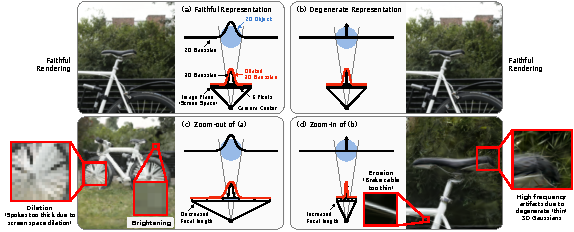
\includegraphics[width=0.88\textwidth]{figures/ch02/2311_16493_teaser.pdf}
\caption{3DGS 缩放伪影现象。尺寸正常的高斯在放大时产生锯齿（aliased），退化为极小针尖的高斯在放大时产生模糊和膨胀。图源：Yu et al.（2023.11）~\cite{2311_16493}。}
\label{fig:02_aliasing}
\end{figure}

\subsection{抗锯齿问题与挑战}

上一小节分析了伪影的根源——高斯基元尺寸固定、固定膨胀无法随采样率自适应调整。本小节介绍现有的解决方案，大致分三条路线：\textbf{频率约束}从信号处理角度限制高斯能表示的最高频率；\textbf{多尺度表示}为不同缩放级别维护独立的细节层次；\textbf{屏幕空间滤波}改进~$\alpha$-混合公式或施加屏幕空间滤波器。三条路线并不互斥，近期工作经常组合使用。

\subsubsection{频率约束路线}

下面介绍 3 条频率约束方法：Mip-Splatting（3D 频率约束 + 2D Mip 滤波器）、SA-GS（免训练的尺度自适应方案）和 AAA-Gaussians（全 3D 评估管线）。

\paragraph{3D 频率约束的开创性方案}

Mip-Splatting（2023.11）~\cite{2311_16493} 修改了原始~3DGS~的两个环节。在\textbf{训练时}为~3D~协方差添加频率约束，在\textbf{渲染时}用~2D Mip~滤波器替代固定膨胀，其余管线（优化器、ADC、光栅化器）保持不变。图~\ref{fig:02_mipsplatting}~直观展示了这两个改动。

\begin{figure}[htbp]
\centering
\resizebox{0.88\textwidth}{!}{\begin{tikzpicture}[
  box/.style={rectangle, rounded corners=4pt, draw=#1, fill=#1!10, text width=3cm, align=center, font=\small, minimum height=0.75cm},
  widebox/.style={rectangle, rounded corners=4pt, draw=#1, fill=#1!10, text width=3.5cm, align=center, font=\small, minimum height=0.75cm},
  diam/.style={diamond, draw=#1, fill=#1!8, font=\scriptsize, text width=1.8cm, align=center, aspect=2},
  biglabel/.style={font=\bfseries\small, #1},
  arr/.style={-{Stealth[length=5pt]}, thick, #1},
  >=Stealth
]
  \node[biglabel=techblue] (o_title) at (1.5, 10.6) {\textbf{原始 3DGS}};
  \node[box=techblue] (o1) at (5.7, 10.6) {3D 高斯基元};
  \node[box=techblue] (o2) at (5.7, 8.1) {投影到 2D};
  \node[box=techblue] (o3) at (5.7, 5.6) {固定膨胀\\（$\sigma_l \approx 0.3$ 像素）};
  \node[box=techblue] (o4) at (5.7, 3.1) {Tile 光栅化\\$\alpha$-混合渲染};
  \node[box=techblue] (o5) at (5.7, 0.6) {像素颜色};
  \node[biglabel=techgreen] (m_title) at (10.6, 10.6) {\textbf{Mip-Splatting}};
  \node[box=techgreen] (m1) at (15.5, 10.6) {3D 高斯基元};
  \node[box=techgreen, draw=techorange, fill=techorange!10] (m2) at (15.5, 8.1) {\textbf{3D 平滑滤波器}\\约束频率上界（训练时）};
  \node[box=techgreen] (m3) at (15.5, 5.6) {投影到 2D};
  \node[box=techgreen, draw=techorange, fill=techorange!10] (m4) at (15.5, 3.1) {\textbf{2D Mip 滤波器}\\模拟像素积分（渲染时）};
  \node[box=techgreen] (m5) at (15.5, 0.6) {像素颜色};
  \draw[arr=techblue] (o1) -- (o2);
  \draw[arr=techblue] (o2) -- (o3);
  \draw[arr=techblue] (o3) -- (o4);
  \draw[arr=techblue] (o4) -- (o5);
  \draw[arr=techgreen] (m1) -- (m2);
  \draw[arr=techgreen] (m2) -- (m3);
  \draw[arr=techgreen] (m3) -- (m4);
  \draw[arr=techgreen] (m4) -- (m5);
  \node[draw=techgray, fill=techbg, rounded corners, font=\scriptsize, text width=9cm, align=center] at (9.8, -1.9) {
    两个滤波器协同工作：3D 滤波器消除\textbf{放大}时的高频伪影，
    2D Mip 滤波器消除\textbf{缩小}时的锯齿。
    实验：Mip-NeRF360 上 $2\times$ 缩放测试 PSNR 比原始 3DGS 高 2--5 dB。
  };
\end{tikzpicture}}
\caption{Mip-Splatting vs 原始 3DGS 渲染流程对比。Mip-Splatting 在两个环节做出改动（橙色标注）：训练时添加 3D 平滑滤波器约束频率上界，渲染时用 2D Mip 滤波器替代固定膨胀。}
\label{fig:02_mipsplatting}
\end{figure}

Mip-Splatting 的核心贡献在于准确诊断了缩放伪影的双重根源。

\textbf{问题根源之一：缺乏~3D~频率约束。}如上一小节所述，固定膨胀导致了尺度歧义——优化器系统性地低估高斯的真实尺度，放大画面时出现侵蚀伪影。Mip-Splatting 的第一个改动正是针对这一问题。

\textbf{改动一：3D 平滑滤波器。}Mip-Splatting 通过~Nyquist~采样定理约束~3D~高斯的频率上界。直觉地说，它为每个高斯基元计算“训练期间最高的采样频率”，然后据此施加低通滤波，确保该高斯不包含超出采样能力的过高频率分量。

具体而言，对于第~$k$~个高斯基元，它在第~$n$~个训练视图中对应的采样频率为焦距与深度之比~$f_n/d_{n,k}$（采样频率越高，能分辨的细节越细）。取所有训练视图中的最大值，得到该高斯“应被允许的最高频率”：

\begin{equation}
\omega_k = \max_{n \in \{1,\ldots,N\}} \frac{f_n}{d_{n,k}}
\end{equation}

然后，对~3D~协方差施加高斯低通滤波。低通滤波的效果是让高斯变得更"胖"、更平滑——因为协方差矩阵控制高斯的形状和尺寸，增大协方差等价于扩大高斯的覆盖范围，从而抹去其中过细的高频细节。具体做法是在原始协方差~$\bm{\Sigma}_k$~上叠加一个滤波协方差~$\bm{\Sigma}_s = \frac{s}{\omega_k^2}\mathbf{I}$：

\begin{equation}
\bm{\Sigma}_k^{\mathrm{reg}} = \bm{\Sigma}_k + \bm{\Sigma}_s
\end{equation}

这里利用了高斯卷积仍为高斯的性质。滤波强度~$s$~为超参数，$\bm{\Sigma}_s$~对每个基元不同（依赖其可见的训练视图），每~$m$~次迭代重新计算。训练完成后，$\bm{\Sigma}_s$~成为场景表示的固有部分，不随视角变化，从而在放大时消除了高频伪影。

\textbf{问题根源之二：2D 膨胀不模拟物理成像。}如上一小节所述，缩小画面时固定膨胀导致高斯过度重叠。Mip-Splatting 进一步指出，这背后还有更深层的原因。

真实相机的每个像素不是一个数学意义上的"点"，而是一块有面积的感光区域。像素最终记录的颜色，是这块区域内所有入射光的平均值——这就是\textbf{物理像素积分}。打个比方：如果用方格纸去覆盖一幅画，每个方格的颜色不是方格中心那一个点的颜色，而是整个方格区域内所有颜色的平均。缩小画面时，每个像素对应的场景区域变大，方格也变大，应该对更大范围的颜色取平均。但原始~3DGS~的固定膨胀始终用同一个大小的高斯核去卷积，不随缩放变化——相当于用固定大小的方格去采样，无论画面放大还是缩小。

\textbf{改动二：2D Mip 滤波器。}改动一作用于\emph{训练时}的~3D~协方差，修改的是高斯基元本身的大小。但放大伪影之外还有缩小伪影——缩小画面时的问题不是高斯太小，而是原始~3DGS~的固定膨胀无法正确模拟物理像素积分。因此~Mip-Splatting~的第二个改动作用于\emph{渲染时}的~2D~投影，用~2D Mip~滤波器替代固定膨胀。该滤波器在数学上等价于将~2D~高斯与一个覆盖单个像素面积的~box~核做卷积（区别于~EWA（Elliptical Weighted Average，椭圆加权平均）滤波器覆盖~3$\times$3~像素区域）：

\[
G_k^{2D,\mathrm{mip}}(\mathbf{x}) = \frac{|\bm{\Sigma}_k^{2D}|}{|\bm{\Sigma}_k^{2D} + s\mathbf{I}|}\exp\!\Bigl(-\frac{1}{2}(\mathbf{x}-\bm{\mu}_k)^T(\bm{\Sigma}_k^{2D}+s\mathbf{I})^{-1}(\mathbf{x}-\bm{\mu}_k)\Bigr)
\]

两个滤波器协同工作。3D~滤波器在训练时约束频率上界以消除放大伪影，2D Mip~滤波器在渲染时模拟物理积分以消除缩小伪影。两者共同确保不同缩放级别下的一致渲染质量。实验表明，在~Mip-NeRF 360~数据集上单尺度训练后~2$\times$~缩放测试时，PSNR~比原始~3DGS~高~2--5~dB。

\paragraph{免训练的尺度自适应方案}

Mip-Splatting 在训练阶段修改了~3DGS~管线（添加~3D~频率约束），需要重新训练模型。SA-GS（2024.03）~\cite{2403_19615} 则选择了另一条路：\textbf{不做任何训练修改，仅在测试时作为插件应用}。它只修改渲染时的膨胀量——将固定的~$\sigma_l^2$~调整为与渲染采样率匹配的~$\sigma_l^2 r^2$（其中~$r$~为训练与渲染的采样率之比），而不改变训练时的协方差。SA-GS 首先区分了``锯齿''与``高斯尺度失配''（Gaussian scale mismatch）两个概念。3DGS 缩放伪影的根源是后者而非前者。具体地，3DGS~\cite{2308_04079}~训练时用固定~$\sigma_l = 0.3$~的高斯核膨胀投影~2D~高斯，等价于协方差从~$\bm{\Sigma}_k$~变为~$\bm{\Sigma}_k + \sigma_l^2 \mathbf{I}$（约~1.64~像素膨胀）。这使高斯投影尺度与训练分辨率/焦距耦合。SA-GS 提出~2D~尺度自适应滤波器，计算训练与渲染之间的比率~$r = R_p \cdot D_c$（$R_p$~为分辨率比，$D_c$~为焦距/距离比），据此将膨胀协方差调整为~$\bm{\Sigma}_k + \sigma_l^2 r^2 \mathbf{I}$。当~$r=1$~时退化为训练时的膨胀量，确保任意渲染设置下高斯分布与训练时一致。

在解决尺度失配后，SA-GS 进一步改进了像素颜色的计算方式。原始~3DGS~在渲染时，对每个像素只查询投影~2D~高斯在像素中心点的值——这相当于假设像素是一个无穷小的点。但真实像素有面积，像素的最终颜色应该是高斯在整个像素面积上的平均值。一个朴素的改进是超采样：在每个像素内取多个采样点再取平均，采样越多越精确，但计算量也线性增长。SA-GS 的关键洞察是：由于高斯函数有解析的累积分布函数（CDF），可以直接用公式精确计算高斯在任意区间内的积分，无需逐点采样。具体地，将~2D~高斯分解为~$x$、$y$~两个独立的~1D~高斯，每个方向上用~CDF~直接算出像素边界内的积分值：$\alpha = (\Phi_x(P_x^+) - \Phi_x(P_x^-))(\Phi_y(P_y^+) - \Phi_y(P_y^-))$。这等价于超采样数量趋于无穷的极限——精确且高效。对于像素轴与高斯轴不对齐的情况，SA-GS 将像素旋转至与高斯轴平行后计算积分，并证明了近似误差有上界。该方法无需重新训练即可达到与~Mip-Splatting~相当或更好的效果。

\paragraph{全 3D 评估管线}

前两个方法（Mip-Splatting、SA-GS）都在~2D~屏幕空间进行滤波，即先将~3D~高斯投影到~2D~再处理。AAA-Gaussians（2025.04）~\cite{2504_12811} 认为这仍然是一种近似——在~3D~空间中本可以做更精确的抗锯齿，但投影到~2D~后这个机会就丧失了。它将抗锯齿从“2D 后处理”提升为“完整的~3D~评估管线”，包含三个核心组件。

第一，\textbf{自适应~3D~平滑滤波器}。Mip-Splatting 的~3D~平滑滤波器使用训练时的最大采样频率确定固定滤波大小，渲染时不再变化。AAA-Gaussians 为每个渲染视角重新计算~3D~平滑滤波器，但发现直接照搬~Mip-Splatting~的做法会导致高斯变得过度透明。原因是这样的：当增大~3D~高斯的协方差（让它变得更"胖"），高斯的总能量不变，所以峰值会下降——就像把同一团面团摊得更薄。在传统的~2D~渲染中这不是问题，因为像素对整个~2D~高斯做积分，薄了但面积大了，总贡献不变。但~AAA-Gaussians~的~3D~评估不做积分——它沿每条光线找到高斯的最大贡献点，只取峰值。这意味着摊薄效应无法被面积增大补偿，导致高斯看起来太透明。问题对扁平的各向异性高斯尤为严重（薄饼形状的高斯沿厚度方向被进一步摊薄，峰值大幅下降）。AAA-Gaussians 的关键改进是：归一化时只考虑垂直于光线方向~$\mathbf{d}$~的两个轴的尺度变化，而忽略沿光线方向的缩放——因为沿光线方向的变化不影响光线经过时的峰值高度。具体来说，AAA-Gaussians 用以下归一化因子来补偿滤波带来的峰值下降：

\begin{equation}
\frac{|\boldsymbol{\Sigma}_{\mathbf{d}}|}{|\hat{\boldsymbol{\Sigma}}_{\mathbf{d}}|} = \frac{\mathbf{d}^\top \boldsymbol{\Sigma}^{-1} \mathbf{d}}{\mathbf{d}^\top \hat{\boldsymbol{\Sigma}}^{-1} \mathbf{d}}
\end{equation}

左边的比值~$|\boldsymbol{\Sigma}_{\mathbf{d}}|/|\hat{\boldsymbol{\Sigma}}_{\mathbf{d}}|$~就是修正后的归一化因子：分子是原始协方差在光线正交平面上的行列式，分母是滤波后协方差在同一平面上的行列式，两者的比值恰好补偿了滤波导致的峰值衰减。其中~$\boldsymbol{\Sigma}_{\mathbf{d}}$~为协方差在~$\mathbf{d}$~正交子空间上的~$2\times 2$~投影，$\hat{\boldsymbol{\Sigma}} = \boldsymbol{\Sigma} + \frac{k}{\omega'^2}\mathbf{I}$~为施加滤波后的协方差。利用逆协方差分解~$\boldsymbol{\Sigma}^{-1} = R S^{-2} R^\top$，该比值可高效计算为~$\sum_i d'^2_i / s^2_i$~与~$\sum_i d'^2_i / \hat{s}^2_i$~之比，无需显式矩阵求逆。渲染时的有效采样频率取~$\omega' = \min(\omega_{\text{train}}, \omega_{\text{render}})$，确保相机靠近时不使高斯过度缩小，远离时仍能提供有效抗锯齿。

第二，\textbf{视角空间包围}。原始~3DGS~及~HTGS~\cite{2410_08129}~在投影空间（projective space）中对高斯椭球做平面拟合来计算屏幕空间包围盒。但当高斯的椭球壳一部分位于相机后方（即~$z < 0$，在透视投影中落在观察者身后）时，投影公式会产生无效坐标，导致这些高斯被直接丢弃——画面上表现为物体突然弹出或消失（pop-in）。AAA-Gaussians 将平面拟合移至视角空间（view space），在角度域而非像素坐标域做包围计算，从根本上避免了身后坐标的投影问题。具体用平面~$\mathbf{p}_x = (\cos\alpha, 0, -\sin\alpha, 0)^\top$~和~$\mathbf{p}_y = (0, \cos\beta, -\sin\beta, 0)^\top$~求解高斯椭球在视角空间中的包围界限~$\alpha_{1,2}$、$\beta_{1,2}$，其中~$\alpha$、$\beta$~为高斯均值相对于相机在水平/垂直方向的角度。随后通过旋转步骤确保角度范围在视野范围内，再映射到屏幕坐标。

第三，\textbf{基于视锥体的~3D tile~裁剪}。原始~3DGS~使用~2D~屏幕空间~AABB（Axis-Aligned Bounding Box，轴对齐包围盒）~进行~tile~裁剪，对高度非轴对齐的椭球产生较差的包围。HTGS~\cite{2410_08129}~将裁剪提升到每~tile~的投影~2D~椭圆测试，但仍在~2D~空间操作。AAA-Gaussians 进一步为每个~tile~构造~3D~视锥体~$F$，由~4~个平面~$\mathbf{p}_{x_{1,2}} = (1, 0, 0, -x_{(m)})^\top$~和~$\mathbf{p}_{y_{1,2}} = (0, 1, 0, -y_{(m)})^\top$~定义，其中~$x_{(m)}, y_{(m)}$~为~tile~在像素坐标中的边界。裁剪时需要判断高斯在该~tile~对应的~3D~视锥体内是否有显著贡献。具体做法是找到高斯在视锥体内的最大贡献点：如果高斯的均值（中心）落在视锥体内，该均值就是贡献最大的点；如果均值在视锥体外，则将视锥体的边界平面变换到高斯的归一化坐标系中，找到平面上距高斯中心最近的点——这个点代表该高斯在视锥体内的最大可能响应。最终只保留最大响应~$\sigma_{\mathbf{x}}(\mathbf{x})^2$（即该点处高斯值的平方，衡量高斯在该~tile~内的贡献强度）高于阈值~$\sigma_T$~的~tile。为提高效率，仅投影到屏幕空间中距高斯均值最近的两个~$x/y$~平面及其对应边（而非朴素方法的全部~4~平面和~4~边）。该方法在分布外视角上显著优于先前方法。

\subsubsection{多尺度表示路线}

频率约束路线在单一尺度表示上施加滤波，但滤波本身可能引入模糊或细节损失。多尺度表示路线采取了根本不同的策略：不再试图“修复”单一尺度的问题，而是维护多个细节层次，渲染时按需选择。

\paragraph{多尺度高斯层次结构}

Yan et al.（2023.11）~\cite{2311_17089} 提出的 MS-GS 是该路线的奠基工作。MS-GS 首先需要一个指标来判断一个高斯在屏幕上“小到什么程度”——这就是“像素覆盖率”（pixel coverage）。直觉地说，把一个投影后的~2D~高斯画在屏幕上，它会呈现为一个椭圆光斑。这个光斑的边缘越往外越暗，在某个亮度阈值（$\sigma_T = 1/255$，几乎全黑）处画一条等值线，这条等值线围成一个椭圆。该椭圆沿水平轴和垂直轴的直径（以像素为单位）中较小的一个，就是像素覆盖率~$S_k$——简而言之，$S_k$~衡量的是该高斯在屏幕上实际覆盖了多少像素。当~$S_k < S_T = 2$~像素时（$S_T$~为阈值，threshold），说明这个高斯在屏幕上不到~2~个像素宽，它所包含的空间细节比单个像素还精细——按~Nyquist~定理，这种高频信号无法被当前采样率正确捕获，必然产生锯齿。

MS-GS 的多尺度构建通过高斯聚合实现。所有高斯初始化于最细层~$l=1$，经标准分裂和克隆后，在~1,000~次迭代的预热阶段后启动聚合：对每层~$l_m \geq 2$，将~$[1, l_m{-}1]$~层的高斯以~$4^{l_m-1}$~倍下采样分辨率渲染，选出像素覆盖率~$S_k < S_T$~的高斯（即在当前分辨率下太小、会产生锯齿的高斯），然后将~3D~空间划分为等大的立方体网格（每个立方体称为一个“体素”），把落入同一体素的高斯归为一组，对其属性（位置、缩放、不透明度、颜色）取平均，合并成一个更大的新高斯——这就是“体素网格分箱+平均池化”。最后按~$S_T / S_{\text{avg}}$~放大缩放因子，使合并后的高斯适应该层分辨率。新增高斯数量通常不到总数的~5\%。

渲染时采用选择性渲染策略。训练期间为每个高斯维护最大和最小像素覆盖率~$S_k^{\max}$、$S_k^{\min}$，带衰减系数更新（$S_k^{\max}$~取最大值并乘以~$\gamma_1 = 0.95$，$S_k^{\min}$~取最小值并乘以~$\gamma_2 = 1.05$）。渲染时高斯被选中的条件为：

\begin{equation}
\left(S_k \leq S_k^{\max} \cdot S_{\text{rel}}^{\max}\right) \wedge \left(S_k \geq S_k^{\min} \cdot S_{\text{rel}}^{\min} \;\vee\; S_k < S_T\right)
\end{equation}

其中~$S_{\text{rel}}^{\max} = 1.5$、$S_{\text{rel}}^{\min} = 0.5$~为相对覆盖率阈值。超出最大覆盖率高斯被过滤（过大），低于最小覆盖率且小于~$S_T$~的高斯也被过滤（过小且产生锯齿）。该方法在~4$\times$--128$\times$~缩放渲染下实现了~13\%--66\% PSNR~提升和~160\%--2400\%~渲染速度提升。

然而，MS-GS 维护多套独立高斯集合带来了额外的内存开销和管理复杂度。

\paragraph{LOD-GS：可学习采样率-滤波映射}
LOD-GS（2025.07）~\cite{2507_00554} 针对 MS-GS 多套高斯集合的内存开销问题，采取不同策略——只保留一套高斯，但为每个基元引入可学习的采样率-滤波强度映射。LOD-GS 指出 Mip-Splatting 的~3D~平滑滤波器存在固定滤波大小的局限（某些纹理被过度滤波而另一些滤波不足）。因此以采样率（$\tau = f / d$，焦距除以距离）为输入，通过~GMM（Gaussian Mixture Model，高斯混合模型）~动态预测每个基元的最优滤波强度，参数通过梯度下降端到端优化。LOD-GS 还引入了考虑相机距离变化的新合成数据集，在~SOTA~渲染质量的同时有效消除了锯齿。

\paragraph{Mipmap-GS：基元自变形替代外部滤波}
LOD-GS 的自适应滤波仍然是一种“外部施加”的约束。Mipmap-GS（2024.08）~\cite{2408_06286} 则进一步激进——完全不施加外部滤波，而是让高斯自身学会根据采样率变形。具体做法分两步。

\textbf{第一步，构造训练目标}：用当前高斯渲染一张标准分辨率的图像，然后对它做放大和缩小，分别生成“放大版伪真值”（用超分辨率模型放大）和“缩小版伪真值”（用双线性插值缩小）。这些伪真值代表“不同缩放级别下理想渲染结果应该长什么样”。

\textbf{第二步，用一致性损失引导高斯变形}：把同一个高斯模型在不同采样率下渲染，将渲染结果与对应尺度的伪真值对比，计算损失。梯度回传后，高斯的颜色、形状、大小和位置会自动调整，使得在任何缩放级别下都能渲染出与伪真值接近的结果。换言之，高斯不是被动地被外部滤波“修正”，而是主动学会在不同尺度下“变成正确的形状”。作为测试时适配方法，Mipmap-GS~在缩放场景下~PSNR~平均提升~9.25~dB（zoom-in）和~10.40~dB（zoom-out）。三种方法展示了一条从“外部管理”到“内部自适应”的演进路径：MS-GS 用多套表示应对多尺度，LOD-GS 用单套自适应滤波替代多套，Mipmap-GS 则连外部滤波也去掉，让基元自变形。

\subsubsection{屏幕空间与融合路线}

前两条路线（频率约束、多尺度表示）都在~3D~空间或基元层面解决问题。屏幕空间路线则从渲染方程本身出发，改进~$\alpha$-混合公式以更精确地处理高斯之间的空间重叠。

\paragraph{空间分布 $\alpha$-混合}

Koo et al.（2025.11）~\cite{2511_15102} 提出的 Gaussian Blending 是该路线的代表工作。传统~3DGS~将~alpha~和透射率视为标量值——在第~$i$~个高斯处的透射率~$T_i^s = \prod_{j=1}^{i-1}(1 - \int_p \alpha_j(x)\,dx)$~为单一常数，使前景高斯完全遮挡背景高斯，忽略了像素面积上的空间重叠。物理上正确的像素颜色应为空间积分~$C_p^p = \int_p \sum_{i=1}^N T_i^p(x)\,\alpha_i(x)\,c_i\,dx$，其中透射率~$T_i^p(x)$~在像素区域内随空间位置变化，但标量近似将其简化为~$C_p^s = \sum_{i=1}^N T_i^s\,c_i \int_p \alpha_i(x)\,dx$，丢失了空间遮挡信息。

Gaussian Blending 的核心创新是改变透射率的表示方式。要理解这一点，先回顾标准~3DGS~的做法：每个像素的透射率是一个标量（一个数），代表整个像素区域被前面高斯遮挡的总体程度。但像素有面积，像素内不同空间位置可能被遮挡的程度不同——比如前景高斯可能只遮住了像素的左半部分，右半部分仍然透明，能看到后面的高斯。标量透射率无法表达这种空间差异。

Gaussian Blending 的思路是：用一个矩形窗口来近似追踪"像素中哪些区域还没被挡住"。具体用三个参数描述这个窗口：中心位置~$x_i \in \mathbb{R}^2$（窗口在哪里）、尺寸~$l_i \in \mathbb{R}^2$（窗口多大）、透射率值~$t_i \in \mathbb{R}$（这个区域内有多透明）。初始时窗口覆盖整个像素（$x_1 = p$~为像素中心，$l_1 = [1,1]^\top$，$t_1 = 1$~表示完全透明）。每处理一个高斯后，窗口会收缩——被遮挡的部分被排除，窗口只保留剩余的可见区域，同时透射率值也相应更新。这样，后续高斯只在真正可见的区域内参与混合。

在数学实现上，对每个高斯泼溅，先对其~2D~协方差矩阵~$\hat{\Sigma}_i$~做特征分解得到特征值~$\lambda_1, \lambda_2$~和特征向量~$e_1, e_2$，将当前窗口旋转对齐到高斯主轴后，定义~1D~高斯的~$k$~阶矩~$I_\sigma^k(a,b) = \int_a^b x^k \exp(-x^2/2\sigma^2)\,dx$，则第~$i$~个泼溅的积分权重为：

\begin{equation}
\int w_i(x)\,dx = t_i\,o_i\,I_{\sigma_1}^0(u_1, u_2)\,I_{\sigma_2}^0(v_1, v_2)
\end{equation}

其中~$\sigma_1 = \sqrt{\lambda_1}$、$\sigma_2 = \sqrt{\lambda_2}$，$[u_1, u_2]$~和~$[v_1, v_2]$~为窗口在旋转坐标系下的边界。直观地说，这个公式计算的是：在当前窗口（未被遮挡的区域）内，第~$i$~个高斯实际贡献了多少颜色。

混合完一个高斯后，窗口需要更新——去掉已被遮挡的部分，只保留仍可见的区域。具体地，混合后的残差分布~$T_i(x)(1-\alpha_i(x))$~描述了"哪些空间位置还透着光"，对其计算零阶、一阶、二阶矩~$M_i^0, M_i^1, M_i^2$~（分别对应总面积、重心位置和散布范围），由此递推更新窗口参数：

\begin{equation}
x_{i+1} = \hat{\mu}_i' + [e_1, e_2]\,M_i^1/M_i^0, \quad l_{i+1} = \sqrt{12(M_i^2/M_i^0 - (M_i^1/M_i^0)^2)}, \quad t_{i+1} = M_i^0 / (l_{i+1,1}\,l_{i+1,2})
\end{equation}

三个更新分别对应：新的窗口中心（从重心矩计算）、新的窗口尺寸（从二阶矩计算，二阶矩越大窗口越大）、新的透射率值（剩余可见面积除以窗口面积）。每处理一个高斯，窗口就收缩一次，逐步逼近像素内真正可见的区域。整个过程在一次渲染通道中完成，不增加额外内存开销，保持实时渲染速度，作为即插即用模块可直接集成到任何~3DGS~框架中。

Gaussian Blending 解决的是~3DGS~的~$\alpha$-混合精度问题，但~3DGS~还有另一个变体——2DGS——其抗锯齿需求不同。

\paragraph{AA-2DGS：2D 高斯泼溅专用抗锯齿}
AA-2DGS（2025.06）~\cite{2506_11252} 专门针对~2D~高斯泼溅提出抗锯齿方案。2DGS 使用平面高斯盘直接在射线-泼溅交点处评估，其抗锯齿方案无法直接移植自~3DGS~的方法。AA-2DGS 引入世界空间平面平滑核（约束~2D~高斯频率基于训练视图的最大采样率）和物体空间~Mip~滤波器（利用射线-泼溅交点映射的仿射近似在每个泼溅的局部空间高效滤波），在保持~2DGS~几何精度的同时增强跨尺度渲染质量。

\paragraph{MSAA+约束优化：多样本抗锯齿引入 3DGS}
与传统图形学更接近的方案是~MSAA+约束优化（2025.08）~\cite{2508_10507}。它将传统图形学中的多样本抗锯齿（MSAA，Multi-Sample Anti-Aliasing）思想引入~3DGS。具体做法分为三步。第一，\textbf{子像素采样}：将每个像素细分为~4~个子像素（例如~$2\times 2$~网格），在每个子像素位置独立渲染，然后取平均——这样物体边缘处的像素不会被"全有或全无"地判定，而是根据高斯实际覆盖了几个子像素来按比例着色，边缘自然就平滑了。第二，\textbf{自适应权重}：不是简单取~4~个子像素的平均，而是对渲染误差大的区域赋予更大权重——误差大说明该区域的细节还没被正确捕捉，应该更重视这些子像素的渲染结果。第三，\textbf{梯度微分约束}：在物体边界处，对高斯的位置梯度施加额外的正则化，迫使高斯沿边界整齐排列，而不是随意散布——这减少了高曲率边缘和薄结构处的锯齿。

图~\ref{fig:02_antialiasing}~总结了本节介绍的四条抗锯齿技术路线及其代表性方法。

\begin{figure}[htbp]
\centering
\resizebox{0.9\textwidth}{!}{\begin{tikzpicture}[
  route/.style={rectangle, rounded corners=5pt, draw=#1, fill=#1!10,
    text width=3.2cm, minimum height=0.9cm, align=center, font=\small},
  method/.style={rectangle, rounded corners=3pt, draw=#1, fill=#1!6,
    font=\scriptsize, text width=3.0cm, align=center, minimum height=0.6cm},
  arr/.style={-{Stealth[length=4pt]}, techgray!60},
  >=Stealth
]

  \node[route=techgray, text width=4cm, font=\small\bfseries] (root) at (25.7, 5.6) {抗锯齿方法};
  \node[route=techblue] (b0) at (9.3, 3.1) {频率约束路线};
  \node[method=techblue] (b0_l0) at (3.0, 0.6) {3D平滑+2D Mip滤波\\{\tiny Mip-Splatting, AAA-Gaussians}};
  \node[method=techblue] (b0_l1) at (9.3, 0.6) {可学习滤波强度映射\\{\tiny LOD-GS}};
  \node[route=techgreen] (b1) at (22.3, 3.1) {多尺度表示路线};
  \node[method=techgreen] (b1_l0) at (15.3, 0.6) {多尺度高斯层次结构\\{\tiny MS-GS}};
  \node[method=techgreen] (b1_l1) at (22.3, 0.6) {基元自变形/尺度一致性引导\\{\tiny Mipmap-GS}};
  \node[route=techorange] (b2) at (29.1, 3.1) {屏幕空间路线};
  \node[method=techorange] (b2_l0) at (29.1, 0.6) {空间分布Alpha混合\\{\tiny Gaussian Blending}};
  \node[method=techorange] (b2_l1) at (35.0, 0.6) {2D高斯专用抗锯齿\\{\tiny AA-2DGS, MSAA+约束优化}};
  \node[route=techpurple] (b3) at (37.8, 3.1) {免训练路线};
  \node[method=techpurple] (b3_l0) at (42.2, 0.6) {测试时尺度自适应，无需重训练\\{\tiny SA-GS}};
  \draw[arr] (root) -- (b0);
  \draw[arr] (root) -- (b1);
  \draw[arr] (root) -- (b2);
  \draw[arr] (root) -- (b3);
  \draw[arr] (b0) -- (b0_l0);
  \draw[arr] (b0) -- (b0_l1);
  \draw[arr] (b1) -- (b1_l0);
  \draw[arr] (b1) -- (b1_l1);
  \draw[arr] (b2) -- (b2_l0);
  \draw[arr] (b2) -- (b2_l1);
  \draw[arr] (b3) -- (b3_l0);
  \node[draw=techgray, fill=techgray!5, rounded corners, font=\scriptsize,
    text width=12cm, align=center] at (23.6, -1.2) {核心问题：固定尺寸高斯在采样率变化时产生锯齿和膨胀/侵蚀伪影。各路线分别从频率约束、多尺度表示、屏幕空间积分和测试时适配四个角度解决此问题。};
\end{tikzpicture}}
\caption{3DGS 抗锯齿方法的四条技术路线。频率约束路线从信号处理角度限制高频分量；多尺度表示路线维护不同细节层次的高斯集合；屏幕空间路线改进混合公式；免训练路线在测试时自适应调整。}
\label{fig:02_antialiasing}
\end{figure}

\begin{takeaway}
3DGS 抗锯齿问题的根源在于高斯基元尺寸在训练后固定，无法随采样率变化自适应调整。四条技术路线各有侧重：频率约束（Mip-Splatting）从信号处理角度限制高频分量，多尺度表示维护不同细节层次的高斯集合，屏幕空间滤波改进混合公式，免训练方案在测试时自适应调整。当前趋势是多种策略的组合使用，以同时解决锯齿和膨胀/侵蚀两类伪影。
\end{takeaway}

%=====================================================================


\section{密度控制与高斯优化}
\label{sec:02_2}

密度控制是~3DGS~训练管线中最关键的机制之一。如第~\ref{sec:01_1_4}~节所述，原始~3DGS~的自适应密度控制（ADC）通过基于梯度的启发式规则（克隆、分裂、剪枝）决定高斯的增删，实现了从稀疏初始化到密集表示的自动化生长。然而，ADC~的设计存在多方面根本性局限。以下是三个层面的具体分析。

\textbf{判据层面：梯度信号不精确。}ADC~使用位置梯度的平均幅值作为致密化判据。当一个高斯覆盖包含高频细节的区域时，来自不同像素的梯度方向相反，累加后相互抵消，平均幅值低于分裂阈值。这导致该区域\emph{始终无法触发致密化}。此外，取梯度幅值的平均会丢失方向信息——无法区分“需要分裂”（梯度方向冲突）和“需要克隆”（梯度方向一致）两种截然不同的需求。

\textbf{操作层面：split/clone 互斥选择过于粗糙。}对于需要致密化的高斯，ADC~按尺度阈值二选一：大高斯执行~split，小高斯执行~clone。但实际中一个高斯可能\emph{同时需要}空间扩展（split 的作用）和局部精修（clone 的作用），这种非此即彼的互斥选择无法兼顾。此外，clone~后的高斯与父高斯重叠过高，难以独立优化。split~的子高斯随机放置，可能破坏父高斯已拟合的几何。

\textbf{宏观层面：缺乏全局约束。}ADC~没有对高斯总数、尺寸均匀性和几何一致性的全局约束。结果是高斯数量容易膨胀（训练后可达数百万），不同区域的高斯尺寸差异极大（针状与平板状并存），且产生大量不对应真实几何的浮动伪影（floaters）。这三个层面的局限共同催生了大量改进工作。

表~\ref{tab:design_research}~已总结了原始~3DGS~的设计选择与后续研究方向的对应关系。本节系统梳理~ADC~的各种改进方案。图~\ref{fig:02_adc_taxonomy}~展示了~ADC~改进方法的六条技术路线。

\begin{figure}[htbp]
\centering
\resizebox{0.85\textwidth}{!}{\begin{tikzpicture}[
  route/.style={rectangle, rounded corners=5pt, draw=#1, fill=#1!10,
    text width=3cm, minimum height=0.9cm, align=center, font=\small},
  method/.style={rectangle, rounded corners=3pt, draw=#1, fill=#1!6,
    font=\scriptsize, text width=2.8cm, align=center, minimum height=0.6cm},
  arr/.style={-{Stealth[length=4pt]}, techgray!60},
  >=Stealth
]

  \node[route=techgray, text width=4cm, font=\small\bfseries] (root) at (54.3, 5.6) {ADC 改进方法};
  \node[route=techblue] (b0) at (17.4, 3.1) {判据改进};
  \node[method=techblue] (b0_l0) at (3.5, 0.6) {梯度绝对值求和/梯度方向感知\\{\tiny AbsGS, GDAGS, DC4GS}};
  \node[method=techblue] (b0_l1) at (10.5, 0.6) {逐像素误差替代梯度\\{\tiny Revising Densification}};
  \node[method=techblue] (b0_l2) at (17.4, 0.6) {难例高斯挖掘/基元冻结修复\\{\tiny HGS, ReAct-GS}};
  \node[method=techblue] (b0_l3) at (24.1, 0.6) {方差引导/边缘感知\\{\tiny Metamon-GS, Deng et al.}};
  \node[route=techgreen] (b1) at (37.2, 3.1) {操作改进};
  \node[method=techgreen] (b1_l0) at (30.9, 0.6) {残差分裂/长轴分裂/密度保持\\{\tiny ResGS, EDC, BOGausS}};
  \node[method=techgreen] (b1_l1) at (37.2, 0.6) {局部化点管理\\{\tiny LPM}};
  \node[route=techorange] (b2) at (50.3, 3.1) {概率框架};
  \node[method=techorange] (b2_l0) at (42.7, 0.6) {SGLD采样替代启发式\\{\tiny 3DGS-MCMC}};
  \node[method=techorange] (b2_l1) at (50.3, 0.6) {Metropolis-Hastings全局探索\\{\tiny Kim et al.}};
  \node[route=techpurple] (b3) at (58.3, 3.1) {正则化};
  \node[method=techpurple] (b3_l0) at (58.3, 0.6) {原子化增殖/结构感知分布\\{\tiny AtomGS, Mini-Splatting2}};
  \node[method=techpurple] (b3_l1) at (65.0, 0.6) {频率感知/率失真优化\\{\tiny Zeng et al., BOGausS}};
  \node[route=techgray] (b4) at (70.2, 3.1) {初始化引导};
  \node[method=techgray] (b4_l0) at (70.2, 0.6) {消除致密化\\{\tiny EDGS}};
  \node[method=techgray] (b4_l1) at (74.3, 0.6) {跨场景泛化\\{\tiny GS-Net, GP-GS}};
  \node[route=techorange] (b5) at (79.9, 3.1) {可学习策略};
  \node[method=techorange] (b5_l0) at (79.9, 0.6) {神经网络预测致密化操作\\{\tiny LeGS, ConeGS}};
  \node[method=techorange] (b5_l1) at (85.9, 0.6) {哈希概率金字塔\\{\tiny Zhang et al.}};
  \draw[arr] (root) -- (b0);
  \draw[arr] (root) -- (b1);
  \draw[arr] (root) -- (b2);
  \draw[arr] (root) -- (b3);
  \draw[arr] (root) -- (b4);
  \draw[arr] (root) -- (b5);
  \draw[arr] (b0) -- (b0_l0);
  \draw[arr] (b0) -- (b0_l1);
  \draw[arr] (b0) -- (b0_l2);
  \draw[arr] (b0) -- (b0_l3);
  \draw[arr] (b1) -- (b1_l0);
  \draw[arr] (b1) -- (b1_l1);
  \draw[arr] (b2) -- (b2_l0);
  \draw[arr] (b2) -- (b2_l1);
  \draw[arr] (b3) -- (b3_l0);
  \draw[arr] (b3) -- (b3_l1);
  \draw[arr] (b4) -- (b4_l0);
  \draw[arr] (b4) -- (b4_l1);
  \draw[arr] (b5) -- (b5_l0);
  \draw[arr] (b5) -- (b5_l1);
\end{tikzpicture}}
\caption{ADC 改进方法的六条技术路线。判据改进优化触发条件，操作改进重新设计分裂/克隆机制，概率框架将致密化建模为随机采样，正则化约束高斯形状，初始化引导利用先验知识，可学习策略用神经网络替代启发式规则。}
\label{fig:02_adc_taxonomy}
\end{figure}

\subsection{ADC 的改进方法}

围绕上节分析的判据、操作和宏观三个层面的局限，后续工作形成了八条技术路线。

（1）\textbf{判据改进}：修正致密化触发条件。代表工作包括~AbsGS（梯度绝对值求和消除梯度碰撞）、GDAGS（梯度一致性比区分分裂与克隆需求）、DC4GS（方向一致性引导分裂位置）等，从梯度信号本身入手。

（2）\textbf{操作改进}：重新设计~split/clone~机制。残差分裂（ResGS）用非对称父子结构替代互斥选择；长轴分裂（EDC）用确定性对称放置替代随机偏移；局部化点管理（LPM）从渲染误差图反向定位需要操作的~3D~区域。

（3）\textbf{概率采样路线}：彻底抛弃启发式规则，将致密化建模为~MCMC~采样过程（3DGS-MCMC），或用~Metropolis-Hastings~获得全局探索能力，从概率论中获得收敛性保证。

（4）\textbf{正则化与紧凑表示}：通过约束高斯形状（尺寸均匀化、频率约束）和引入率失真优化来控制基元膨胀，从宏观层面解决高斯数量失控问题。

（5）\textbf{初始化与几何引导}：利用~SfM~点云质量、深度先验或跨场景统计等外部知识，在致密化之前就给出更好的起点，减少对~ADC~自纠正能力的依赖。

（6）\textbf{场景自适应与感知驱动}：根据场景内容（几何复杂度、纹理频率、用户关注区域）自适应调整致密化策略，例如按需局部致密化、感兴趣区域优先等。

（7）\textbf{训练加速与分解策略}：通过全局-局部分阶段致密化、SfM~引导加速等策略提升~ADC~的训练效率。

（8）\textbf{可学习密度控制}：用神经网络（强化学习、概率编码等）替代手工设计的启发式规则，让模型自己学会何时、何地、如何增删高斯。

这八条路线并不互斥——许多方法同时涉及判据改进和操作改进，或在概率框架下引入正则化。下文按路线逐一展开。

\subsubsection{致密化判据的改进}

原始~ADC~使用位置梯度的平均幅值作为致密化判据，这一设计存在三个根本缺陷。第一，\textbf{梯度碰撞（gradient collision）}：当一个大高斯覆盖包含高频细节的复杂区域时，来自不同像素的梯度方向相反、相互抵消，平均梯度幅值低于分裂阈值。这导致该区域始终无法触发致密化。第二，\textbf{信号间接性}：位置梯度仅为渲染误差的间接代理——即使某区域存在明显的渲染瑕疵，只要局部梯度平均后不够大，ADC~也不会响应。第三，\textbf{方向信息丢失}：取梯度幅值的平均抹去了方向信息，无法区分“需要分裂”（梯度方向冲突）和“需要克隆”（梯度方向一致）两种截然不同的致密化需求。以下方法分别从不同角度回应这些缺陷。

\paragraph{修正梯度信号}

AbsGS（2024.04）~\cite{2404_10484} 仅修改了原始~ADC~的致密化判据——将位置梯度的平均幅值替换为梯度绝对值求和，其他环节（分裂/克隆操作、剪枝策略、训练流程）完全不变。

\textbf{问题：梯度碰撞。}想象一个大高斯覆盖了一片有细密纹理的区域。区域左半边的像素希望高斯向左移（梯度为负），右半边的像素希望向右移（梯度为正）。在原始~3DGS~中，高斯~$G_i$~的视图空间位置梯度由逐像素子梯度累加而成：$g_{i,x} = \sum_{j=1}^m \partial L_j / \partial \mu_{i,x}$。当正负梯度幅值相近时，累加后相互抵消，平均幅值低于分裂阈值~$\tau_p = 0.0002$。这导致这个过重建的高斯\emph{始终无法触发分裂}。

\textbf{方案：梯度绝对值求和。}AbsGS~的思路很简单：不要让正负梯度互相抵消，而是把所有像素的梯度贡献都当作正值累加。具体而言，对每个分量的逐像素子梯度取绝对值后再累加：

\begin{equation}
\hat{g}_{i,x} = \sum_{j=1}^m \left|\frac{\partial L_j}{\partial \mu_{i,x}}\right|, \quad \hat{g}_{i,y} = \sum_{j=1}^m \left|\frac{\partial L_j}{\partial \mu_{i,y}}\right|, \quad \hat{g}_i = (\hat{g}_{i,x}, \hat{g}_{i,y})
\end{equation}

这一操作从根本上消除了正负梯度互相抵消的问题。$\hat{g}_i$~不参与反向传播，仅作为独立的致密化判据。它直接反映高斯覆盖区域内\emph{全部像素}的表达质量总和，而非区域整体梯度的代数残差。实验表明，以~$\hat{g}_i$~为判据仅选取~16{,}488~个高斯即可覆盖大部分过重建区域。而原始~3DGS~选取~69{,}269~个高斯却遗漏了多数过重建大高斯。AbsGS 有效恢复了高频细节并减少~10\%--20\%~的内存消耗。图~\ref{fig:02_absgs}~直观展示了梯度碰撞问题与~AbsGS~的解决方案。

\begin{figure}[htbp]
\centering
\resizebox{0.85\textwidth}{!}{\begin{tikzpicture}[
  box/.style={rectangle, rounded corners=4pt, draw=#1, fill=#1!10, text width=3cm, align=center, font=\small, minimum height=0.75cm},
  widebox/.style={rectangle, rounded corners=4pt, draw=#1, fill=#1!10, text width=3.5cm, align=center, font=\small, minimum height=0.75cm},
  diam/.style={diamond, draw=#1, fill=#1!8, font=\scriptsize, text width=1.8cm, align=center, aspect=2},
  biglabel/.style={font=\bfseries\small, #1},
  arr/.style={-{Stealth[length=5pt]}, thick, #1},
  >=Stealth
]
  \node[biglabel=techblue] at (1.7, 7.1) {原始 3DGS};
  \node[biglabel=techgreen] at (6.2, 7.1) {AbsGS};
  \node[box=techblue] (o_px) at (1.7, 5.6) {像素子梯度：$+2,\ {-3},\ +1$};
  \node[box=techblue] (o_sum) at (1.7, 3.1) {代数和：$+2 + (-3) + 1 = 0$};
  \node[box=techblue, draw=red!60, fill=red!8] (o_result) at (1.7, 0.6) {\textbf{结果}：$|0| < \tau$\\不触发致密化};
  \node[box=techgreen] (m_px) at (6.2, 5.6) {像素子梯度取绝对值：$|{+2}|,\ |{-3}|,\ |{+1}|$};
  \node[box=techgreen] (m_sum) at (6.2, 3.1) {绝对值之和：$2 + 3 + 1 = 6$};
  \node[box=techgreen] (m_result) at (6.2, 0.6) {\textbf{结果}：$|6| > \tau$\\\textbf{正确触发}致密化};
  \draw[arr=techblue] (o_px) -- (o_sum);
  \draw[arr=techblue] (o_sum) -- (o_result);
  \draw[arr=techgreen] (m_px) -- (m_sum);
  \draw[arr=techgreen] (m_sum) -- (m_result);
  \node[rectangle, rounded corners=3pt, draw=techorange, fill=techorange!8, font=\scriptsize, text width=2.4cm, align=center] at (3.9, 4.6) {
    \textbf{关键改动}\\取绝对值后累加
  };
\end{tikzpicture}}
\caption{原始 3DGS 的梯度碰撞问题与 AbsGS 的梯度绝对值求和方案。原始 3DGS 中正负梯度相互抵消导致致密化失效；AbsGS 通过取绝对值保留所有像素的贡献。}
\label{fig:02_absgs}
\end{figure}

AbsGS~解决了梯度碰撞问题，但仍有盲点：它只关注梯度的累积量，不区分“方向冲突需要分裂”和“方向一致需要克隆”这两种截然不同的需求。

\paragraph{GDAGS：梯度一致性比区分分裂与克隆}
AbsGS 通过绝对值消除了碰撞，但丢失了方向信息。GDAGS（2025.08）~\cite{2508_09239} 引入梯度一致性比（Gradient Coherence Ratio, GCR）$C_i$ 来弥补这一不足。GCR 度量高斯内梯度方向的一致程度，从而区分“方向冲突需分裂”和“方向一致需克隆”。GCR 定义为各视角下像素级子梯度的矢量和范数与标量和范数之比：

\begin{equation*}
C_i = \frac{\bigl\|\sum_{pixel}\nabla_{i,pixel^v}\bigr\|_2}{\sum_{pixel}\bigl\|\nabla_{i,pixel^v}\bigr\|_2 + \epsilon},
\end{equation*}

其中 $\nabla_{i,pixel^v} \in \mathbb{R}^2$ 为高斯 $i$ 在视角 $v$ 各像素处的位置子梯度。由 Cauchy--Schwarz 不等式可知 $C_i \in [0,1]$：$C_i \to 1$ 表示梯度方向一致、幅值有效累积；$C_i \to 0$ 表示方向冲突、幅值相互抵消。GDAGS 进一步设计非线性权重 $w_i = \beta + (1-C_i)^p$，将原始梯度范数 $\overline{\tau}_i$ 调制为 $\hat{\tau}_i = w_i \cdot \overline{\tau}_i$。这一形式的选择有两层考量。首先，为什么用幂次~$(1-C_i)^p$ 而不是线性~$(1-C_i)$？线性权重意味着~GCR~的微小变化都会等比例地影响权重，缺乏明确的决策边界——而实际需要的是：梯度方向高度一致时果断压低操作力度，方向冲突时果断放大，中间区域则平滑过渡。幂次~$p$~控制这个过渡的陡度：$p$~越大，权重在~$C_i$~的高值区下降越急促，决策越"非此即彼"；$p$~越小，过渡越平缓。其次，为什么加偏移~$\beta$？当~$C_i \to 1$（梯度完全一致）时，$(1-C_i)^p \to 0$，若不加~$\beta$~则权重为零，完全关闭分裂通道。但即使梯度方向一致，也不意味着该区域绝不需要致密化——只是不应该用分裂来处理。$\beta$~为分裂保留一个底线通道，避免信息被完全截断。

在分裂操作中直接使用 $w_i$：低~GCR（方向冲突）的大高斯获得放大的 $\hat{\tau}_i$，优先触发分裂以增强几何细节；在克隆操作中采用逆策略 $1/w_i$：高~GCR（方向一致）的小高斯被优先克隆以完成结构补充，而低~GCR~克隆则被抑制以防止局部堆积。

\paragraph{DC4GS：方向一致性引导分裂位置}
GDAGS 用一致性比区分了分裂和克隆的需求。DC4GS（2025.10）~\cite{2510_26921} 沿同一方向进一步利用方向一致性（Directional Consistency, DC）来指导分裂的\emph{具体位置}——不再随机放置子高斯，而是根据梯度方向的分布找到最优分裂点。具体而言，当一个高斯覆盖的区域内部存在结构变化（例如左半边是天空、右半边是建筑边缘），被该高斯影响的像素会给出方向冲突的梯度——左边的像素希望高斯往左移，右边的希望往右移。这种\textbf{梯度方向不均匀}的区域就是``异质区域''，说明单个高斯无法同时拟合两种不同的结构，应该分裂。反之，如果覆盖区域内各像素的梯度方向基本一致，说明高斯已经较好地拟合了该区域的几何，不需要分裂——这就是``同质区域''。为了量化这种方向均匀程度，DC4GS 将各像素的位置梯度归一化为单位向量 $u_{i,j} = g_{i,j}/\|g_{i,j}\|$，然后对它们取平均并求模长：

\begin{equation*}
\rho_i = \Bigl\|\frac{1}{N}\sum_{j=1}^{N} u_{i,j}\Bigr\|.
\end{equation*}

这个量在方向统计学中称为\textbf{圆均值}（circular mean）的模长，度量一组方向的集中程度：$\rho_i \to 1$ 表示方向高度一致（同质），$\rho_i \to 0$ 表示方向散乱冲突（异质）。基于此，DC4GS 提出~DC~加权分裂判据（DC-weighted split Criterion, DCC）：

\begin{equation*}
\hat{\tau}_i^{DC} = \frac{1}{V}\sum_{v=1}^{V}(1-\rho_{i,v})\,\|\tau_{i,v}\|,
\end{equation*}

其中 $V$ 为可见视角数，$\|\tau_{i,v}\|$ 为视角 $v$ 下沿梯度绝对值求和的幅值。$(1{-}\rho)$ 因子的作用是：同质区域（$\rho$ 高）被压低，排除不必要的分裂；异质区域（$\rho$ 低）被放大，优先触发分裂。

更进一步，DC4GS 提出~DC~引导分裂（DC-guided Split, DCS）：分裂时不再随机放置子高斯，而是沿高斯主轴（最大尺度方向）等间距采样 $N{=}5$ 个候选分裂位置，在每个位置将高斯一分为二，分别计算左、右子区域的~DC~代价 $J_l(x) = (1{-}\rho_l(x))\|\tau_l(x)\|$ 与 $J_r(x) = (1{-}\rho_r(x))\|\tau_r(x)\|$，总代价为 $J(x) = J_l(x) + J_r(x)$。最优分裂位置应使总代价最小——即分裂后左右两侧各自内部的梯度方向尽可能一致（$\rho$ 高），不再是``一边想往左、一边想往右''的混合状态。由于仅采样~5~个离散点，直接取~$\arg\min$~可能跳过真正的最优位置，DC4GS 用多项式回归将这~5~个点拟合为光滑曲线后求取极小值作为~$x_{opt}$——相比密集采样（需要~60~个点才能达到同等精度），仅用~5~个点即可稳定估计（中位~SSIM~0.987 vs 密集采样的~0.983）。该方法将高斯基元数量减少最多~30\%。

\paragraph{绕过梯度信号}

上述方法仍在修正梯度信号本身，但缺陷（2）信号间接性意味着梯度本身就不是理想的判据——即使某区域存在明显渲染误差，梯度平均后也可能不够大。Revising Densification（2024.04）~\cite{2404_06109} 从三个方面全面改进了~ADC。

\textbf{核心改进：逐像素误差替代梯度。}该方法源于一个关键观察：位置梯度对误差的\emph{变化量}敏感，但对误差的\emph{绝对值}完全盲视。想象一片草地被几个大高斯覆盖——这些高斯已经严重欠拟合，渲染结果模糊不清。但由于草地纹理高频且密集，各像素给出的梯度方向散乱，累加后相互抵消，梯度幅值接近于零。此时~ADC~误判为"不需要致密化"，实际上该区域误差极高。Revising Densification 用辅助的逐像素误差函数（如~SSIM）作为致密化判据。关键问题是如何把\emph{像素级}误差归因到\emph{高斯级}——毕竟每个像素的颜色由多个高斯混合而成。该方法的方案是按每个高斯的渲染权重~$\omega_k^\pi(u)$~将像素误差重新分配：$E_k^\pi = \sum_{u \in \text{Pix}} \mathcal{E}_\pi(u) \cdot \omega_k^\pi(u)$，然后追踪每个高斯在所有视角中的最大误差 $E_k = \max_{\pi \in \Pi} E_k^\pi$ 作为致密化评分。相比梯度阈值，误差阈值更直观——可以直接设为~"SSIM~低于多少就致密化"。

\textbf{修正克隆操作的不透明度偏差。}原始~ADC~在克隆时保持子高斯的不透明度与父高斯相同（$\alpha' = \alpha$）。但在~$\alpha$-混合渲染中，克隆前透过后方基元的权重为~$(1{-}\alpha)$，克隆后变为~$(1{-}\alpha)^2$——因为渲染光线要依次穿过两个不透明度相同的高斯。这使得克隆区域的\emph{总不透明度}被人为抬高，后方基元的贡献被压制，后续优化无法正确评估各基元的真实贡献。Revising Densification 通过调整克隆后的不透明度消除偏差：令 $(1{-}\alpha) = (1{-}\hat{\alpha})^2$，解得 $\hat{\alpha} = 1{-}\sqrt{1{-}\alpha}$，确保克隆前后后方基元看到的透射权重不变。

\textbf{基元总量控制。}原始~ADC~没有对高斯总数设上限，在复杂场景中容易导致显存溢出。该方法引入两个预算参数：高斯总数上限和每次~ADC~运行允许新增的基元数上限（设为现有基元的固定比例）。当需要致密化的高斯数超过预算时，只保留致密化评分最高的那些。达到上限后，被剪枝淘汰的高斯会被新生的替换，总数保持稳定——形成``优胜劣汰''的动态平衡，而非原始~ADC~因周期性不透明度重置导致的骤增骤降。

\paragraph{HGS：难例高斯挖掘}
HGS（2024.12）~\cite{2412_04826} 更进一步，完全绕过梯度信号，直接挖掘``难例高斯''（hard Gaussians）——即那些被~ADC~遗漏、导致渲染模糊或产生针状伪影的高斯。HGS 提出了两种互补的挖掘策略。第一种策略~PGHGS 从梯度排序中找难例。原始~ADC~对每个高斯的所有视角梯度取平均，如果大多数视角的梯度方向不一致，平均后就很小，该高斯就被忽略。但其中个别视角可能有非常大的梯度——说明那个视角下确实需要加密。PGHGS 的做法是把高斯~$G_i$~的~$n$~个视角位置梯度按幅值从大到小排列，如果第~$k$~大的梯度仍然超过阈值~$\tau_e$，就标记为难例并执行增长。这相当于说：不需要所有视角都同意，只要有足够多视角认为这个高斯需要加密就够了。第二种策略~REHGS 从渲染误差中找难例。它先找出各像素贡献最大的高斯（渲染权重最高的那个），再筛选出覆盖像素数异常多的高斯——这类高斯很可能太大了，把本该由多个高斯分别拟合的区域混在一起。然后将这些候选高斯投影回训练视角，比较渲染结果与真实图像的局部~SSIM。如果某处~SSIM~低于阈值~$\tau_q$，就确认该高斯是导致模糊的罪魁祸首。为控制总量，Effi-HGS 变体根据原始增长准则动态调节难例高斯的选取比例~$Q$。两种策略在重复纹理和少观测区域有效消除了模糊和针状伪影。

\paragraph{ReAct-GS：重要性感知致密化与基元冻结}
HGS 发现了难例高斯问题，但未触及一个更根本的现象。针对原始 ADC 在致密化判据上的根本缺陷——\textbf{梯度幅度稀释}（gradient magnitude dilution）——ReAct-GS（2025.10）~\cite{2510_19653} 发现了~HGS~未触及的``基元冻结''（primitive frozen）现象——某些高斯在训练早期快速收敛后，便陷入优化停滞，后续再也无法被更新或致密化，成为``死''基元，持续产生模糊和针状伪影。基元冻结的根本原因是\textbf{梯度信号的指数衰减}。考虑一个已经快速收敛的小尺度或针形高斯~$G_i$。在某个视角下，它投影到屏幕上的面积很小，只有中心附近的少数像素受其影响。像素~$\mathbf{p}_j$~处的高斯影响权重为~$\alpha_{i,j}^k = o_i \exp\!\bigl(-\tfrac{1}{2}(\mathbf{p}_j - \boldsymbol{\mu}_i^k)^\top \boldsymbol{\Sigma}_{2D}^{i,k}(\mathbf{p}_j - \boldsymbol{\mu}_i^k)\bigr)$——距离投影中心越远，权重以指数速度衰减至接近零。这意味着只有投影中心极少数像素的梯度能回传给该高斯，而它周围模糊区域的大量像素根本``看不到''它，无法产生梯度推动它去覆盖那些区域。冻结就此形成：高斯太小→感受野窄→只有几个像素驱动它→梯度不足以让它扩展→它永远那么小。对于针形高斯，情况类似——沿短轴方向的覆盖极窄，同样只有极少数像素贡献梯度，沿该方向的优化陷入停滞。更糟糕的是，原始~3DGS~对所有视角的梯度幅值取简单平均：$\bar{\tau}_i^L = \frac{1}{M}\sum_{k=1}^{M}\sqrt{(\frac{\partial L^k}{\partial\mu_{i,x}^k})^2 + (\frac{\partial L^k}{\partial\mu_{i,y}^k})^2}$。但一个高斯在不同视角下的渲染重要性差异很大——在某些视角下它排在深度队列前面（渲染权重~$\omega_i^k$~高，梯度有意义），在另一些视角下它被遮挡排在后面（$\omega_i^k$~接近零，梯度几乎无意义）。简单平均把有意义的梯度和无意义的梯度一视同仁，导致重要视角的信号被稀释。

这两层问题——感受野窄导致的信号微弱，加上跨视角平均导致的信号稀释——共同构成了基元冻结的完整因果链。ReAct-GS 的第一个对策是\emph{重要性感知致密化}（importance-aware densification）：不让所有视角平等发言，而是按每个视角下高斯的渲染权重~$\omega_i^k$~来加权，让高斯真正发挥作用的视角有更大话语权。

\[
\bar{\tau}_i^L = \frac{\sum_{k=1}^{M_i} \omega_i^k \sqrt{(\frac{\partial L^k}{\partial\mu_{i,x}^k})^2 + (\frac{\partial L^k}{\partial\mu_{i,y}^k})^2}}{\sum_{k=1}^{M_i} \omega_i^k}, \quad \omega_i^k = \frac{\sum_{j=1}^{m_i^k} \omega_{i,j}^k}{m_i^k},
\]

其中~$\omega_i^k$~为视角~$k$~下~$G_i$~覆盖像素的平均渲染权重，除以像素数~$m_i^k$~归一化以消除大面积高斯的偏差。在此基础上，ReAct-GS~提出\emph{密度引导克隆}和\emph{针形扰动}两种再激活机制。密度引导克隆：对达到致密化阈值的高斯~$G_i$，用~KNN（K-Nearest Neighbors，K 近邻）~计算局部密度 $d_i = \frac{1}{K}\sum_{G_j \in N_K(G_i)}\|\boldsymbol{\mu}_i - \boldsymbol{\mu}_j\|$（$K=3$），克隆体从分布~$\mathcal{N}(\boldsymbol{\mu}_i, d_i \mathbf{I}_3)$~中采样位置，而非复制到相同位置。这使稀疏区域的基元获得足够优化动量迁移至欠重建区域。针形扰动：对长短轴比超过阈值~$\tau_{ns}=0.8$~的针形基元，将较短轴放大~$1/(2s_\text{deg})$~倍（$s_\text{deg} = s_\text{min}/s_\text{max}$），以扩展感知范围恢复梯度信号，每~3000~次迭代周期性执行一次。

\paragraph{Metamon-GS 与信号统计路线}
上述方法都围绕位置梯度的\emph{均值}做文章——要么修正它，要么替代它。但均值只是信号的一阶统计量，无法区分两种截然不同的情况：一个平均梯度小的高斯，可能是因为各像素的梯度都小（确实拟合良好），也可能是因为各像素的梯度方向混乱、正负抵消（实际上需要致密化）。这两种情况在均值层面看起来一模一样。Metamon-GS（2025.04）~\cite{2504_14460} 引入颜色梯度的\emph{方差}来解决这一歧义。它的判据不只看位置梯度的平均幅值，还同时追踪每个像素处颜色梯度的变化剧烈程度。如果一个高斯覆盖的区域颜色变化剧烈（方差大），但位置梯度的平均幅值却很低，说明该区域有丰富的纹理细节未被充分建模——即使均值不触发阈值，方差信号也会将其标记为需要致密化。这种``方差引导致密化''的思路尤其擅长处理~SfM~初始化点云稀疏的区域，因为这些区域往往缺少足够的初始高斯来产生大的位置梯度，但颜色梯度的方差已经暴露了细节不足的问题。

Deng et al.（2025.08）~\cite{2508_12313} 从三个维度全面改进~ADC。在``何时致密化''方面，提出\emph{边缘感知评分}（Edge-Aware Score, EAS）——将图像边缘信息与逐像素损失结合，优先选择位于结构边缘附近的模糊高斯进行致密化。相比仅依赖梯度幅值，边缘信息能更准确地定位``应该锐利但实际模糊''的区域。在``如何致密化''方面，提出\emph{长轴分裂}（Long-Axis Split, LAS）——沿高斯最长主轴执行确定性分裂，并精心设计子高斯的位置、形状和不透明度，使分裂前后该区域的几何表示差异最小，避免原始~split~的随机偏移破坏已有拟合。在``如何缓解过拟合''方面，引入\emph{恢复感知剪枝}（Recovery-Aware Pruning）——利用不透明度恢复速度区分正常高斯和过拟合高斯，及早移除后者；同时用\emph{多步更新}（每~$N>1$~次迭代才执行一次参数更新）和\emph{增长控制}（平滑曲线约束高斯增长率）来稳定训练动态。该方法在减少高斯数量的同时提升了渲染质量。

\subsubsection{分裂与克隆操作的改进}

原始~ADC~的~split~和~clone~操作存在三方面设计缺陷。其一，\textbf{互斥选择困境}：对于需要致密化的高斯，ADC~按尺度阈值二选一——尺度大则~split，尺度小则~clone。但实际中一个高斯可能同时需要空间扩展和局部精修。其二，\textbf{clone~的高重叠}：克隆后的高斯与父高斯位置、属性相近，因梯度相似难以独立优化，往往退化为冗余。其三，\textbf{split~的形状突变}：分裂操作通过随机采样偏移生成子高斯，可能破坏父高斯原有的几何拟合状态。

\paragraph{残差分裂}

ResGS（2024.12）~\cite{2412_07494} 修改了原始~ADC~的分裂操作——用非对称的“残差分裂”替代互斥的~split/clone~选择——判据和剪枝策略保持不变。图~\ref{fig:02_resgs}~展示了残差分裂与原始操作的对比。

\begin{figure}[htbp]
\centering
\resizebox{0.85\textwidth}{!}{\begin{tikzpicture}[
  box/.style={rectangle, rounded corners=4pt, draw=#1, fill=#1!10,
    text width=3.5cm, align=center, font=\small, minimum height=0.75cm},
  diam/.style={diamond, draw=#1, fill=#1!8, font=\scriptsize,
    text width=1.8cm, align=center, aspect=2},
  biglabel/.style={font=\bfseries\small, #1},
  arr/.style={-{Stealth[length=5pt]}, thick, #1},
  >=Stealth
]

  \node[biglabel=techblue] at (3.7, 7.7) {原始 ADC};
  \node[biglabel=techgreen] at (7.5, 5.2) {ResGS 残差分裂};
  \draw[thick, techgray, dashed] (-0.1, 3.7) -- (15.2, 3.7);
  \node[box=techblue] (orig) at (3.5, 6.2) {待致密化高斯};
  \node[diam=techblue] (judge) at (3.5, 3.7) {尺度 $< S_T$?};
  \node[box=techblue] (clone) at (1.9, 1.2) {Clone\\复制到相同位置};
  \node[box=techblue] (split) at (5.5, 1.2) {Split\\二分为子高斯};
  \node[box=techgreen] (rorig) at (11.3, 6.2) {待致密化高斯};
  \node[box=techgreen] (parent) at (8.9, 3.7) {\textbf{父高斯}\\（保持原尺度）};
  \node[box=techorange] (child) at (13.2, 3.7) {\textbf{残差子高斯}\\（缩放补充细节）};
  \draw[arr=techblue] (orig) -- (judge);
  \draw[arr=techblue] (judge) -- node[above, font=\scriptsize] {是} (clone);
  \draw[arr=techblue] (judge) -- node[above, font=\scriptsize] {否} (split);
  \draw[arr=techgreen] (rorig) -- (parent);
  \draw[arr=techorange] (rorig) -- (child);
  \node[draw=techgray, fill=techbg, rounded corners, font=\scriptsize, text width=9cm, align=center]
    at (11.0, 1.9) {
    \textbf{非对称设计消除互斥选择}：父高斯保持原有尺度扩展空间覆盖，子高斯以更细粒度补充局部细节。
  };
\end{tikzpicture}}
\caption{原始 3DGS 的互斥 split/clone 操作 vs ResGS 的残差分裂。原始 ADC 按尺度阈值二选一；ResGS 的残差分裂为非对称设计——父高斯保持原尺度，子高斯缩小补充细节。}
\label{fig:02_resgs}
\end{figure}

针对互斥选择困境，ResGS 引入了\emph{残差分裂}（Residual Split）操作——为待致密化高斯~$G_i$~生成一个缩小副本~$G_j$~作为残差组件，同时降低原始高斯的不透明度。具体而言，子高斯的缩放矩阵按预设因子~$\phi_s$~缩小：$\mathbf{S}_j = \frac{1}{\phi_s}\mathbf{S}_i$；旋转、SH~系数和不透明度直接继承父高斯（$R_j = R_i$，$\text{SH}_j = \text{SH}_i$，$o_j = o_i$）；位置则从父高斯的协方差矩阵定义的分布中采样：$\boldsymbol{\mu}_j \sim \mathcal{N}(\boldsymbol{\mu}_i, \boldsymbol{\Sigma}_i)$。为抵消父子高斯重叠带来的密度激增，原始高斯的不透明度乘以衰减因子~$\phi$：$o'_i = \phi \cdot o_i$。这种非对称设计消除了原始~split/clone~的互斥选择——父高斯保持原有尺度扩展空间覆盖，子高斯以更细粒度补充局部细节。残差分裂配合一个从粗到细的训练管线：训练分~$L$~个阶段（默认~$L{=}3$），每个阶段使用图像金字塔中不同分辨率的图像作为监督——先在低分辨率图像上训练，让高斯快速建立粗略的几何覆盖，然后逐步切换到更高分辨率，让残差分裂不断补充细节。此外，ResGS 为每个高斯赋予一个``细度等级''~$l_i$（新建的高斯继承父高斯的等级），在每阶段的若干子阶段中，等级较低（即较粗）的高斯获得更低的致密化阈值，优先被残差分裂——确保粗高斯先被精修，细高斯后补完，避免在已有足够细节的区域浪费操作。

\paragraph{长轴分裂与密度保持分裂}
ResGS 用残差机制解决了互斥困境，但~split~本身的形状突变问题仍需修正。EDC（2024.11）~\cite{2411_10133} 分析了原始~clone~的高重叠和~split~的形状突变，提出\emph{长轴分裂}（Long-Axis Split）：沿高斯最长主轴执行确定性的对称分裂——子高斯沿长轴两侧对称放置，间距设为原始高斯最大半径以防重叠；子高斯沿长轴的半径缩短为原始的~$1/2$，其余轴半径缩至原始的~$85\%$；每个子高斯的不透明度降为原始的~$60\%$，以补偿分裂后从单中心变为双中心带来的密度分布变化，并缓解渲染光线依次穿过两个子高斯时的不透明度偏差问题。EDC~还配套提出了与不透明度重置周期联动的剪枝策略。其核心观察是：不透明度重置后，正常高斯和过拟合高斯展现出不同的恢复行为。正常高斯代表真实几何，多个视角的渲染误差一致地产生正梯度，驱动其不透明度迅速回升；过拟合高斯则是在少数视角的误差驱动下生成的，不同视角对它的需求互相矛盾——某些视角希望它存在，另一些则不需要——导致梯度信号正负抵消，恢复缓慢甚至振荡。利用这一差异，在每次不透明度重置后延迟若干次迭代再执行低不透明度剪枝，即可精准移除那些未能恢复的过拟合基元。该策略后被~Deng et al.~发展为更完善的恢复感知剪枝（见上文）。BOGausS（2025.04）~\cite{2504_01844} 的核心洞察是：分裂操作会扰动损失函数，导致训练不稳定。解决方案是将密度保持约束离线预计算为查找表，训练时直接查表获取最优分裂参数，实现"约束内置、在线零求解"的轻量化致密化。BOGausS（2025.04）~\cite{2504_01844} 同样沿最长主轴执行分裂，均值偏移量设为~$\delta = \gamma \cdot s$（$\gamma = 0.3$，$s$~为分裂轴方向的尺度），并通过一个预计算查找表自适应调整子高斯的尺度和不透明度。该查找表的构建过程是：在训练开始之前，对密度保持方程（即要求两个子高斯密度之和精确等于母高斯密度）进行数值求解，将不同母高斯尺度和不透明度组合下的最优子高斯参数离线存储为查找表。训练时只需查表即可获得参数，无需在线求解：

\[
(s_{\text{child}},\, o_{\text{child}}) = \text{SplitAdaptation}(s_{\text{mother}},\, o_{\text{mother}}),
\]

从而消除分裂引起的损失函数扰动。该方法完全丢弃~clone~操作，仅依赖密度保持的~split~完成致密化。

\paragraph{局部化点管理}

上述方法改进了~split/clone~操作本身，但~ADC~还有另一个盲区——它无法识别所有需要加密的~3D~区域，也缺乏处理错误高斯的机制。LPM（2024.06）~\cite{2406_04251} 从渲染误差图出发，利用多视角几何约束和特征映射定位导致误差的~3D~高斯点，在识别区域执行加密并重置前方高斯的不透明度。具体而言，LPM~的工作流程分为三个阶段。

（1）\textbf{误差图生成}：对当前视角渲染图像并与~GT~图像对比，通过误差函数生成逐像素误差图。

（2）\textbf{跨视图~3D~误差区域定位}：首先使用~LightGlue~在当前视角与邻近参考视角之间进行局部特征匹配，得到误差区域的对应区域对~$(R_e, R_e')$。然后从各相机投影中心~$o$~沿像素方向~$d$~以锥形投射射线，锥半径~$r_{\text{Cone}}$~设为~2D~误差区域最小外接圆半径。两个视角的锥体射线交点的最小包围球即为~3D~误差源区域~$R_{\text{zone}}$。

（3）\textbf{局部点操作}：在~$R_{\text{zone}}$~内执行针对性操作——若区域内有高斯则降低致密化阈值执行局部加密（小高斯沿梯度方向克隆，大高斯分裂）；若区域稀疏则在区域中心添加新高斯；若前方高斯具有最高不透明度（可能遮挡有效点导致深度估计错误），则重置其不透明度以纠正几何。此外，LPM~根据区域密度自适应剪枝低不透明度点以控制模型膨胀。作为通用插件，LPM~可无缝集成到静态~3DGS~和动态~4DGS~模型中。

\paragraph{误差驱动与等价重组}

上述方法改进了单次分裂/克隆操作的几何设计，但都保持一个共同假设：每次分裂产生固定数量的子高斯。AdpSplit（2026.05）~\cite{2605_06876} 打破这一假设，用误差区域驱动的自适应分裂替代标准的固定~$N{=}2$~随机分裂。标准~split~将每个高斯无差别地分成~2~个子高斯，子高斯位置随机偏移——不论该区域实际需要多少个子高斯、分别覆盖哪里。AdpSplit~的做法是先对待分裂高斯渲染采样视角，识别误差高且该高斯是主要贡献者的像素，然后按误差等级将这些像素分组为连通区域——每个区域生成一个子高斯，子高斯的数量由误差空间结构决定而非固定常数。子高斯的位置通过沿回投影射线最小化与父高斯的马氏距离确定，尺度和旋转从误差区域的~PCA~方向推导，颜色取区域中心的真值像素。跨视角产生的冗余子高斯通过马氏距离和颜色相似度合并，并设置每父高斯的最大子高斯数上限以防止爆炸。作为即插即用的分裂操作替换，AdpSplit~在~Mip-NeRF 360~等数据集上减少~9.2\%–22.3\%~的训练时间。

ReorgGS（2026.05）~\cite{2605_08739} 不直接修改~split/clone/prune~操作，而是针对一个训练后问题——\emph{参数化退化}：收敛后的~3DGS~模型常含有高不透明度浮游体阻挡梯度到达真实表面，以及冗余重叠簇导致参数耦合。ReorgGS~的核心思路是将收敛的高斯集合视为高斯混合概率场~$P(\mathbf{x}) = \sum_i \alpha_i \mathcal{N}(\mathbf{x} | \boldsymbol{\mu}_i, \boldsymbol{\Sigma}_i)$，从中重新采样一组新高斯：以不透明度为概率做分类采样选择源高斯（排除体积以避免放大异常大高斯），从源高斯分布中采样新中心，再用~kNN~估计局部协方差获得各向异性的形状参数，所有新高斯以低不透明度（$0.01$）初始化后继续训练。与标准的不透明度重置不同，ReorgGS~重建了中心位置、形状和重叠结构，而不仅仅是重置不透明度。作为后训练插件，ReorgGS~可迭代应用，在~vanilla~3DGS、3DGS-MCMC~等基线上提升训练~PSNR~约~0.5~dB、测试~PSNR~约~0.14~dB，同时减少冗余重叠带来最高~12.8\%~的渲染加速。

\subsubsection{概率采样与~MCMC~路线}

上述改进方案虽然从判据和操作层面修补了~ADC，但本质上仍是在启发式规则框架内打补丁——阈值敏感、缺乏理论收敛保证、需要人工调参等固有局限无法根除。一条更激进的路线是彻底抛弃启发式规则，将高斯致密化建模为严格的概率采样过程，从~MCMC（Markov Chain Monte Carlo，马尔可夫链蒙特卡洛）~理论中获得收敛性保证。

3DGS-MCMC（2024.04）~\cite{2404_09591} 从根本上替代了原始~ADC~的整个启发式框架。它用~SGLD（Stochastic Gradient Langevin Dynamics，随机梯度朗之万动力学）~随机更新替代确定性梯度下降，用”重定位”替代~clone/split/prune~三个操作，用~L1~正则化替代固定阈值剪枝。唯一保持不变的是渲染管线和损失函数。图~\ref{fig:02_mcmc}~对比了原始~ADC~与~3DGS-MCMC~的完整流程。

\begin{figure}[htbp]
\centering
\resizebox{0.78\textwidth}{!}{\begin{tikzpicture}[
  box/.style={rectangle, rounded corners=4pt, draw=#1, fill=#1!10, text width=3cm, align=center, font=\small, minimum height=0.75cm},
  widebox/.style={rectangle, rounded corners=4pt, draw=#1, fill=#1!10, text width=3.5cm, align=center, font=\small, minimum height=0.75cm},
  diam/.style={diamond, draw=#1, fill=#1!8, font=\scriptsize, text width=1.8cm, align=center, aspect=2},
  biglabel/.style={font=\bfseries\small, #1},
  arr/.style={-{Stealth[length=5pt]}, thick, #1},
  >=Stealth
]
  \node[biglabel=techblue] at (-0.6, 17.1) {原始 ADC};
  \node[biglabel=techgreen] at (-0.6, 9.6) {3DGS-MCMC};
  \draw[thick, techgray, dashed] (-0.6, 11.9) -- (9.2, 11.9);
  \node[box=techblue] (grad) at (2.0, 15.6) {位置梯度 $> \tau$?};
  \node[box=techblue] (opac) at (7.2, 15.6) {不透明度 $< \epsilon$?};
  \node[box=techblue] (clone) at (1.4, 13.1) {Clone\\复制高斯};
  \node[box=techblue] (split) at (4.3, 13.1) {Split\\二分高斯};
  \node[box=techblue] (prune) at (7.2, 13.1) {Prune\\删除低不透明度};
  \node[box=techblue] (adc_out) at (4.3, 10.6) {更新后高斯集合};
  \node[box=techgreen, draw=techorange, fill=techorange!10] (sgld) at (4.3, 8.1) {\textbf{SGLD 更新}\\$+ \eta_{\mathrm{noise}} \epsilon_\theta$};
  \node[box=techgreen] (active) at (5.8, 5.6) {活跃高斯\\$\alpha_i > 0.005$};
  \node[box=techgreen, draw=techorange, fill=techorange!10] (dead) at (2.8, 5.6) {\textbf{死亡高斯}\\$\alpha_i < 0.005$};
  \node[box=techgreen, draw=techorange, fill=techorange!10] (reloc) at (2.8, 3.1) {\textbf{重定位}\\死亡$\to$活跃位置};
  \node[box=techgreen] (reg) at (6.3, 3.1) {L1 正则化};
  \node[box=techgreen] (mcmc_out) at (4.5, 0.6) {更新后高斯集合};
  \draw[arr=techblue] (grad) -- (clone);
  \draw[arr=techblue] (grad) -- (split);
  \draw[arr=techblue] (opac) -- (prune);
  \draw[arr=techblue] (clone) -- (adc_out);
  \draw[arr=techblue] (split) -- (adc_out);
  \draw[arr=techblue] (prune) -- (adc_out);
  \draw[arr=techorange] (sgld) -- (active);
  \draw[arr=techorange] (sgld) -- (dead);
  \draw[arr=techorange] (active) -- (reloc);
  \draw[arr=techgreen] (active) -- (reg);
  \draw[arr=techorange] (dead) -- (reloc);
  \draw[arr=techorange] (reloc) -- (mcmc_out);
  \draw[arr=techgreen] (reg) -- (mcmc_out);
  \node[draw=techgray, fill=techbg, rounded corners, font=\scriptsize, text width=9cm, align=center] at (4.4, -1.9) {
    Clone/Split/Prune 三个启发式操作被统一为\textbf{SGLD 更新 + 重定位}，从 MCMC 理论获得收敛保证。
  };
\end{tikzpicture}}
\caption{原始 ADC 的启发式框架 vs 3DGS-MCMC 的概率采样框架。原始 ADC 使用梯度阈值驱动的 clone/split/prune 三种操作；3DGS-MCMC 用 SGLD 更新 + 重定位 + L1 正则化统一替代，从 MCMC 理论获得收敛保证。}
\label{fig:02_mcmc}
\end{figure}

\textbf{核心洞察：梯度下降就是概率采样。}要理解这一等价性，需要转换视角。标准~3DGS~的训练目标是最小化渲染损失~$\mathcal{L}(\theta)$，梯度下降的每一步都在让参数朝损失更低的方向移动。现在换一个等价的视角：如果把损失~$\mathcal{L}(\theta)$~看作某个概率分布的负对数，即~$\mathcal{L}(\theta) = -\log p(\theta)$，那么最小化~$\mathcal{L}$~就等价于最大化~$p(\theta)$~——也就是寻找概率最大的参数配置。SGLD（随机梯度朗之万动力学）是一种概率采样方法，其更新规则为~$\theta \leftarrow \theta + a \nabla_\theta \log p(\theta) + b \epsilon$。前两项~$\theta + a \nabla_\theta \log p(\theta)$~恰好就是梯度下降（因为~$\nabla_\theta \log p = -\nabla_\theta \mathcal{L}$），第三项~$b \epsilon$~是随机噪声。所以，当~$b=0$（不加噪声）时，SGLD~退化为梯度下降——标准~3DGS~的每一步优化，本质上就是在对应概率分布上做一步无噪声采样。3DGS-MCMC~的关键操作就是加上这个噪声项：让参数在朝高概率区域移动的同时，保留一定的随机探索，避免被困在局部最优。具体地，3DGS-MCMC~在梯度更新中添加精心设计的噪声项：

\[
\theta \leftarrow \theta - \eta_{\text{lr}} \nabla_\theta \mathcal{L} + \eta_{\text{noise}} \cdot \epsilon_\theta,
\]

噪声项~$\epsilon_\theta$~的构造是关键——它必须与高斯自身几何形状匹配：

\[
\epsilon_\theta = \eta_{\text{noise}} \cdot \sigma(-k(t - \alpha)) \cdot \Sigma^{\frac{1}{2}} \cdot \mathcal{N}(0, I),
\]

这里~$\Sigma^{\frac{1}{2}}$~确保噪声的各向异性轮廓与高斯自身协方差一致——细长高斯沿长轴方向获得更大探索范围，沿短轴方向则保持紧凑。$\sigma(\cdot)$~为~sigmoid~函数，在默认剪枝阈值处形成急剧过渡。不透明度~$>0.005$~的”活跃”高斯噪声被大幅抑制（避免破坏已收敛的梯度引导），不透明度~$<0.005$~的”死亡”高斯获得强噪声（探索空间中未被覆盖的区域）。噪声仅作用于高斯位置，实验发现对不透明度、尺度和颜色添加噪声反而有害。

\textbf{重定位替代 clone/split/prune。}原始~ADC~需要三种操作：clone~增加基元、split~分裂基元、prune~删除基元，每种操作都有各自的阈值和触发条件。3DGS-MCMC~用一个统一的\emph{重定位}（relocation）操作替代了全部三者。重定位的出发点是一个简单问题：与其创建新高斯或删除旧高斯，为什么不把”没用”的高斯直接搬到”需要”它的地方？为此，3DGS-MCMC~引入~L1~正则化项~$\lambda_{\alpha} \sum_i |\alpha_i|$~和~$\lambda_{s} \sum_{i,j} |\text{eig}_j(\Sigma_i)|$~分别惩罚不透明度和尺度。这些正则项在训练过程中持续压制冗余高斯的参数——当某个高斯的贡献被周围高斯覆盖时，光度损失的梯度对它的驱动力很弱，而正则化持续将其不透明度推向零。最终，冗余高斯的不透明度降至~$0.005$~以下，几乎不影响渲染——这就是``死亡高斯''。重定位操作每~100~次迭代执行一次：随机选取一个不透明度较高的活跃高斯作为目标（按不透明度值做多项式采样，越重要的高斯越容易被选中），然后将~$N-1$~个死亡高斯移到该目标的位置附近。关键约束是：移动前后该区域的渲染结果必须尽可能不变。

为此，原活跃高斯和~$N-1$~个重定位高斯被赋予相同的不透明度~$\alpha^{\text{new}} = 1 - (1-\alpha^{\text{old}})^{1/N}$。这个公式的含义是：$N$~个不透明度为~$\alpha^{\text{new}}$~的高斯经~$\alpha$~混合后的合成不透明度为~$1-(1-\alpha^{\text{new}})^N$，令其等于原活跃高斯的~$\alpha^{\text{old}}$~即可解出~$\alpha^{\text{new}}$。协方差也相应缩放。这与原始~clone~操作有本质区别：克隆会直接复制高斯导致密度翻倍，破坏渲染一致性；重定位则通过精确的不透明度分解保持渲染不变性，在~MCMC~框架中是合法的状态跳转。需要注意，3DGS-MCMC~中高斯的总数是固定的——训练开始时有多少个高斯，训练结束时还是多少个。没有创建，也没有销毁。所有密度调整都通过”杀掉”冗余高斯（L1 正则化将其不透明度压至~0.005 以下）再``复活''到新位置（重定位）来完成。该方法无需精心调整的~clone/split~阈值，对初始化具有鲁棒性。

\paragraph{MH 接受-拒绝采样与全局探索}
3DGS-MCMC 使用~SGLD~作为采样策略，但~SGLD~的每步更新始终沿梯度方向加噪声，属于局部探索——无法跳转到远离当前高斯群的未覆盖区域。Kim et al.（2025.06）~\cite{2506_12945} 将致密化重构为~MH（Metropolis-Hastings）概率采样过程，获得了全局探索能力。该方法的思路可以概括为两步：\emph{提出}一个新增高斯的方案，然后\emph{检验}它是否真的改善渲染质量——只保留确实有用的。

\textbf{第一步：在哪里添加高斯？}每次致密化时，选取若干训练视角，计算每个像素的渲染误差（结合~SSIM~误差、$\mathcal{L}_1$~误差和渲染不透明度），融合为一个``重要性分数''~$s(p) \in (0,1)$，标记哪些像素处的渲染结果最差。然后将~2D~像素的重要性投影到~3D~空间，得到每个已有高斯的``被选中概率''~$P_{\text{pick}}(i)$——周围渲染误差越大的高斯，越可能被选中。被选中的高斯~$G_i$~将作为新加高斯的``锚点''。

添加分两轮：第一轮用较大的随机偏移（$\epsilon \sim \mathcal{N}(0, \sigma_{\text{coarse}}^2 I)$），在锚点附近大范围撒点，快速覆盖大片空白区域；第二轮用较小的偏移（$\sigma_{\text{fine}}^2 < \sigma_{\text{coarse}}^2$），在第一轮之后仍有高误差的局部精修。每个新加高斯的位置为~$\boldsymbol{\mu}_i + \epsilon$，其余参数（协方差、颜色等）继承锚点高斯。两轮设计的原因很简单：只用大偏移，定位不精确；只用小偏移，走不远——分两步先粗后精。

\textbf{第二步：要不要接受这个高斯？}并非每个提议都值得接受——如果新加的高斯落在已有足够覆盖的区域，它不仅无益，反而浪费资源。MH~接受测试就是做这个裁决：比较``加入新高斯后''和``加入前''两种状态的好坏。这里``好坏''由两个因素决定：渲染质量是否提升（光度损失是否下降），以及新高斯是否落入了已经很拥挤的区域。后者通过一个体素级先验实现：将~3D~空间划分为体素网格，统计每个体素内的高斯数量~$c_\Theta(v)$，用~$\sum_v \log(1 + c_\Theta(v))$~作为惩罚项。这个惩罚的设计是：空体素几乎不受罚，但体素越拥挤惩罚越重——多个高斯叠加在一起虽然能把渲染误差压到零，但纯属浪费。综合渲染质量和体素拥挤度，定义``总能量''~$E(\Theta) = \mathcal{L}(\Theta) + \sum_v \log(1 + c_\Theta(v))$。MH~接受概率的形式为：

\[
\alpha(\Theta' | \Theta_t) = \min\!\left(1,\; \frac{e^{-E(\Theta')}\,q(\Theta_t | \Theta')}{e^{-E(\Theta_t)}\,q(\Theta' | \Theta_t)}\right),
\]

直觉含义：如果新状态~$\Theta'$~的总能量更低（渲染更好且不拥挤），则~$e^{-E(\Theta')} > e^{-E(\Theta_t)}$，接受概率接近~$1$，几乎一定接受；反之，如果新状态更差，则以较低概率随机接受（避免完全丧失探索能力）。通过随机数~$u \sim \mathcal{U}(0,1)$~裁决：$u < \alpha$~则接受，否则拒绝。与~3DGS-MCMC~的~SGLD~每步无条件接受噪声更新不同，MH~通过这一检验过滤低质量候选，使高斯数量的增长更有针对性。

该方法同样采用重定位机制复用低不透明度高斯（$\alpha_i < 0.005$）。与~3DGS-MCMC~固定高斯总数不同，Kim et al.~允许总数动态变化——候选生成增加高斯，体素先验和~L1~正则化压制冗余高斯，两者共同驱动数量趋于合理水平。该方法在所有基准场景上达到~30 dB PSNR~平均比~3DGS-MCMC~快约~2.2~分钟，同时使用更少的高斯数量。

\subsubsection{正则化与紧凑表示}

ADC~的”自由生长”策略有一个根本缺陷：没有任何全局约束来管束高斯的几何属性。后果是两方面——高斯尺寸极度不均匀（小至针状、大至覆盖整个平面），以及数量膨胀带来的内存和渲染开销。正则化方法正是为了弥补这一缺陷：通过显式约束高斯的形状和分布，在保持渲染质量的同时压缩模型体积。

\paragraph{尺寸均匀化}

针对 3DGS 原版自适应密度控制（ADC）在优化优先级上的根本缺陷——方法倾向于优先放大覆盖大面积的大高斯，而非增殖用于填补几何间隙的小高斯，导致细节区域的高斯因"欠致密化"而产生噪声几何与模糊伪影——AtomGS（2024.05）~\cite{2405_12369} 提出了\textbf{原子化增殖}（Atomized Proliferation）策略，核心思想是：与其让高斯自由变形来近似填补间隙，不如用尺寸均匀的原子高斯通过精确增殖来忠实贴合几何表面。AtomGS（2024.05）~\cite{2405_12369} 的思路是”原子化增殖”：先从~SfM~点对距离中确定一个”原子尺度”~$S$，将尺度低于~$S$~的高斯强制设为各向同性球体（原子高斯），尺度参数固定、不参与反向传播；高于~$S$~的大高斯保留传统椭球形态，覆盖背景。训练过程中，原子高斯的尺度按几何级数从粗到细递减（先大球快速覆盖间隙，再小球精修细节），致密化时反转克隆逻辑——允许大高斯克隆增殖、逐步降低分裂阈值让更多高斯分裂为原子高斯，剪枝时则提高不透明度重置频率淘汰冗余大高斯。再搭配边缘感知法线损失（平坦区域加强平滑、边缘区域保留细节），AtomGS~在平滑平坦表面的同时保留精细细节。

\textbf{设计动机。}在原始~3DGS~中，高斯的尺度参数完全由反向传播自由优化，这带来两个问题。其一，细节区域的高斯倾向于拉伸成各向异性椭球来”近似覆盖”几何间隙，而非真正贴合表面——相当于用一块不规则的补丁勉强盖住一个洞。其二，不同区域的高斯尺寸差异极大，难以保证统一的几何精度。AtomGS~的核心思想是反其道而行：与其让高斯自由变形来填补间隙，不如用尺寸固定的各向同性球体（原子高斯）通过增殖来精确填充；同时，覆盖大面积平坦区域的高斯仍然保持传统椭球形态。

\textbf{原子高斯的尺度约束。}AtomGS~首先需要确定一个”原子尺度”~$S$。做法是从~SfM~输入点集出发，将所有点对距离排序后取第~$i$~百分位数作为~$S$——直观上就是让原子高斯的大小与相邻点之间的典型间距匹配。这个尺度把高斯分为两类：尺度低于~$S$~的归为”原子高斯”（Atom Gaussian），强制设为各向同性球体~$s_1 = s_2 = \cdots = s_n = (S)^{1/3}$；尺度高于~$S$~的保持传统各向异性椭球，用于覆盖大面积背景区域。原子高斯一旦被标记，其尺度参数即固定，从此不再参与反向传播优化。

\textbf{原子尺度的几何级数递减。}原子高斯的尺度虽不通过梯度下降调整，但通过几何级数逐迭代递减：$S_n = S_{n-1} \cdot r^{n-1}$，其中公比~$r = \sqrt[t_a]{p}$，$t_a$~为原子化迭代总次数，$p$~为最终尺度相对于初始~$S$~的比例。这一设计的理由是：训练初期需要较大的原子高斯快速覆盖几何间隙，后期则需更小的原子高斯逐步精化细节。几何级数递减确保尺度从粗到细平滑过渡，而非突变。

\textbf{增殖与剪枝策略。}在致密化侧，AtomGS~允许大尺度高斯通过克隆操作增殖（原始~3DGS~仅对小高斯克隆），并逐步降低分裂梯度阈值，让更多高斯满足分裂条件，产生的子高斯直接标记为原子高斯，优先填补几何间隙。在剪枝侧，AtomGS~提高不透明度重置频率，促使表示大面积平坦表面的冗余高斯合并消失，同时保留捕获精细高频细节的高斯。接下来介绍的 Mini-Splatting2 则从空间分布均衡性的角度解决类似问题。

\paragraph{空间分布均衡化}

AtomGS 直接约束高斯形状，但未考虑空间分布的均衡性。Mini-Splatting2（2024.11）~\cite{2411_12788} 将~3DGS~从纯粹的光度监督驱动建模转向几何调节的建模范式。该方法通过结构化重组重新安排高斯的空间分布，引入表示稀疏性约束确保均衡覆盖，并通过大幅提高致密化速率和跳过不可见高斯的更新来加速收敛，实现了~4$\times$~更少高斯和~3$\times$~更快优化。

\textbf{设计动机。}Mini-Splatting2~从几何视角重新审视~3DGS~的建模过程，识别出两个核心低效问题。第一，\emph{空间分布的不规则性}：原始~ADC~策略基于图像空间位置梯度进行阈值化致密化，但梯度大的纹理区域会过度聚集大量高斯（“重叠”冗余），而梯度相对较低的纹理区域则因未达阈值而覆盖不足（“欠重建”模糊），两者共同导致场景表示的冗余与不足并存。第二，\emph{训练动态的无区分性}：原始~3DGS~对所有高斯施加均匀更新，不考虑其几何贡献或可见性，浪费计算在被遮挡或信息量低的高斯上，延迟了场景结构的涌现。

\textbf{结构感知分布方案。}该方案包含两个协同模块，用于规整高斯的空间排列。首先是\emph{自适应高斯组织}，通过两个组件改善覆盖均衡性：（1）模糊分裂（blur split）——识别``欠重建''区域中贡献面积过大的高斯，具体地，对每个高斯计算其最大贡献面积~$S_i = \sum_{\mathbf{x}} \delta(i(\mathbf{x}) = i_{\max}(\mathbf{x}))$（即~$\alpha$-混合~中权重最大的像素总数），当~$S_i > \mathcal{T}_{\text{blur}}$（阈值~$\mathcal{T}_{\text{blur}} = \theta_{\text{blur}} \cdot H \cdot W$，$\theta_{\text{blur}} = 2 \times 10^{-4}$）时触发分裂，增加局部密度；（2）深度重新初始化（depth reinitialization）——利用多视角深度估计生成密集点云作为高斯的新初始化位置，替换原始~SfM~稀疏点云，确保更均衡的场景覆盖。在深度估计上，Mini-Splatting2~不采用~$\alpha$-混合~深度（因多高斯混合导致深度坍塌和物体错位），而是取每个像素最大贡献高斯与视线方向射线-椭球交点的中点深度~$d^{mid}_{i_{\max}}$。

其次是\emph{冗余高斯简化}，通过两个组件降低内存开销。（1）\emph{结构关键高斯保留}：渲染时，每个像素在~$\alpha$-混合~中有一个权重最大的高斯（对该像素渲染贡献最高）。如果一个高斯在至少一个像素上排第一，它就是"结构关键"的，必须保留；从未在任何像素上排第一的高斯被淘汰。（2）\emph{重要性加权随机采样}：对于需要进一步精简的高斯，不做确定性剪枝（直接删掉不重要的），而是以高斯重要性~$I_i = \sum_{j=1}^{K} w_{ij}$（跨所有相交射线的混合权重之和）为采样概率~$\mathcal{P}_i = I_i / \sum_{i} I_i$~进行加权随机采样——重要性越高，被保留的概率越大。随机采样比确定性剪枝的好处是：在低保留率下不会出现局部区域的高斯被全部删光的"空洞"问题，能更好地保留几何连续性。

\textbf{区域优先优化方案。}上述结构感知分布方案解决了"高斯放在哪里"的问题，但训练速度仍有瓶颈——原始~3DGS~每次致密化只操作约~5\%~的高斯，收敛很慢。Mini-Splatting2~从两个方面加速。一是\emph{大幅提高致密化速率}：选取在~$\alpha$-混合~中贡献权重~$w_{i_{\max}}$~排在~0.99~分位数以上的高斯（即对渲染最重要的那些），每轮克隆约~30\%~的高斯（对比原始~3DGS~的~5\%），同时通过与~3DGS-MCMC~重定位类似的不透明度分解保持渲染不变性：$\alpha^{\text{new}} = 1 - \sqrt{1 - \alpha^{\text{old}}}$，协方差相应缩放。这将致密化阶段从~15K~迭代缩短至~3K~迭代。

二是\emph{跳过不可见高斯的更新}：在光栅化预处理阶段，对第~$k$~个训练视角，高斯~$\mathcal{G}_i$~的可见性定义为~$V_i^k = \mathbb{I}(\sum_{j=1}^{J} w_{ij}^k > \tau)$（$\tau$~由~0.99~分位数确定），非可见高斯在该视角的前向和反向传播中均被跳过。该机制在~500~至~13K~迭代之间激活，将计算资源聚焦于真正可见的区域。

\paragraph{频率与率失真约束}

上述方法从几何角度约束高斯分布，另一类方法从信号处理和信息论角度入手。Zeng et al.（2025.03）~\cite{2503_07000} 从信号处理角度建立密度与尺度的一致性约束，通过缩放参数重参数化显式关联高斯数量与大小，并设计频率感知的密度控制策略——在高频区域降低阈值鼓励生成更多高斯，同时用基于尺度的过滤器移除尺度不当的高斯。BOGausS（2025.04）~\cite{2504_01844} 则借用视频压缩中的率失真优化思路——将高斯数量视为"码率"（越多模型越大），渲染误差视为"失真"，在两者之间找最优平衡。在致密化侧，该方法为每个高斯定义重建平方误差~$SE_{c,i} = \sum_p I_c\, w_i^{(c)}\,(R^{(c)}(p) - I^{(c)}(p))^2$，其中~$w_i^{(c)}$~为高斯~$i$~在相机~$c$~中的渲染权重，优先级指标基于相对贡献误差：

\[
P_{\text{SNR}}(i) = \sum_c \frac{SE_{c,i}}{\sum_j SE_{c,j}},
\]

分裂对~PSNR~增益最大的高斯（即相对误差占比最高的），而非绝对误差最大的。在剪枝侧，核心问题是判断"哪些高斯对渲染几乎没贡献"。BOGausS~为此定义有效不透明度指标~$P_{\text{prune}}(i) = \sum_c P_i^{(c)}$，其中~$P_i^{(c)} = \sum_p w_i^{(c)}(p)\, S_i^{(c)}$~为高斯~$i$~在相机~$c$~中的有效贡献——$w_i^{(c)}(p)$~是该高斯在像素~$p$~上的渲染权重，$S_i^{(c)}$~是该高斯投影到相机~$c$~的~2D~尺度，两者之积衡量该高斯在屏幕上实际覆盖了多少面积且有多不透明。该值低于阈值~$\tau_{\text{prune}} = 0.02$~的高斯被剪除，每次迭代最多剪掉~1\%~的总高斯数。该优先级体系替代了原始~3DGS~的不透明度周期性重置，在模型大小和渲染质量之间找到更好的平衡，生成比原始~3DGS~轻~10~倍的模型。

\paragraph{数量预算控制}

上述正则化方法间接限制高斯数量（通过约束形状、分布或频率），但都无法提供硬性数量上限。YOGO（2026.04）~\cite{2604_21400} 用确定性预算控制器（Deterministic Budget Controller, DBC）直接解决这一问题：用户指定目标高斯总数，DBC~通过反馈循环保证最终数量严格收敛到预设值。具体地，场景被划分为空间多边形区域，每个区域分配目标数量~$N^{\text{target}}$。每次致密化事件中执行"先剪枝后致密化"序列：先移除有效不透明度（不透明度~$\times$~透射率）低于阈值的高斯，然后计算剩余预算缺口，按动态配额~$N_{\text{densify}}(k) = \max(0, \Delta_N(k) / (K{-}k{+}1))$~选择梯度最大的高斯进行致密化——前期配额宽松、后期收紧，最终数量精确收敛。此外，YOGO~配套多项改进：面积归一化梯度累积（消除大高斯偏差）、沿主轴的三元组致密化（替代标准~split/clone~）、以及多传感器数据污染过滤协议。在超密集采样的~Immersion v1.0~数据集上，YOGO~仅用~150~万高斯即在渲染质量上超越使用~428~万高斯的~AbsGS。

\subsubsection{初始化与几何引导}

ADC 的核心假设是“从稀疏点云出发，通过致密化逐步补全”。但如果初始化本身就已经足够好，ADC 的负担将大幅减轻。以下方法从不同角度改善初始化。

\paragraph{消除与改善致密化}

最激进的策略是 EDGS（2025.04）~\cite{2504_13204}——完全消除致密化过程。其核心动机是：标准~3DGS~的坐标位移量（初始位置到收敛位置的~$L_2$~距离）极大，说明高斯在优化过程中发生了大幅位移才到达正确位置。如果能一开始就把高斯放在接近正确的位置，优化器只需微调即可。EDGS~的实现分三步。第一步，\textbf{密集对应估计}：对参考图~$I^i$，用预训练匹配网络 RoMa~\cite{2305_15404} 估计它与邻域图~$I^j$~之间的逐像素正向扭曲场~$W^{i \to j} \in \mathbb{R}^{2 \times H \times W}$~和对应置信度~$c^{ij} \in \mathbb{R}^{H \times W}$。第二步，\textbf{三角化}：将匹配的~2D~像素对~$(u_k^i, v_k^i)$、$(u_k^j, v_k^j)$~通过投影矩阵~$P^i, P^j$~提升到~3D。具体地，对每个匹配点~$k$，从~$4 \times 3$~投影矩阵的各列构造线性方程组~$A\,\mathbf{g}_k^x = \mathbf{b}$，用最小二乘求解高斯的~3D~齐次坐标：

\begin{equation*}
\mathbf{g}_k^x := \arg\min_{\mathbf{x}} \|A\,\mathbf{x} + \mathbf{b}\|^2, \quad \mathbf{g}_k^x = [x_k, y_k, z_k, 1]^T.
\end{equation*}

第三步，\textbf{采样分布}：三角化产生的~3D~点数量庞大（每对图可能产生数十万个匹配），直接全部用作初始高斯既不现实也不必要——其中包含大量误匹配。EDGS~的策略是按概率采样一个子集，只保留可靠的点。可靠性由两个指标衡量：\textbf{匹配置信度}~$c^{ij}$（匹配网络对该对应的把握）和\textbf{重投影误差}~$\delta_k$（三角化后重投影回原图的偏差，越小说明几何越自洽）。EDGS~据此构造采样分布：

\begin{equation*}
p^i(k) \propto \prod_{j \in \mathcal{N}_i} \bigl(p_{\text{corr}}^{ij}(k) \cdot p_{\text{proj}}^{ij}(k)\bigr),
\end{equation*}

其中~$p_{\text{corr}}^{ij}$~仅在置信度超过阈值~$\theta_{\text{corr}}$~的点上均匀分布，$p_{\text{proj}}^{ij}$~仅在重投影误差低于阈值~$\theta_{\text{proj}}$~的点上均匀分布——不满足条件的点概率为零，直接排除。最后，EDGS~从参考图的像素颜色出发，收集每个高斯在~$n$~个视角方向的~RGB~观测~$O_k \in \mathbb{R}^{n \times 3}$，通过求解球谐系数~$H_k = Y_k^{+}O_k$（$Y_k \in \mathbb{R}^{n \times 16}$~为球谐基矩阵）完成颜色初始化。整个流程完全绕过~SfM~和~ADC，高斯在优化中的坐标位移量减少~50~倍、轨迹长度减少~30~倍，仅~5K~步即可达到效率优化方法的效果。

\paragraph{GDGS}
EDGS 完全绕过了~SfM，但更多工作选择在~SfM~点云基础上改善初始化。GDGS（2025.07）~\cite{2507_00363} 用~MLP~从~SfM~稀疏点云预测高斯初始位置。MLP~以点云的~3D~坐标为输入，经多层~ReLU~激活后输出预测的高斯中心~$\mu$，训练时以网格表面最近点作为~$\mu$~的监督信号，损失为~$\mathcal{L}_{\text{init}} = \frac{1}{N}\sum_{i=1}^{N}\|\mu_i^{\text{pred}} - \mu_i^{\text{gt}}\|^2$，并辅以特征归一化和高斯噪声数据增强以提升泛化性。初始化完成后，GDGS~还通过表面法线引导优化对齐——将每个高斯沿法线方向偏移一小段距离推到表面外侧，并用距离损失、方向对齐损失和表面拟合损失的加权组合进行优化。此外，GDGS~提出基于区域复杂度的动态密度控制：将场景划分为固定~3D~网格区域，按高斯密度方差将区域分为均匀与非均匀两类，非均匀区域通过克隆增加密度，均匀区域则通过分散损失促进均匀分布。EA-3DGS（2025.05）~\cite{2505_10787} 面向户外大场景，用四面体网格约束高斯初始化。具体地，对~SfM~点云做~Delaunay~三角化生成四面体网格——点密集处（靠近表面）四面体小、分辨率高，点稀疏处四面体大，因此网格分辨率自适应地随局部几何复杂度变化。然后在每个三角面上初始化~$k$~个高斯，其位置参数化为面顶点的凸组合~$P = \alpha_1 v_1 + \alpha_2 v_2 + \alpha_3 v_3$（$\alpha_1+\alpha_2+\alpha_3=1$），保证高斯始终落在面内。这种网格约束使高斯在~SfM~点云缺失的低纹理区域（如平坦墙面、路面）也能获得合理的初始位置。训练过程中，EA-3DGS~先用贡献度评分剪枝低重要性高斯（重要性 = 命中像素数~$\times$~不透明度~$\times$~体积），再通过曲率感知致密化在低曲率平坦区域补充高斯，防止剪枝破坏几何。最后对高斯参数做矢量量化，用~codebook~将存储压缩至原来的~$1/5$。

\paragraph{跨场景泛化初始化}

上述方法在每个场景上独立运行初始化。GS-Net（2024.09）~\cite{2409_11307} 是首个具有跨场景泛化能力的即插即用~3DGS~模块。其动机是：标准~3DGS~用~SfM~点云作为初始高斯，但~SfM~点云极为稀疏，导致低纹理区域（如路面、墙壁）缺乏足够的初始高斯，优化过程只能依赖~ADC~逐步补全，收敛慢且容易产生伪影。GS-Net~的核心思路是训练一个点云处理网络，将每个稀疏点扩展为~$T$~个密集高斯（$T=5$），直接输出完整的~14~维椭球参数（位置~$\mu \in \mathbb{R}^{3}$、四元数旋转~$q \in \mathbb{R}^{4}$、缩放~$s \in \mathbb{R}^{3}$、不透明度~$\alpha \in \mathbb{R}^{1}$、颜色~$C_{\text{rgb}} \in \mathbb{R}^{3}$），完全替代~3DGS~的默认初始化。网络结构分为编码器和解码器。编码器将每个输入点的~6~维特征（3D~坐标~+~RGB~颜色）通过~MLP~提取为~16~维特征，然后为每个点寻找~3~个最近邻并拼接其特征（$16 \times 4 = 64$~维），再经另一层~MLP~融合为~128~维。这种邻域聚合设计使网络能感知局部几何结构（例如区分平坦墙面与角落），从而为不同区域预测出合理的椭球形状。解码器将~128~维特征映射到~14~维椭球参数输出，各参数施加相应的值域约束。位置和颜色学习的是相对偏移量（delta）而非绝对值，避免场景整体偏移。训练时，用~MVS~生成的密集点云经~3DGS~优化得到密集椭球阵列作为监督信号，对每个稀疏点通过~KD-Tree~找到~5~个最近邻密集椭球作为回归目标，损失函数为：

\begin{equation*}
\mathcal{L} = (\Delta\mu)^2 + (\Delta C_{\text{rgb}})^2 + \alpha^2 + q^2.
\end{equation*}

应用于~3DGS~后，PSNR~在常规视角提升~2.08~dB，在新视角提升~1.86~dB；作为即插即用模块应用于~GaussianPro~时也提升~2.17~dB，验证了跨场景和跨方法的泛化能力。GP-GS（2025.02）~\cite{2502_02283} 与~GS-Net~目标相同——增强稀疏~SfM~点云，但做法截然不同。GS-Net~用深度网络跨场景学习稀疏点到密集椭球参数的映射，需要~MVS~密集点云作为监督信号；GP-GS~则用高斯过程（GP）将致密化建模为连续回归问题——在每个场景上独立地学习从关键帧像素坐标~$[u,v]$~到~3D~位置和颜色~$[x,y,z,r,g,b]$~的映射——训练数据直接来自~SfM~本身：将稀疏~3D~点投影回~2D~图像即可建立"像素→3D~坐标+颜色"的训练对，无需像~GS-Net~那样额外跑~MVS~获取密集监督信号。GP-GS~的关键优势是高斯过程自带预测方差：先用自适应邻域采样在已知~SfM~点周围生成候选像素，经~GP~推理后按预测方差排序，丢弃高不确定性点，只保留可靠预测与原始点云合并。这种不确定性引导过滤有效避免了过度致密化引入的噪声，PSNR~最高提升~1.12~dB。

\paragraph{结构感知致密化}

上述方法聚焦于初始化质量的提升，另一种思路是将几何结构先验直接融入致密化判据。Lyu et al.（2026.04）~\cite{2604_28016}（SIGGRAPH 2026）提出结构感知致密化（Structure-Aware Densification, SAD），出发点是标准~ADC~的一个根本盲区：位置梯度无法区分两种截然不同的情况——高斯中心在错误位置（需要移动），还是高斯太大无法解析局部纹理（需要分裂）。一个完美覆盖纹理区域但尺寸过大的高斯可能产生很小的位置梯度（因为中心已经在对的位置），导致~ADC~迟迟不触发分裂，结果就是模糊。SAD~的核心观点是：分裂判据应基于高斯的投影尺寸是否超过了局部纹理波长，而非位置梯度。

具体流程分三步。第一步，\textbf{多尺度频率分析}：在训练图像上构建高斯尺度空间（$\sigma_l = 1.5^l$，$l=0,\ldots,4$），在每个尺度上计算结构张量~$S_l$（捕捉该频段下梯度的方向和强度），然后用相邻尺度图像差值的~L2~范数~$E_l = \|I_{l-1} - I_l\|_2$~衡量每个频段的纹理能量——$E_l$~越大说明该频段有越丰富的结构。最终按能量加权聚合：$\bar{S} = \sum_l E_l^\gamma \omega_l^2 \hat{S}_l / \sum_l E_l^\gamma$，得到每个像素处一个尺度自适应的结构张量~$\bar{S}$，它反映了该位置主导频率的方向和强度。$\bar{S}$~对每张训练图像仅需预计算一次（约~0.7~秒），运行时直接查表。第二步，\textbf{频率违反度量~$\eta$}：将每个高斯的三条~3D~主轴投影到屏幕空间得到范围向量~$\mathbf{v}_k$，在高斯覆盖范围内采样~$\bar{S}$~并取平均，由其最大特征值推导出局部最小波长~$\Lambda_{\min} = 1/(\sqrt{\lambda_1} + \epsilon)$，然后定义~$\eta_k = \|\mathbf{v}_k\|_2 / \Lambda_{\min}$。$\eta > 1$~意味着高斯在该方向上跨过了多个纹理周期，尺寸过大无法解析细节，需要分裂。为了避免单视角遮挡或视角依赖效应导致的误判，SAD~引入多视角一致性检验：跨训练视角统计~$\eta > 1$~和~$\eta < 0.1$~的观测次数，仅当高违反比例~$N_{\text{high}} / N_{\text{total}} > 0.8$~时才触发致密化——即~80\%~以上视角一致认为高斯过大时才分裂；类似地，一致低~$\eta$~且不透明度低的高斯被剪枝。第三步，\textbf{各向异性分裂}：每条轴独立计算分裂因子~$n = \lceil\sqrt{\eta}\rceil$（使用~$\sqrt{\eta}$~而非直接~$\eta$~是为了压缩高值区间的过激分裂，提升鲁棒性），在规则网格上生成~$n_x \times n_y \times n_z$~个子高斯——子高斯位置为~$\boldsymbol{\mu}_{\text{child}} = \boldsymbol{\mu}_{\text{parent}} + R \cdot (\mathbf{s}_{\text{parent}} \odot \mathbf{g}^{(i,j,k)})$，缩放为~$\mathbf{s}_{\text{child}} = \mathbf{s}_{\text{parent}} \oslash (n_x, n_y, n_z)$。例如一个需要~16~倍采样的高斯，传统方法需要~4~轮分裂（$2^4 = 16$），SAD~一步即完成。在~Mip-NeRF 360~上，该方法仅需~3K~次迭代（基线为~30K），训练时间~53~秒（比~3DGS~快~18~倍），同时在~SSIM~和~LPIPS~上达到最优。

\paragraph{初始化与致密化的关系}

上述方法都假设更好的初始化能带来更好的最终效果，但这一直觉是否成立？Desiatov et al.（2026.03）~\cite{2603_20714} 系统研究了这个问题，实验覆盖四类初始化（稠密~LiDAR~扫描、稠密~MVS~立体匹配、稠密单目深度估计、稀疏~COLMAP SfM~点云）与多种致密化策略的组合。核心发现出乎意料：当前的~ADC~方法\textbf{无法充分利用}稠密初始化带来的优势——无论使用多么稠密的初始点云，经过~ADC~后的最终重建质量与稀疏~SfM~初始化的结果往往没有显著差异。这一结果表明，当前~ADC~机制存在效率瓶颈：投入更好的初始化并不能成比例地提升最终效果，未来的~ADC~设计应更关注如何有效利用已有的稠密信息，而非仅仅从稀疏点出发进行增长。不过从工程角度看，这一发现也是利好——稀疏~SfM~初始化在多数场景下已接近稠密初始化所能达到的天花板，实际部署无需昂贵的稠密初始化手段。

\subsubsection{场景自适应与感知驱动}

前面四类方法对场景内容不做区分——任何区域的高斯都遵循相同的致密化规则。但实际场景中，不同区域的纹理复杂度、遮挡关系和视觉重要性差异巨大。以下方法让密度控制能够感知场景内容。

\paragraph{几何与纹理感知}

GeoTexDensifier（2024.12）~\cite{2412_16809} 结合了纹理感知致密化（在纹理丰富区域增加高斯密度）和几何感知分裂（利用深度和法线先验引导分裂方向并过滤噪声高斯），特别在弱纹理和训练视角不足的区域效果显著。

\textbf{纹理感知致密化。}标准~3DGS~的分裂判定只看高斯在屏幕上的覆盖面积：面积太大就分裂。问题是，覆盖同一面积的两种情况需要完全不同的处理——覆盖复杂纹理的大高斯确实需要分裂来捕捉细节，但覆盖平坦白墙的大高斯用一个大椭球就能表示，分裂反而产生多余的悬浮噪声点。GeoTexDensifier~的核心改进是引入逐像素的纹理权重~$s_t(\mathbf{x})$，用图像梯度激活的双曲正切函数将纹理信息归一化到~$[0,1]$：

\begin{equation*}
s_t(\mathbf{x}) = \frac{\tanh\bigl(\alpha_s \cdot |\nabla I_t(\mathbf{x})| + \beta_s\bigr) + 1}{2},
\end{equation*}

其中~$\alpha_s=20$、$\beta_s=0.16$，$|\nabla I_t(\mathbf{x})|$~为灰度归一化后的图像梯度。GeoTexDensifier~用此权重改写贡献面积的计算：对每个高斯，在它贡献的所有像素上求纹理权重之和~$\hat{S}_i^t = \sum s_t(\mathbf{x})$，替代原来的均匀像素计数。纹理丰富区域每个像素的权重接近~1，求和后轻松超过阈值，触发分裂；平坦区域权重接近~0，求和后远低于阈值，不触发分裂。此外，阈值本身也从粗到细自适应调整：~$\tilde{T} = T_s + (T_e - T_s) \cdot \frac{l - l_s}{l_e - l_s}$，从~$T_s=40$~线性递减到~$T_e=4$——训练前期只分裂覆盖面积极大的高斯，后期阈值降低让中等大小的高斯也能被分裂，逐步精细化。

\textbf{几何感知分裂。}原始~3DGS~在分裂时将子高斯随机放置在父高斯的椭球范围内。在弱纹理区域（如室内墙壁、地板），子高斯可能偏离真实几何表面较远，而损失函数梯度又过小，无法将其优化回正确位置——最终形成散布的噪声点云。GeoTexDensifier~提出两阶段解决方案。第一阶段是深度比率验证（VDRC）：利用~ZoeDepth~估计的单目深度作为几何先验，由于单目深度只有相对精度（可能有整体缩放偏差），不能直接比较绝对深度差，因此改用深度比率的一致性来检验——计算渲染深度~$Z$~与单目深度~$D$~的比率~$R = D/Z$，如果父高斯与子高斯在同一表面上，缩放偏差对两者影响相同，比率应接近；如果子高斯漂移到了离表面很远的位置，比率就会突变。比率变化超过~$\tau_p=0.1$~的子高斯被直接丢弃。第二阶段是法线引导分裂：通过验证的子高斯不再随机放置，先将随机位置投影到父高斯处的几何切平面（法线由~ZoeDepth~提供），确保贴近表面，然后根据图像梯度大小决定偏离切平面的程度：

\begin{equation*}
\mu_c^{\text{final}} = (\mu_c - \mu_c^\perp) \cdot |\nabla I(\mathbf{x}_c)| + \mu_c^\perp,
\end{equation*}

其中~$\mu_c^\perp$~为切平面上的投影位置。弱纹理区域梯度小，$\mu_c^{\text{final}} \approx \mu_c^\perp$，子高斯贴紧表面；强纹理区域梯度大，保留原始随机位置以捕捉多视角细节。

\paragraph{Perceptual-GS}
Perceptual-GS（2025.06）~\cite{2506_12400} 引入人类视觉系统的阈值特性来引导致密化。具体地，对训练图像施加~Sobel~梯度检测后二值化（只保留"有无结构"的二元信息，丢弃绝对强度），再经平均池化平滑，得到感知灵敏度图——模拟人眼对结构性边缘敏感、对均匀区域不敏感的特性。然后为每个高斯引入可学习参数~$\epsilon_i \in [0,1]$，通过一个额外的渲染分支（用~$\epsilon$~替代颜色做~$\alpha$-blending）和~BCE~损失训练，使高斯的~$\epsilon$~值能重现~2D~灵敏度图。致密化时只对高灵敏度（$\epsilon_i > \tau_h$，结构丰富区域）和中灵敏度（$\tau_l \leq \epsilon_i \leq \tau_h$，跨视角不一致区域）的高斯做分裂或克隆，低灵敏度区域保持稀疏，从而在更少高斯下实现更高的感知质量。

\paragraph{Splat and Replace}
Splat and Replace（2025.06）~\cite{2506_06462} 利用场景中的重复元素（如多个相同形状的柱子）来补全被遮挡的区域。流程分三步。第一步，\textbf{3D~实例分割}：用户输入文本提示（如"柱子"），由~GroundingDINO~生成边界框、SAM-HQ~生成分割掩码，然后对每个高斯训练特征向量（同实例内拉近、跨实例推远的对比学习），通过余弦相似度阈值完成~3D~分割。第二步，\textbf{实例匹配}：为每个实例渲染~25~个新视角，用~MASt3R~在不同实例间找到密集~2D~对应，提升到~3D~后通过~PnP-RANSAC~估计刚体变换，将所有实例对齐到统一坐标系。第三步，\textbf{共享模板}：所有实例的高斯合并为一个共享模板，几何参数（位置、缩放、旋转、不透明度）完全共享，外观参数（球谐系数）分解为共享分量（权重~0.8）加实例偏移（权重~0.2）。关键好处是：如果某个实例在一侧被遮挡，但另一个同类实例从该侧可见，模板仍能收到来自两者的梯度，利用可见实例的信息补全遮挡区域。

\paragraph{按需局部致密化}

上述方法自动决定哪里需要更多高斯。GaussianLens（2025.09）~\cite{2509_25603} 开辟了另一条路线——由用户指定兴趣区域。

\textbf{问题设定与动机。}给定低分辨率图像~$I^{\text{low}}$~经~DepthSplat~重建得到的~3DGS~模型~$G^{\text{input}}$，用户通过在输入视图上标注二值掩码~$M_i \in \{0,1\}^{H \times W}$~指定兴趣区域（RoI），并提供该区域的高分辨率参考图像~$I_i \in \mathbb{R}^{H \times W \times 3}$。核心挑战在于：低分辨率重建中单个高斯经~4$\times$~放大后覆盖~$4 \times 4$~像素区域，仅靠克隆现有高斯无法捕获如此大幅的分辨率提升所需的细节。

\textbf{跨模态致密化框架~$\Phi$。}GaussianLens~设计了~$\Phi$~网络，将初始高斯~$G^{\text{init}}$~映射为致密化后的高斯~$G^{\text{den}}$。框架包含三个核心模块：（1）多模态残差特征初始化——渲染当前高斯得到~RGB、深度和不透明度~$(\hat{I}_i, \hat{D}_i, \hat{O}_i)$，显式计算重建残差~$E_i = I_i - \hat{I}_i$，拼接为图像特征~$H_i = (I_i, H_i^{\text{mv}}, H_i^{\text{recon}})$；同时为每个高斯构建特征~$g_j = (g_j^{\text{param}}, g_j^{\text{grad}}, g_j^{\text{proj}})$，其中~$g_j^{\text{grad}}$~为渲染损失~$\mathcal{L}=\sum_i\|E_i\|^2$~对高斯参数的梯度，$g_j^{\text{proj}}$~为高斯中心投影到各视角后双线性插值得到的图像特征。（2）基于投影交叉注意力的~Transformer~编码器——采用~PointTransformer-v3~的~U-Net~架构进行高斯间自注意力，同时提出投影交叉注意力层（$ProjCrossAttn$）：将~3D~高斯中心~$p_j$~投影到各视角采样图像特征作为键值，高斯特征作为查询，建立局部化对应关系，而非全局交叉注意力的~$O(M \times HW)$~开销。多尺度图像特征金字塔在不同分辨率的解码器层融合。（3）致密化解码器——对每个高斯~$G_j$，MLP~预测~$K$~个子高斯参数（实验发现~$K=1$~即足够），表达为对原始参数的残差：

\begin{equation*}
\hat{G}_j^k = G_j + \Delta G_j^k, \quad \{\Delta G_j^k\}_{k=1}^K = \Phi_{\text{dec}}(f_j).
\end{equation*}

训练目标是~RoI~掩码内的新视图~MSE~损失：$\mathcal{L}_{\text{MSE}} = \sum_{i=1}^{N'} M_i' \|I_i^{\text{pred}} - I_i^{\text{GT}}\|_2^2 / \sum_{i=1}^{N'} M_i'$。

\textbf{像素引导致密化。}当分辨率提升幅度较大时，仅克隆现有高斯不够——GaussianLens~提出为~RoI~掩码内的每个像素直接生成一个新高斯。具体地，对视角~$i$~中掩码内像素~$p_{i,xy}$，初始化高斯~$G_{i,xy}$：颜色设为像素颜色~$I_i(x,y)$，3D~位置沿相机射线反投影到粗重建深度处，不透明度和尺度设为小常数（$o_{\text{init}}=0.05$，$s_{\text{init}}=0.02$）。这组像素引导高斯~$G^{\text{pixel}}$~与~RoI~内原始高斯~$G^{\text{RoI}}$~取并集后输入~$\Phi$~网络。由于两类高斯的起点差异很大——原始高斯已经过训练、参数合理，像素高斯刚初始化、不透明度和尺度都极小——网络为每类高斯附加不同的可学习类型标记~$e_{\text{RoI}}$/$e_{\text{pixel}}$，并用独立的解码器头分别处理，避免将两类高斯混在一起回归。像素引导高斯将密集外观信息直接注入初始表示，为后续学习提供更好的基础。最终输出将致密化的~RoI~高斯与背景高斯合并：$G^{\text{final}} = G^{\text{den}} \cup G^{\text{bg}}$。

\paragraph{ROI-GS}
ROI-GS（2025.10）~\cite{2510_01978} 的思路是将场景分解为"背景"和"兴趣物体"两部分，分别训练后合并。第一步，\textbf{对象感知的相机选择}：用户用轴对齐包围盒（AABB）框定兴趣物体，先筛出看到该物体的全部相机，再用基于高斯过程的优化模型从中选出信息量最大的子集——考虑物体在每张图中的投影面积、距离和关键点覆盖密度，确保近距离高分辨率视角被优先选取，同时避免视角分布偏斜。第二步，\textbf{独立训练}：先用全部图像训练~Scene-GS（背景模型，20K~步），然后以完整的~Scene-GS~作为初始化（而非稀疏~SfM~点云，否则会产生悬浮伪影），只用选中的近距视角训练~Object-GS（物体模型，30K~步），致密化限制在~AABB~内部，并剪枝从~Scene-GS~继承的多余高斯。第三步，\textbf{场景合成}：由于~Object-GS~直接从~Scene-GS~初始化且两者共用同一组相机参数，高斯天然处于同一世界坐标系中，替换过程无需额外对齐。该方法在~ROI~区域实现最高~2.96~dB PSNR~提升，同时模型总大小减少约~17\%。

\paragraph{Wavelet-GS}
Wavelet-GS（2025.07）~\cite{2507_12498} 从信号处理角度切入，认为~3DGS~难以同时兼顾全局结构对齐和局部光照效果——根源在于对点云不加区分地统一优化。其核心思路是对点云做频域分离，让不同频率分量各司其职。具体地，先将~SfM~点云体素化，然后施加~3D~小波分解，将点云拆分为低频分量（全局结构轮廓）和高频分量（精细几何与纹理），两路各自独立优化。低频分量的优化目标是全局结构一致性：通过体素化约束高斯分布，用梯度和不透明度引导的动态增长策略控制密度，确保大尺度场景框架不出错。高频分量专注于细节恢复和光照处理：引入基于球谐系数的重光照模块，显式建模光照变化，消除因光照不一致导致的颜色伪影。此外，对训练图像施加~2D~小波分解来提取结构特征和明暗对比，这些辐射变化信息为高频分量的细节重建提供额外监督信号，保证局部细节与全局结构的无缝融合。

\paragraph{对象级概率重建}
前述方法均针对完整场景进行重建。Guo et al.（2026.03）~\cite{2603_14316} 将重建粒度从场景级细化到对象级：基于~2D~高斯泼溅实现单对象重建，核心做法是为每个高斯基元引入前景概率属性，由~YOLO~目标检测和~SAM~分割模型生成的概率掩码提供监督信号——用连续概率值替代二值前景/背景掩码，缓解物体边界处的模糊性。训练中动态剪枝概率低于阈值的高斯，使高斯集合自动集中于目标对象；训练启动阶段采用双阶段过滤策略快速抑制背景高斯；训练过程中渲染出的概率掩码反过来精化监督信号，增强跨视角的边界一致性。该方法仅需标准~3DGS~约~1/10~的高斯数量即可达到可比的重建质量。

\subsubsection{训练加速与分解策略}

前述方法聚焦于致密化的判据和操作设计，但未关注一个实际问题：标准~ADC~在每轮迭代中对所有高斯统一执行~split/clone/prune~，不分主次、不排顺序，导致大量迭代被浪费在已经收敛的区域。以下方法从训练流程本身出发，通过重新安排致密化的阶段和节奏来加速收敛。

\paragraph{Huang et al.：全局-局部致密化策略}
Huang et al.（2025.07）~\cite{2507_20239} 系统分析了~split~和~clone~操作的独立角色，发现~split~负责空间扩散（平均位移约为~clone~的~20~倍），而~clone~负责局部精细化——两者扮演截然不同的角色，却在标准~ADC~中被同时执行。据此提出从全局到局部的两阶段策略：第一阶段只用~split~进行空间扩散，快速覆盖场景中未被高斯占据的空旷区域；第二阶段只用~clone~做局部精细化，加密已有覆盖。配合能量引导的粗到细多分辨率训练框架——先在低分辨率下优化全局布局，逐步提升分辨率捕捉细节——实现~2$\times$~以上训练加速。

\paragraph{Grubert et al.：SfM 引导 ADC 改进}
Grubert et al.（2025.03）~\cite{2503_14274} 从另一个角度加速~ADC：利用~SfM~点云中已蕴含的几何信息来修正~ADC~的默认参数。标准~3DGS~的场景范围~$e_{\text{scene}}$~仅从相机位置计算（最大相机到相机中心的距离），忽略了实际场景中远处背景的深度信息，导致背景区域的高斯尺度参考不准确。Grubert et al.~将~SfM~点云的深度信息纳入场景范围计算，使远距离背景区域能获得正确的高斯尺度参考。同时将固定的梯度阈值改为指数递增——训练前期阈值低，让更多高斯被致密化以快速建立覆盖；后期阈值升高，只处理真正需要调整的高斯，避免无谓的分裂。此外还引入显著性感知剪枝：不再仅按不透明度剪枝，而是结合高斯在渲染中的视觉贡献度决定是否保留。三项改进叠加，在相同高斯数量下训练速度提升~2~倍以上。

\paragraph{Gafoor et al.：惯性体积致密化判据}
Gafoor et al.（2025.08）~\cite{2508_05187} 利用高斯的椭球体积~$V = \frac{4}{3}\pi\sqrt{\det(\Sigma)}$~作为补充致密化判据。标准~ADC~有时会遗漏低纹理区域中尺寸过大的高斯（如草地、沙地），Gafoor et al.~在此基础上增加一条规则：当高斯体积超过阈值~$V_{\text{th}}$（仅约~0.22\%的最大高斯被选中）时触发分裂，且子高斯的缩放按协方差矩阵的条件数~$\kappa = \lambda_{\max}/\lambda_{\min}$~调整——各向异性的高斯按比例收缩更多，各向同性的基本不变。这使得低纹理区域的大高斯能被进一步分裂，改善边缘和纹理的感知质量（LPIPS~显著降低），代价是高斯数量增加约~30\%、训练时间接近翻倍。

\paragraph{Jäger et al.：特征熵优化邻域致密化}
Jäger et al.（2026.03）~\cite{2603_06216}（EntON）则从~3D~几何结构出发加速训练。对每个高斯，计算其~$k$~最近邻点的协方差矩阵并提取特征值，定义\textbf{特征熵}（eigenentropy）为特征值的熵——低特征熵意味着邻域呈扁平有序分布（位于表面上），高特征熵意味着邻域杂乱无序（离面噪声）。EntON~采用交替优化：标准梯度致密化与特征熵致密化交替执行，在低特征熵区域（表面）分裂加密、在高特征熵区域（噪声）剪枝清理。这种~3D~空间感知策略避免了向无关区域浪费高斯，将高斯总数减少多达~50\%，训练时间缩短最多~23\%，同时几何精度提升最高~33\%。

\subsubsection{可学习密度控制}

前面七类方法都在改进启发式规则本身——更好的判据、更好的操作、更好的调度。最新趋势则更激进：用可学习策略直接替代手工规则。

\paragraph{神经网络替代启发式}

Ning et al.（2026.05）~\cite{2605_00408}（LeGS）将密度控制重新建模为强化学习问题，用策略网络~$F_\theta: \mathbb{R}^d \to \mathbb{R}^4$~替代全部启发式规则。baseline~的~ADC~本质上是一个分段函数：根据梯度阈值和高斯尺度选择~clone/split/prune/maintain~四种操作之一。LeGS~直接将此函数参数化——策略网络为每个高斯输出四个动作概率，从数据中学习最优操作映射。网络输入为当前高斯集合的视图空间梯度与~sensitivity score（定义见下文），输出为动作分布~$A^t \in \mathbb{R}^4$。

\paragraph{Sensitivity-based Reward} 训练信号的设计是核心难题：密度控制的效果要等到后续优化迭代后才显现（延迟奖励），且~$\alpha$-混合~使重叠高斯的个体贡献难以解耦（空间耦合）。为此，LeGS~借鉴了~Zeiler \& Fergus（2014）提出的~CNN~遮挡敏感性分析方法——该方法在输入图像上滑动灰色色块遮挡不同区域，根据分类输出的变化幅度定位关键特征。LeGS~将此思路迁移到高斯上：对每个高斯~$G_i$，"遮挡"即移除该高斯，观察渲染误差的变化幅度，从而量化单个高斯的重要性。具体地，sensitivity score~定义为：

\begin{equation}
  \text{Sen}_i = \sum_{p \in \text{pix}(G_i)} \underbrace{\bigl(|C_{-i}(p) - C_{\text{gt}}(p)|\bigr)}_{\text{移除后的误差}} - \underbrace{\bigl(|C(p) - C_{\text{gt}}(p)|\bigr)}_{\text{移除前的误差}},
\end{equation}

其中~$C_{-i}(p)$~为移除~$G_i$~后的渲染颜色。$\text{Sen}_i > 0$~表示该高斯对渲染有正面贡献（移除后误差增大），值越大越不可替代；$\text{Sen}_i < 0$~则表示该高斯是冗余甚至有害的（移除后误差反而降低）。朴素计算需要为每个高斯单独做一次移除渲染，共~$O(N^2)$~复杂度；但~$\alpha$-混合~本质上是加权求和，移除某一项等价于从累积结果中减去该高斯的贡献，因此~$C_{-i}(p)$~可利用单次前向传播中已保存的累积透明度和颜色直接闭式计算，复杂度降至~$O(N)$。动作奖励定义为子代高斯的总~sensitivity~增益：

\begin{equation}
  R_i^t = \Bigl(\sum_{j \in \text{child}(G_i^t)} \text{Sen}_j^{t+1}\Bigr) - \text{Sen}_i^t.
\end{equation}

直觉上：若~$G_i$~所在区域覆盖不足，clone~产生的子代高斯各自获得正~sensitivity（均对渲染有贡献），总和超过父代，奖励为正，策略被鼓励执行致密化；若区域已被充分覆盖，子代高斯的~sensitivity~互相"稀释"，总和低于父代，奖励为负，策略学会放弃冗余操作。

\paragraph{训练策略} 整个策略网络在每个场景上独立训练——从零初始化，随~3DGS~的训练过程同步学习。训练流程交替进行：标准~3DGS~优化步骤更新高斯的位置、颜色等属性，每隔约~100~次迭代触发一次密度控制，策略网络为当前高斯集合输出动作，执行后根据~sensitivity reward~用近端策略优化（PPO）算法更新网络参数。在强化学习中，判断一个动作的好坏需要”基线”——即当前状态下的期望奖励。标准做法是额外训练一个价值网络来估计这个期望值，但这在密度控制场景下面临困难：每次训练迭代涉及数百万高斯的批量操作，奖励信号噪声极大，价值网络在训练早期无法准确估计，会导致策略过早地过度致密化。为此，作者提出了一个更稳健的基线选择：用”不操作”（maintain）动作的平均奖励~$\bar{r}(\text{maintain}, t)$~作为基线。直觉上，这相当于将判断标准从”比预期好”简化为”比什么都不做强”——只有当致密化操作的奖励高于不操作时，策略才被鼓励执行该操作。整个~RL~训练过程额外开销约~50–70~秒（占总训练时间的一小部分）。

ConeGS（2025.11）~\cite{2511_06810} 沿同一方向利用~Instant-NGP~（Instant Neural Graphics Primitives，Müller et al., 2022）的密度场作为几何代理引导致密化。Instant-NGP~是一种快速神经辐射场方法，通过多分辨率哈希编码将场景几何编码为可查询的密度场。ConeGS~的核心做法是为每个像素构造一个沿射线方向的锥体，在~Instant-NGP~密度场中查询锥体内未被高斯覆盖的空间区域，然后在这些区域直接投放新高斯，实现几何感知的精准致密化。

\paragraph{Polansky et al.：哈希概率金字塔完全替代ADC}
Polansky et al.（2026.05）~\cite{2605_29136}（Eulerian Gaussian Splatting）提出了一种更激进的思路：完全废除~clone/split/prune~等启发式操作，转而在场景上定义一个可学习的概率密度场~$p_\theta(\boldsymbol{\mu})$，高斯的位置被视为从该密度场中采样的随机样本。该密度场使用哈希概率金字塔表示——一种~12~层多分辨率层次网格结构，在粗层级覆盖全局，在细层级利用哈希函数共享参数以节省显存，且全局归一化（概率之和为~1），支持高效的逐层条件采样。训练过程中不再执行任何密度控制操作：每次迭代从~$p_\theta$~中采样~$N$~个位置（实验中~$N = 1.5 \times 10^7$），将每个位置舍入到最精细网格单元的中心以降低方差，然后移除落入同一单元的重复采样——仅渲染去重后的唯一位置集合；高斯的属性（颜色、不透明度、尺度、旋转）由独立的哈希编码网格根据位置查询得到。渲染损失反向传播时同时更新密度场参数~$\theta$~和属性网格参数~$\phi$，概率质量自然流向损失需要的区域。这里存在一个优雅的自调节机制：随着训练推进，密度场逐渐集中，高概率区域产生大量重复采样，去重后有效高斯数量自然下降（从~1500~万自动减少到模型所需数量），实现了无需显式剪枝的自动精简。为避免密度场某个区域概率降为零后永远无法恢复，训练早期对~20\%~的采样位置添加高斯噪声以鼓励空间探索；为降低随机采样带来的梯度方差，作者推导了带控制变量的无偏梯度估计器，利用每个高斯的不透明度~$o_i$~与图像梯度的乘积近似该高斯的个体贡献。该方法在~Mip-NeRF 360~上达到了~SOTA~重建质量，同时保持了~3DGS~级别的渲染速度。

\begin{takeaway}
3DGS 自适应密度控制的改进沿八条路线展开：判据改进、分裂/克隆操作改进、概率采样与MCMC、正则化与紧凑表示、初始化与几何引导、场景自适应与感知驱动、训练加速与分解策略、以及可学习密度控制。核心趋势是从手工设计的启发式规则向数据驱动的可学习策略演进——强化学习（LeGS）和可微分概率密度场（Polansky et al.）分别从两个方向替代了传统ADC。
\end{takeaway}

%% 第2章 2.3-2.5 子节 LaTeX 内容
%% 生成日期：2026-05-30

%=============================================================

\subsection{近期方法脉络：密度控制与初始化}

这一组近期工作延续 3DGS initialization，主要把改动集中在增量改进等环节。下面只保留相对既有路线的变化，便于和前文方法直接对照。

\paragraph{Optimizing 3D Gaussian Splatting via Point Cloud Upsampling}
Optimizing 3D Gaussian Splatting via Point Cloud Upsampling（2026.05）~\cite{2606_00450} 延续 3DGS initialization 在“密度控制与初始化”上的基本设定，主要改变是：比较线性/三角/样条/MLS/Voronoi等点云上采样，并提出深度引导point lifting保持SfM几何一致性。高斯基元表示仍作为基础。
其设计动机是：从初始化入口改进3DGS，比较多类点云上采样策略在不同场景中的作用，指出更好的种子点可改善重建质量。
具体而言，方法在SfM点云基础上生成额外初始点，包括插值、曲面拟合、Voronoi生成和深度图提升，再交给标准3DGS优化。
适用边界是：不同策略对场景类型敏感；增加初始点可能带来优化开销；方法仍依赖输入深度或SfM质量。
\section{训练策略与优化器}
\label{sec:02_3}
%=============================================================

3DGS 的训练流程虽然简单高效，但其中几个设计选择在实际使用中暴露了问题。原始方法使用 Adam 优化器配合逐迭代单视角训练，每 100 次迭代执行一次自适应密度控制（Adaptive Density Control, ADC），损失函数为 $\mathcal{L}_1$ 损失与 D-SSIM 损失的加权和。这些设定看似合理，实际上存在四方面不足。第一，一阶优化器收敛慢，数千次迭代才能拟合场景。第二，单视角训练导致随机梯度方差大，容易过拟合某些视角。第三，密度控制的正则化不足产生浮动伪影（floaters）。第四，缺乏不确定性量化机制，无法评估重建可靠性。本节围绕训练策略的改进，从优化器、训练调度、训练理论和不确定性估计四条路线展开讨论。

\subsection{训练优化问题与挑战}

\subsubsection{优化器改进：从一阶到近二阶收敛}

3DGS 原始方法使用 Adam 优化器，至多提供线性收敛速率。这个选择沿用了深度学习的通用做法，但忽略了 3DGS 训练的一个关键特性：各高斯对渲染图像的影响是局部化的，使得局部优化即可有效。基于这一洞察，多条研究路线探索了更高效的优化策略。

\paragraph{二阶优化器}

针对一阶 Adam 优化器在 3DGS 训练中的局限——各高斯对最终图像的影响具有局部性与稀疏性（单个高斯仅影响其投影区域内的像素），参数空间（位置、缩放、旋转构成的非线性几何流形）的一阶梯度信息不足以捕捉局部曲率，导致一阶方法在曲率已知方向上"走弯路"——H\"ollein~et~al.（2024.09）~\cite{2409_12892} 提出 3DGS-LM，为二阶优化路线建立了认知锚点。该方法修改了原始 3DGS 的优化器环节——用~LM（Levenberg-Marquardt）算法替代 Adam 优化器——而高斯表示、自适应密度控制（ADC）和渲染管线保持不变。LM 是一种介于梯度下降和 Gauss-Newton 法之间的迭代优化算法：它通过阻尼参数~$\mu$~在两者间自动切换——$\mu$~大时行为接近梯度下降（步子小但稳健），$\mu$~小时接近~Gauss-Newton（利用二阶信息加速收敛）。LM 天然适用于非线性最小二乘问题（目标为残差平方和），相比一阶方法能更快地逼近最优解。

\textbf{损失重写与求解。}核心思路是将 3DGS 原始混合损失改写为平方和形式，以适配~LM~的非线性最小二乘目标。原始损失为
$\mathcal{L} = \frac{1}{N}\sum_{i=1}^{N}(\lambda_1|c_i - C_i| + \lambda_2(1\text{-SSIM}(c_i, C_i)))$，
重写后的平方和目标为
$E(x) = \sum_{i=1}^{N}(\sqrt{\lambda_1}|c_i - C_i|)^2 + (\sqrt{\lambda_2(1\text{-SSIM}(c_i, C_i))})^2$。
由此构建残差向量 $F(x) = [r^{abs}_1, \ldots, r^{abs}_N, r^{SSIM}_1, \ldots, r^{SSIM}_N] \in \mathbb{R}^{2N}$ 和 Jacobian 矩阵 $J \in \mathbb{R}^{2N \times M}$。直观来说，正规方程 $(J^TJ + \mu \text{diag}(J^TJ))\delta = -J^TF(x)$ 的含义是：在当前参数点附近，找到一个更新方向 $\delta$，使得沿该方向移动后所有像素的残差平方和尽可能减小；左边的 $J^TJ$ 近似了损失函数的曲率（Hessian），而阻尼项 $\mu \text{diag}(J^TJ)$ 则防止步子迈得太大导致不稳定——$\mu$ 大时退化为梯度下降（安全但慢），$\mu$ 小时接近 Gauss-Newton 步（快但可能发散）。通过求解该正规方程获得更新方向 $\delta$，其中阻尼参数 $\mu$ 根据增益比 $\rho$ 自适应调整（成功则 $\mu \leftarrow \mu \cdot \max(1/3, 1-(2\rho-1)^3)$，失败则 $\mu \leftarrow 2\mu$ 并回退更新）。方法采用两阶段训练：先用标准 3DGS 的 Adam 优化器完成 densification（7K--15K 迭代），再用 LM 完成收敛优化。

\textbf{GPU 并行化。}为实现高效 GPU 并行化，作者设计了逐像素-逐泼溅并行方案替代 3DGS 原始的逐像素并行——将中间 $\alpha$-混合 状态（透射率 $T_s$、颜色累积 $\sum c \alpha$、颜色-透射率累积 $\sum c c \alpha$）缓存为查找表，避免在 PCG（预条件共轭梯度，最多 8 次迭代）的每次迭代中重复计算，并通过 Jacobi 预条件子 $M^{-1} = 1/\text{diag}(J^TJ)$ 加速收敛。为控制缓存内存，将图像分为 25--70 张一批、最多 4 批，各批独立求解后，按逆预条件子加权合并得到最终更新方向。

\textbf{局限与效果。}然而 3DGS-LM 仍需显式缓存每像素-每 splat 的中间梯度，内存开销较大（正比于可见像素数 $\times$ 每个 splat 贡献数）。3DGS-LM 平均比原始 3DGS 快 20\%，且可与其它加速方法叠加。

\paragraph{$3DGS^2$}
与 3DGS-LM 构建全局 Jacobian $J \in \mathbb{R}^{2N \times M}$ 不同，Lan~et~al.（2025.01）~\cite{2501_13975} 提出的 $3DGS^2$ 走了一条更彻底的路线——完全避开全局矩阵构建，实现了近二阶收敛。该方法基于两个关键观察。

\textbf{观察一：参数间弱耦合，可逐核局部优化。}3DGS 训练的全局 Hessian $\partial^2 L / \partial x^2$ 非常稀疏——只在每个核自身的参数处有一个”尖峰”，核与核之间的耦合很弱。这意味着不必构建全局牛顿系统，只需为每个高斯核 $k$ 单独构建小型牛顿系统。具体地，将优化拆分为五个子步骤顺序求解：位置（降至 2D 相机平面 $B_k \in \mathbb{R}^{3 \times 2}$ 的 2 自由度）、缩放（投影到 2D 协方差特征值方向的 2 自由度）、旋转（约束轴对齐于 $B_k$ 的 1 自由度角度）、不透明度（内点法加对数屏障 $\log o_k + \log(1-o_k)$ 约束 $[0,1)$ 范围）和颜色（SH 系数，二阶导数为零），通过解析式 $\Delta\theta_k = -(\partial^2 L^t / \partial y_k^2)^{-1}(\partial L^t / \partial y_k)$ 在 GPU 线程上高效求解。

\textbf{观察二：利用邻近视角抑制单图过冲。}3DGS 每次只用一张训练图计算梯度——如果只优化当前图的损失，参数更新可能让这张图变好了，却把邻近视角的渲染搞坏了，下一次轮到邻近视角时又得改回来，来回振荡。这就是随机优化中的\emph{过冲}（overshoot）问题。$3DGS^2$ 的解决思路很直观：优化当前图时，把视角最接近的几张图也一起考虑进来，迫使更新方向对多方都友好。具体地，先构造场景的包围球，把所有相机位置投影到球面上，用球面距离衡量相机间的视角相似度。对当前训练图 $t$，通过 KNN（$K=3$）找到球面距离最近的 3 张图作为次级训练图 $N_t$，将它们的损失之和 $\Phi^t = \sum_{j \in N_t} L^j$（降采样计算以节省开销）叠加到当前图的主损失 $L^t$ 上。这样，每次更新的梯度来自 4 张图（1 主 3 辅），而非单张图，有效抑制过冲。$3DGS^2$ 的收敛速度比标准 SGD 训练快一个数量级，迭代次数减少 10 倍以上。

\paragraph{DGS-LM}
3DGS-LM 需要显式缓存中间梯度（per-pixel-per-splat 缓存），$3DGS^2$ 虽然绕开了全局矩阵但仍需逐核构建牛顿系统并分别求解五个子步骤。Pehlivan~et~al.（2025.04）~\cite{2504_12905} 提出无矩阵（matrix-free）的 LM 优化器，关键想法是：求解正规方程 $(J^TJ + \mu I)\delta = -J^Tr$（残差 $r_i = C_i - I_i$，省略 SSIM 项以简化推导）时，完全不构建也不存储 Jacobian 矩阵 $J$，而是利用共轭梯度法（CG）迭代求解——CG 每次迭代只需要计算 $Jv$ 和 $J^Tu$ 两种矩阵-向量乘积，不需要 $J$ 本身。关键在于如何不存储 $J$ 就能算出 $Jv$——答案是前向模式自动微分（forward-mode AD）。普通的前向传播是"给定参数，算出渲染结果"；前向模式 AD 在做前向传播的同时，让每个参数额外携带一个"扰动方向"分量，运算规则自动将这个分量传播到输出——最终输出不仅包含渲染结果，还附带该结果沿扰动方向的导数，数学上等价于计算了 $Jv$（$v$ 就是扰动方向），但全程没有构建 $J$ 矩阵。具体实现中，每个高斯参数被封装为对偶数 $\text{FloatGrad}\{data, grad\}$，$data$ 存实际值、$grad$ 存导数值，CUDA 核中通过模板和运算符重载自动传播梯度，开销约为普通前向传播的 2 倍，但省去了存储整个 $J$ 矩阵的大量内存。配合 Jacobi 预条件子的共轭梯度法（最多 8 次迭代）即可求解正规方程。为进一步提升效率，作者提出两项采样策略：（1）视角采样——对相机位置和朝向拼接为特征向量做 K-Means 聚类，每批从各簇随机选一个相机，确保视角多样性以准确估计曲率信息；（2）残差采样——将损失函数重写为积分形式，通过蒙特卡洛采样像素，采用分块策略（每 $16 \times 16$ tile 内均匀采样）避免 GPU 线程负载不均衡。此外，作者设计了基于颜色参数自然边界 $[-1.77, 1.77]$（零阶 SH 系数范围）的动态学习率启发式：约束更新后颜色最大变化不超过 1，超出则等比缩放整个 $\delta$，避免了 3DGS-LM 中昂贵的线搜索。该方法在高斯数量较少时比 Adam 快约 5 倍，比同期 3DGS-LM 快 2 倍且内存使用减少 3.5 倍。

\paragraph{Faster-GS}
在此基础上，后续工作将二阶优化推向更大规模场景。$3DGS^2$-TR（2026.02）~\cite{2602_00395} 将 $3DGS^2$ 的逐核牛顿系统扩展到信赖域方法：采用随机 Gauss-Newton 公式，用 Hutchinson 方法（Rademacher 随机向量）估计 Gauss-Newton 矩阵 $J^TJ$ 的对角线，通过 EMA（指数移动平均，Exponential Moving Average，衰减率 $\beta_2$）平滑曲率估计，每 10 次迭代更新一次（仅增加约 10\% 计算开销），并以基于平方 Hellinger 距离 $H^2(G, G')$ 的参数级信赖域约束替代全局学习率——利用高斯 splat 的显式几何语义，为位置、缩放、旋转、不透明度和颜色分别推导闭式信赖域半径（如位置 $|p_c| < \epsilon\sqrt{-8\ln\alpha_{cc}(1-\alpha)}$），实现了 $O(n)$ 时空复杂度的可扩展二阶优化。Faster-GS（2026.02）~\cite{2602_09999} 则跳出单一路线，系统梳理了 3DGS 优化全链路的瓶颈并逐一改进：包括用轴对齐矩形（替代正方形）收紧 splat 包围盒减少假阳性 tile 关联、负载均衡的 tile 级剔除、两阶段排序（先深度排序再分 tile，减少显存）、逐高斯反向传播（利用共享内存将原子操作数减少为原来的 $1/256$）、将激活函数和 Adam 更新融合进光栅化核，以及基于 Z-order 曲线保持高斯内存局部性的定期重排，综合实现比原始 3DGS 约 4 倍的加速且无需任何质量损失。

\paragraph{系统-算法协同优化}

二阶优化器从算法层面突破了收敛速度的理论上限，但训练加速还需要从底层算子、数据布局和调度策略三个层次协同优化。Liao~et~al.（2025.03）~\cite{2503_01199} 提出的 LiteGS 是该路线的奠基工作。相对于 3DGS baseline，LiteGS 的主要改动是对训练系统做全栈工程优化——保持 Adam 优化器和高斯表示不变，但从底层 GPU 算子、中层数据布局和顶层致密化策略三个层次系统提速。

\textbf{底层：warp-based 光栅化与混合精度。}底层设计 warp 级光栅化范式——一个 warp（32 线程）对应一个 tile，每个线程处理多个像素（实验最优配置为每线程 4 像素、tile 尺寸 $4 \times 32 = 128$ 像素），先做线程内梯度累加再经单次 warp 归约完成 tile 内聚合，将原来的 $N$ 次 warp 归约和 $N$ 次原子加法降为各 1 次；配合扫描线算法，利用 2D 高斯沿扫描线的指数可分解为二次多项式 $e^{Basic + Linear \cdot j + Quad \cdot j^2}$（仅需计算一次三个系数），将每像素的变量从 7 个 $(x, x^{screen}, y, y^{screen}, a, b, c)$ 降至 3 个 $(Basic, Linear, Quad)$，乘法从 9 次降至 2 次。混合精度方面，$\alpha$-混合 中用 FP16（而非 BF16，因 FP16 对迭代透射率 $T_{i+1} = T_i(1-\alpha)$ 精度更高）存储高斯强度、透射率和颜色使吞吐量翻倍，用 half2 打包颜色/不透明度梯度减少 warp 归约次数，并用硬件整数 warp-reduce 指令加速协方差矩阵的高精度 FP32 累加（四步：找最大指数→对齐尾数→整数归约求和→重构浮点数）。

\textbf{中层：Morton 编码空间排序。}GPU 访问显存时，连续地址的数据会被一次性加载到缓存——如果渲染时需要的高斯恰好在内存中挨着存，缓存命中率就高，速度就快。问题在于，3D 空间中相邻的高斯在内存中不一定相邻（高斯按创建顺序存储，创建顺序与空间位置无关）。Morton 编码（又称 Z-order 曲线）就是解决这个问题的：它将每个高斯的 3D 坐标归一化到 $[0,1]^3$ 后量化为整数，然后把三个坐标的二进制位交替编织成一个 64 位整数——例如 $x$ 的第 $k$ 位放到第 $3k$ 位、$y$ 的第 $k$ 位放到第 $3k{+}1$ 位、$z$ 的第 $k$ 位放到第 $3k{+}2$ 位。这样编织出来的索引有一个关键性质：在 3D 空间中距离相近的点，其一维索引也大概率相邻。按 Morton 码对高斯排序后，空间上邻近的高斯在内存中也排在一起。LiteGS 每 5 个 epoch 和每次致密化后重新排序，并在此基础上实现 Cluster-Cull-Compact 管线：每 128 个连续高斯为一簇，计算其包围盒（AABB），若整个簇落在视锥体外则一次性跳过（无需逐个高斯判断），最后把保留的簇紧凑拷贝到连续内存。这使 L2 缓存命中率在训练全程保持高位。

\textbf{顶层：鲁棒致密化准则。}顶层采用不透明度梯度方差的鲁棒致密化准则替代原始位置梯度阈值——计算每个高斯 $i$ 的梯度平方和 $S_i$、梯度均值 $M_i$ 和片段计数 $C_i$，以 $C_i = S_i - M_i^2/C_i$ 作为致密化指标，高方差表示该高斯同时被需要高/低不透明度的不同像素观测（真正的几何缺陷），低方差且大幅度的梯度仅表示未收敛（无需新增几何），并用不透明度衰减（减半替代直接清零）替代原始硬重置以减轻对致密化判定的干扰。LiteGS 实现最高 13.4 倍于原始 3DGS 的加速。

\paragraph{LiteGS}
LiteGS 是面向通用场景的全栈优化，Dhiman~et~al.（2024.12）~\cite{2412_13547} 提出的 Turbo-GS 则针对高分辨率（4K）场景的特殊瓶颈。与 LiteGS 从底层算子入手不同，Turbo-GS 引入膨胀渲染技术——以棋盘格模式（由膨胀因子 $d$ 和偏移 $(o_x, o_y)$ 控制）在降采样图像空间生成 tile-Gaussian 对（搜索半径 $r^{ds} = r/d$），但仍在原始高分辨率空间执行 $\alpha$-混合（坐标映射 $p_x = d \cdot p_x^{ds} + \frac{1}{2}(d-1)$），使 GPU 计算、调度和内存访问均保持在低分辨率开销水平（$d=2$ 时计算量降至 $1/4$），而渲染质量无损失（合并 4 幅低分辨率渲染图与原始高分辨率渲染的 PSNR 超过 70dB）；配合基于幂律的收敛感知预算控制——观察到训练损失对数与迭代对数呈线性关系（$\log L \propto \beta \log t$），通过比较近期幂指数 $\beta_{recent}$ 与历史拟合 $\beta_{history}$ 的差值 $\Delta$ 自适应调整高斯增长预算 $B(t) = N + \frac{t^{\beta+\Delta \cdot \gamma} - 1}{100^{\beta} - 1} \cdot (M - N)$，收敛快则加速致密化、收敛慢则减速；以及位置-外观联合致密化策略——在纹理稀少区域（位置梯度接近零但颜色梯度仍有信号）补充基于颜色梯度（阈值为位置梯度的 1\%）的致密化（20\% 概率激活），弥补原始 3DGS 仅依赖位置梯度在弱纹理区域致密化不足的问题。Wang~et~al.（2024.12）~\cite{2412_07608} 的分组训练（Group Training）策略沿另一方向优化——不修改底层算子，而是从训练调度入手，将全部高斯 $G$ 划分为训练组 $G_{\text{training}}$ 和缓存组 $G_{\text{cached}}$，每组训练完成后合并并重新采样。作者从数学上证明了不透明度的两项关键性质：（1）高不透明度高斯更容易触发致密化——其位置梯度 $\partial L / \partial x_m = o_m \sum_{\text{pixel}} (\partial L / \partial C) \cdot (\partial C / \partial \alpha_m) \cdot G_m^{2D} \cdot (\Delta x / \Delta x_m)$ 中 $o_m$ 作为乘性因子放大梯度幅值，使其更易超过致密化阈值；（2）高不透明度高斯能加速渲染——它们更快使透射率饱和 $E[T_N] \leq T_{\text{saturation}}$，减少每个像素的混合步数 $N$。基于此提出不透明度优先采样 $p_i = o_i / \sum_{i=1}^{N} o_i$（将低不透明度高斯缓存以保持致密化效率和渲染速度），实现 30\% 收敛加速。

表~\ref{tab:02_optimizers}~对比了上述优化器方案的核心特性。

\begin{table}[htbp]
\centering
\small
\caption{3DGS 优化器方案对比}
\label{tab:02_optimizers}
\begin{tabular}{l p{4.8cm} c c c}
\toprule
\textbf{方法} & \textbf{核心创新} & \textbf{优化器} & \textbf{加速比} & \textbf{内存} \\
\midrule
3DGS-LM~\cite{2409_12892} & 缓存 Jacobian + 两阶段训练 & LM & $\sim$1.2$\times$ & 持平 \\
$3DGS^2$~\cite{2501_13975} & 逐核牛顿 + KNN 稀疏耦合 & 牛顿法 & 10$\times$+ & 持平 \\
Matrix-free LM~\cite{2504_12905} & 共轭梯度求解正规方程 & LM (无矩阵) & $\sim$5$\times$ & $-$3.5$\times$ \\
LiteGS~\cite{2503_01199} & warp-based + Morton 排序 + 混合精度 & SGD+系统 & 13.4$\times$ & 持平 \\
\bottomrule
\end{tabular}
\end{table}

\paragraph{快速训练框架}

前两个段落分别从优化器算法和底层系统两个角度加速训练，但训练流程中的其他环节——致密化调度、损失函数设计、优化器改进——同样存在优化空间。FastGS（2025.11）~\cite{2511_04283} 聚焦于致密化和剪枝环节，修改了原始 3DGS 的自适应密度控制策略——用多视角一致致密化/剪枝替代单视角梯度阈值触发——而优化器和高斯表示保持不变。FastGS 指出原始 3DGS 仅基于单视角图像空间梯度幅值触发致密化（$\text{grad\_accum} > \tau_{\text{pos}}$），无法严格判断一个高斯是否真正需要分裂，导致大量冗余高斯产生。FastGS 提出多视角一致致密化（VCD）：随机采样 $K{=}10$ 个训练视角，对每个视角计算逐像素 $L_1$ 误差图并归一化，以阈值 $\tau$ 标记高误差像素形成掩码 $M^j_{\text{mask}}(u,v) = \mathbb{I}(e^j_{u,v} > \tau)$；再将每个 3D 高斯投影到 2D 足迹 $\Phi_i$，累计其足迹内高误差像素数量并取视角平均，得到致密化重要性分数。致密化重要性分数定义为：

\begin{equation}
s^i_d = \frac{1}{K}\sum_{j=1}^{K} \sum_{p \in \Phi_i} \mathbb{I}(M^j_{\text{mask}}(p) = 1)
\end{equation}

仅当 $s^i_d > \tau_d$ 时才对该高斯执行 clone 或 split，确保新增高斯聚焦于多视角一致的欠重建区域。相应地，多视角一致剪枝（VCP）计算每个高斯对渲染质量的负面贡献分数 $s^i_p = \text{norm}\big(\sum_{j=1}^{K} \sum_{p \in \Phi_i} \mathbb{I}(M^j_{\text{mask}}(p) = 1) \cdot E^j_{\text{photo}}\big)$（其中 $E^j_{\text{photo}} = (1{-}\lambda)L^j_1 + \lambda(1{-}L^j_{\text{SSIM}})$），剪除多视角下贡献均低的高斯。配合紧凑包围盒——在 SnugBox（见第~\ref{par:hanson}~节）基础上引入马氏距离阈值 $(\mathbf{p} {-} \boldsymbol{\mu}_{i,2D})\boldsymbol{\Sigma}_{i,2D}^{-1}(\mathbf{p} {-} \boldsymbol{\mu}_{i,2D})^T = 2\ln(2/(\alpha_i \delta))$（$\delta$ 为缩放因子），进一步剔除对像素影响可忽略的高斯-瓦片对——综合实现 Mip-NeRF 360 上单场景约 100 秒训练，高斯数量减少 80\%，且可作为通用插件为多种 3DGS 变体带来 2--6$\times$ 加速。

\paragraph{Fast Converging 3DGS}
Fast Converging 3DGS（2026.01）~\cite{2601_19489} 走的是另一条路：把多种已有技术（SnugBox、Neural-Gaussians、可微位姿校正等）组合成一个两阶段流水线——渲染质量不妥协，首次在 1 分钟内完成高质量重建。第一阶段使用带噪声的 SLAM 位姿，需要同时处理位姿不准和快速收敛两个挑战。系统层面，它采用 SnugBox（见第~\ref{par:hanson}~节）求解椭圆切线 $y_{\min/\max} = \frac{-b x_d \pm \sqrt{(b^2{-}ac)x_d^2 + tc}}{c}$ 得到紧凑包围盒，并用协作线程组实现 warp 内负载均衡，消除线程发散；反向传播采用 Taming-3DGS 的逐高斯并行策略——前向时每 32 个泼溅缓存透射率 $T$、混合颜色 $C$ 和深度 $D$，反向时每个 warp 独立对所有像素递归累加梯度后仅执行一次原子写入全局内存，将线程竞争从 $O(N)$ 降为 $O(1)$。表示层面，它引入 Scaffold-GS 的 Neural-Gaussians 表示：以 SfM 稀疏点云为锚点配备可学习特征 $\mathbf{f}_a$，通过浅层全局 MLP 推断子高斯属性，将参数量从百万级直接优化降至特征级间接推断，显著加速收敛。初始化层面，用 Metric3D-v2 估计单目深度并 RANSAC 对齐 SLAM 尺度，或直接从 feedforward 模型 AnySplat 采样高斯作为锚点初始化，解决稀疏点云不足的问题。此外还引入可学习位姿校正 $\Delta = (\Delta_R, \Delta_t)$，每 300 次迭代更新所有相机位姿。第二阶段使用精确 COLMAP 位姿，此时关闭位姿优化，回退到原始 3DGS 椭球表示（因为 MLP 推理开销成为瓶颈），并采用 FastGS 的多视角评分致密化（采样 $K{=}10$ 视角）和视差正则化（深度损失权重从 0.1 衰减至 0）实现最终精调。两阶段策略的核心思想是：前者用 Neural-Gaussians + 位姿校正快速建立粗糙但合理的几何，后者用原始表示 + 精确位姿精细优化，压缩阶段间等待时间。

\paragraph{Opt3DGS}
与 FastGS 和 Fast Converging 3DGS 直接缩短整体训练时间不同，Opt3DGS（2025.11）~\cite{2511_13571} 将加速的关键从``更快地优化参数''转向``更聪明地探索和利用参数空间''，引入两阶段优化框架。原始 3DGS-MCMC 使用 SGLD 更新 $\mathbf{g}_k = \mathbf{g}_{k-1} - \eta_{\text{lr}} \nabla_{\mathbf{g}} L_{\text{total}} + \sigma_{\text{noise}} \boldsymbol{\epsilon}$ 进行随机探索，但噪声强度 $\sigma_{\text{noise}}$ 的选择面临两难：过小无法逃离局部最优，过大则破坏训练稳定性。Opt3DGS 的探索阶段采用自适应加权 SGLD（AW-SGLD）：将后验分布 $P(\mathbf{g}) \propto \exp(-L_{\text{total}}(\mathbf{g})/\tau)$ 的能量空间 $[0.0, 0.2]$ 均匀划分为 $m{=}200$ 个子区域，通过 flat-histogram 原理（一种强制采样器均匀访问所有能量区域的技术，类似``鼓励探险家走遍地图每个角落而非一直在一个区域打转''）构造平坦分布 $\tilde{P}(\mathbf{g}) \propto P(\mathbf{g})^{w(\boldsymbol{\pi}, L_{\text{total}})}$（平坦系数 $\beta{=}0.75$），使采样器能遍历不同能量区域而非困在某个局部模式；权重向量 $\boldsymbol{\pi}$ 通过随机近似在线更新 $\pi_k(i) = \pi_{k-1}(i) + \mu_{\pi} \pi_{k-1}^{(J(\mathbf{g}_k))}(\mathbb{I}_{i = J(\mathbf{g}_k)} - \pi_{k-1}(i))$，驱动每个子区域的权重收敛到其累积概率密度。更新规则中引入梯度乘子 $\gamma = 1 + \frac{(\pi(J(\mathbf{g})) - \pi(J(\mathbf{g}){-}1) \cdot \mathbb{I})}{\Delta u}$，合并到 SGLD 得到 $\mathbf{g}_k = \mathbf{g}_{k-1} - \eta_{\text{lr}} \gamma \nabla_{\mathbf{g}} L_{\text{total}} + \sigma_{\text{noise}} \boldsymbol{\epsilon}$。精调阶段（最后 1000 次迭代）切换到局部拟牛顿方向引导的 Adam（LQNAdam）：对每个高斯的位置属性独立运行 L-BFGS（历史长度 $K{=}5$），估计拟牛顿方向 $\mathbf{D}$ 作为伪梯度送入 Adam 计算最终更新 $\boldsymbol{\mu}_{t+1} = \boldsymbol{\mu}_t - \eta_{\text{lr}} \text{Adam}(\mathbf{D}) + \sigma_{\text{noise}} \boldsymbol{\epsilon}$，在无需计算 Hessian 矩阵的前提下引入曲率信息实现精细收敛，同时将损失从 $L_1$ 切换为 $L_2$ 以聚焦精细细节。在 Tanks and Temples 数据集上，Opt3DGS 相比 3DGS-MCMC 提升 PSNR +0.51 dB、LPIPS 降低 26.84\%。

\paragraph{Learn2Splat}
Learn2Splat（2026.05）~\cite{2605_15760} 和 AdamW-GS（2026.01）~\cite{2601_16736} 则从优化器本身入手，但与前述二阶优化器路线不同，两者仍在一阶框架内改进。Learn2Splat 的做法是用一个神经网络替代 Adam 的手工更新规则——这个网络不是针对单个场景训练的，而是在大量场景上通过元学习训练，使其能学到跨场景通用的优化规律。与 Adam 对每个参数独立更新不同，这个网络能感知高斯之间的空间邻域关系，产生结构感知的参数更新。网络同时维护两种信息：空间上下文决定更新方向（往哪走），梯度尺度决定更新幅度（走多远）。后者是 Learn2Splat 实现长程稳定性的关键——随着训练推进、梯度减小，预测更新自然趋近于零，无需外部学习率调度。此前的方法（G3R、ReSplat 等）均绑定了固定迭代次数，超出训练范围后质量会下降甚至崩溃；Learn2Splat 则可在任意迭代步数下保持稳定。实验上，Learn2Splat 在 DL3DV 稀疏视角和密集视角两种设定下均以更少的迭代次数达到更高的 PSNR，且零样本泛化到未见过的数据集和分辨率。

针对 vanilla 3DGS 中 Adam 优化器存在的\textbf{更新步耦合}（不可见高斯仍产生隐性参数更新）和\textbf{梯度耦合}（不透明度正则化效果随二阶矩被动调制，导致正则化强度不可控）两大局限，AdamW-GS（2026.01）~\cite{2601_16736} 通过解耦-重组策略重新设计优化器，其核心思想是将"哪些更新该保留、哪些正则化该解耦"交由显式控制而非隐式机制驱动。AdamW-GS 则从分析 3DGS 中 Adam 优化器的``隐式更新''机制入手。原始 Adam 对所有参数同步更新：即使某个高斯在当前视角不可见（梯度为零），参数仍会被修改。原因是 Adam 的更新量为 $\hat{m}_t / \sqrt{\hat{v}_t}$，即使梯度为零导致原始矩 $m_t, v_t$ 只是衰减而不为零，偏差校正因子 $1/(1-\beta^t)$ 又随迭代步数 $t$ 单调递增，两者叠加后更新量仍然非零——梯度为零，参数却在动，这就是``隐式更新''。Sparse Adam 通过可见性滤波消除隐式更新（跳过不可见高斯），效率提升约 50\% 但质量反而下降。AdamW-GS 指出原因：隐式更新虽然看起来是个缺陷，但它意外地增强了不透明度正则化的效果。

直觉是——不透明度正则化的梯度被 Adam 除以二阶矩 $\sqrt{v}$，而不可见高斯的二阶矩很小（因为长期没有收到大梯度），使得正则化梯度的有效强度被放大，加速了冗余高斯的剪除。Sparse Adam 跳过了不可见高斯，矩不再演化，正则化也就失去了这种隐式增强，冗余高斯反而清不干净。为此，AdamW-GS 的策略是保留 Sparse Adam 的效率优势，同时人为恢复正则化的增强效果：（1）解耦属性正则化（DAR）——将正则化梯度从 Adam 的自适应矩中解耦出来，按 $\nabla R^{(\theta)} / \sqrt{v^{(\theta)}}$ 单独施加，使得在渲染梯度大（欠重建区域）时正则化被压制、渲染梯度小（已收敛区域）时正则化被放大，精准清除冗余而不干扰有效更新；（2）状态重正则化（RSR）——定期对高斯的矩执行人为衰减，模拟 Adam 隐式更新对矩的持续缩放效果，以激活 DAR 中的正则化放大。两者组合为 AdamW-GS，在 Mip-NeRF 360 上以 vanilla 3DGS 为基线提升 PSNR +0.06 dB 并减少 3.29M 峰值高斯数。

\paragraph{训练初始化的替代方案}

上述三条路线都在优化``如何训练''的过程，但训练的起点——初始化点云——同样制约着最终效果。3DGS 依赖 COLMAP 的 SfM 稀疏点云作为初始化，SfM 在弱纹理、重复纹理或大基线场景中容易产生点云缺失或位姿偏差，而这些缺陷会直接传导至后续高斯优化。EasySplat（2025.01）~\cite{2501_01003} 用 DUSt3R 的 Transformer pointmap 先验替代 SfM，从 $N$ 张无位姿图像出发实现端到端初始化。其核心是\emph{视角自适应分组策略}：先计算相邻图像间的余弦相似度 $\sigma(I_i, I_{i+1})$，再构造差分率数组 $\delta_i = |\sigma(I_i, I_{i+1}) - \sigma(I_{i+1}, I_{i+2})|$，选取 $k$ 个最大差分值将图像序列划分为多个子组。每组内以索引 0 为参考视角、其余视角与参考视角配对，送入 DUSt3R 预训练模型生成成对 pointmap $X_{i,j}^{n,n}$、$X_{i,j}^{m,n}$ 及置信度图 $C_{i,j}^{n,n}$、$C_{i,j}^{m,n}$，最后通过全局优化联合求解点云和相机位姿：

\begin{equation}
\Psi^* = \arg\min_{J, P, \Psi} \sum_{e \in E}\sum_{v \in e}\sum_{i=1}^{HW} C_i^{v,e}\|\psi_i^v - e P_e X_i^{v,e}\|,
\end{equation}

其中 $\psi$ 为点云坐标，$P$ 为相机投影矩阵，$E$ 为配对集合。相比完全图配对，该策略在密集视角场景下大幅降低内存开销并提升位姿精度。在初始化完成后，EasySplat 进一步用 KNN 自适应分裂策略弥补标准 3DGS 致密化的不足：标准致密化仅依据视图空间位置梯度 $\bar{\nabla}_i > \tau_p$ 和尺度阈值 $\Sigma_{3d,i} > \tau_S$ 触发分裂，但实践中部分大高斯因梯度未达阈值而持续抵抗分裂。EasySplat 的做法是对每个高斯 $G_i$ 用 KNN 找到 $n$ 个最近邻，计算邻居平均形状 $\bar{\Sigma}_{3d} = \frac{1}{n}\sum_{j=1}^{n}\Sigma_{3d,j}$，若 $\Sigma_{3d,i} > \bar{\Sigma}_{3d}$ 则将该高斯分类为``过大''并强制分裂。这一策略利用了高斯分布的空间不均匀性——大高斯附近通常存在小高斯——通过局部几何比较实现自适应致密化。

EasySplat 解决了 SfM 初始化的脆弱性问题，但其初始化与训练仍是两个独立阶段。NeRF-GS（2025.07）~\cite{2507_23374} 更进一步，首次系统性地将完整 NeRF 流水线集成到 3DGS 训练中，使初始化与优化在统一框架内交替进行，证明 NeRF 与 3DGS 是互补而非竞争关系。其核心架构为\emph{双分支联合优化框架}，两个分支各取所长：NeRF 分支建立空间连续的特征场，为任意 3D 点提供先验；GS 分支利用这些先验初始化和约束高斯属性，同时保留 3DGS 的实时渲染优势。两者的协同体现在三个层面：（1）特征共享——NeRF 通过多尺度 Hash 编码为任意 3D 点学习一个特征向量，编码该点的几何与外观信息；该特征直接作为 GS 分支的输入，使每个高斯从训练之初就拥有场景先验，而非从随机或稀疏点云冷启动；（2）相互约束——GS 分支中高不透明度高斯的位置被用作 NeRF 的查询射线，使 NeRF 的采样集中在高斯实际分布的区域，而 NeRF 与 GS 的渲染结果在共享视点上被强制一致；（3）NeRF 引导的生长——在 NeRF 密度高但附近无高斯的区域自动添加新高斯，弥补原始 3DGS 仅靠梯度触发致密化的局部性局限。

\subsubsection{训练调度策略改进}

优化器的改进直接解决了收敛速度问题，但训练的效率和质量不仅取决于``如何更新参数''，还取决于``用什么数据来训练''——这是训练调度策略的核心议题。

\paragraph{多视角训练范式}

3DGS 继承了 NeRF 的单视角训练范式：每次迭代仅使用一张图像计算损失 $\mathcal{L}(G, E_i, K_i) = \frac{1}{HW}\sum_{p} (1-\lambda)L_1(I_i(p), C(r(p, E_i, K_i))) + \lambda L_{\text{D-SSIM}}(I_i(p), C(r(p, E_i, K_i)))$。Du~et~al.（2024.10）~\cite{2410_02103} 提出的 MVGS 首次系统地将单视角训练转变为多视角训练策略，为该路线建立了认知锚点。该方法修改了原始 3DGS 的训练数据调度环节——用每次迭代 $M$ 个视角的梯度聚合替代单视角损失——而高斯表示和渲染管线保持不变。MVGS 的出发点是：NeRF 靠采样器在射线上取查询点，增加视角数不一定改善采样质量；而 3DGS 的高斯核是显式参数化的，一个核可以同时被多个视角看到并接收梯度，因此多视角训练能真正发挥作用。具体做法是每次迭代采样 $M$ 个视角，对每个视角独立计算梯度后直接相加，而非先平均损失再回传——这样每个视角的大梯度信号都被完整保留，不会被其他视角的小梯度稀释。MVGS 包含四个组件：（1）多视角约束训练；（2）跨内参引导——构建 4 层图像金字塔（下采样因子 $S = \{s_1, s_2, s_3, s_4\}$，通过重调焦距 $f_k' = f_k/s_k$ 和主点 $c_k' = c_k/s_k$ 实现），前三阶段（粗训练）以更大下采样因子容纳更多视角（$M_s = \{48, 24, 12, 8\}$），最后阶段精训练仅用原始分辨率；（3）交叉光线致密化——在多视角损失图上以滑动窗口定位最大平均损失区域，从窗口顶点投射光线，计算跨视角光线交点形成长方体，在交叠区域内增密高斯；（4）多视角增强致密化——将相机平移归一化到单位球面后计算相对距离 $\tau_i$，致密化阈值 $\tau' = 2H(\tau_i - 1)\tau + (1 - H(\tau_i - 1))\tau_0$，视角差异大时增强致密化。MVGS 是一个通用方法，可作为插件提升多种 3DGS 变体的性能。

MVGS 从实验层面证明了多视角训练的有效性，Choi~et~al.（2025.06）~\cite{2506_12727} 则补上了理论缺口——从理论上证明多视角训练将 mini-batch 梯度方差降低 $\mathcal{O}(1/M)$（$M$ 为视角数），带来更稳定的优化。针对多视角训练在 3DGS 中的具体实现挑战，Choi~et~al. 提出了三项技术：（1）部分渲染——不渲染完整图像，只渲染每个视角中被选中的部分瓦片，避免多视角渲染带来的成倍开销；（2）3D 距离感知 D-SSIM 损失——在 3D 空间而非 2D 图像平面计算 SSIM 的局部窗口统计量，使其天然兼容多视角渲染中不完整的像素覆盖；（3）多视角自适应密度控制——协调多个视角的致密化决策，避免不同视角的密度控制信号相互冲突，使 3DGS 完全摆脱单视角训练限制。

\paragraph{采样与分辨率策略}

多视角训练解决了``用几个视角训练''的问题，而采样策略则解决``每个视角采样什么''的问题。标准 3DGS 训练对图像的所有像素均匀采样，忽略了不同区域对采样粒度的差异化需求：简单纹理区域只需低频信息即可重建，过密的采样浪费计算；复杂纹理区域需要高频细节，过稀的采样则导致伪影。Tan~et~al.（2025.04）~\cite{2504_09878} 提出 MCBlock，将蒙特卡洛树搜索（MCTS）引入训练采样，实现动态分辨率自适应。相对于 3DGS baseline 的均匀像素采样，MCBlock 修改了训练数据的采样策略——用基于四叉树的自适应块采样替代全局均匀采样——而渲染管线和优化器保持不变。核心数据结构是\emph{蒙特卡洛四叉树}：每张训练图像对应一棵四叉树，根节点代表整幅图像（尺寸 $H \times W$），每个节点代表一个矩形像素块，其四个子节点对应均匀划分的四个子块。训练过程遵循 MCTS 的四步循环：

（1）\emph{树结构初始化}。不同于传统 MCTS 从根节点逐步展开，MCBlock 从最细粒度开始自底向上构建：初始时每个像素都是一个叶节点，然后将相邻的 $2 \times 2$ 像素块视为四个兄弟节点，计算它们合并后父块的颜色方差 $Variance(\{C_p\}_{p \in B_j})$，若方差低于阈值 $\tau_{init}$（即该区域颜色平坦）则合并为一个父节点。这个过程逐层递归——$2 \times 2$ 像素合并为 $4 \times 4$，$4 \times 4$ 合并为 $8 \times 8$，依此类推，直到方差超过阈值停止。初始化完成后，叶节点集合即构成图像的非均匀块划分——复杂纹理区域被细分为小块，简单纹理区域保留为大块。

（2）\emph{反向传播与剪枝}。训练中需要决定下一轮采样哪些块，MCBlock 为每个节点计算一个优先级分数 UCT，综合考虑三个因素：该块的渲染误差越大、距上次采样越久、块的面积越大，则优先级越高。直觉上，渲染误差大说明该区域还没收敛需要更多训练，长时间没采样说明可能已被遗忘需要回顾，大面积块覆盖更多像素因此影响更大。每个训练批次后，MCBlock 沿树路径自底向上更新所有祖先节点的分数。同时执行剪枝：若某个内部节点的四个子节点都已收敛（渲染误差低于平均水平且颜色方差小），就将它们合并回父节点——该区域已经重建好，不需要细粒度采样了，用一个大块粗略过一遍即可。

（3）\emph{选择与展开}。选择阶段是一个从树根到叶子的随机游走：先在所有根节点中按 UCT 分数随机选一个（分数越高越可能被选中），然后在树内逐层向下——在每个内部节点处，按子节点的 UCT 分数比例随机选一个子节点继续走，直到到达叶节点。这样，误差大的区域自然被更频繁地访问。展开阶段则反过来：若选中的叶节点渲染误差仍然很高，就将该块一分为四，产生更细粒度的子块供后续训练。这种\emph{块级}采样使得复杂纹理区域自动获得更细粒度的监督，训练加速最高达 2.33 倍。

Lin~et~al.（2024.05）~\cite{2405_06408} 在 I3DGS 中通过超过 2000 组实验分析了多个维度对 3DGS 性能的影响，主要发现包括：球谐函数 1 阶以上的系数在原始代码训练中几乎不变，设为 0 可提速约 16\% 而渲染质量几乎不受影响；背景色取 0.3--0.5（而非默认白色）可进一步提速约 22\%；采样间隔和学习率的调整则存在速度与质量的权衡，需要根据场景需求平衡。

\paragraph{训练配置的自动化}

训练调度不仅涉及数据采样，还涉及超参数（学习率、densification 阈值、pruning 策略等）和损失函数等配置。这些配置对最终质量有显著影响但手动调优困难——标准 3DGS 使用固定的 30,000 步训练计划和统一学习率，无法适应不同场景的几何与纹理特征。RLGS（2025.08）~\cite{2508_04078} 将超参数调优建模为马尔可夫决策过程（MDP），利用强化学习自动发现最优超参数调度，实现了即插即用的自适应训练框架。相对于 3DGS baseline 的固定超参数，RLGS 修改了训练超参数的配置方式——用强化学习策略网络动态调整学习率和致密化参数替代人工设定的固定值——而渲染管线和损失函数结构保持不变。

RLGS 的做法是把 30,000 步训练分成若干段，每段开始前由一个智能体自动决定本段的学习率和致密化参数，而非全程使用固定值。智能体看到的信息是当前训练进度和上一段的损失值，它的输出是原始超参数的缩放因子（比如学习率乘以 0.5 或 2.0）。为了评估一个配置好不好，RLGS 先用该配置模拟跑几步训练，看渲染误差是否比默认配置低——低就给正奖励，高就给负奖励。智能体通过反复试错学习：在每段开始时尝试多个候选配置，选奖励最高的那个用于实际训练。为了确保评估公平，训练集被交替划分为``训练视角''和``奖励视角''，前者用于实际训练，后者仅用于评估配置好坏，定期轮换避免过拟合。RLGS 集成于 TMGS 和 3DGS-MCMC 两种骨干网络之中，在不同场景下均验证了其泛化能力。

\paragraph{Drop-In Perceptual Optimization}
RLGS 自动化了``如何训练''的调度策略，而 Drop-In Perceptual Optimization（2026.03）~\cite{2603_23297} 则回答了``用什么损失函数训练''——原始 3DGS 使用 $L_1$ + D-SSIM 的像素级损失，这种组合虽然简单但容易产生模糊渲染。该方法通过 39,320 次人类主观配对评分，在多种感知损失中系统搜索最优选择，最终发现正则化 Wasserstein 失真（WD-R）显著优于原始损失：人类评估者偏好度是原始 3DGS 损失的 2.3 倍、是当前最佳方法 Perceptual-GS 的 1.5 倍，且不增加高斯数量。WD-R 可直接替换原始损失函数，在 Mip-Splatting 和 Scaffold-GS 等框架中即插即用。两者形成互补：RLGS 优化训练过程的超参数，Drop-In Perceptual Optimization 优化训练目标本身的定义。

\paragraph{SG-Splatting}
SG-Splatting（2025.01）~\cite{2501_00342} 和 Gao~et~al.（2026.05）~\cite{2605_14629} 则从表示效率和初始化成本角度压缩训练开销。SG-Splatting 用球面高斯（SG）替代三阶球谐函数表示视角相关颜色，将每个高斯的颜色参数从 48 减至 7 个，大幅加速渲染；Gao~et~al. 使用 AV1 编码器的运动向量替代传统 SfM 进行密集匹配，降低初始化开销。

\paragraph{数据增强策略}

训练调度的最后一个维度是训练数据本身的扩充。3DGS 在训练视角覆盖充足的区域能精确重建，但当新视角偏离训练视角时出现的伪影（扭曲、混叠）本质上是视角采样不足而非架构缺陷。Bootstrap-GS（2024.04）~\cite{2404_18669} 基于这一洞察，提出用扩散模型作为``虚拟摄影师''补充训练数据。相对于 3DGS baseline 仅使用真实训练视角，Bootstrap-GS 修改了训练数据来源——用扩散模型生成的伪真值视角补充真实数据——而优化器、高斯表示和渲染管线保持不变。

Bootstrap-GS 的核心思想是\emph{自举（bootstrap）}：利用已部分重建的场景渲染新视角，通过扩散模型去噪再生后作为伪真值融入训练。关键挑战有两个：（a）\emph{选择性区域修改}——并非所有区域都需要修正，盲目修改整幅图像会破坏已收敛部分；（b）\emph{多视角一致性}——扩散模型的随机噪声导致不同视角的生成内容在细节层面不一致。对挑战（a），Bootstrap-GS 指出 3DGS 的高斯参数是显式存储的，即使某个区域被扩散模型不小心改坏，后续真实视角的训练梯度也能轻松修回来，因此只需控制修改的总体幅度即可。对挑战（b），Bootstrap-GS 通过理论分析发现，控制扩散模型在多个视角上产生的克隆梯度方向是关键——只有沿一致方向的梯度才能超过克隆阈值，产生场景一致的新高斯。

具体流水线如下。扩散模型需要先适配 3DGS 的伪影分布：用半数训练集训练 3DGS 模型至第 4,000--6,000 次迭代，渲染另一半训练视角，以渲染结果（含伪影）和对应真值构造配对数据微调扩散模型，使其学会识别和修复 3DGS 特有的扭曲、混叠等伪影。

自举阶段在训练达到相对完整后启动：对每张训练图像的相机参数施加微小扰动（旋转和平移），生成自举视角并渲染得到含伪影的图像，然后送入微调后的扩散模型进行图像到图像的去噪再生。扩散模型的作用类似``修复画师''——接收带伪影的渲染图，在保持场景整体结构的前提下修复细节缺陷，生成一张``干净''的伪真值图。再生结果与原始渲染之间的 $L_1$ 距离构成自举损失，与原始 3DGS 训练损失以较小权重 $\lambda_{boot}$ 混合。为增强多视角一致性，Bootstrap-GS 对同一缺陷区域进行多次独立采样并取平均损失，平滑扩散模型的随机性。

\subsubsection{训练理论分析}

上述实践层面的改进自然引出一个理论问题：3DGS 渲染管线的近似本身是否经得起推敲？

Celarek~et~al.（2025.02）~\cite{2502_19318} 对 3DGS 的体渲染近似做了深入的理论分析。论文首先厘清了一个常被混淆的概念：3DGS 为每个高斯学习一个不透明度标量，直接用于 $\alpha$-混合；而物理准确的体渲染使用消光系数（extinction，即 NeRF 中的``密度''），需要沿射线积分才能得到透射率。3DGS 的不透明度在体渲染理论中没有严格对应物，但它是一个有界、行为良好的标量，优化起来很方便。论文系统比较了这两种方案：用少量高斯（如 4,000 个）重建场景时，基于消光的射线步进确实比 3DGS 的不透明度泼溅更准确；但当高斯数量增加到典型训练水平（如 100,000 个）时，3DGS 的简单近似反而更优，因为大量高斯的表达能力足以弥补个体近似误差——每个高斯虽然不精确，但集合起来通过优化可以逼近真实场景。论文还逐一分析了 3DGS 的其他近似：仅按高斯中心深度排序、忽略高斯自身的自衰减、假设高斯之间不重叠，实验表明这些近似在有足够高斯时对渲染质量的影响均可忽略。核心结论是：3DGS 的简单近似之所以有效，并非因为近似本身有多好，而是因为大量可优化的基元加上高效的梯度回传共同弥补了理论缺陷——简单近似配以充足的基元数量，优于精确但复杂的方法。

\subsubsection{不确定性估计}

一个完整的训练框架不仅需要快速收敛，还需要知道何时不信任结果——这对机器人、自动驾驶等下游任务至关重要。3DGS 的显式高斯表示天然缺乏概率语义，研究者围绕"如何让每个高斯具有概率含义"展开工作。

\paragraph{参数随机化路线}

Savant~et~al.（2024.03）~\cite{2403_18476} 提出的 Stochastic Gaussian Splatting（SGS）是首个在 GS 框架中进行不确定性估计的工作，为该路线建立了认知锚点。该方法修改了原始 3DGS 的参数化方式——用随机分布（均值+方差）替代确定性标量参数——而渲染管线和 $\alpha$-混合 公式保持不变。具体地，方法将确定性 GS 参数转化为随机变量：位置 $\mu_k \sim \mathcal{N}(\mu_k^*, \sigma_k^*)$、不透明度（经 logit 变换使 $\alpha_k/(1-\alpha_k) \sim \mathcal{N}(\alpha_k^*, \sigma_{\alpha,k}^*)$）和球谐系数 $c_{klm} \sim \mathcal{N}(c_{klm}^*, \sigma_{c,klm}^*)$ 均服从高斯分布，通过重参数化技巧支持标准反向传播训练——原 GS 参数不再直接学习，而是从上述分布中采样，分布的参数（均值 $\mu_k^*, \alpha_k^*, c_{klm}^*$ 和方差 $\sigma_k^*, \sigma_{\alpha,k}^*, \sigma_{c,klm}^*$）成为新的学习变量。推理时，对同一个像素多次采样不同的高斯参数（位置、不透明度、颜色各从其学到的分布中随机抽取），渲染出多个略有不同的颜色值，这些颜色值的标准差即为该像素的不确定性——标准差越大说明模型对该像素的颜色越不确定。损失函数基于变分推断框架推导，包含四项：$L_1$ 重建损失 $L_{rec}$、SSIM 感知损失 $L_{ssim}$、KL 散度正则化项 $L_{KL} = \sum_{k=1}^{K} D_{KL}(q_\theta(G_k) \| \hat{p}(G_k))$（约束后验分布不偏离先验），以及 AUSE 损失项——强制模型做到``不确定的地方确实渲染得差''：如果模型声称某个像素不确定，那该像素的实际渲染误差也应该大，二者应该正相关。训练分两阶段：先用经典 3DGS 正常训练得到一组合理的参数（位置、颜色等），将它们作为随机分布的初始均值；再切换到 SGS 的变分公式，以这些均值为中心学习方差。如果不分阶段直接训练，KL 散度会将高斯核中心拉向随机初始化位置，导致场景结构崩溃。

\paragraph{推理时 Dropout 路线}

SGS 需要在训练阶段修改参数化方式（为每个高斯参数引入分布），Sun~et~al.（2024.10）~\cite{2410_05468} 提出的 PH-Dropout 则选择另一条路——直接在已训练好的模型上估计不确定性，无需重新训练。相对于 SGS 修改训练流程，PH-Dropout 修改的是推理阶段——用随机 dropout 高斯基元的方式生成多次推理结果，以结果的标准差衡量不确定性——而训练流程完全不变。核心思想是逐步增加 dropout 率 $r$（步长 $s_r$），每次检查训练集保真度 $E_x(|F(x;\theta) - F(x;\text{PHD}(\theta, r))|) < \epsilon$ 是否仍满足——若满足则继续增大 $r$，不满足则回退一步得到最大容忍 dropout 率 $r_{\text{drop}}$；在该 $r_{\text{drop}}$ 下进行 $N$ 次独立随机推理（每次生成不同的二元 dropout mask $M$，$M_{ij} \in \{0, 1\}$ 且 $||M||/|\theta| = r$），用 $N$ 次推理结果的标准差 $\text{std}(F(x;\text{PHD}(\theta, r_{\text{drop}})))$ 作为像素级不确定性。对于 GS，dropout 直接应用于高斯基元（将 splat 的全部贡献设为零，不对其余高斯做幅度放大），区别于标准 dropout 的缩放补偿；对于 NeRF，dropout 应用于中间全连接层。PH-Dropout 的理论基础是冗余定理：在良好收敛的 NeRF 和 GS 模型中必然存在 20\%--30\% 的参数冗余（NeRF 需大量低功率高频傅里叶分量逼近离散模式，GS 需大量小 splat 捕获精细细节），使得 dropout 后模型仍能拟合训练集。与 SGS 的参数随机化不同，PH-Dropout 是首个同时适用于 NeRF 和 GS 的实时不确定性估计方法，仅需额外 $N$ 次前向推理，且证明了在哈希编码场景下因碰撞导致零方差而无法检测不确定性的局限性。

\paragraph{视角依赖不确定性}

SGS 和 PH-Dropout 都将不确定性建模为各向同性的标量值，但 Han~et~al.（2025.04）~\cite{2504_07370} 观察到高斯的不确定性在不同视角方向上可能不同——可见部分确定，不可见部分不确定。为此，该方法沿用 SGS 为高斯附加额外参数的思路，但将参数从标量不确定性扩展为球谐函数表示的视角依赖不确定性场。具体地，为每个高斯额外学习一组 SH 系数参数化其不确定性函数 $u: S^2 \to (0, 1)$，训练时将高斯投影到训练相机上，对贡献超过阈值 $T$ 的像素所在高斯进行监督。训练时的监督信号很直观：从已观察方向看过去的不确定性应该低（模型见过），从反方向看过去的不确定性应该高（模型没见过）。利用 SH 的平滑性，这种仅从正反两个方向施加的简化监督就能泛化到所有方向。该方法不考虑 $\alpha$-混合 过程，仅做逐高斯独立监督，但实现简单且无需修改 3DGS 渲染管线。

Predictive Photometric Uncertainty（2026.03）~\cite{2603_22786} 则走了更简单的路：不碰训练流程，在已训练好的模型上后处理式地得到像素级不确定性。其基本思路是后处理式的：先用标准 3DGS 正常训练得到场景模型，然后在训练视角上收集每个像素的渲染残差（渲染颜色与真值的差异），将这些残差视为信号，通过贝叶斯正则化的线性最小二乘回归，为每个高斯基元学习一个额外的不确定性通道。推理时，不确定性随高斯一起泼溅到图像上，自然产生视角依赖的像素级不确定性图。这种方法不改变原始高斯表示，不降低渲染质量，且成功将不确定性信号应用于三个下游任务：主动视角选择（优先渲染不确定区域）、场景变化检测和异常检测。

\begin{takeaway}
3DGS 训练优化已从原始 SGD 扩展到二阶优化器（Levenberg-Marquardt、牛顿法）、多视角联合训练、超参数自动化和不确定性估计等方向。关键进展包括：二阶方法在收敛速度上显著优于 SGD 但内存开销更大；PH-Dropout 首次实现了同时适用于 NeRF 和 GS 的实时不确定性估计；视角依赖不确定性场揭示了高斯不确定性的各向异性本质。
\end{takeaway}

%=============================================================

\subsection{近期方法脉络：Universal-camera Gaussian rasterization、损失函数与频域优化、结构感知损失等}

这一组近期工作延续 3DGS rasterization、3DGS optimization、EGGS，主要把改动集中在重构、扩展、增量改进、加速等环节。下面只保留相对既有路线的变化，便于和前文方法直接对照。

\paragraph{UniTriSplat}
UniTriSplat（2026.06）~\cite{2606_29794} 可作为“Universal-camera Gaussian rasterization”中的新锚点候选。相较于 3DGS rasterization，主要改变是：基于 HEALPix 等面积球面采样的 unit-sphere Gaussian splatting。高斯基元表示仍作为基础。
其设计动机是：解决相机特定 rasterization 在异构相机中角分辨率采样不一致和性能退化的问题。
具体而言，利用 HEALPix 构建等面积球面采样网格，使输入图像角分辨率对齐，并在 spherical radian domain 中推导 Gaussian 前向渲染和梯度传播。
这一锚点判断来自当前分类中的机制关系：候选锚点：重构，且相关性 0.94；后续方法可围绕 将 Gaussian splatting 从相机平面域推广到 unit-sphere 统一渲染。 继续比较和扩展。
适用边界是：球面离散化引入新的采样分辨率选择；与现有 GPU rasterizer 的集成和效率需关注。

\paragraph{KC-3DGS}
KC-3DGS（2026.06）~\cite{2606_03120} 延续 3DGS optimization 在“损失函数与频域优化”上的基本设定，主要改变是：KC-3DGS：加入小波域多尺度系数对齐、监督峰度集中和跨尺度统计一致性损失。高斯基元表示仍作为基础。
其设计动机是：将wavelet-domain监督和kurtosis统计引入3DGS优化，显式约束高频细节和重尾频率分布，补足L1/SSIM只看聚合误差的不足。
具体而言，方法在标准3DGS损失外加入多尺度小波系数对齐、峰度集中和跨尺度一致性，使渲染图像的频率统计更接近真实图像。
适用边界是：频域损失权重需调节；可能对噪声或非自然纹理敏感；增加训练计算。

\paragraph{LEGS}
LEGS（2026.06）~\cite{2606_07932} 可作为“结构感知损失”中的新锚点候选。相较于 EGGS，主要改变是：LEGS：Laplacian-Enhanced Gaussian Splatting，用二阶Laplacian结构响应和非线性像素权重构造损失。高斯基元表示仍作为基础。
其设计动机是：在EGGS一阶边缘加权思路上进一步引入Laplacian结构响应和非线性加权函数，使损失更关注结构丰富区域。
具体而言，方法计算归一化Laplacian响应，将其映射为像素权重并作用于3DGS重建损失，使优化更重视高曲率和细节区域。
这一锚点判断来自当前分类中的机制关系：候选锚点：扩展，且相关性 0.90；后续方法可围绕 用二阶Laplacian和非线性权重增强结构感知损失 继续比较和扩展。
适用边界是：对噪声边缘可能敏感；权重函数选择影响结果；主要改进训练损失而非表示能力。

\paragraph{AnchorSplat}
AnchorSplat（2026.07）~\cite{2607_01290} 延续 3DGS 在“Source-free detail synthesis for Gaussian assets”上的基本设定，主要改变是：AnchorSplat：直接在 3D 结构上运行的 source-free 端到端细节合成网络。高斯基元表示仍作为基础。
其设计动机是：提出 3D-native refinement paradigm，避免传统 3D-2D-3D 增强管线的高开销和多视图不一致。
具体而言，网络以现有 3DGS asset 为输入，在 3D 结构中锚定并合成缺失细节，减少纹理噪声，同时保持跨视角结构一致。
适用边界是：source-free 增强可能在真实缺失区域 hallucinate 细节；需要检查是否改变几何真实性。

\paragraph{TurboGS}
TurboGS（2026.06）~\cite{2606_15924} 延续 3DGS optimization 在“训练加速”上的基本设定，主要改变是：TurboGS：错误引导的tile级稀疏像素采样和优化，把计算集中在感知上更困难的区域。高斯基元表示仍作为基础。
其设计动机是：提出基于多视角重建误差的训练采样机制，将优化预算投向挑战区域，减少冗余像素计算。
具体而言，方法在tile级维护误差信号，优先采样难重建区域并跳过稳定区域，同时配合细节保持策略减少加速带来的画质损失。
适用边界是：误差估计和采样策略需动态维护；早期误判可能影响收敛。
\section{全景与特殊视角渲染}
\label{sec:02_4}
%=============================================================

3DGS 的~EWA（Elliptical Weighted Average）~splatting 渲染管线基于针孔相机模型（pinhole camera）设计。投影公式中的 Jacobian 矩阵、tile-based 光栅化器中的排序和 $\alpha$-混合，均假设场景通过透视投影映射到 2D 图像平面。当面对 360\textdegree{} 全景图像（等距柱状投影~ERP，Equirectangular Projection）、鱼眼镜头（等距投影）、光场显示器（多视角交织）等特殊成像模型时，原始 3DGS 面临三重障碍。其一，EWA splatting 需要投影函数的 Jacobian 矩阵，而 ERP、鱼眼等非线性投影的 Jacobian 与透视投影截然不同，直接沿用会导致投影协方差计算错误。其二，tile-based 光栅化器的排序假设平面屏幕空间的深度单调性，在球面投影或极端畸变下不再成立。其三，$\alpha$-混合 的像素对齐假设在球面采样中失效，极区过采样而赤道欠采样。本节讨论如何扩展 3DGS 以适配这些特殊视角和成像设备。

\subsection{全景图像的 Gaussian Splatting}

全景图像（360° 相机、街景数据、VR 内容）在室内漫游、机器人导航和街景重建等场景中广泛使用，将这些数据直接用于 3DGS 重建可大幅降低采集成本并保证场景覆盖完整性。全景图像通过等距柱状投影（Equirectangular Projection, ERP）将完整的 360\textdegree{}$\times$180\textdegree{} 视野映射到 2D 图像，其投影关系与透视相机截然不同。将 3DGS 扩展到全景渲染的核心挑战在于：推导 ERP 投影下的 Jacobian 矩阵和反向传播梯度，并设计适配 ERP 屏幕空间的光栅化器。研究沿两条投影路线展开：直接在球面域推导投影（无需中间表示），以及通过立方体贴图等中间结构桥接全景与透视投影。

\subsubsection{直接全景投影路线}

OmniGS（2024.04）~\cite{2404_03202} 修改了原始 3DGS 的\emph{投影环节}——用~ERP~的 Jacobian 替代透视投影的 Jacobian——高斯的表示、优化和 $\alpha$-混合 保持不变。EWA splatting 的核心是局部线性近似：用投影函数在 Gaussian 均值处的 Jacobian 将 3D 协方差映射到 2D，因此只需为 ERP 投影推导出正确的 Jacobian，整个 splatting 框架即可照搬。具体而言，OmniGS 的 ERP 投影分三步：将高斯中心 $p_{\text{cam}} = (x, y, z)$ 归一化到单位球面，计算球面坐标 $\theta = \text{atan2}(x, z)$（方位角，$[-\pi, \pi]$）和 $\phi = \arcsin(y/\|p_{\text{cam}}\|)$（仰角，$[-\pi/2, \pi/2]$），再线性映射到 ERP 像素坐标 $u = f_x^o \cdot \theta + c_x^o$, $v = f_y^o \cdot \phi + c_y^o$（其中 $f_x^o = W/(2\pi)$, $f_y^o = H/\pi$）。

EWA splatting 需要投影 Jacobian $J = \partial(u, v)/\partial(x, y, z)$，它描述的是：3D 点发生微小位移时，像素坐标变化多少。标准 3DGS 的 $J$ 来自透视投影的偏导；OmniGS 把投影换成 ERP，所以要重新算 $J$。做法很直接：对前文的 ERP 投影函数求偏导。

水平方向：$u = \frac{W}{2\pi}\,\text{arctan2}(x, z) + \frac{W}{2}$ 只含 $\text{arctan2}(x, z)$，与 $y$ 无关，因此 $\partial u/\partial y = 0$。另外两项由 $\text{arctan2}$ 的偏导给出：

\begin{equation*}
    \frac{\partial u}{\partial x} = \frac{W}{2\pi}\cdot\frac{z}{x^2 + z^2}, \qquad
    \frac{\partial u}{\partial z} = -\frac{W}{2\pi}\cdot\frac{x}{x^2 + z^2}.
\end{equation*}

垂直方向：$v = \frac{H}{\pi}\,\arcsin\frac{y}{r} + \frac{H}{2}$（$r = \sqrt{x^2+y^2+z^2}$），这里 $y/r$ 中 $r$ 也依赖 $(x, y, z)$，需要链式法则。对 $y$ 的偏导为
\begin{equation*}
    \frac{\partial v}{\partial y} = \frac{H}{\pi}\cdot\frac{\sqrt{x^2 + z^2}}{r^2} = \frac{H\cos\phi_\mu}{\pi\, r},
\end{equation*}

其中 $\sqrt{x^2+z^2}/r = \cos\phi_\mu$（因为 $\phi_\mu = \arcsin(y/r)$，故 $\cos\phi_\mu = \sqrt{x^2+z^2}/r$）。对 $x$、$z$ 的偏导关于这两个变量对称：

\begin{equation*}
    \frac{\partial v}{\partial x} = -\frac{H}{\pi}\cdot\frac{x\, y}{r^2\sqrt{x^2+z^2}}, \qquad
    \frac{\partial v}{\partial z} = -\frac{H}{\pi}\cdot\frac{z\, y}{r^2\sqrt{x^2+z^2}}.
\end{equation*}

%
$\partial v/\partial y$ 中的 $\cos\phi_\mu$ 揭示了 ERP 投影的纬度依赖性：纬度越高，$\cos\phi_\mu$ 越小，同样的 $y$ 位移引起的像素变化越小。

有了 Jacobian $J_{\text{omni}}$ 之后，投影协方差的计算与标准 3DGS 完全相同：$\Sigma_{2D,o} = J_{\text{omni}} \Sigma W^T J_{\text{omni}}^T$。

全景场景中极区高斯在 ERP 图像中被过度放大，OmniGS 为此设计了仰角自适应的致密化梯度阈值 $\tau_\phi = \tau_{\min} + (1-|\sin\phi_\mu|)(\tau_{\max} - \tau_{\min})$，抑制极区 Gaussians 的过密现象。该方法在全景 PSNR 上比 NeRF 全景方法提升约 1--2 dB，渲染速度达到实时，证明了直接全景投影的可行性。

\paragraph{ODGS}
OmniGS 通过对 ERP 投影函数直接求导实现了全景投影，但需要从零实现专用的 ERP 光栅化器。ODGS（2024.10）~\cite{2410_20686} 与 OmniGS 的关键差异在于：不对 ERP 投影函数求导，而是为每个 3D 高斯定义局部切平面，在切平面上复用标准透视 3DGS 的 EWA splatting，再组合到 ERP 全景图中——核心假设是 ADC 会将 Gaussians 分裂到足够小，使切平面与球面的偏差可忽略。具体而言，ODGS 构造旋转矩阵 $T_\mu$ 将高斯中心对齐到局部坐标系 $p_o = (0, 0, \|p\|)$，然后在切平面上直接使用单位焦距的透视 Jacobian $J_o = \begin{bmatrix} 1/\|p\| & 0 & 0 \\ 0 & 1/\|p\| & 0 \end{bmatrix}$ 计算投影协方差 $J_o W \Sigma W^T J_o^T$——这一步完全复用了标准 3DGS 的 EWA splatting 逻辑，无需实现 ERP 专用光栅化器。ODGS 的关键假设是：3DGS 的自适应密度控制（ADC）会将 Gaussians 分裂到足够小，使得切平面与球面的偏差可忽略，从而可以直接将切平面上的投影结果搬运到球面再映射到 ERP。与 OmniGS 的端到端 ERP 光栅化不同，ODGS 的优势在于复用了成熟的透视光栅化管线，并提供了更完整的几何解释和数学证明；CUDA 实现比 NeRF 方法快 100 倍。

\paragraph{SC-OmniGS}
OmniGS 和 ODGS 都假设精确的相机位姿已知，而实际应用中位姿标定往往并不完美。SC-OmniGS（2025.02）~\cite{2502_04734} 与 OmniGS 的关键差异在于：将固定的相机参数替换为可优化变量，在 OmniGS 的 ERP 投影框架上进一步增加了自标定能力。该方法沿用了 OmniGS 的 Jacobian 公式，即 $J_i^o = \frac{\partial \pi^o}{\partial x_i}$（具体矩阵形式见前文），但将固定的相机参数替换为可优化变量。外参位姿用 7 维向量（四元数 + 平移）参数化以避免奇异性；内参方面引入可学习的角度畸变系数 $\theta_d$ 修正多镜头拼接畸变——该全景相机模型定义为 $\hat{\theta} := f_t \cdot \theta + \theta \odot \theta_d$（$f_t$ 为可学习焦距系数，$\odot$ 为逐元素乘积）。SC-OmniGS 还提出了加权球面光度损失 $L_{\text{wsp}}$，用球面余弦权重 $w(u) = \cos((v - c_y^o + 0.5)/f_y^o)$ 补偿 ERP 极区过采样导致的优化偏差，配合各向异性正则化约束高斯轴比不退化，实现从噪声位姿甚至无位姿先验的高质量重建。

\paragraph{ErpGS}
ErpGS（2025.05）~\cite{2505_19883} 沿用 OmniGS 的直接全景投影路线（使用相同的 ERP 坐标映射 $\text{lon} = \text{atan2}(x, z)$, $\text{lat} = \arcsin(y/\|p\|)$），但通过三项正则化增强全景图像渲染质量：（1）几何正则化——在球面切平面上选取邻域像素计算深度法线 $n_d$，约束其与直接渲染的高斯法线 $N$ 一致（深度法线误差 DNE）；（2）尺度正则化——惩罚过大的高斯尺度 $L_s = \frac{1}{N_g}\sum\|s_i\|^2$ 并施加扁平化损失 $L_f$；（3）畸变感知权重 $W$——根据 ERP 纬度对光度损失加权，缓解高纬度区域过采样对优化的干扰。

\subsubsection{立方体贴图与过渡平面路线}

直接投影路线虽然理论上优雅，但需要专用光栅化器，难以直接受益于透视 3DGS 生态的快速进展。另一条路线通过立方体贴图（cubemap）等中间结构桥接全景与透视投影，保留与标准 3DGS 管线的兼容性。

TPGS（2025.04）~\cite{2504_09062} 修改了原始 3DGS 的\emph{渲染视角设置}——用立方体贴图（cubemap）的六面透视渲染替代 ERP 球面渲染——投影公式、Jacobian 和光栅化管线完全复用标准 3DGS 不变。核心创新在于引入过渡平面消除面间拼接缝隙。与 OmniGS/ODGS 直接在 ERP 像素空间操作不同，TPGS 通过修改世界到相机变换矩阵 $W = [R_{wc}|T]$ 中的旋转部分来控制 splatting 方向，完全复用标准透视 3DGS 光栅化管线。TPGS 用绕 $y$ 轴和 $x$ 轴的旋转矩阵 $R_y(\phi)$、$R_x(\phi)$ 将世界坐标系的相机分别对准 cubemap 的六个面（$\phi \in \{0^\circ, 90^\circ, 180^\circ, 270^\circ\}$ 和 $\{-90^\circ, 90^\circ\}$），每个面 90\textdegree{} 视场角。核心创新是在相邻立方体面之间引入过渡平面——传统 cubemap 的边界处 3D 到球面坐标的转换依赖 arctan 函数导致采样密度不均（中心密、边缘稀），高斯跨越面边界时投影方向发生突变。TPGS 在面间边界处绕 $y$ 轴额外旋转 45\textdegree{} 生成中间视角，共渲染 12 个透视视角（6 个面 + 6 个过渡面），使 splatting 方向在面间平滑过渡。优化策略分两阶段：先面内优化（用各面和过渡面的透视视角直接计算光度损失），后面间优化（将透视视角拼接为 ERP 全景图后与真实 ERP 图计算损失）。TPGS 还提出基于球面采样的立方体面填充（cube padding），将采样网格范围从 $[-0.5, 0.5]$ 扩展到 $[-0.5 - \frac{2p}{H}, 0.5 + \frac{2p}{H}]$（$p$ 为填充像素数），并将视场角更新为 $\text{fov}' = 2\arctan(\frac{p}{H} + \tan\frac{\pi/4}{2})$，消除拼接缝隙。TPGS 保持与透视相机光栅化的完全兼容，可直接受益于透视 3DGS 的最新进展。

\paragraph{Seam360GS}
TPGS 解决了 cubemap 的拼接缝隙问题，而真实世界全景图像还面临其他挑战。Seam360GS（2025.08）~\cite{2508_20080} 沿用 cubemap 桥接策略，但将关注点从面间过渡转向真实世界全景图像的无缝 360\textdegree{} 高斯泼溅问题。Inpaint360GS（2025.11）~\cite{2511_06457} 则进一步将 cubemap 全景 GS 扩展到多物体 360\textdegree{} 场景修复任务。

\subsubsection{大规模全景重建}

上述方法逐步解决了全景投影和拼接的技术问题，但实验条件仍限于受控的 ERP 图像和已知位姿。随着全景 3DGS 从实验室走向真实场景，研究逐步面对更具挑战性的条件——室内结构先验、未知位姿、原始鱼眼输入、极端环境——这些方法共同展示了全景 3DGS 向真实世界场景演进的路径。

LighthouseGS（2025.07）~\cite{2507_06109} 是该方向的先驱，针对室内全景场景引入结构感知的先验约束——利用室内场景的几何先验（平面、正交结构）增强全景重建质量，将室内结构知识从隐式学习提升为显式约束。

\paragraph{FullCircle：原始鱼眼输入重建}
FullCircle（2026.03）~\cite{2603_22572} 突破了输入条件的限制：不同于先前方法需要预处理的 ERP 图像，FullCircle 直接从原始 360\textdegree{} 相机双目鱼眼输入实现重建，无需预处理步骤。

\paragraph{PFGS360：未知位姿联合估计}
PFGS360（2026.03）~\cite{2603_23324} 则突破了位姿假设的限制——引入球面一致性感知姿态估计模块，从 360\textdegree{} 视频中联合估计相机位姿和重建场景，摆脱了对已知位姿的依赖。

\paragraph{Underwater360：极端环境全景}
Underwater360（2026.05）~\cite{2605_26447} 将全景 GS 推向极端环境，处理水下特有的折射和色彩畸变，展示了该框架的环境适应性。

\subsubsection{可泛化前馈全景方法}

上述方法均为逐场景优化，而实际部署需要跨场景的泛化能力。前馈全景方法的核心挑战在于如何在球面域进行高效的多视角匹配——球面域的采样不均匀性（极区过采样、赤道欠采样）使得直接移植透视域的前馈架构效果不佳。

Splatter-360（2024.12）~\cite{2412_06250} 是前馈全景 GS 的先驱工作，其核心设计直接回应了球面域多视角匹配的挑战。方法将透视域前馈 GS 的\emph{多视角匹配环节}从平面代价体积改为球面代价体积——用球面扫描（spherical sweep）替代平面扫描——高斯解码器和损失函数保持前馈范式不变。直觉上，代价体积（cost volume）是逐像素在不同深度候选处比较多视角特征一致性的 3D 张量；在球面上构建它意味着深度候选沿径向采样，坐标转换在球面坐标系中完成。方法在球面域通过球面扫描算法（spherical sweep）构建代价体积：先在球面空间采样 $D$ 个深度候选 $r_m \in [r_{\text{near}}, r_{\text{far}}]$（对数空间采样），将 ERP 像素坐标 $(u,v)$ 转换为球面坐标 $(\theta, \phi)$（$\theta = (0.5-u/W) \cdot 2\pi$, $\phi = (0.5-v/H) \cdot \pi$），再转换为笛卡尔坐标 $(x,y,z)$ 并利用相机间相对位姿 $W_{i \to j}$ 投影到源视角采样特征，计算特征相似度 $C_{r_m}^i = F^i \cdot F^{j \to i}_{r_m} / C$ 构建球面代价体积 $\mathcal{C}^i \in \mathbb{R}^{H \times W \times D}$。配合 3D 感知双投影编码器（ERP 分支和立方体贴图 CP 分支分别提取特征，CP 分支引入 DepthAnythingV2 单目深度先验，跨视角注意力交互后融合），以及像素对齐高斯解码器（每个像素预测高斯中心、四元数、尺度、不透明度和 SH 颜色），实现了从输入 ERP 图像到 3D 高斯的端到端前馈预测。

\paragraph{PanSplat}
Splatter-360 通过球面代价体积进行多视角匹配，但在球面上使用像素对齐的均匀网格采样会导致极区冗余——像素密度随纬度变化，极区像素覆盖的球面面积远小于赤道区域，导致冗余 Gaussians。PanSplat（2024.12）~\cite{2412_12096} 与 Splatter-360 的关键差异在于采样分布：用 Fibonacci 晶格替代像素对齐网格。直觉上，Fibonacci 晶格利用黄金比例的不可公约性，在球面上生成近似均匀的点分布——就像向日葵种子排列那样，每个点占据近似相等的球面面积。第 $j$ 个高斯在图像平面上的坐标为 $(x_j, y_j) = (\{j \cdot \varphi\}, \frac{j}{n-1})$（$\varphi = (1+\sqrt{5})/2$ 为黄金比例，$\{\cdot\}$ 取小数部分），使 Gaussians 在球面上均匀分布，减少极区冗余最多 36.34\%。PanSplat 还引入层次化球面代价体积（4 级金字塔 $l=0,1,2,3$，高斯数量 $n^l = W^2/(2^l \pi)$ 逐级递减），粗级用完整深度范围搜索，细级在粗级预测附近缩小搜索范围，配合残差式高斯预测头和两步延迟反向传播（先关梯度渲染全景再按面回传），首次支持 4K 分辨率全景图训练。

\paragraph{360-GeoGS：SphereCNN 球面特征提取}
后续工作进一步丰富了前馈全景的技术路线。沿用 Splatter-360 的球面代价体积思路，360-GeoGS（2026.01）~\cite{2601_02102} 用 SphereCNN 替换标准卷积以更好地提取球面特征。

\paragraph{CylinderSplat：圆柱三平面表示}
CylinderSplat（2026.03）~\cite{2603_05882} 放弃球面代价体积，转而引入圆柱三平面表示专门优化全景合成。

\paragraph{Spherical-GOF：几何感知全景不透明度场}
Spherical-GOF（2026.03）~\cite{2603_08503} 则提出几何感知的全景高斯不透明度场，在球面域实现表面重建。这些方法的关键设计分歧在于球面域中如何进行多视角匹配——构建球面代价体积（Splatter-360, 360-GeoGS）、优化球面采样分布（PanSplat）还是采用专用表示（CylinderSplat, Spherical-GOF）。

\subsection{鱼眼相机与特殊投影}

全景图像解决了 360\textdegree{} 视野的渲染问题，但另一类常见的非透视成像设备——鱼眼镜头——同样需要 3DGS 的适配。鱼眼镜头使用等距投影模型 $r_d = f \cdot \theta$（其中 $r_d$ 为像点距中心的距离，$\theta$ 为入射角），与透视投影的线性关系完全不同。3DGS 的 EWA splatting 需要 Jacobian 矩阵来计算投影协方差，而鱼眼投影的 Jacobian 与透视投影截然不同。

\paragraph{Fisheye-GS}
Fisheye-GS（2024.09）~\cite{2409_04751} 修改了原始 3DGS 的\emph{投影预处理环节}——用等距投影模型的 Jacobian 替换标准透视 Jacobian——tile 分配、排序和 $\alpha$-混合 保持不变。与 OmniGS 需要重写整个光栅化器不同，Fisheye-GS 的关键洞察是模块化：3DGS 渲染流程的四个步骤（几何预处理、tile 分配、排序、光栅化）中，只有预处理中的投影变换与相机模型相关，因此仅需修改 CUDA 内核 \texttt{preprocessCUDA} 中的投影变换。

\textbf{等距投影的 Jacobian。}
对于相机坐标系下的高斯中心 $p_c = (x_c, y_c, z_c)$，等距投影先计算入射角 $\theta = \arctan(\sqrt{x_c^2 + y_c^2}/z_c)$，再映射为像素距离 $r_d = f \cdot \theta$，得到像素坐标 $x_p = r_d x_c/\sqrt{x_c^2+y_c^2}$, $y_p = r_d y_c/\sqrt{x_c^2+y_c^2}$。Fisheye-GS 推导了该投影的完整 Jacobian $J_f = \frac{\partial p_p}{\partial p_c}$（$2 \times 3$ 矩阵，其中涉及 $l_2 = x_c^2+y_c^2+z_c^2$ 和 $l_z = \sqrt{x_c^2+y_c^2}$ 的复杂偏导数项），用 $T = J_f W$ 替代标准 3DGS 的 $T = J_{\text{pers}} W$ 来计算投影协方差 $\Sigma_p = T^T \Sigma T$。反向传播中，Fisheye-GS 进一步推导了 $\partial J/\partial x_c$, $\partial J/\partial y_c$, $\partial J/\partial z_c$ 三个 $2 \times 3$ 矩阵用于梯度传播。这一模块化设计使得 tile 分配、排序和 $\alpha$-混合 完全不动，改动量远小于 OmniGS 的全景光栅化器重写。

\paragraph{DirectFisheye-GS：Kannala-Brandt 多项式鱼眼模型}
Fisheye-GS 针对单一等距投影模型推导 Jacobian，而实际鱼眼镜头的投影模型更加多样。DirectFisheye-GS（2026.04）~\cite{2604_00648} 与 Fisheye-GS 的关键差异在于：将等距投影替换为更通用的 Kannala-Brandt（KB）多项式鱼眼模型，同时沿用模块化替换策略（仅修改投影变换）。KB 模型通过多项式展开 $\theta_d = \theta + k_1\theta^3 + k_2\theta^5 + k_3\theta^7 + k_4\theta^9$ 拟合更复杂的畸变曲线。入射角 $\theta = \arctan(\sqrt{x_c^2+y_c^2}/z_c)$ 经多项式展开后映射为像素坐标 $x_p = c_x + \theta_d f_x x_c/(x_c^2+y_c^2)$, $y_p = c_y + \theta_d f_y y_c/(x_c^2+y_c^2)$。DirectFisheye-GS 推导了 KB 模型的 Jacobian $J_\theta$，该矩阵由两部分叠加组成：一部分来自 $\theta_d$ 的直接投影（含径向距离 $d=\sqrt{x_c^2+y_c^2}$ 和欧氏距离 $D=\|p_c\|$ 的项），另一部分来自 $\theta_d$ 对入射角 $\theta$ 的多项式导数 $\theta_d'$。此外，DirectFisheye-GS 提出了跨视角联合优化（CVO）：利用 SfM 稀疏点云构建特征重叠图，按共享 SIFT 特征数排序邻接相机，再按姿态角差异降序排列，每次迭代采样主视角及其最相关的 batch-size$-1$ 个相机联合训练，确保 Gaussians 在重叠区域的多视角一致性，减少边缘区域的浮游体和闪烁伪影。

\paragraph{3DGS with Fisheye Images：视场角问题分析}
3DGS with Fisheye Images（2025.08）~\cite{2508_06968} 则指出 Fisheye-GS 未充分考虑视场角对渲染质量的影响，系统分析了鱼眼 GS 中的视场角问题，并使用 UniK3D 深度初始化改善鱼眼场景的重建。

\paragraph{3DGEER：通用相机模型高斯渲染}
3DGEER（2025.05）~\cite{2505_24053} 进一步将鱼眼专用方案泛化为通用相机模型下的几何精确高效高斯渲染框架，不再局限于单一投影类型。

\subsection{光场显示器渲染}

鱼眼和全景渲染解决的是输入端的特殊投影问题，而光场显示器（Light Field Display, LFD）则在输出端提出挑战。LFD 通过透镜阵列将不同视角的光线折射到空间中的不同位置，产生立体视觉效果。标准渲染范式需要为每帧渲染至少 45 个略偏移的视角，计算量巨大。

\paragraph{DirectL}
DirectL（2024.07）~\cite{2407_14053} 修改了原始 3DGS 的\emph{渲染管线}——用子像素级光线追踪替代多视角光栅化——高斯表示和优化保持不变。直觉上，LFD 显示器的每个子像素对应一个特定视角，标准范式先渲染所有视角再交织到编码图像，但 90\% 以上的子像素被浪费了；DirectL 直接按需渲染每个子像素所需的视角，跳过浪费。

\textbf{LFD 渲染瓶颈分析。}
标准范式为 $N_v$ 个视角各渲染一帧完整图像（以 15.6 英寸 4K 显示器为例，60 个视角每视角 $450 \times 800$ 像素），通过交织（interleaving）映射到编码图像——每个子像素 $(x,y,k)$ 根据透镜参数（倾斜角、线数 $L_x$、偏移量 $K_{\text{offset}}$）计算对应视角 $v = \lfloor (3y \tan\alpha + 3x + k - K_{\text{offset}})/L_x \rfloor \mod N_v$。DirectL 的关键分析是：编码图像中超过 90\% 的子像素来自”浪费“的渲染——同一像素的 RGB 三通道子像素因与透镜光轴距离不同而映射到不同视角，导致大量空闲子像素。DirectL 提出子像素重用（subpixel repurposing）策略：在同一透镜单元覆盖的范围内，将空闲的 G/B 通道子像素复用为需要渲染的 R 通道子像素位置，减少约 55\% 的渲染像素数量。对于 3DGS，DirectL 将其从 object-order 光栅化转换为 image-order 光线追踪：基于 SAH 代价构建 8-wide BVH，每条光线用固定大小最大堆维护交叉高斯列表，用 $t_j = (\mu_j - o_i)^T \Sigma_j^{-1} d_i / (d_i^T \Sigma_j^{-1} d_i)$ 计算最大概率交点，排序后 $\alpha$-混合。整个管线绕过多视角渲染步骤直接生成光场显示所需的编码图像，实现最高 40 倍加速。

\paragraph{CoherentRaster}
CoherentRaster（2026.05）~\cite{2605_04509} 与 DirectL 的关键差异在于：将光线追踪改为扩展的子像素级 tile 光栅化——直接在子像素粒度操作，每个子像素 $(x,y,u)$ 根据其视角索引 $V[x,y,u]$ 加载对应的高斯列表进行 $\alpha$-混合。核心优化是跨视角一致属性复用（Cross-view Coherent Attribute Reuse）：将 $N$ 个视角均匀划分为 $K$ 个簇，每个簇用中心视角 $v_k'$ 的投影属性（2D 协方差 $\Sigma_{i,k}^{2D}$、深度 $d_{i,k}$、SH 颜色 $c_{i,k}$）复用于簇内所有视角，仅 2D 均值 $\mu_{i,j}^{2D}$ 因视差效应需逐视角精确计算，排序键也按簇生成（键格式为 tile ID + cluster ID + depth），大幅减少投影和排序开销。CoherentRaster 还通过视角单调线程映射恢复 GPU 合并内存访问。

\begin{takeaway}
将 3DGS 从标准透视相机扩展到 360\textdegree{} 全景、鱼眼和光场显示器等特殊视角，核心挑战在于重新推导非线性投影模型的 Jacobian 矩阵。光场显示器场景中，子像素级光线追踪和跨视角属性复用是降低渲染开销的关键策略。
\end{takeaway}

%=============================================================


\section{光线追踪与可微渲染}
\label{sec:02_5}
%=============================================================

3DGS 的基于 tile 的光栅化（rasterization）渲染策略——将 3D 高斯投影到 2D 屏幕空间，按深度排序后进行 $\alpha$-混合——虽然高效，但面临三方面根本性问题：(1)~光栅化只能处理从相机出发的主光线（primary rays），无法模拟需要二次光线（secondary rays）的物理效果，如反射、折射、阴影和间接光照；(2)~$\alpha$-混合 是对体渲染方程的近似合成，其物理准确性有限；(3)~EWA splatting 中的局部仿射近似在高度畸变相机（如鱼眼、滚动快门）下引入较大投影误差。光线追踪（ray tracing）通过从相机发射光线并在场景中求交，天然支持二次光线效果。然而，在 3DGS 的数百万半透明高斯场景中，其计算开销曾经是不可接受的。围绕这些限制，研究从三个方向展开。第一，将高斯基元融入硬件加速的光线追踪管线（层次包围盒（Bounding Volume Hierarchy, BVH）+ 代理几何体）。第二，用精确体渲染方程替代~alpha~blending~的近似合成。第三，改进高斯投影模型以减少几何失真。

\subsection{光线追踪与可微渲染的挑战}

\subsubsection{基于光线追踪的 Gaussian 渲染}

本节介绍 4 条技术路线：GPU 硬件加速的高斯光线追踪（3DGRT）、精确体渲染替代 $\alpha$-合成、在光栅化中实现体积一致性，以及 Unscented Transform 统一投影模型。

\paragraph{GPU 硬件加速的高斯光线追踪。}

Moenne-Loccoz~et~al.（2024.07）~\cite{2407_07090} 提出的 3D Gaussian Ray Tracing（3DGRT）是该方向的奠基性工作，也是本节后续方法的认知锚点。其核心贡献是用硬件光线追踪替代 3DGS 的 tile 光栅化管线，同时保留原有的 3D 高斯表示不变，从而使高斯基元获得阴影、反射等二次光线效果的能力。

\textbf{代理几何体设计。}实现这一替代的关键挑战在于：NVIDIA OptiX 硬件光线追踪管线仅支持三种 BVH 图元——三角形、球体和以 AABB 定义的自定义图元——而 3DGS 使用的是各向异性椭球高斯粒子。3DGRT 的解决方案是引入代理几何体（proxy geometry）：为每个高斯粒子构造一个紧致的三角网格包围体，利用硬件加速的光线-三角形求交来快速筛选可能与光线相交的高斯。作者实验比较了朴素 AABB 包围盒、球体包围体和三角形包围网格等多种策略，权衡求交测试代价与包围紧致度：例如直接用 AABB 做交叉检测速度很快，但对沿对角线拉伸的高斯粒子会产生大量贡献极低的假阳性命中。最终作者选择了拉伸的规则二十面体包围网格（每个粒子 20 个三角面），该方案兼顾了紧致包围与硬件优化的光线-三角形求交加速。

\textbf{代理几何体的构建。}代理几何体的直觉是：高斯粒子的响应值随距中心的距离衰减，当响应低于某个阈值时即可忽略——因此只需用多面体包围”响应值足够大“的空间区域即可。具体构建方式如下：为每个高斯粒子构造一个具有单位内切球的正二十面体，然后对每个规范顶点 $v$ 按公式 $v' = v / \sqrt{-2\log(\alpha_{\min})} \cdot S + \mu$ 进行变换，其中 $S$ 为高斯缩放矩阵，$\mu$ 为高斯中心，$\alpha_{\min}$ 为需捕获的最小响应阈值（典型值 0.01）。该变换的物理含义是：$\sqrt{-2\log(\alpha_{\min})}$ 计算了响应值恰好衰减到 $\alpha_{\min}$ 时对应的等值面半径（类比高斯分布的置信椭圆），再经 $S$ 和 $\mu$ 变换到高斯的实际坐标系，使二十面体恰好覆盖响应值不低于 $\alpha_{\min}$ 的空间范围。值得注意的是，这一缩放融合了粒子的不透明度参数，因此大的近透明粒子会自动获得更小的代理几何体——实现了对粒子有效范围的自适应裁剪。当光线的任何正面朝向三角面被命中时，即触发对应高斯粒子的响应计算。

\textbf{渲染阶段。}代理几何体解决了”哪些高斯可能与光线相交“的筛选问题，渲染阶段则解决”如何按正确顺序累积这些高斯的颜色“的合成问题。3DGRT 使用 $k$-buffer 策略分批收集排序的交叉点。具体而言，ray-gen 程序发射一条光线，通过 any-hit 程序维护一个排序数组，收集 BVH 中最近的 $k$ 个代理几何体命中（此时仅记录索引，不评估粒子响应）。然后按排序顺序迭代处理这批命中，逐个检索对应的高斯粒子参数并评估其沿光线的响应值，累积辐射度和透射率。处理完当前批次后，从最后一个处理粒子的位置重新发射光线收集下一批 $k$ 个命中，如此循环直至所有与光线相交的粒子全部处理完毕，或达到预设的最小透射率阈值时提前终止。这种分批策略保证了粒子按一致顺序处理，既不遗漏也不近似透射率函数，从而确保渲染的可微性。在粒子响应评估方面，3DGRT 并非简单地将粒子中心正交投影到光线上（该策略对各向异性粒子误差较大），而是分析计算光线上粒子响应的最大值采样点位置 $t^* = \arg\max_t \alpha(p(t))$，其中 $p(t)$ 为光线上距离 $t$ 处的位置。

基于 NVIDIA OptiX 编程模型实现后，3DGRT 的渲染速度与光栅化 3DGS 接近，但额外支持阴影、反射等次级光线效果——这是光栅化方法根本无法实现的。此外，方法还探索了广义高斯核函数（generalized Gaussian kernel）$\alpha_n(x) = e^{-((x-\mu)^T\Sigma^{-1}(x-\mu))^n}$，其中 $n=2$ 使粒子分布更致密，将光线-粒子交叉数量减少约一半，性能提升约 2 倍。3DGRT 还支持随机光线采样训练——从场景中随机采样光线子集进行优化——这是光栅化管线无法实现的，因为光栅化只能高效渲染完整图像或 tile。图~\ref{fig:02_3dgrt}~展示了~3DGRT~的渲染管线流程：从高斯粒子出发，构建代理几何体和~BVH~结构，通过光线追踪找到最近交叉点，逐步累积辐射度实现体渲染。

\begin{figure}[htbp]
\centering
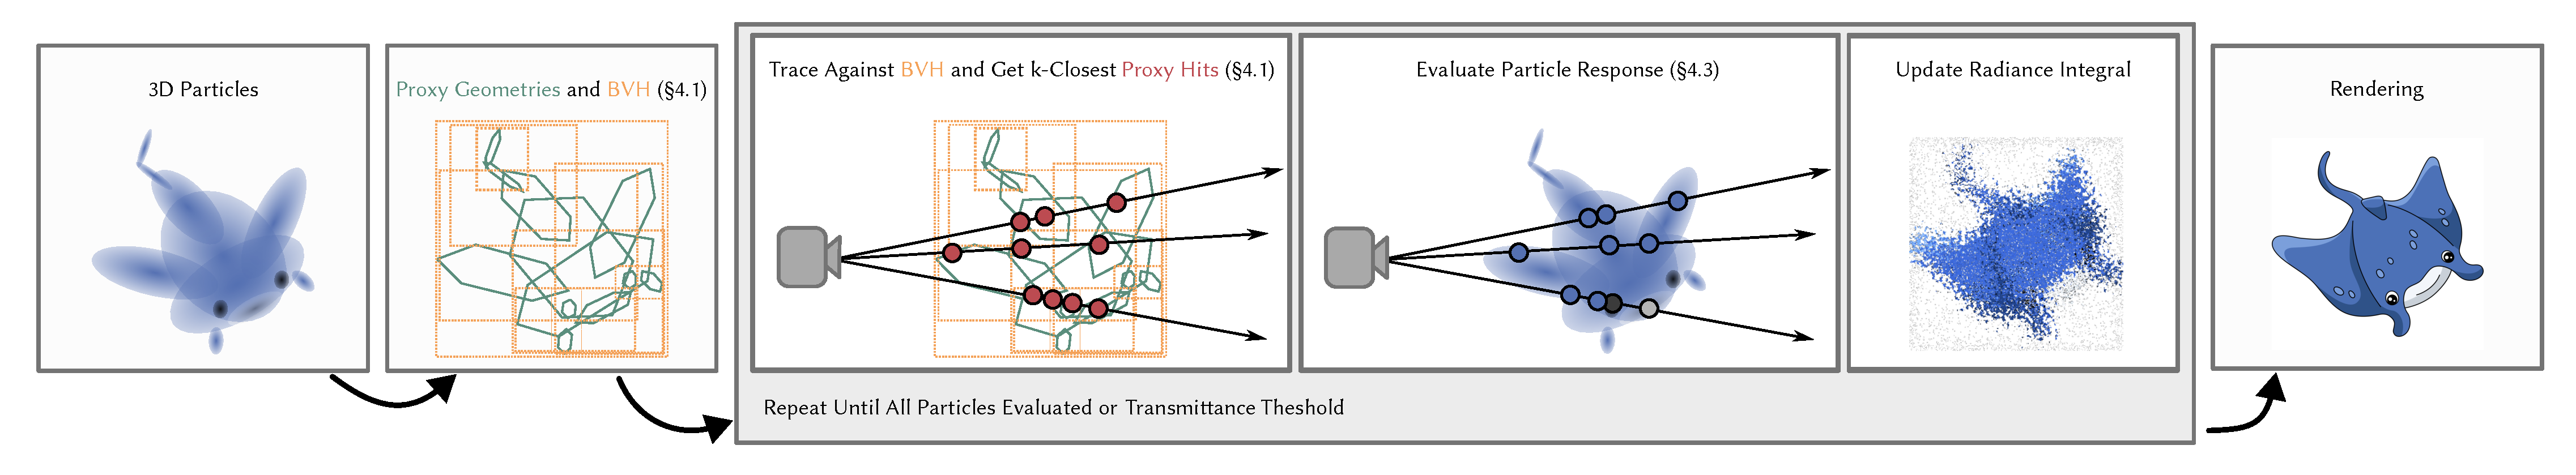
\includegraphics[width=0.92\textwidth]{figures/ch02/2407_07090_method.pdf}
\caption{3DGRT 渲染管线：高斯粒子→代理几何体/BVH→光线追踪求交→评估粒子响应→累积辐射度→渲染输出。图源：Moenne-Loccoz et al.（2024.07）~\cite{2407_07090}。}
\label{fig:02_3dgrt}
\end{figure}

3DGRT 沿用了 3DGS 的高斯 billboards 表示，通过代理几何体将现有基元映射到光线追踪管线——它在渲染管线层面做创新，但未触及基元本身的物理含义。EVER（2024.10）~\cite{2410_01804} 则选择了另一条路：不改变渲染管线，而是从根本上重新定义基元本身的物理含义，并精确求解体渲染方程。EVER 用恒定密度椭球替代高斯衰减，使体渲染方程获得闭合解，从而在不引入任何近似的前提下实现精确渲染。

\textbf{基元表示。}3DGS 的高斯基元被当作 2D billboards 投影后 $\alpha$-合成，存在两个根本问题：（1）当基元的合成顺序改变时颜色会突变（产生 popping 伪影），缺乏 3D 一致性；（2）$\alpha$-混合 将每个基元独立渲染后叠加，隐式假设基元互不重叠。EVER 将每个基元重新定义为\emph{恒定密度椭球}——与 3DGS 一样由位置向量、旋转四元数和缩放向量参数化，但内部密度 $\rho_k$ 为常数（而非高斯衰减），颜色由前两阶球谐函数表示。直觉上，高斯衰减的密度使基元在空间中无限延展且边界模糊，而恒定密度的椭球具有明确的内外之分——椭球内部密度均匀，边界处密度突然降为零。密度通过可优化参数 $\tau_k$ 间接控制：$\rho(\tau_k) = -\ln(1 - 0.99\,\tau_k) / (s_{kx} + s_{ky} + s_{kz})$。其设计逻辑是：分母中的三个缩放分量之和近似椭球的平均直径，使得沿最短轴观察时的峰值不透明度恰好等于 $\tau_k$。这确保了即使椭球被极度拉伸，至少一个视角仍具有非零梯度。

\textbf{精确体渲染。}标准体渲染方程要求沿光线积分密度场与颜色场，其一般形式为 $C = \int_0^\infty c_r(t)\,\sigma_r(t)\,\exp\!\bigl(-\int_0^t \sigma_r(s)\,ds\bigr)\,dt$。这一积分在一般密度场下无法解析求解，3DGS 因此通过将高斯投影为 2D billboards、按深度排序后逐个 $\alpha$-合成来近似。不过，这一近似在基元重叠时引入物理误差。EVER 的核心洞察是一个几何事实：恒定密度椭球与光线的交集是一系列有限区间。想象光线穿透一个均匀密度的椭球——光线进入椭球时密度突然出现，离开时突然消失，在椭球内部密度恒定不变。在每个这样的区间内密度和颜色均为常数，因此体渲染方程存在闭合解。

具体算法如下所述。沿光线找到所有相交椭球的前后表面，按距离排序后依次遍历。遇到第 $k$ 个椭球的\emph{前面}时，将 $\rho_k$ 和 $\rho_k c_k$ 分别加到运行总计 $\mu_i$ 和 $\nu_i$ 上，遇到\emph{后面}时则减去。这使得第 $i$ 个区间的累积密度和颜色分别为 $\mu_i = \sum_{k=1}^i \delta_k \rho_k$ 和 $\nu_i = \frac{1}{\mu_i}\sum_{k=1}^i \delta_k \rho_k c_k$（其中 $\delta_k \in \{+1,-1\}$ 标记前后面）。由于每个区间内密度和颜色恒定，积分具有闭合形式 $\alpha_i = 1 - e^{-\mu_i \Delta t_i}$。最终颜色通过 $\alpha$-合成这些区间得到：$C = \sum_{i=1}^N \alpha_i\,\nu_i\,\prod_{j=1}^{i-1}(1-\alpha_j)$。这一公式与 Max (1995) 的分段常数密度四边形规则完全一致，但在这里分段常数不是近似而是设计选择——因此 EVER 在不引入任何近似误差的前提下实现了精确体渲染。光线-椭球求交通过 NVIDIA OptiX 实现：为每个椭球提供轴对齐包围盒（AABB）构建 BVH，再用稳定的各向同性光线-球体求交算法精炼检测结果。

这一策略选择的意义在于：3DGRT 是在保持原有 3DGS 表示的同时引入光线追踪，EVER 则同时修正了表示的物理含义和渲染方程的求解方式。在 RTX 4090 上，EVER 以约 30 FPS（720p）运行，在 Zip-NeRF 大规模场景上达到实时方法中最锐利的结果。

\paragraph{在光栅化中实现体积一致性。}

EVER 通过光线追踪硬件实现精确体渲染，但硬件依赖限制了其适用范围。Talegaonkar~et~al.（2024.12）~\cite{2412_03378} 证明了另一条路径的可行性：不使用光线追踪硬件，在标准光栅化器内部实现接近 EVER 的物理准确性。两者的核心差异在于：EVER 将每个椭球分解为前后表面，沿光线维护密度和颜色的运行总计 $\tau_i = \sum_{k=1}^{i} \rho_k$，在各段上求解分段常数密度的闭合解 $\alpha_i = 1 - \exp(-\tau_i \Delta t_i)$，需要光线-椭球求交来定位前后表面。而该方法完全不执行 splatting，直接在光线坐标系中解析计算 3D 高斯的体积积分。

直觉上，这种方法的关键步骤是：一个 3D 高斯沿一条特定光线看去，其密度分布恰好也是一个 1D 高斯——就像用一根细针穿过一个三维的高斯云，针上各点的密度恰好形成钟形曲线。具体而言，该方法将第 $j$ 个 3D 高斯 $G_j(\mathbf{x}) = \exp\{-\frac{1}{2}(\mathbf{x}-\boldsymbol{\mu}_j)^\top \boldsymbol{\Sigma}_j^{-1}(\mathbf{x}-\boldsymbol{\mu}_j)\}$ 沿光线 $\mathbf{r}(t) = \mathbf{o} + t\mathbf{d}$ 精确约化为 1D 高斯分布：$g_j(t) = G_j(t_j\mathbf{d})\,\exp\{-\frac{(t-\mu_j)^2}{2\sigma_j^2}\}$，其中均值 $\mu_j = \frac{(\boldsymbol{\mu}_j - \mathbf{o})^\top \boldsymbol{\Sigma}_j^{-1}\mathbf{d}}{\mathbf{d}^\top \boldsymbol{\Sigma}_j^{-1}\mathbf{d}}$，方差 $\sigma_j^2 = \frac{1}{\mathbf{d}^\top \boldsymbol{\Sigma}_j^{-1}\mathbf{d}}$，$G_j(t_j\mathbf{d})$ 是高斯沿光线的峰值密度。对该 1D 高斯在区间 $[t_{jn}, t_{jf}]$ 上积分，得到解析透射率 $T_j = \exp(-G_j(t_j\mathbf{d})\sqrt{2\pi}\,\sigma_j)$，从而精确计算 $\alpha_j = 1 - T_j$。

与 3DGS 的 EWA splatting 相比，3DGS 做了三层近似。(a) 将指数透射率线性化 $e^{-x} \approx 1-x$。(b) 假设高斯不自遮挡（no self-occlusion），导致 2D 不透明度 $\alpha_i = o_i \cdot \tilde{G}_i(\mathbf{p})$ 仅在 2D 高斯中心处达到峰值 1，无法精确表示不透明表面。(c) 用仿射近似（Jacobian 矩阵 $\mathbf{J}$）将 3D 协方差投影为 2D 协方差 $\boldsymbol{\Sigma}' = \mathbf{J}\mathbf{W}\boldsymbol{\Sigma}\mathbf{W}^\top\mathbf{J}^\top$，在远离线性化中心处引入误差。此外，splatting 丢弃了高斯沿相机光线的 $z$ 轴尺度信息，使得渲染对 $z$ 方向的缩放不敏感——而物理上更大的 $z$ 尺度应使高斯更不透明。该方法通过在光线坐标系中直接积分，同时消除了上述三层近似，且保留了 $z$ 轴尺度的物理效应。在假设基元不重叠且正确排序的条件下，该方法最终仍输出与 3DGS 相同的 $\alpha$-混合 公式 $C(\mathbf{p}) = \sum_{i=1}^{N} c_i \alpha_i \prod_{j=1}^{i-1}(1-\alpha_j)$，但 $\alpha_i$ 的计算从近似 splatting 替换为解析积分。在 NeRF-Synthetic 数据集上全面超越 3DGS，同时可直接用于断层扫描重建。

\paragraph{Unscented Transform 统一投影模型。}

上述方法聚焦于渲染方程的精度改进，而 Wu~et~al.（2024.12）~\cite{2412_12507} 提出的 3DGUT（3D Gaussian Unscented Transform）则从投影模型的角度解决 EWA splatting 的根本局限——与其在投影函数上做近似，不如用采样策略绕过线性化。理解其贡献需要先厘清 3DGS 原本的投影机制：3DGS 将世界坐标系下的 3D 高斯（位置 $\boldsymbol{\mu} \in \mathbb{R}^3$，协方差 $\boldsymbol{\Sigma} \in \mathbb{R}^{3 \times 3}$）经由刚体变换 $\boldsymbol{W} \in SE(3)$ 变换到相机坐标系后，通过 EWA splatting 的一阶 Taylor 近似将 3D 协方差投影为 2D 协方差 $\boldsymbol{\Sigma}' = \boldsymbol{J}\boldsymbol{W}_{[:2,:3]}\boldsymbol{\Sigma}\boldsymbol{W}_{[:2,:3]}^\top\boldsymbol{J}^\top$，其中 $\boldsymbol{J} \in \mathbb{R}^{3 \times 3}$ 是投影函数的仿射近似的雅可比矩阵。这一线性化即使在理想针孔相机下也忽略了高阶项，且畸变越大误差越严重。更关键的是，每引入一种新相机模型（如等距鱼眼模型）都需要手动推导对应的 $\boldsymbol{J}$。而滚动快门等时间依赖效应在 EWA 框架内甚至难以表达。

3DGUT 的核心思想是不再线性化投影函数，而是用有限个采样点（称为 sigma 点）近似 3D 高斯分布本身。直觉上，这类似于用少量探针点”刻画“整个高斯云的形状：选取几个有代表性的空间位置，将它们分别投影到 2D 后重新拟合出投影后的 2D 高斯。受 Unscented Kalman Filter（无迹卡尔曼滤波，UKF）启发，对于 $N=3$ 维的 3D 高斯，选取 $2N+1=7$ 个 sigma 点 $\mathcal{X} = \{\chi_i\}_{i=0}^{6}$，利用协方差的 Cholesky 分解 $\boldsymbol{\Sigma} = \boldsymbol{R}^\top\boldsymbol{S}^\top\boldsymbol{S}\boldsymbol{R}$ 读取矩阵平方根：

\begin{align*}
\chi_0 &= \boldsymbol{\mu}, \\
\chi_i &= \boldsymbol{\mu} + (\sqrt{(3+\lambda)})\,\boldsymbol{e}_{[i]}, \quad i=1,2,3, \\
\chi_i &= \boldsymbol{\mu} - (\sqrt{(3+\lambda)})\,\boldsymbol{e}_{[i-3]}, \quad i=4,5,6,
\end{align*}

其中 $\boldsymbol{e}_{[k]}$ 为协方差矩阵平方根的第 $k$ 列，$\lambda = \alpha^2(3+\kappa)-3$ 由超参数 $\alpha$（控制 sigma 点距均值的散布，实验取 $\alpha=0.001$）、$\kappa$（缩放参数，取 $0$）和 $\beta$（分布先验，取 $2$）决定。每个 sigma 点独立通过任意非线性投影函数 $\hat{\chi}_i = g(\chi_i)$ 精确投影到 2D，然后通过加权后验重建 2D 均值和协方差：

\begin{align*}
\boldsymbol{\mu}' &= \sum_{i=0}^{6} w_i^{(m)}\,\hat{\chi}_i, \\
\boldsymbol{\Sigma}' &= \sum_{i=0}^{6} w_i^{(c)}\,(\hat{\chi}_i - \boldsymbol{\mu}')(\hat{\chi}_i - \boldsymbol{\mu}')^\top,
\end{align*}

其中均值权重 $w_0^{(m)} = \lambda/(3+\lambda)$、$w_{i>0}^{(m)} = 1/(2(3+\lambda))$，协方差权重 $w_0^{(c)} = \lambda/(3+\lambda) + (1-\alpha^2+\beta)$、$w_{i>0}^{(c)} = 1/(2(3+\lambda))$。该近似在分布匹配的精度上至少保留了前三阶矩。

这一机制完全绕过了雅可比矩阵的推导，使得 3DGUT 原生支持任意畸变相机模型和滚动快门——后者只需为每个 sigma 点施加不同的外参矩阵即可。KL（Kullback-Leibler）散度评估表明，在静态针孔相机下 UT 与 EWA 的投影精度相当，但在鱼眼相机下 UT 显著优于 EWA。而在滚动快门场景下，EWA 的线性化完全失效，UT 仍能保持稳定的投影精度。同时，3DGUT 将粒子响应评估从 2D 像素空间改为 3D 光线空间（沿光线计算最大响应点），避免了梯度通过投影函数的反向传播。这使其与 3DGRT 的渲染公式对齐——同一场景既可光栅化也可光线追踪，支持反射、折射等二次光线效果。

\subsubsection{无需专用硬件的可微光线追踪}

3DGRT 依赖 NVIDIA OptiX 硬件加速，这限制了其在非 NVIDIA 平台上的可用性。两条路线尝试在不依赖专用光线追踪硬件的情况下实现类似效果。

\paragraph{Govindarajan}
Govindarajan~et~al.（2025.02）~\cite{2502_01157} 提出的 Radiant Foam 是该方向的锚点工作。与 3DGRT 需要 OptiX 硬件加速不同，Radiant Foam 重新发现了一种在计算机视觉研究中长期被忽视的经典高效体积网格光线追踪算法，仅需标准可编程 GPU 特性即可运行，在渲染速度和质量上与 3DGS 相当，同时不受光栅化的近似限制——从而在不牺牲效率的前提下消除了对专用光线追踪硬件的依赖。

\paragraph{Radiant}
Xu~et~al.（2026.03）~\cite{2603_23637} 则采取正交策略。与 Radiant Foam 用经典光线追踪算法替代硬件加速不同，该方法通过随机采样从根本上消除排序需求：对每条光线仅采样少量高斯子集进行评估的无偏 Monte Carlo 估计器，在标准 3DGS 场景中匹配光栅化质量和速度。更重要的是，在可重光照（relightable）3DGS 场景中，同一估计器驱动逐高斯着色和完整光线追踪的阴影光线，无需近似阴影映射，实现了比先前工作明显更高的重建保真度。

\subsubsection{可编辑与矢量化的高斯渲染}

前面的方法主要追求渲染的物理准确性和效率，而另一类工作关注如何让高斯渲染支持场景编辑和更精确的几何表示。

\paragraph{可编辑高斯光线追踪。}

Byrski~et~al.（2025.03）~\cite{2503_12284} 提出的 REdiSplats 是该方向的锚点工作，其核心贡献是将扁平高斯近似为可编辑的正八边形网格，使同一基元同时满足光线追踪求交和用户直接拖拽编辑两个需求。具体而言，3DGRT（2024.07）~\cite{2407_07090} 用拉伸的规则二十面体（20 面）作为代理包围体，每个交叉命中后还需额外计算高斯响应采样点；REdiSplats 则将扁平高斯（$s_1=0$，即 2D 椭圆）直接近似为正八边形网格，交叉点同时确定高斯身份并提供 opacity 计算所需的距离参数，无需第二个采样点。

具体而言，在扁平高斯的局部坐标系（$OY$--$OZ$ 平面）中，八边形的直觉是将圆形高斯截面离散化为正八边形——就像用正八边形近似一个圆，顶点到中心的距离由统计学置信水平决定。第 $i$ 个顶点为
\begin{equation}
  x_i = \Bigl[0,\; \cos\!\Bigl(\tfrac{2\pi i}{8}\Bigr),\; \sin\!\Bigl(\tfrac{2\pi i}{8}\Bigr)\Bigr] \cdot Q, \quad i=0,\ldots,7,
\end{equation}

其中 $Q = F_{\chi^2(3)}^{-1}(\beta)$ 为卡方分布（3 自由度）在置信水平 $\beta$ 下的分位数。全局坐标通过仿射变换 $P_i = RS \cdot x_i + \mu$ 获得，其中 $R=[r_1,r_2,r_3]$ 为旋转矩阵，$S=\mathrm{diag}(0,s_2,s_3)$ 为缩放矩阵。八边形以 triangle fan 形式三角化为中心点 + 8 个外顶点的 6 个三角形，利用 NVIDIA OptiX 的硬件加速 ray-triangle 求交直接检测光线-高斯碰撞。

在编辑方面，用户拖拽网格顶点 $P_i \to P_i'$ 后，REdiSplats 从 8 个顶点中选取 3 个关键点（$I=\{0,2\}$，即间隔 $90^\circ$ 的两个外顶点加中心点）重建高斯参数：首先由 $r_2 = \widehat{P_{i_1}'}$ 恢复第二旋转轴和缩放 $s_2$，再通过一步 Gram-Schmidt 正交化得到 $r_3$ 和 $s_3$，最后 $r_1 = r_2 \times r_3$，$s_1=0$。该重建过程保证无编辑操作时参数恒等，且仅需 3 个自由顶点而非全部 9 个，避免过度编辑破坏八边形的正则结构。

REdiSplats 在光线追踪中支持阴影投射、镜面反射（如玻璃和镜面对象）以及与 mesh 场景的混合渲染，同时网格表示可直接导入 Blender 和 Nvdiffrast 进行物理仿真和手动编辑，首次在单一框架中统一了光线追踪、场景编辑和物理仿真。

\paragraph{矢量图元混合表示。}

REdiSplats 通过将扁平高斯近似为三角化八边形网格实现了可编辑性，但其基元仍本质上是高斯的——高斯核固有的空间无限延展导致边界模糊。Wu~et~al.（2025.03）~\cite{2503_13961} 提出的 BG-Triangle（B\'{e}zier Gaussian Triangle）选择了一条更根本的路线：在确定性（贝塞尔三角形矢量图元）和概率性（高斯核）两个极端之间建立混合表示，用贝塞尔三角形的精确边界解决高斯核的模糊问题，同时用高斯子基元保留可微渲染能力。

直觉上，B\'{e}zier 三角形与 CAD 软件中常用的贝塞尔曲面片类似：控制点定义了一个光滑的三角形曲面片，边界由重心坐标严格限定——重心坐标 $(u,v,w)$ 在三角形内部为正，在边界上为零，在三角形外部为负，因此 $u+v+w=1$ 且 $u,v,w \geq 0$ 恰好定义了三角形的闭合区域。具体而言，BG-Triangle 的几何基元是 $n$ 次 B\'{e}zier 三角形曲面 $S$，由控制点 $p_{i,j,k} \in \mathbb{R}^3$（其中 $i+j+k=n$, $i,j,k \geq 0$）定义，参数化形式为：

\begin{equation}
S(u,v,w) = \sum_{i=0}^{n} \sum_{j=0}^{n-i} B_{i,j,k}^{n}(u,v,w) \, p_{i,j,k}
\end{equation}

其中 $B_{i,j,k}^{n}(u,v,w) = \frac{n!}{i!\,j!\,k!} u^i v^j w^k$ 为 Bernstein 多项式。这一参数化与 REdiSplats 的本质区别在于：REdiSplats 用三角化八边形近似扁平高斯的置信椭球，顶点由高斯参数刚性导出，几何仍是高斯的离散化；而 BG-Triangle 的控制点通过 Bernstein 插值生成连续曲面，天然具有精确边界——重心坐标域 $u+v+w=1$ 严格定义了基元的闭合边界，不存在高斯核的空间无限延展问题。

然而，仅有确定性几何无法实现可微渲染——几何提供精确边界但无法生成平滑的梯度信号。BG-Triangle 的核心设计在于双层表示的协同：几何层（B\'{e}zier 三角形）定义精确边界和表面位置，外观层（高斯子基元）在每个像素位置”按需“生成，提供可微的颜色和属性插值。

渲染管线首先将 B\'{e}zier 三角形细化为扁平三角面片，经传统光栅化生成坐标图 $I_{uv} \in \mathbb{R}^{H \times W \times 3}$ 和索引图 $I_{id} \in \mathbb{Z}^{H \times W}$，为每个像素记录其所属基元的重心坐标和 ID。随后，在每个前景像素 $q$ 处根据重心坐标计算 3D 位置 $S_q$，并在该位置动态生成高斯子基元（sub-primitive）。这些子基元继承旋转、缩放和球谐系数等属性，但不包含不透明度——因为几何已由 B\'{e}zier 三角形定义。属性插值分为两类：漫反射颜色通过颜色控制点 $p_{i,j,k}^c$ 经 Bernstein 插值计算 $c_q = \sum_{i,j} B_{i,j,k}^n(I_{uv}(q)) \, p_{i,j,k}^c$；旋转、缩放和 SH 系数则通过基于重心坐标的多分辨率 2D 属性图 $M_h$ 进行纹理插值。这种”on-the-fly“生成策略意味着不同视角使用不同的高斯集合，但均从同一组 B\'{e}zier 控制点采样，确保了几何一致性。

上述结构在每个 BG-Triangle 内部保证了平滑过渡，但基元边界处的高斯不确定性仍会导致模糊。直接在边界截断高斯会破坏可微性——梯度会在截断处断裂。因此 BG-Triangle 引入不连续感知 $\alpha$-混合（discontinuity-aware $\alpha$-混合）机制：在基元边界处用一个平滑过渡函数逐渐降低 alpha 值，而非突然截断。首先，光栅化阶段检测相邻像素归属不同基元 ID 的边界像素，构成 2D 边界点集 $\mathcal{B}$，并通过 B\'{e}zier 映射反投影为 3D 边界点。每个边界点被建模为固定缩放因子 $r_b$ 的各向同性高斯，其投影半径 $\delta_i$ 定义了影响范围。直觉上，距离边界越远的像素受边界过渡函数的影响越小（保持原值），距离边界越近的像素则被平滑地抑制——这就像在两个不同颜色的区域之间画一条渐变带。对于光栅化高斯 $G$ 覆盖的像素 $q$，混合系数定义为：

\begin{equation}
w(q) = \begin{cases} 0, & I_{id}(b_i) \neq g \\ g(\|q - b_i\|_2; \delta_i), & I_{id}(b_i) = I_{id}(q) \\ 1 - g(\|q - b_i\|_2; \delta_i), & \text{otherwise} \end{cases}
\end{equation}

其中 $g$ 为高斯 $G$ 所属基元的 ID，模糊函数 $g(d;\delta) = \sigma(2^{d/\delta-1}, 1)$ 将距离 $d$ 映射到 $[0.5, 1.0]$，使 $w(q)$ 在边界区域内从 $1.0$ 平滑过渡到 $0.0$。修正后的 alpha 值为 $\alpha'(q) = o \cdot w(q) \cdot e^{-\frac{1}{2}(q-\boldsymbol{\mu})^\top \boldsymbol{\Sigma}^{-1}(q-\boldsymbol{\mu})}$，其中 $o \approx 1.0$ 为常数。在训练优化方面，BG-Triangle 采用基于控制点梯度幅度和训练视图边缘先验的双重分裂准则：梯度范数超过 $\lambda_g$ 的基元或累积边缘梯度超过 $\lambda_b$ 的基元被分裂以拟合细节；同时基于可见性、面积和纵横比三个标准修剪无效基元。通过这一确定性几何与概率性外观的混合表示，BG-Triangle 使用远少于 3DGS 的基元达到可比渲染质量，同时在边界保持方面显著优于 3DGS 和 NeRF。

\subsubsection{科学可视化与跨模态应用}

3DGS 的光线追踪能力不仅限于视觉渲染，还可服务于科学计算和跨模态仿真，这一扩展从三个方向展开。

\paragraph{Sharma et al.：科学体渲染 LOD 近似}
\textbf{科学体渲染}。Sharma~et~al.（2025.04）~\cite{2504_04857} 将 3DGS 的光线追踪思想应用于科学可视化领域，利用 3D 高斯粒子在不同 LOD 下近似 VDB 体素数据，是该方向的首个工作。

\paragraph{GSCache：多级路径空间辐射缓存}
Bauer~et~al.（2025.07）~\cite{2507_19718} 提出的 GSCache 则将 3DGS 适配为多级路径空间辐射缓存，利用高效光栅化器加速体渲染中的路径追踪，支持在线训练动态适应光照配置和传输函数变化——与 Sharma~et~al. 的静态 LOD 近似不同，GSCache 侧重于动态路径追踪的高效缓存策略。

\paragraph{Kohyama}
\textbf{事件驱动渲染}。从科学体渲染的连续场近似转向另一种模态，Kohyama~et~al.（2025.12）~\cite{2512_18640} 提出的 GPERT 将事件相机的逐事件稀疏特性与光线追踪结合：将渲染解耦为逐事件几何渲染和快照式辐射渲染两个分支，这是首个事件驱动的 3DGS 光线追踪框架。

\paragraph{Vaara et al.：可微分射频传播仿真}
\textbf{跨模态电磁仿真与硬件优化}。从视觉波段扩展到电磁频谱，Vaara~et~al.（2026.05）~\cite{2605_07781} 提出将 Gaussian 基元嵌入光线追踪结构，首次实现可微分射频传播仿真，证明神经重建可同时服务于电磁仿真和光真实感渲染。

\paragraph{GRTX：光线追踪管线效率优化}
Lee~et~al.（2026.01）~\cite{2601_20429} 提出的 GRTX 则从软硬件协同角度优化高斯基光线追踪，通过光线空间变换将各向异性高斯视为单位球以减少 BVH 开销，引入遍历检查点机制消除冗余节点访问——与 Vaara~et~al. 的应用驱动路线互补，GRTX 聚焦于底层管线效率优化。

\paragraph{Stekovic}
此外，Stekovic~et~al.（2024.04）~\cite{2404_10620} 提出的 PyTorchGeoNodes 将 Blender 中的程序模型解析为可微 PyTorch 代码，利用遗传算法与梯度优化的组合策略同时优化离散和连续参数，展示了与 3DGS 集成实现程序化高斯泼溅的可能性。

\paragraph{光栅化与光线追踪的融合趋势}
总的来说，从光栅化到光线追踪的转变代表了 3DGS 渲染能力的质变。3DGRT（2024.07）~\cite{2407_07090} 和 EVER（2024.10）~\cite{2410_01804} 从两个方向证明：在 3DGS 的粒子场景中，光线追踪可以达到与光栅化相当的效率。

\paragraph{3DGUT 与体渲染一致性}
3DGUT（2024.12）~\cite{2412_12507} 和 Volumetrically Consistent Rasterization（2024.12）~\cite{2412_03378} 则证明在光栅化框架内也可以实现更物理准确的体渲染。

\paragraph{随机光线追踪效率提升}
随机光线追踪（2026.03）~\cite{2603_23637} 通过消除排序开销进一步提升了效率。这些工作共同指向一个趋势：3DGS 的渲染管线正在从纯光栅化向混合渲染（光栅化 + 光线追踪）演进，以兼顾效率和物理准确性。

\begin{takeaway}
3DGS 的渲染管线正在从纯光栅化向混合渲染演进。3DGRT 和 EVER 等工作通过 BVH 光线追踪实现阴影、反射等物理效果，3DGUT 则在光栅化框架内实现了更物理准确的体渲染。这一方向的核心权衡是光线追踪带来的物理准确性提升与排序开销增加之间的平衡。
\end{takeaway}

% ============================================================
% 第2章 中间部分：2.6--2.8
% ============================================================

\subsection{近期方法脉络：射线查询与高级渲染、Fast ray tracing for 3D Gaussians}

这一组近期工作延续 3DGS rasterization、3D Gaussian Ray Tracing，主要把改动集中在扩展、加速等环节。下面只保留相对既有路线的变化，便于和前文方法直接对照。

\paragraph{Directed Distance Fields for Constant-Time Ray Queries on Gaussian Splatting}
Directed Distance Fields for Constant-Time Ray Queries on Gaussian Splatting（2026.05）~\cite{2606_00817} 延续 3DGS rasterization 在“射线查询与高级渲染”上的基本设定，主要改变是：从3DGS蒸馏Directed Distance Field，将射线映射到首个表面距离和命中状态，实现常数时间ray oracle。高斯基元表示仍作为基础。
其设计动机是：提出从3DGS训练小型DDF神经场的方法，使查询成本与高斯数量无关，为3DGS补足传统光栅化难以处理的secondary rays能力。
具体而言，DDF输入射线起点和方向，输出首交距离和命中概率；论文比较深度监督和干净距离监督，发现后者更能恢复薄结构。
适用边界是：需要额外蒸馏训练；距离监督质量影响薄结构；DDF是辅助神经场而非直接改造高斯表示。

\paragraph{GRay}
GRay（2026.06）~\cite{2606_30869} 可作为“Fast ray tracing for 3D Gaussians”中的新锚点候选。相较于 3D Gaussian Ray Tracing，主要改变是：只评估被光线相交的 Gaussians，并优化 3D Gaussian ray tracing 管线。高斯基元表示仍作为基础。
其设计动机是：利用 ray tracing 与 rasterization 的算法差异，避免评估所有投影相关 splats，而只处理实际相交的 Gaussians。
具体而言，设计面向 3D Gaussians 的高效 ray tracing 方法，通过加速结构和相交评估降低 3DGRT 近一个数量级的优化开销。
这一锚点判断来自当前分类中的机制关系：候选锚点：加速，且相关性 0.95；后续方法可围绕 为 3D Gaussians 设计接近 splatting 速度的 ray tracing 渲染器。 继续比较和扩展。
适用边界是：ray tracing 管线复杂度和硬件适配仍需考虑；透明混合和梯度稳定性可能是关键实现细节。
\section{渲染管线与排序优化}
\label{sec:02_6}

3DGS 的渲染效率建立在一个核心设计设定之上：tile-based 光栅化配合基于深度排序的 $\alpha$-混合。原始 3DGS 将图像平面划分为 $16\times16$ 像素的 tile，对每个 tile 内的高斯基元按视图空间 $z$ 坐标执行全局排序（radix sort），然后从前到后执行 $\alpha$-混合 计算像素颜色。这一设定带来了三方面的问题。(1) 排序本身是计算瓶颈，尤其在基元数量达到百万级别时开销显著。(2) 全局排序按基元中心深度进行，无法保证逐像素的正确深度顺序，导致视角旋转时出现”弹出“（popping）伪影。(3) 仿射投影近似在大视场角和近距离观察时引入几何失真。围绕这些问题，研究者从排序策略、混合公式和渲染管线结构三个维度展开了系统性优化。图~\ref{fig:02_pipeline_opt} 展示了三层优化策略。

\begin{figure}[htbp]
\centering
\resizebox{0.85\textwidth}{!}{\begin{tikzpicture}[
  layer/.style={rectangle, rounded corners=6pt, draw=#1, fill=#1!8,
    text width=13cm, minimum height=1.5cm, align=left, font=\small},
  mname/.style={font=\scriptsize\ttfamily, techgray},
  arr/.style={-{Stealth[length=6pt]}, very thick, techgray},
  >=Stealth
]
  % Layer 3 (底部): 管线效率优化
  \node[layer=techpurple] (l3) at (0, 0) {%
    \textbf{Layer 3: 管线效率优化}%
    \hfill {\scriptsize 减少冗余计算 + 利用硬件特性}%
  };
  \node[mname, anchor=north west] at ([xshift=0.3cm, yshift=-0.1cm]l3.north west) {
    FlashGS \textbullet{} Speedy-Splat \textbullet{} QuadBox \textbullet{} TC-GS \textbullet{} TensorGS \textbullet{} GEMM-GS
  };

  % Layer 2 (中部): 排序精度改进
  \node[layer=techorange] (l2) at (0, 2.3) {%
    \textbf{Layer 2: 排序精度改进}%
    \hfill {\scriptsize 逐像素精确排序 + 投影校正}%
  };
  \node[mname, anchor=north west] at ([xshift=0.3cm, yshift=-0.1cm]l2.north west) {
    StopThePop \textbullet{} Plucker坐标 \textbullet{} 混合透明度 \textbullet{} 精确椭球投影
  };

  % Layer 1 (顶部): 消除排序依赖
  \node[layer=techblue] (l1) at (0, 4.6) {%
    \textbf{Layer 1: 消除排序依赖}%
    \hfill {\scriptsize 可交换混合替代 alpha blending}%
  };
  \node[mname, anchor=north west] at ([xshift=0.3cm, yshift=-0.1cm]l1.north west) {
    WSR (加权求和) \textbullet{} StochasticSplats \textbullet{} Duplex-GS \textbullet{} MB3DGS
  };

  % 层间箭头
  \draw[arr] (l1.south) -- (l2.north) node[midway, right=0.3cm, font=\scriptsize, techgray] {排序仍然需要};
  \draw[arr] (l2.south) -- (l3.north) node[midway, right=0.3cm, font=\scriptsize, techgray] {排序已优化};

  % 右侧标注：效果
  \node[font=\scriptsize, techblue, anchor=west] at (7, 4.6) {弹出伪影 = 0};
  \node[font=\scriptsize, techorange, anchor=west] at (7, 2.3) {高斯减少 50\%};
  \node[font=\scriptsize, techpurple, anchor=west] at (7, 0) {渲染加速 1.5--7$\times$};
\end{tikzpicture}
}
\caption{渲染管线优化的三层策略。Layer~1 从根本上消除排序需求，Layer~2 提升排序精度，Layer~3 优化管线效率。三层可叠加使用。}
\label{fig:02_pipeline_opt}
\end{figure}

\subsection{消除排序依赖：顺序无关渲染}

排序是 3DGS 渲染管线中计算量最大的环节之一。
一系列工作试图从根本上消除对排序的需求，转而采用可交换的混合操作替代非交换的 $\alpha$-混合。
这些方法沿着从”可交换近似“到”无偏物理建模“再到”理论重构“的路径逐步演进。

\subsubsection{顺序无关渲染方法}

\paragraph{Hou}
Hou~et~al.（2024.10）~\cite{2410_18931} 提出的 Weighted Sum Rendering（WSR）是该方向的奠基性工作。
其核心思路直观而激进：既然排序的根源在于 $\alpha$-混合 的非交换性（先渲染红再渲染蓝，与反过来结果不同），那么如果用一种\emph{与顺序无关}的混合公式替代 $\alpha$-混合，排序自然就不再需要。
具体而言，WSR 将颜色混合视为对高斯颜色的深度加权平均——越靠近相机的高斯权重越大——这一操作天然与求和顺序无关。
其混合公式为：

\begin{equation}
C = \frac{c_B w_B + \sum_{i=1}^{N} c_i \alpha_i w(d_i)}{w_B + \sum_{i=1}^{N} \alpha_i w(d_i)}
\end{equation}

其中 $c_B$ 和 $w_B$ 为背景的颜色和可学习权重，$d_i$ 为第 $i$ 个高斯的深度，$w(\cdot)$ 为可学习的权重函数。
由于求和天然具有交换性，渲染过程完全无需排序即可并行执行，同时消除了排序变化引起的时序弹出伪影。

权重函数 $w(d_i)$ 的设计是 WSR 的核心，论文提出三种变体，精度逐步提升。

\textbf{DIR-WSR}（Direct）使用常数权重 $w(d_i) = 1$，完全忽略深度信息，由网络通过调整不透明度 $\alpha_i$ 来补偿。
然而，当两个不透明高斯（$\alpha = 1$）颜色不同时，DIR-WSR 始终输出两色的混合色（如红蓝混合为紫色），无法正确建模遮挡关系，在复杂场景中引入明显的模糊伪影。

\textbf{EXP-WSR}（Exponential）引入深度依赖的指数权重 $w(d_i) = e^{-\lambda d_i^\beta}$，其中 $\lambda, \beta$ 为可学习参数（训练时分别初始化为 $0.1$ 和 $0.8$），使靠近相机的高斯获得更大权重以近似遮挡效果。
但远处高斯的权重虽衰减却永不为零，仍然贡献残余颜色，导致在密集重叠区域产生视觉失真。

\textbf{LC-WSR}（Linear Correction）受可变形卷积和 KPConv 启发，采用线性修正权重 $w(d_i) = \max(0,\, 1 - \lambda d_i) \cdot v_i$，其中 $\lambda$（初始化为 $10$）和 $v_i$（初始化为 $0.1$）为可学习参数。
与 EXP-WSR 的关键区别在于：LC-WSR 可以将远处高斯的权重精确降至零，彻底消除其对渲染的贡献，从而更准确地建模硬遮挡边界，且计算开销低于 EXP-WSR。

除权重函数外，WSR 还将原始 3DGS 中固定的最大不透明度 $t_i$ 替换为视角依赖的不透明度 $u_i = Y(\|\mathbf{d}_i\|, \mathbf{H}_i)$，其中 $Y(\cdot)$ 为球谐函数，$\mathbf{H}_i$ 为可学习的球谐系数向量。
这一机制使同一高斯从不同视角观察时具有不同的不透明度，部分弥补了 WSR 缺少排序所丢失的遮挡信息。
值得注意的是，$u_i$ 不再像原始 3DGS 那样被裁剪到 $[0,1]$ 区间，赋予了网络更大的表达自由度。
训练过程中，WSR 使用与原始 3DGS 完全相同的 $\mathcal{L}_1$ + D-SSIM 损失函数（D-SSIM 权重因子 $0.2$），但优化对象从固定不透明度参数变为权重函数参数和视角依赖不透明度的球谐系数。

WSR 在物理上牺牲了体渲染方程的严格闭合解，换来了对排序的完全独立。在移动设备 GPU 上实现平均 1.23 倍渲染加速，且特别适合 WebGL/Vulkan 等无法高效执行全局排序的平台。其核心局限在于：即使是最精确的 LC-WSR 变体，加权求和仍然是一种近似混合，无法在半透明物体密集重叠的场景中完全复现 $\alpha$-混合 的物理正确结果。
沿”消除排序但提升物理准确性“的方向，后续工作分别从统计采样、双层次框架、矩方法和理论重构四个角度改进。

\paragraph{统计采样路线。}
针对 $\alpha$-混合 公式本质上是加权期望值、而任何期望都可用蒙特卡洛采样无偏估计的观察，StochasticSplats 将体渲染方程从确定性的排序混合转化为无偏的蒙特卡洛估计，用概率论证明排序只是充分条件而非必要条件，核心思想是\textbf{``混合即期望，采样即求解''}——从而在根本上消除 3DGS 对全局排序的依赖。Kheradmand~et~al.（2025.03）~\cite{2503_24366} 提出的 StochasticSplats 走了一条与 WSR 完全不同的路线：WSR 用可交换的加权求和替换了混合公式，而 StochasticSplats 则保留原始 $\alpha$-混合 公式不变，但通过\textbf{随机采样}来绕过排序需求。
直觉上，$\alpha$-混合 输出的颜色是一个加权期望，而任何期望都可以用蒙特卡洛采样来估计——如果按正确概率随机抽取一个高斯，它的颜色就是无偏的颜色估计。
具体而言，StochasticSplats 将 $\alpha$-混合 公式 $C = \sum_{i=1}^{L} c_i\,\alpha_i \prod_{z_k < z_i}(1-\alpha_k)$ 转化为蒙特卡洛估计问题。
核心思想是按照概率质量函数 $P(i) = \alpha_i \prod_{z_k < z_i}(1-\alpha_k)$ 随机选取一个高斯 $i$，然后通过重要性采样得到无偏估计 $\hat{C} = c_i / P(i) = c_i$——由于 $1/P(i)$ 恰好消去了 $\alpha$-混合 中的透射率项，单次采样只需返回被选中的高斯颜色 $c_i$。
在 GPU 上，这一过程通过标准深度测试实现：为每个像素采样均匀随机数 $u \sim U(0,1)$，在 fragment shader 中测试 $u < \alpha_i$，不满足则 \texttt{discard}——硬件深度测试自动保证被保留的片段是最近（$z$ 最小）的那个，无需全局排序。
最终像素颜色为 $S$ 组独立样本的平均 $\bar{C} = \frac{1}{S}\sum_{s=1}^{S} c_{i_s}$，调整每像素样本数（SPP）即可灵活权衡渲染速度与视觉质量：1 SPP 下比原始 CUDA 3DGS 快 4 倍以上，增大 SPP 则逐步逼近排序 $\alpha$-混合 的 PSNR。

为保证训练中的梯度正确回传，StochasticSplats 借鉴 path replay backpropagation（2021）~\cite{Vicini2021PathReplay}，采用\textbf{分离梯度估计器}（detached gradient estimator）和三遍渲染策略：
（1）第一遍渲染图像并计算损失梯度 $\partial\mathcal{L}/\partial C$；
（2）第二遍使用不同随机种子渲染去相关图像，获取被采样高斯的颜色 $c_i$；
（3）第三遍以与第二遍相同的随机种子重放，利用存储的 $c_i$ 计算参数梯度——其中颜色梯度仅传递给被采样的第 $i$ 个高斯 $\partial\mathcal{L}/\partial c_i = (\partial\mathcal{L}/\partial C)$，不透明度梯度则传递给第 $i$ 个高斯及其前方所有高斯，后方高斯梯度为零。
为避免损失函数两个噪声项的相关性导致梯度偏差，第二遍使用独立随机种子渲染去相关图像，使 L2 损失获得无偏梯度。

在消除 popping 伪影方面，StochasticSplats 提供两个层次。

快速模式下，将 billboard 平面定向为线性逼近高斯最大密度面，平面法向量取 $\mathbf{n} = \boldsymbol{\Sigma}^{-1}(\boldsymbol{\mu} - \mathbf{o})$（$\boldsymbol{\mu}$ 为高斯均值，$\mathbf{o}$ 为相机中心，$\boldsymbol{\Sigma}$ 为协方差矩阵），利用硬件光栅化器的插值内核自动计算 splat 深度，不增加额外开销。

高保真模式下，用 free-flight distance sampling（一种体积渲染中的经典距离采样方法，沿射线随机选取与下一个散射介质”碰撞“的距离）实现完全体积混合——将每个高斯的不透明度重新参数化为空间变化的消光函数 $\sigma_i(\mathbf{p}) = \sigma_t\,\exp\!\bigl(-\tfrac{1}{2}(\mathbf{p}-\boldsymbol{\mu})^T\boldsymbol{\Sigma}^{-1}(\mathbf{p}-\boldsymbol{\mu})\bigr)$，通过解析逆 CDF 采样自由飞行距离 $t$，多个重叠高斯采用 decomposition tracking（分解追踪，取各介质自由飞行距离的最小值来确定最近碰撞）无需额外数据结构或光线追踪即可准确解析任意数量的高斯重叠。

\paragraph{双层次框架路线。}
WSR 和 StochasticSplats 分别通过近似混合和统计采样消除了排序，但都未充分利用 3DGS 渲染的空间局部性。
Liu~et~al.（2025.08）~\cite{2508_03180} 提出的 Duplex-GS 在 WSR 的基础上引入双层次框架，同时解决了 WSR 的透明伪影和传统 $\alpha$-混合 的弹出伪影。

\textbf{第一层：Cell Proxy。}
与 Scaffold-GS 和 Octree-GS 中仅作为抽象编码代理的锚点（anchor）不同，Duplex-GS 引入具有显式几何结构的椭球单元（ellipsoidal cell）作为代理。
每个 cell 由位置 $\boldsymbol{\mu}_n$、尺度 $\mathbf{s}_n$、四元数 $\mathbf{q}_n$ 定义其可见区域，并关联一个潜在特征向量 $\mathbf{f}_n$ 编码局部场景信息。
每个 cell 发射 $K$ 个神经高斯，其颜色 $\mathbf{c}_{n,k}$、尺度比 $O_{n,k}^{\mathrm{scale}}$ 和四元数 $\mathbf{q}_{n,k}$ 由共享的场景级 MLP 从 $\mathbf{f}_n$、视距 $d_n$ 和视角 $\mathbf{d}_n$ 解码得到：
$\{\mathbf{c}_{n,1},\ldots,\mathbf{c}_{n,K}\} = F_c(\mathbf{f}_n, d_n, \mathbf{d}_n)$，$\{O_{n,k}^{\mathrm{scale}},\ldots\} = F_s(\mathbf{f}_n, d_n, \mathbf{d}_n)$。
为使高斯中心严格落在 cell 可见区域内，偏移参数 $O_{n,k}^{\mathrm{pos}}$ 被约束在 $[-1,1]$ 范围内。
高斯尺度由 cell 尺度乘以 sigmoid 激活的尺度比得出：$\mathbf{s}_{n,k} = O_{n,k}^{\mathrm{scale}} \cdot \mathbf{s}_n$，并进一步裁剪 $O_{n,k}^{\mathrm{scale}} = \min(O_{n,k}^{\mathrm{scale}}, 1 - \|O_{n,k}^{\mathrm{pos}}\|)$，确保高斯区域完全包含在 cell 内。
Cell 的四元数通过其关联高斯的加权平均更新：$\mathbf{q}_n = (\sum_k^K \alpha_{n,k} \cdot \mathbf{q}_{n,k}) / \sum_k^K \alpha_{n,k}$。

基于 cell 的显式几何，Duplex-GS 将光栅化从逐高斯操作提升到逐 cell 层面。
仅与视锥相交的 cell 被选中并解码为神经高斯；在 tile-based 范式下，可见 cell 被分配到对应 tile 并对 cell 序列执行基数排序。
由于 cell 数量比高斯少数个数量级，这一策略大幅降低了基数排序的序列长度和内存消耗——排序开销减少 52.2\%--86.9\%。

\textbf{第二层：物理加权求和渲染。}
Duplex-GS 的混合公式建立在 cell 级排序获得的粗粒度深度顺序之上。
它将每个 cell 视为一个整体，定义 cell 权重 $w_n = v_n T_n^{\mathrm{cell}}$，其中 $T_n^{\mathrm{cell}}$ 为 cell 级透射率，按前到后顺序累积衰减：

\begin{equation}
T_n^{\mathrm{cell}} = \prod_{i=1}^{n-1}\prod_{k=1}^{K}(1 - v_i \alpha_{i,k})
\end{equation}

其中 $\alpha_{i,k}$ 为高斯核加权的不透明度，约束在 $[0,1]$ 物理合理范围内（区别于 WSR 中经常超过 1 的无约束权重）；$v_i$ 为可学习的标定标量，用球谐系数参数化以捕捉视角依赖的方向变化，用于补偿 cell 间非均匀空间分布和重叠带来的歧义。
最终渲染颜色为：

\begin{equation}
C = \frac{\sum_{n=1}^{N} w_n \sum_{k=1}^{K} \alpha_{n,k} \mathbf{c}_{n,k}}{\sum_{n=1}^{N} w_n \sum_{k=1}^{K} \alpha_{n,k}}
\end{equation}

这一设计的核心洞察是：\textbf{cell 间有序、cell 内无序}。
Cell 级透射率 $T_n^{\mathrm{cell}}$ 按 cell 深度顺序严格递减，重建了类似 $\alpha$-混合 的物理透射率衰减曲线——当遇到不透明表面时快速衰减至零，从而消除 WSR 中半透明物体消失的失真问题。
而 cell 内部的高斯无需排序，渲染结果局部独立于高斯顺序，因此完全消除了 popping 伪影。

\textbf{早期终止与优化策略。}
由于 $T_n^{\mathrm{cell}}$ 具有物理意义且严格递减，当其降至预设阈值 $\epsilon$ 以下时即可安全终止混合过程——与 vanilla 3DGS 使用相同的阈值参数。
这一机制是此前 WSR 方法所不具备的，因为 WSR 的权重缺乏物理约束，无法支持早期终止。
在优化方面，Duplex-GS 引入三项工程策略：（1）False Positive Skip——通过轴对齐包围盒（AABB）检查剔除像素级冗余高斯核计算；（2）几何校正——定期将 cell 中心更新为其关联高斯中心的均值，确保空间对齐；（3）Cell Position Reset——密度控制新增 cell 后，将显著高斯的偏移重置为零以解耦新旧 cell。
损失函数在原始 $\mathcal{L}_1$ + D-SSIM（权重 $0.2$）基础上额外加入 LPIPS 感知损失（权重 $0.5$，每 20 次迭代计算一次以控制训练开销）。

实验表明，Duplex-GS 比现有基于 OIT 的 3DGS 方法快 1.5--4 倍，在 Mip-NeRF 360 上以 184 FPS 达到最高 PSNR，在中端 RTX 3060 笔记本 GPU 上同样保持最高渲染速度和竞争力视觉质量。

\paragraph{解析矩方法路线。}
Duplex-GS 通过工程策略平衡了 WSR 和精确排序之间的取舍，而 M\"uller~et~al.（2025.12）~\cite{2512_11800} 提出的 Moment-Based 3DGS（MB3DGS）则从物理建模层面提供了更为精细的解决方案。
MB3DGS 的核心思想可以用一个类比理解：与其逐个高斯地按深度排序混合，不如先统计出射线上所有高斯的“深度分布摘要”，再从这个摘要中直接解析透射率——这个“摘要”就是矩（moments）。
与前三者不同，MB3DGS 不依赖任何近似混合公式或统计采样，而是从体渲染方程出发，将沿射线的密度重新参数化为 1D 高斯之和 $\rho(t) = \sum_i \alpha_i \exp\!\bigl(-{(t - \mu_i)^2}/(2\sigma_i^2)\bigr)$，进而计算该密度分布的\textbf{幂矩}（power moments）$m_k = \sum_i \int_{t_n}^{t_f} \varphi(t)^k\,\rho_i(t)\,\mathrm{d}t$（$k = 0, 1, \ldots, 2n$，取 $n = 4$），每个像素仅存储 $2n\!+\!1 = 9$ 个矩即可编码全部高斯的深度分布信息——直觉上，零阶矩编码总不透明度，一阶矩编码平均深度，高阶矩编码分布的展宽和偏度。
为解决远距离高斯矩值呈 $\mu^k$ 指数增长导致的数值不稳定性，MB3DGS 引入 Power-Transform 幂变换 $\varphi(t) = (f(t) - f(t_n))/(f(t_f) - f(t_n))$ 将射线域 $[t_n, t_f]$ 映射到 $[0,1]$，其中 $f(t)$ 设为参数化幂函数 $f_{-1.5}(2t)$，对近距离线性、对远距离呈逆映射，兼顾浮点精度与线性化误差。
在计算每个高斯对矩的贡献 $(m_k)_i$ 时，MB3DGS 在高斯均值 $\mu_i$ 处对 $\varphi(t)$ 做一阶 Taylor 展开，推导出闭合递推关系：零阶矩 $(m_0)_i = \sqrt{2\pi}\,\alpha_i\sigma_i(1 - \mathrm{erf}(b_n))$（$b_n = (t_n - \mu_i)/(\sqrt{2}\sigma_i)$），一阶矩 $(m_1)_i = \varphi(\mu_i)(m_0)_i - \varphi'(\mu_i)\sqrt{2\pi}\sigma_i^2 e^{-b_n^2}$，$k \geq 2$ 阶通过递推 $(m_k)_i = \varphi(\mu_i)(m_{k-1})_i + \varphi'(\mu_i)^2\sigma_i^2(k\!-\!1)(m_{k-2})_i - B_i(k)$ 计算，其中边界修正项 $B_i(k) = -\varphi'(\mu_i)\sqrt{2\pi}\sigma_i^2 u_n^{k-1} e^{-b_n^2}$ 处理近裁剪面的截断效应。

除幂矩外，论文还提出三角矩 $\mu_k = \sum_j \int_{t_n}^{t_f} \bigl(e^{(2-\pi)i\varphi(t)}\bigr)^k \rho_j(t)\,\mathrm{d}t$（$i$ 为虚数单位），同样通过 Taylor 展开得到闭合形式 $(\mu_k)_j \approx \sqrt{2\pi}\alpha_j\sigma_j e^{i k(2-\pi)\varphi(\mu_j) - k^2(2-\pi)^2\varphi'(\mu_j)^2\sigma_j^2/2}(1 - \mathrm{erf}(v_n))$，其中复数变元 $v_n = (t_n - \mu_j)/(\sqrt{2}\sigma_j) - ik(2-\pi)\varphi'(\mu_j)\sigma_j/\sqrt{2}$ 通过一阶 Taylor 展开近似。

矩收集完成后，MB3DGS 利用矩重构透射率的上下界。
具体而言，给定查询深度 $t^*$，算法构造一个以 $t^*$ 为支撑点之一的 $n\!+\!1$ 点规范测度 $\mu^* = \sum_{i=0}^{n} w_i' \delta_{x_i}$，使其与原始矩一致；支撑点 $x_i$ 由核多项式 $K(x) = \mathbf{x}^T H^{-1}\mathbf{x}$ 的根确定（$H$ 为矩的 Hankel 矩阵，$H_{ij} = m_{i+j}$），权重 $w_i'$ 由 Vandermonde 线性系统求解。
最终透射率的下界 $L(t^*) = \sum_{x_i < t^*} w_i'$、上界 $U(t^*) = \sum_{x_i \geq t^*} w_i'$，透射率估计为两者的混合 $T(t^*) = (1 - \beta)L(t^*) + \beta U(t^*)$（$\beta = 0.25$）。

有了顺序无关的透射率估计，MB3DGS 对每个高斯独立执行数值求积。
射线区间被划分为 $N$ 段，第 $i$ 个高斯的颜色贡献为 $L_i \approx \sum_{j=1}^{N} \bigl(T(t_n, t_j) - T(t_n, t_{j+1})\bigr)\,\rho_i(t_j)/\rho(t_j)\,(L_e)_i$，其中 $\rho(t_j)$ 通过透射率差值稳定估计为 $(\hat{\tau}(t_n, t_{j+1}) - \hat{\tau}(t_n, t_j))/\Delta_j$。
采样点 $t_j$ 采用逆变换采样在以 $\mu_i$ 为中心、$\sigma_i$ 为尺度的密度高区域集中分布（$t_j = \mu_i + \sigma_i s x_j$，$s \geq 1$ 控制展开程度，$x_j$ 由逆正态 CDF 预计算）。
最后，为补偿矩透射率估计的偏差，累积辐射亮度按真实不透明度 $1 - e^{-m_0}$（由零阶矩解析获得）与估计不透明度的比值重缩放：$\hat{L} = \frac{1 - e^{-m_0}}{\max(\epsilon, \sum_i O_i)}\sum_i L_i + e^{-m_0} L_{\mathrm{bg}}$。

MB3DGS 的完整渲染管线分为三遍：第一遍（Moment pass）将所有高斯光栅化，逐像素累加矩向量；第二遍（Quadrature pass）利用矩纹理对每个高斯独立求积并累加辐射亮度；第三遍（Rescaling pass）用零阶矩校正不透明度。
反向传播采用伴随渲染（adjoint rendering），将重缩放的梯度回传至矩和高斯参数，仅需两遍即可完成全部梯度计算。
通过这套矩方法，MB3DGS 在保持光栅化效率的同时实现了\textbf{顺序无关的高保真透射率计算}，显著提升了半透明复杂重叠物体的渲染质量。
从 WSR 的可交换近似，到 StochasticSplats 的无偏蒙特卡洛，再到 MB3DGS 的解析矩方法，物理准确性逐步提升。

\paragraph{理论重构路线。}
与前四种方法通过改进混合策略来适应无排序渲染不同，Chen~et~al.（2026.04）~\cite{2604_27437} 提出的 Softmax-GS 从理论层面重新审视了问题的根源。
其核心洞察是：原始 $\alpha$-混合 的“排序依赖”并非体渲染方程的固有性质，而是来自一个不精确的近似——假设高斯支撑集互不重叠。
一旦认识到这一点，就可以用 softmax 竞争机制替代排序，让深度接近的高斯自动“争夺”渲染权重，从而在方程层面保证顺序无关性。

他们首先从原始体渲染方程 $I(x) = \int_0^L c(x,l)\,o(x,l)\,T(o,x,l)\,dl$ 出发，其中 $o(x,l) = \sum_{k=1}^K o_k(x,l)$ 为 $K$ 个高斯核函数的消光率之和，$T(o,x,l) = e^{-\int_0^l o(x,l')\,dl'}$ 为透射率。
标准 3DGS 的关键假设是所有裁剪后的高斯核支撑集互不重叠（non-overlapping support），这使得 $T$ 在每个高斯的支撑区间内为分段常数，从而可以将其从积分号中提出。
再结合一阶 Taylor 展开 $e^{-a} \approx 1 - a$，体渲染方程被简化为广为人知的 splatting 公式 $I(x) = \sum_{k=1}^K c_k\,a_k \prod_{j=1}^{k-1}(1-a_j)$，其中 $a_k = \int_0^L o_k(x,l)\,dl$ 为逐高斯的积分吸收率。
Softmax-GS 指出，视角不一致的根源正在于这一推导所依赖的不重叠假设——当高斯实际重叠时，排序顺序的任何变化都会导致渲染结果的跳变。

为解决这一问题，Softmax-GS 将消光率改写为 $o(x,l) = \sum_{k=1}^K w_k(x,l,\beta)\,o_k(x,l)$，其中 softmax 权重 $w_k = \frac{\exp(\beta\,p_k)}{\sum_{j=1}^K \exp(\beta\,p_j)}$，$p_k$ 为高斯指数（Gaussian exponent），$\beta \geq 0$ 为控制竞争强度的可学习参数。
当 $\beta = 0$ 时所有高斯颜色等权混合，$\beta \to \infty$ 时退化为胜者通吃（winner-take-all），产生清晰的硬边界。
注意 softmax 作用于 $p_k$ 而非 $o_k$：因为 $o_k \in [0, \sigma]$ 范围有限，$\exp(\beta\,o_k) \geq 1$ 会使 softmax 权重难以衰减，产生不理想的视觉效果。

由于精确计算 softmax 加权积分 $\tilde{a}_k = \int w_k \cdot o_k\,dl$ 仍需数值积分，Softmax-GS 提出了一个高效的近似策略。
以两个高斯为例，先计算两高斯间的 softmax 权重 $\tilde{a}_k$ 和 $\tilde{a}_j$；然后用指数衰减因子 $s = \exp(-\gamma\,|d_k - d_j|)$（$\gamma$ 为可学习的衰减率参数，$d_{j,k}$ 为深度）在 softmax 结果 $\tilde{a}_k$ 与无竞争积分 $a_k$ 之间插值，得到 $\hat{a}_k = s\,\tilde{a}_k + (1-s)\,a_k$。
当两个 splat 深度极近时 $s \approx 1$，视为同一表面进行 softmax 竞争；随深度分离后 $s \to 0$，迅速恢复为独立表面。

在推广至多个高斯的完整算法中，Softmax-GS 将所有已处理高斯聚合为单个实体（累积吸收率 $a_{\text{past}}$、移动平均深度 $d_{\text{past}}$、移动平均指数 $p_{\text{past}}$），与当前第 $k$ 个高斯进行 softmax 竞争。
为消除处理顺序依赖并保持原始输出透射率 $T_k = \prod_{j=1}^k(1-a_j)$，该方法通过求解约束方程组：$\frac{(1-\hat{a}_{\text{past}})\hat{a}_k}{\hat{a}_{\text{past}}} = \frac{a_k}{a_{\text{past}}}$（顺序不变性）和 $(1-\bar{a}_{\text{past}})(1-\bar{a}_k) = T_k$（透射率保持），得到校正后的吸收率，再通过精确可解的缩放因子 $m$ 进一步修正插值后的透射率偏差。
这一数学保证确保任意两个重叠高斯的输出透射率与处理顺序无关，使“顺序无关”从工程妥协升级为方程层面的严格保证。

每个高斯还引入独立参数 $\alpha$（控制单高斯边界锐度，通过 Generalized Exponential Function 将 $\|\cdot\|^2$ 替换为 $\|\cdot\|^{2\alpha}$），使 Softmax-GS 共引入三个逐高斯可学习参数 $\alpha$、$\beta$、$\gamma$。

\subsection{改进排序策略：层次化与逐像素精确排序}

上一小节的工作试图完全消除排序，但排序本身承载了深度信息，彻底去除必然伴随精度损失。
另一条技术路线保留了排序机制，转而通过提升排序精度来消除伪影。

\subsubsection{层次化与逐像素排序方法}

\paragraph{Radl}
Radl~et~al.（2024.02）~\cite{2402_00525} 提出的 StopThePop 是该方向的奠基性工作，其核心贡献是将排序粒度从 tile 级提升到像素级，从而消除 popping 伪影。
其核心问题是：原始 3DGS 将图像划分为 $16\!\times\!16$ 像素的 tile，对每个高斯计算其中心在相机空间中的 $z$ 坐标 $t_i = \boldsymbol{\mu}_i^T \mathbf{v}$（$\mathbf{v}$ 为视角方向），然后将 tile 索引编码到排序键的高位、深度编码到低位，通过基数排序（radix sort）生成一份全局有序的高斯列表——同一 tile 内所有像素共享这一份基于中心 $z$ 的深度顺序。
由于 $t_i$ 仅取决于高斯中心与视角方向的投影，与具体像素无关，因此当两个高斯的中心 $z$ 接近但在不同像素处的真实前后关系不同时，全局排序无法同时满足所有像素的正确顺序，导致视角旋转时出现“弹出”（popping）伪影。

StopThePop 的核心改进是将排序键中的全局深度 $t_i$ 替换为逐像素精确深度。
直觉上，原始方法用高斯中心的深度来代表整个高斯，但一个扁长高斯在不同像素处“最亮”的位置可能差异很大。
StopThePop 对每个像素找到该高斯沿视线方向贡献最大的点作为排序依据。
数学上，这个点对应 3D 高斯沿视线方向一维投影取得最大值的位置：

\[
t_{\mathrm{opt}} = \frac{\mathbf{d}^T\boldsymbol{\Sigma}^{-1}(\boldsymbol{\mu} - \mathbf{o})}{\mathbf{d}^T\boldsymbol{\Sigma}^{-1}\mathbf{d}},
\]

其中 $\mathbf{d}$ 为视线方向，$\mathbf{o}$ 为相机中心，$\boldsymbol{\Sigma}$ 为高斯协方差矩阵。
然而，对每个像素独立排序数千个高斯会导致超过 $100\times$ 的性能损失。
为此 StopThePop 设计了一套三层层级排序架构，利用 GPU 的线程-共享内存-寄存器层次共享排序工作并逐级精炼：

\begin{enumerate}
  \item \textbf{$4\!\times\!4$ tile 队列（tail-queue，64 元素）}：16 个线程（半个 warp）协作管理，以 32 个高斯为一批加载，先对每批做 Batcher 归并排序，再用归并操作与队列中已有元素合并；在此层执行精确的 tile 级剔除——计算高斯在每个 tile 内的最大二维贡献点并判断是否低于不透明度阈值 $\alpha_O = 1/255$，从而大幅减少后续排序量。
  \item \textbf{$2\!\times\!2$ tile 队列（mid-queue，8 元素）}：4 个线程通过 warp shuffle 指令协作，对上一级推送来的高斯计算 $2\!\times\!2$ 子 tile 级别的 $t_{\mathrm{opt}}$，排序后通过归并合并。
  \item \textbf{逐像素队列（head-queue，4 元素）}：每个线程（对应一条光线）维护，用插入排序保持局部有序，队列满时弹出深度最小的元素执行前到后混合（front-to-back blending），支持早终止。
\end{enumerate}

三层队列合计构成 $24$--$72$ 元素的等效排序窗口，远超单线程 $k$-buffer 的能力。
此外，StopThePop 还引入了两项关键优化：一是逐 tile 深度调整（tile-depth adjustment），用 tile 内最大贡献点（而非 tile 中心）的射线计算代表性深度，使预排序误差从 $1.553$ 降至 $0.575$；二是两阶段负载均衡，先让覆盖少量 tile 的高斯各自处理，再用 warp 投票与 shuffle 指令分发剩余工作，可将预处理阶段加速达 $10\times$。
整体而言，StopThePop 的渲染阶段比原始 3DGS 慢约 4\%，但消除了 popping 伪影后带来一个重要副作用：训练时无需用冗余高斯来“掩盖”排序错误带来的视觉瑕疵。
配合不透明度衰减（Opacity Decay，每 50 次迭代将每个高斯的不透明度乘以 $0.9995$），高斯数量减少约 50\% 而视觉质量基本不变。最终总训练时间仅增加约 3\%，渲染帧率反而因高斯减少而比原始 3DGS 快约 $1.6\times$，内存需求降低 50\%。

StopThePop 解决了深度排序的粒度问题——从 tile 级提升到像素级——但仍沿用原始 3DGS 的仿射投影近似来计算深度值本身。
\paragraph{Hahlbohm}

Hahlbohm~et~al.（2024.10）~\cite{2410_08129} 沿用了 StopThePop 的逐像素精确排序思路，但将优化重心从排序粒度转向投影精度。
他们指出仿射投影在计算高斯到像素的深度时引入了系统误差，提出基于 Plucker 坐标高效计算视线与 3D 高斯最大贡献交点，完全避免矩阵求逆，实现透视正确的深度评估。
此外，与 StopThePop 精确排序所有高斯不同，Hahlbohm~et~al. 引入混合透明度（Hybrid Transparency）近似——将高斯按深度排序后前 $K$ 个精确混合、剩余使用近似累积透明度——在精度和效率间取得平衡。
两个组件可独立或组合集成，组合使用时帧率提升 2 倍，优化收敛速度提升 2 倍。

\subsection{渲染管线优化：减少冗余计算与负载均衡}

除了排序问题，3DGS 渲染管线中还存在大量冗余计算和负载不均衡问题。
一批工作通过优化管线结构实现了显著的渲染加速。

\subsubsection{冗余消除与精确交叉判断}

原始 3DGS 的 tile-Gaussian 交叉测试采用保守的正方形包围盒，产生了大量实际不参与渲染的 tile-Gaussian 对。
本路线的方法沿着“系统级冗余消除 $\to$ 精确包围盒 $\to$ 几何感知交叉 $\to$ 贡献感知缩放”的路径逐步收紧交叉判断标准。

\paragraph{FlashGS}
Feng~et~al.（2024.08）~\cite{2408_07967} 提出的 FlashGS 是最早的系统性管线优化工作，从系统级视角全面消除渲染管线中的冗余计算和内存瓶颈。
该开源 CUDA Python 库通过冗余消除（减少 Gaussian-tile 对中不参与渲染的对）、高效流水线（两步预取执行管线重叠计算与内存访问）、精细控制调度（线程负载均衡和发散消除）和 GPU 内存层次优化，在移动消费级 GPU 上平均实现 4 倍加速。

FlashGS 从系统级优化出发消除了广泛的冗余，但对单个高斯的 tile 交叉判断仍沿用原始 3DGS 的保守包围盒。
后续工作沿两条路线收紧交叉判断：一路聚焦包围盒几何精度，一路聚焦贡献感知的自适应策略。

\paragraph{AdR-Gaussian}
沿包围盒精度路线，Wang~et~al.（2024.09）~\cite{2409_08669} 提出的 AdR-Gaussian 将 FlashGS 的笼统冗余消除细化为预处理阶段的针对性剔除：基于自适应半径利用最小泼溅不透明度构建包围圆，基于 AABB 精确计算 2D 方向上的高斯尺寸，配合像素线程负载均衡算法，在保持渲染质量的同时实现 310\% 的速度提升。
\paragraph{Hanson}\label{par:hanson}

Hanson~et~al.（2024.12）~\cite{2412_00578} 提出的 Speedy-Splat 沿用 AdR-Gaussian 的精确包围思路但更进一步：SnugBox 算法直接计算高斯椭圆边界的紧密轴对齐包围盒，AccuTile 算法精确计算高斯与 tile 的实际交集。
两者都是即插即用的，不改变 3DGS 渲染结果，分别实现 1.82 倍和 1.99 倍平均加速。
结合扩展的 PUP 剪枝策略，Speedy-Splat 在 Mip-NeRF 360、Tanks and Temples 和 Deep Blending 数据集上平均实现 6.71 倍渲染加速。
\paragraph{QuadBox}

Li~et~al.（2026.05）~\cite{2605_04844} 提出的 QuadBox 进一步推进了 Speedy-Splat 的几何精度：用四个自适应轴对齐包围盒紧密包裹投影高斯椭圆（Speedy-Splat 用单个包围盒），排除不相关 tile，配合 QPass 单遍历算法通过简单整数区间测试完成瓦片交叉检测，实现 1.85 倍渲染加速。

\paragraph{AdaGScale}
沿贡献感知路线，Jo~et~al.（2026.04）~\cite{2604_18980} 提出的 AdaGScale 从不同角度解决冗余问题：前述方法都在几何层面收紧交叉判断，AdaGScale 则在颜色贡献层面做判断。
观察到远离高斯中心的边缘 tile 对颜色累积贡献可忽略，他们在预处理阶段估计每个高斯边缘区域的颜色贡献并自适应缩放其尺寸。
调整后的尺寸仅用于 tile 交叉测试，原始尺寸保留在颜色累积阶段。
该方法在城市尺度场景上实现 13.8 倍几何平均加速，PSNR 仅下降约 0.5 dB。

\subsubsection{负载均衡与 GPU 并行优化}

3DGS 渲染中不同 tile 和像素间的计算负载极不均衡，导致 GPU 线程利用率低下。
本路线从内核级负载均衡到多 GPU 并行逐步扩展并行粒度。

\paragraph{Balanced 3DGS}
Gui~et~al.（2024.12）~\cite{2412_17378} 提出的 Balanced 3DGS 首次在内核级别解决训练中的负载不均衡问题。
他们提出块间动态工作负载分配、Gaussian-wise 并行渲染（将并行粒度从像素级改为高斯级）和细粒度组合负载均衡三项技术，前向 renderCUDA 核性能提升最高 7.52 倍，且无精度损失。

Balanced 3DGS 聚焦单 GPU 内核级优化，但大规模场景的实时 VR 渲染需要多 GPU 协同。
\paragraph{GS-Cache}

Tao~et~al.（2025.02）~\cite{2502_14938} 提出的 GS-Cache 沿用 Balanced 3DGS 的负载均衡思路但将并行粒度从单 GPU 扩展到多 GPU：通过缓存中心流水线消除冗余计算（利用连续帧间的大量重叠区域）、效率感知调度器支持弹性多 GPU 并行渲染，实现最高 5.35 倍性能提升和 42\% GPU 内存节省，支持 2K 双目 120+ FPS 渲染。

\subsubsection{Tensor Core 加速}

现代 GPU 的 Tensor Core 提供高吞吐量矩阵运算能力，但 3DGS 渲染管线的逐像素标量操作无法直接利用。
本路线的三项工作从不同角度将 3DGS 的标量操作重写为 Tensor Core 兼容的矩阵操作，沿“$\alpha$ 计算映射 $\to$ 全管线 GEMM 重写 $\to$ FP16 张量化”逐步扩大 Tensor Core 的覆盖范围。

\paragraph{TC-GS}
Liao~et~al.（2025.05）~\cite{2505_24796} 提出的 TC-GS 是该方向的锚点工作，首次将 3DGS 渲染中的标量 $\alpha$ 计算重写为矩阵乘法，从而利用 GPU 上原本闲置的 Tensor Core 单元。
TC-GS 引入全局到局部坐标变换来缓解半精度计算的舍入误差，作为算法无关的通用加速模块，对现有加速算法提供额外 2.18 倍加速，总加速最高达 5.6 倍。

\paragraph{GEMM-GS}
TC-GS 仅将 alpha 计算映射到 Tensor Core，Li~et~al.（2026.04）~\cite{2604_02120} 提出的 GEMM-GS 则将覆盖范围扩展到整个 $\alpha$-混合 流程：将 3DGS 的 $\alpha$-混合 等效重写为通用矩阵乘法（GEMM）兼容形式，配合三阶段双缓冲 CUDA 内核，实现 1.42 倍于原始 3DGS 的加速，与现有方法结合可额外获得 1.47 倍加速。

\paragraph{TensorGS}
前两者都需要精心设计矩阵映射策略以保持精度，Li~et~al.（2026.05）~\cite{2605_17855} 提出的 TensorGS 则发现了更简洁的路径：3DGS 渲染可以用 FP16 执行而质量几乎不下降，因此无需复杂的映射——直接将光栅化中占主导时间的高斯评估张量化为 Tensor Core 兼容的矩阵操作，并引入跨 tile 分组提高高斯复用率，实现端到端 1.65 倍渲染加速。

\subsection{投影精度改进}

原始 3DGS 在高斯中心处使用 Jacobian 矩阵的局部仿射近似进行投影，在大视场角和近距离观察时引入失真。
本节两项工作分别从解析精确投影和硬件管线适配两个方向消除这一近似。

\subsubsection{精确投影方法}

\paragraph{后续方法}
Qi~et~al.（2024.11）~\cite{2411_07579} 提出基于椭球体的精确投影方法：从 3D 高斯的协方差矩阵推导椭球方程，计算通过相机原点且与椭球面相切的锥体方程，再求锥体与图像平面的交线获得精确投影椭圆。
该方法在理论上消除了投影误差，但需要预过滤策略处理相机原点在椭球内部等边界情况。

Qi~et~al. 的方法从数学推导层面消除了仿射近似，但其自定义投影流程难以直接利用 GPU 硬件光栅化管线。
\paragraph{RayGS}

Bul\`o~et~al.（2025.03）~\cite{2503_18682} 提出的 Hardware-Rasterized RayGS 选择了一条互补路线：不追求解析精确投影，而是将射线高斯泼溅的渲染过程适配到标准硬件光栅化管线上。
他们提供了 RayGS 情况下最小包围四边形和射线相关渲染输出的完整数学推导，同时解决了 MIP 相关的锯齿问题，首次使 RayGS 模型在足够高的帧率下运行以支持 VR 应用。

\subsection{渲染管线增强}

部分工作通过在渲染管线中引入额外模块提升渲染质量。
这些方法从深度缓冲、纹理采样、场景管理到可微硬件光栅化，逐步扩展 3DGS 管线的功能边界。

\subsubsection{管线功能增强方法}

\paragraph{K-Buffers}
Ren~et~al.（2025.05）~\cite{2505_19564} 提出的 K-Buffers 从深度缓冲机制入手：原始 3DGS 仅保留最近点的深度信息，K-Buffers 在深度测试过程中保留 $K$ 层 z 缓冲区，通过冗余查询点剪枝减少神经点数量，利用 K 特征融合网络（KFN）合并多层特征并去噪，以插件方式增强神经点场和 3DGS 的渲染质量。

\paragraph{FACT-GS}
K-Buffers 聚焦深度缓冲层的扩展，Xie~et~al.（2025.11）~\cite{2511_23292} 提出的 FACT-GS 则聚焦纹理采样效率。
纹理化高斯中的均匀纹理采样在高频区域产生冗余、在低频区域浪费参数预算。
FACT-GS 基于自适应采样理论，通过可学习变形场的 Jacobian 调制局部采样密度，替换均匀纹理为频率感知分配策略，在固定参数预算下恢复更锐利的高频细节。

\paragraph{Perceive-Sample-Compress}
前两者分别优化管线的单点模块，Wang~et~al.（2025.08）~\cite{2508_04965} 提出的 Perceive-Sample-Compress 框架则从全局视角重新设计管线的场景管理和压缩策略：场景感知补偿算法基于相机覆盖和景深动态调整金字塔层级，金字塔采样表示实现多尺度高斯管理，广义高斯混合模型压缩算法在保持视觉质量的同时实现显著压缩比。

\paragraph{可微硬件光栅化}
上述三项工作都在软件管线层面增强渲染，Yuan~et~al.（2025.05）~\cite{2505_18764} 则将增强推进到硬件层面，提出首个完整的 3DGS 可微硬件光栅化方案。
通过 GPU 可编程混合技术实现逐像素梯度计算，结合 quad 级和 subgroup 混合梯度归约策略，在反向传播中实现相比 tile-based 光栅化器 3 倍加速，同时仅消耗排序操作 2.67\% 的内存开销。

总体而言，渲染管线与排序优化的研究沿着“减少排序依赖 $\to$ 改进排序精度 $\to$ 优化管线效率”的路径演进。
从完全消除排序的 WSR 和随机光栅化，到精确逐像素排序的层次化方法，再到利用 Tensor Core 和硬件光栅化的工程优化，每一层改进都为 3DGS 在更大规模场景和更低功耗设备上的部署奠定了基础。

\begin{takeaway}
渲染管线优化沿着三条互补路线演进：消除排序依赖（WSR、随机光栅化）、改进排序精度（层次化逐像素排序）和优化管线效率（Tensor Core加速、可微硬件光栅化）。StopThePop 的逐像素排序揭示了 tile 级近似排序的质量损失比此前认知的更严重，而可微硬件光栅化将优化推进到 GPU 底层。
\end{takeaway}

\subsection{近期方法脉络：实时渲染架构}

这一组近期工作延续 3DGS rasterizer，主要把改动集中在优化等环节。下面只保留相对既有路线的变化，便于和前文方法直接对照。

\paragraph{HiGS}
HiGS（2026.05）~\cite{2606_00352} 延续 3DGS rasterizer 在“实时渲染架构”上的基本设定，主要改变是：HiGS：Hierarchically Tiled Gaussian Splatting，将粗粒度macro-tile分区与细粒度render tile光栅化解耦。高斯基元表示仍作为基础。
其设计动机是：提出层次化tile渲染架构，使分区排序在大tile上进行、光栅化在细tile中执行，从而避免密集tile串行化并提升实时渲染吞吐。
具体而言，传统3DGS把binning、排序和rasterization绑定到同一tile尺寸；HiGS引入macro-tile调度，在宏块中统计和分派高斯，再把细粒度渲染工作按高斯密度分配给更多并行单元。
适用边界是：收益依赖场景密度分布和GPU调度；实现需改动底层渲染内核。

\paragraph{Local-GS}
Local-GS（2026.06）~\cite{2606_16566} 可作为“实时渲染架构”中的新锚点候选。相较于 3DGS rasterizer，主要改变是：Local-GS：tile-local warp coherence渲染范式，按SIMT执行边界组织高斯而非仅按场景几何组织。高斯基元表示仍作为基础。
其设计动机是：提出面向SIMT执行的三阶段warp-coherent渲染管线，缓解不规则高斯空间分布导致的GPU低利用率。
具体而言，方法包括预计算和hoisting等阶段，将重复计算前移并改善tile内线程执行一致性。
这一锚点判断来自当前分类中的机制关系：候选锚点：优化，且相关性 0.93；后续方法可围绕 按SIMT边界重组tile-local渲染 继续比较和扩展。
适用边界是：需要底层渲染内核改造；收益依赖场景和硬件架构。
\section{硬件加速与边缘渲染}
\label{sec:02_7}

3DGS 的训练和渲染都高度依赖 CUDA GPU——原始实现需要 NVIDIA GPU 执行自定义光栅化内核和基数排序。这一设定导致 3DGS 在边缘设备（如 Jetson Orin NX、移动 SoC（System on Chip，片上系统）、VR 头显）上难以部署：在 NVIDIA AGX Orin 上 3DGS 仅能实现约 20 FPS，远低于 VR 所需的 90 FPS；在 SnapDragon XR2 芯片上，计算能力仅相当于 RTX 4090 的 4.2\%。围绕这一问题，研究者从专用硬件加速、软件框架优化和 VR/AR 特定渲染策略三个层面展开了工作。图~\ref{fig:02_hw_accel} 总结了本节涉及的硬件加速方案分类。

\begin{figure}[htbp]
\centering
\resizebox{0.9\textwidth}{!}{\begin{tikzpicture}[
  route/.style={rectangle, rounded corners=5pt, draw=#1, fill=#1!10,
    text width=3.2cm, minimum height=0.9cm, align=center, font=\small},
  method/.style={rectangle, rounded corners=3pt, draw=#1, fill=#1!6,
    font=\scriptsize, text width=3.0cm, align=center, minimum height=0.6cm},
  arr/.style={-{Stealth[length=4pt]}, techgray!60},
  >=Stealth
]

  \node[route=techgray, text width=4cm, font=\small\bfseries] (root) at (40.0, 5.6) {硬件加速方案};
  \node[route=techblue] (b0) at (12.4, 3.1) {专用 ASIC 加速器};
  \node[method=techblue] (b0_l0) at (3.1, 0.6) {空间映射/算法-架构协同\\{\tiny Shimamura, GBU, Wang et al., Lumina}};
  \node[method=techblue] (b0_l1) at (9.4, 0.6) {内存重构/存内计算\\{\tiny STREAMINGGS, GCC, 3DGauCIM}};
  \node[method=techblue] (b0_l2) at (15.3, 0.6) {排序/过滤/训练集成\\{\tiny Neo, FLICKER, Vorion, 129FPS}};
  \node[route=techgreen] (b1) at (32.8, 3.1) {GPU 管线增强};
  \node[method=techgreen] (b1_l0) at (21.3, 0.6) {提前终止+ROP优化\\{\tiny VR-Pipe}};
  \node[method=techgreen] (b1_l1) at (29.3, 0.6) {硬件光栅化扩展，面积开销$<$0.2\%\\{\tiny GauRast}};
  \node[method=techgreen] (b1_l2) at (37.0, 0.6) {瓦片分组排序解耦\\{\tiny GS-TG}};
  \node[route=techorange] (b2) at (47.5, 3.1) {软件加速框架};
  \node[method=techorange] (b2_l0) at (43.5, 0.6) {聚类过滤+贡献感知光栅化\\{\tiny SeeLe}};
  \node[method=techorange] (b2_l1) at (51.5, 0.6) {低分辨率渲染+解析梯度上采样\\{\tiny Niedermayr et al.}};
  \node[method=techorange] (b2_l2) at (59.6, 0.6) {缓存优化/无序渲染，手机端\\{\tiny Texture3dgs, Mobile-GS}};
  \node[route=techpurple] (b3) at (68.6, 3.1) {VR/AR 集成系统};
  \node[method=techpurple] (b3_l0) at (68.6, 0.6) {注视点渲染+弹出伪影消除，72+ FPS\\{\tiny VR-Splatting, VRSplat}};
  \node[method=techpurple] (b3_l1) at (77.3, 0.6) {功耗降低86\%/移动端训练\\{\tiny PowerGS, PocketGS}};
  \draw[arr] (root) -- (b0);
  \draw[arr] (root) -- (b1);
  \draw[arr] (root) -- (b2);
  \draw[arr] (root) -- (b3);
  \draw[arr] (b0) -- (b0_l0);
  \draw[arr] (b0) -- (b0_l1);
  \draw[arr] (b0) -- (b0_l2);
  \draw[arr] (b1) -- (b1_l0);
  \draw[arr] (b1) -- (b1_l1);
  \draw[arr] (b1) -- (b1_l2);
  \draw[arr] (b2) -- (b2_l0);
  \draw[arr] (b2) -- (b2_l1);
  \draw[arr] (b2) -- (b2_l2);
  \draw[arr] (b3) -- (b3_l0);
  \draw[arr] (b3) -- (b3_l1);
  \node[draw=techgray, fill=techgray!5, rounded corners, font=\scriptsize,
    text width=12cm, align=center] at (40.5, -1.2) {趋势：通用 GPU 计算 $\to$ 3DGS 专用优化 $\to$ 边缘设备功耗-性能联合优化。关键指标从"FPS 加速比"扩展到"功耗/能效/移动端可用性"。};
\end{tikzpicture}}
\caption{3DGS 硬件加速方案分类。从专用 ASIC 加速器到 GPU 管线增强、软件框架和 VR/AR 集成系统，形成从算法到硬件的完整技术栈。}
\label{fig:02_hw_accel}
\end{figure}

\subsection{硬件与GPU加速的挑战}

\subsubsection{专用硬件加速器设计}

针对 3DGS 的计算特性，一批工作设计了专用硬件加速器，在边缘平台上实现数量级的性能提升。这些工作按照设计理念的演进，可以分为四条路线：空间架构映射、算法-架构协同设计、内存与计算范式重构、以及集成训练-渲染系统。

\paragraph{空间架构映射：从 GPU 到非 GPU 平台。}

Shimamura~et~al.（2025.02）~\cite{2502_11782} 修改了原始 3DGS 的高斯特征计算管线——用 AMD Versal AI Engine 的空间阵列计算替代 GPU CUDA 内核——渲染算法本身保持不变，首次证明了 3DGS 在非 GPU 硬件上的可行性。目标平台 VCK190 集成了 $50\times 8$ 二维 AI Engine 网格。所谓 VLIW（Very Long Instruction Word，超长指令字）是一种让编译器在单条指令中编码多个独立操作的并行架构——这里的 7 路 VLIW 向量处理器每周期可发射 7 条指令，对最多 128 个元素执行 MAC（乘累加，Multiply-Accumulate）操作，峰值吞吐达 256\,ops/cycle。每个 tile 还配备 32\,KB 本地数据存储和 16\,KB 指令存储。Shimamura 将 3DGS 特征计算管线中的两类核心任务映射到这一架构。

第一类是 3D 协方差矩阵 $\Sigma=RSSR^T$ 的计算，其中 $S=\mathrm{diag}(s_x^2, s_y^2, s_z^2)$，$R$ 为旋转矩阵。朴素实现使用三重循环完成两次 $3\times 3$ 矩阵乘法。Shimamura 利用 $\Sigma$ 的对称性只计算上三角的 6 个元素，并将矩阵乘法重写为逐元素向量乘法：$\Sigma_{ij}=r_i(S \odot r_j)$，其中 $r_i$ 为 $R$ 的第 $i$ 行。每对元素通过 AI Engine 的 \texttt{aie::mul} 向量 API 在 VLIW 的向量执行槽中完成，同时利用 SIMD 和指令级并行（ILP）。第二类是球谐颜色计算，其中 SH 系数 $sh\in\mathbb{R}^{48}$ 计算量密集。Shimamura 引入独立的 \texttt{ray\_dir} kernel 处理视线方向预处理，将颜色 kernel 的计算负担卸载到相邻 tile。对于 2D 协方差 $\Sigma'=JR_{cw}\Sigma R_{cw}^TJ^T$ 涉及的五次矩阵乘法，引入中间变量 $K=JR_{cw}$ 预计算并复用，消除冗余乘法。

在任务分区方面，原始 5 个 kernel 经优化扩展为 7 个（color 拆分为 ray\_dir + color，cov2D 引入 $K$ 预计算），恰好占用每 column 的 7 个 tile（第 8 个用于 PLIO（可编程逻辑输入输出，即 FPGA 中与外部数据源通信的接口）通信预留），在 column 方向构成一个完整的特征计算单元。利用空间并行性，50 个 column 可同时运行 50 个并行实例，共使用 $7\times 50=350$ 个 tile。PL（可编程逻辑）中的 DataMover 模块（MM2S/S2MM）负责 DDR 与 AI Engine 之间的数据搬运，PS（处理子系统）通过 Xilinx Runtime（XRT）统筹调度。在仿真评估中，该设计实现 226 倍吞吐量提升，证明 3DGS 的计算图并非必须在 GPU 上执行——空间架构的细粒度并行性同样可以高效承载高斯特征计算。

Shimamura 证明了全局映射的可行性，但并未聚焦于渲染管线中最耗时的单一瓶颈。Ye~et~al.（2025.03）~\cite{2503_23625} 提出的 Gaussian Blending Unit（GBU）修改了原始 3DGS 的光栅化阶段——用行内顺序着色数据流和冗余跳过机制替代朴素的逐 fragment 计算——高斯排序和颜色计算保持不变，将高斯混合阶段每个 fragment 的计算从 11 FLOPs 降至 2 FLOPs。GBU 首先在 Jetson Orin NX 上对三类场景进行 kernel 级 profiling：静态场景（3DGS）中该阶段占 70\%--78\% 渲染时间，动态场景（4DGS）中占 62\%--65\%，人体头像（Splatting Avatar）中占 48\%--51\%，均无法达到 60\,FPS 的实时要求。进一步分析揭示两个瓶颈：(1) 逐 fragment 计算量过大——三种场景的 fragment-to-Gaussian 比例分别为 541:1、161:1 和 688:1，每个 fragment 的指数项 $(P-\hat{\mu}_i)^T\Sigma_i^{-1}(P-\hat{\mu}_i)$ 需要 11 FLOPs，仅此一项在静态场景即需 1.1\,TFLOPs（占 Jetson Orin NX 峰值吞吐的 58\%）；(2) fragment 级冗余严重——三种场景中仅 7.6\%、13.7\% 和 9.9\% 的 fragment 对输出有显著贡献。

针对瓶颈~(1)，GBU 提出行内顺序着色（Intra-Row Sequential Shading，IRSS）数据流，通过两步坐标变换将每个 fragment 的计算从 11 FLOPs 降至 2 FLOPs。直觉上，指数项衡量的是像素到高斯中心的“马氏距离”——在协方差定义的椭圆坐标系中的距离。如果将坐标系旋转缩放到与椭圆对齐，这个距离就简化为普通的欧氏距离。第一步变换 $P\to P'$ 正是实现这一想法：对 $\Sigma_i^{-1}$ 做特征值分解 $\Sigma_i^{-1}=QD^{-1}Q^T$（由谱定理保证存在，因 $\Sigma_i$ 正定对称），令 $P'=D^{-1/2}Q^T(P-\hat{\mu}_i)$，则指数项等价为 $\|P'\|_2^2$——fragment 到高斯中心的平方距离。由于变换是仿射的，同行相邻 fragment 在 $P'$-空间中的距离增量 $\Delta P'=(\Delta x', \Delta y')^T$ 为常数，因此除首个 fragment 外，后续 fragment 只需 $P'_{M,N+1}=P'_{M,N}+\Delta P'$（3 FLOPs，含 $x'^2$ 和 $y'^2$ 的重算）。第二步变换 $P'\to P''$：引入旋转矩阵 $\Phi$ 使行间距离向量平行于 $x''$ 轴，即 $\Delta P''=\Phi\Delta P'=(\Delta x'', 0)^T$。由于旋转不改变向量长度，$\|P''\|_2^2=\|P'\|_2^2$，且 $y''^2$ 在行内保持恒定，每个 fragment 仅需重算 $x''^2$（2 FLOPs）。两步变换均为精确等价，不引入近似误差。

针对瓶颈~(2)，GBU 利用截断 2D 高斯的凸性设计冗余跳过机制。对每一行，三步算法定位首尾有效 fragment：Step-1 检查 $y''^2 > Th$ 则跳过整行；Step-2 若 $x''^2+y''^2 < Th$ 则首 fragment 即为起始点；Step-3 否则检查 $\Delta x''$ 与 $x''$ 是否同号（同号则该 tile 无交点），异号则 binary search 定位首 fragment。末尾 fragment 的定位更直接：行内从左向右遍历时，首个满足 $x''^2+y''^2 > Th$ 的 fragment 之后的全部跳过。

在硬件实现上，GBU 部署在 GPU 的 Graphics Processing Cluster（GPC）外部，实现独立执行与流水线化。核心的 Row-Centric Tile Engine 为每个 $16\times 16$ tile 的每一行分配一个 Row PE（而非 GPU warp 的同步 SIMT（Single Instruction Multiple Thread，单指令多线程——同一组线程必须执行相同指令的执行模型）模式），Row Generation Engine 识别每行与高斯的交点并将首个 fragment 位置、颜色、不透明度、截断阈值及可共享中间值（$y''^2$、$x''$、$\Delta x''$）送入对应 Row Buffer，Row PE 内部的 Threshold Computation Unit 和 Color Computation Unit 按 IRSS 数据流更新累积像素颜色，结果驻留在 Row Pixel Buffer 中实现输出复用。

为解决高斯特征的片外访存瓶颈（Rendering Step~184 独占 62.1\% 的 DRAM 带宽），Gaussian Reuse Cache 利用高斯-tile 相交序列可预计算的特性，预计算每个高斯特征的重用距离（reuse distance），在 cache miss 时替换重用距离最长的条目，在 cache hit 时更新为下一预计算重用距离。系统采用两级流水线：第一级在 GBU 与 GPU 之间通过 DRAM 双缓冲重叠 Step~184 与下一帧的其他步骤；第二级在 Decomposition \& Binning Engine 与 Tile PE 之间按深度顺序将高斯分块，块级 binning 完成后立即启动渲染。最终在 Jetson Orin NX 上实现 1.72 倍端到端加速。两项先导工作共同确立了硬件加速的两个基本策略：全局映射（Shimamura）和瓶颈聚焦（GBU）。

\paragraph{算法-架构协同设计。}

上述先导工作直接将 3DGS 算法映射到现有硬件模板，未修改算法本身。这种方法虽可行，但无法从根本上消除算法本身的冗余计算——硬件再快，也在执行不必要的操作。Wang~et~al.（2025.06）~\cite{2506_07069} 开创了算法-架构协同设计的范式——通过重构 3DGS 算法来消除硬件瓶颈，核心理念是\textbf{简化算法以适应硬件约束}。该方法修改了原始 3DGS 的光栅化和排序阶段——用轴导向分解替代完整 2D 高斯计算、用微型 MLP 替代硬件排序器——训练流程保持不变。该设计包含三项协同优化：

\textbf{轴导向光栅化}将 2D 高斯贡献度 $\alpha^i$ 的计算分解为沿 X、Y 轴的共享项与像素级组合两步。直觉上，原始的 $\alpha^i$ 计算中，$x$ 坐标和 $y$ 坐标并非完全耦合——同行像素共享相同的 $y$-相关项，同列像素共享相同的 $x$-相关项。如果将这些共享项预先提取出来，每个像素只需做少量组合运算即可。具体而言，原始公式 $\alpha^i = o_i \cdot \exp\bigl(-\tfrac{1}{2}(x-\mu_i^x)^2 a_i + (x-\mu_i^x)(y-\mu_i^y) b_i + (y-\mu_i^y)^2 c_i\bigr)$ 中，X-PE 行预计算 $x$-term $= (x - \mu_i^x)c_i$ 和 $x^2$-term $= (x - \mu_i^x)^2(-\tfrac{1}{2}a_i)$（$16$ 个 $x$ 坐标自动递增），Y-PE 行预计算 $y$-term $= (y - \mu_i^y)$ 和 $y^2$-term $= (y - \mu_i^y)^2(-\tfrac{1}{2}b_i)$，光栅化 PE 仅需 $2$ 个乘法器和 $2$ 个加法器执行组合：先乘 $x$-term 与 $y$-term，再加 $x^2$-term 和 $y^2$-term，最后乘以 opacity $o_i$。在 $16\times16$ tile 上，每 PE 平均仅需 $2.25$ 个乘法器和 $2.19$ 个加法器，相比 GSCore 的 $8$ 乘 $4$ 加减少 $63\%$ MAC 操作。

\textbf{神经排序}用 $2$ 层、$10$ 参数、$6$ MAC 的微型 MLP 替代硬件排序器，直接从高斯深度 $d_i$ 预测顺序无关混合权重 $F(d_i)$。直觉上，排序的终极目标不是得到一个顺序列表，而是让近处高斯的贡献大、远处高斯的贡献小——这正是深度越大、衰减越大的单调递减函数所做的事情，无需显式排序。其核心思路源自加权 OIT（Order-Independent Transparency，顺序无关透明度——一种不依赖绘制顺序即可正确混合透明物体的技术）公式 $C = \sum_{i} F(d_i)\alpha_i c_i \big/ \sum_{i} F(d_i)\alpha_i$：排序的终极目标是获得正确的 transmittance $T_i$，即深度越大衰减越大的衰减因子，因此用单调递减函数 $F(d_i)$ 即可直接近似。网络第一层用 He 初始化（一种专为 ReLU 类激活函数设计的权重初始化方法，根据输入维度缩放初始值以避免梯度消失或爆炸）和 Leaky ReLU（系数 $\tfrac{1}{8}$，避免 dead ReLU），输出层用 Xavier 初始化和指数激活（复用光栅化的指数单元）。训练时从预训练 3DGS checkpoint 初始化高斯，冻结高斯学习率（乘以 $0.01$ 冻结因子），以较大学习率快速优化 MLP，同时禁用 clone/split 操作保持高斯数量恒定。

\textbf{$\pi$ 轨迹瓦片调度}解决高斯特征缓存命中率问题。Z 轨迹（Morton 编码——一种将 2D 坐标交织为 1D 索引的空间填充曲线，虽然保持局部性但在对角线方向存在跳变）虽保留 2D 空间局部性，但对角线段跨度大、存在不连续性；$\pi$ 轨迹借鉴 Gray 码连续性修正为 Hilbert 曲线（另一种空间填充曲线，任意相邻点的物理距离恒为 1，消除了 Morton 编码的对角线跳变），在每个 $8\times8$ tile 块内执行 $\pi$ 轨迹，块间用 S 轨迹连接，使高斯复用最大化。三项协同优化共同实现 23.4--27.8 倍加速和 28.8--51.4 倍能效提升。

Wang 通过简化算法本身来降低硬件需求，但算法修改意味着需要重新训练模型——部署成本较高。Feng~et~al.（2025.06）~\cite{2506_05682} 提出的 Lumina 系统走另一条路——\textbf{利用渲染时序特性绕过冗余计算}，保留算法但利用帧间冗余跳过重复计算。该方法修改了原始 3DGS 的渲染调度——用跨帧排序共享和辐射缓存替代逐帧完整渲染——模型本身保持不变。Lumina 的核心由两项技术构成：

\textbf{$S^2$（Sorting Sharing）算法}利用连续帧间高斯深度排序的高度稳定性（仅 $0.2\%$ 的高斯顺序发生变化），跨帧共享排序结果。$S^2$ 包含两条并发路径：推测排序路径根据当前位置和速度预测未来 camera pose（$S_k = T_k + v \cdot \Delta t_r$，$\Delta t_r = 2\Delta t$，使预测 pose 位于共享窗口中心），在后台预执行投影和排序；排序共享渲染路径在当前帧直接复用最近一次排序结果，跳过投影和排序阶段，仅用当前 pose 重算球谐颜色以保持视点依赖精度。共享窗口 $N$ 帧共享一次排序结果，并扩展排序 viewport 以覆盖窗口内所有帧的 viewport，避免边缘伪影。

\textbf{辐射缓存。}\textbf{RC（Radiance Caching）辐射缓存}利用射线-高斯交点的帧间相似性跳过冗余光栅化。其核心观察：两条射线若共享相同方向且相交相同序列的高斯，则产生近似像素值。缓存以每像素前 $k$ 个显著高斯（$\alpha > 1/255$，贡献 99\% 以上像素值）的 ID 拼接作为 tag，以对应像素 RGB 值作为 value，组织为 $N$ 路组相联缓存，采用伪 LRU 替换策略。渲染时每像素先计算前几个高斯识别显著高斯 ID，查询缓存；命中则直接返回缓存的像素值并终止剩余积分，未命中则完成完整光栅化后更新缓存。硬件侧通过前端-后端解耦设计（前端计算透明度并筛选显著高斯，后端共享执行稀疏颜色积分）和稀疏感知重映射（cache-miss 像素可汇聚多个 PE 协作渲染同一像素）解决 GPU warp divergence 问题，在移动 Volta GPU 上实现 4.5 倍加速和 5.3 倍能耗降低。

\paragraph{内存与计算范式重构。}

上述方法都沿用了 3DGS 原始的 tile-centric 渲染范式，其根本问题在于：tile-by-tile 渲染时每个 tile 需顺序执行过滤、排序、渲染三个阶段，而各阶段产生的中间数据（投影坐标、协方差矩阵、颜色参数等）体积过大无法全部驻留片上，必然引入频繁的片外 DRAM 往返。算法-架构协同设计减少了计算量，但并未触及这一根本的内存访问模式瓶颈。Zhang~et~al.（2025.06）~\cite{2506_09070} 提出的 STREAMINGGS 修改了原始 3DGS 的渲染范式——用 voxel-by-voxel 增量流式渲染替代 tile-by-tile 渲染——高斯模型本身保持不变，从根本上消除了阶段间的片外数据搬运。STREAMINGGS 从根本上重构了渲染范式：将整个 3D 场景离线划分为体素（voxel），以 voxel-by-voxel 增量渲染替代 tile-by-tile 渲染——同一体素内所有高斯可一次性流式加载到片上缓冲区，使过滤、排序、渲染三阶段的中间数据完全在片上流动，消除阶段间片外流量。

\textbf{体素渲染的三个挑战。}该范式需解决三个挑战：（1）体素间渲染顺序——对像素射线进行体素采样构建有向无环图（DAG——一种不存在循环依赖的图结构，可以确定唯一的前后顺序），通过拓扑排序保证全局正确的体素渲染顺序；（2）跨体素高斯排序——引入边界感知微调（boundary-aware fine-tuning），冻结高斯位置、仅微调 scale 和 orientation 等参数，配合跨边界惩罚损失 $L_{\text{CBP}}$ 将跨边界高斯比例从 2.3\% 降至 0.4\%，恢复渲染质量至 22.61~dB；（3）体素内冗余高斯——设计两阶段层次过滤：粗粒度阶段仅加载每个高斯的 4 个参数（3D 坐标和最大 scale）计算投影中心和粗半径，过滤不相关高斯后剩余参数通过向量量化压缩为 codebook 索引存储，细粒度阶段执行精确投影判定，两级过滤共减少 76.3\% 高斯处理量，结合量化感知微调使体素流式加载时 DRAM 流量降低 92.3\%。整体实现高达 45.7 倍加速和 62.9 倍能耗节省，揭示了 3DGS 加速的瓶颈不仅在计算，更在内存访问模式。

\paragraph{GCC}
STREAMINGGS 从渲染范式层面解决了内存瓶颈，但其 voxel 划分需要离线预处理和微调，部署灵活性受限。Pei~et~al.（2025.07）~\cite{2507_15300} 提出的 GCC 加速器修改了原始 3DGS 的数据处理流程——用 Gaussian-wise 数据流替代 tile-wise 数据流，以跨阶段条件处理（cross-stage conditional processing）交织预处理和渲染——模型无需重新训练。所谓“跨阶段条件处理”是指：在后一阶段的计算结果（如深度）可判定前一阶段某些操作冗余时，立即跳过这些操作，而非按固定顺序执行全部步骤。其管线分为四阶段：

\textbf{深度分组与剔除。}（1）深度分组——计算每个高斯的视图空间深度 $z'$，按深度分配至 bin，深度低于可见性阈值（0.2）的高斯立即剔除；

\textbf{投影与自适应形状裁剪。}（2）投影与形状裁剪——将 3D 均值 $\mu$ 投影至 2D 像素坐标，由 scale $s$ 和四元数 $q$ 重构 3D 协方差矩阵 $\Sigma$，经 Jacobian 矩阵 $J$ 投影为 2D 协方差 $\Sigma'$，GCC 提出 $\alpha$-$\sigma$ law 替代传统 $3\sigma$ 包围盒。直觉上，传统的 $3\sigma$ 规则假设所有高斯的不透明度相同，但实际上不透明度很低的高斯在 $3\sigma$ 之外就已经几乎不可见了，用更小的包围盒即可剔除：利用不透明度 $\sigma$ 的有效椭圆边界条件 $(p - \mu')^T \Sigma'^{-1} (p - \mu') \leq -2\ln(255\sigma)$ 导出自适应半径 $r = \sqrt{-2\ln(255\sigma) \cdot \max(\lambda_1, \lambda_2)}$，在保持视觉保真度的同时更激进地剔除冗余高斯；

\textbf{颜色计算与混合阶段。}（3）颜色映射与排序——对每组内幸存高斯执行三阶球谐（48 参数/高斯）颜色计算和组内深度排序，避免全局 tile 排序；（4）$\alpha$ 计算与混合——引入 Alpha-based Gaussian Boundary Identification，以广度优先遍历从投影中心出发，利用高斯椭圆足迹的凸性在像素块级别剪枝无效区域，配合累积透射率 $T$ 的提前终止跳过后续高斯。硬件架构中 Alpha Unit 采用 16 段分段线性近似 LUT 在 $[1/255, 1)$ 区间内近似指数函数（误差 $< 1\%$），避免 FP16 溢出问题。整体以高斯级渲染替代 tile 级渲染，在 Sorting Engine 中复用 Projection Unit 的 MVM（矩阵-向量乘法）单元和 RCA（Reconfigurable Comparator Array，可重构比较器阵列——一种可通过配置实现不同排序/选择操作的硬件结构）进行深度计算与分组，$N = 256$ 高斯/bin 的递归细分确保每组规模可控，动态跳过约 60\% 冗余预处理，显著优于 SOTA 加速器 GSCore。

\paragraph{3DGauCIM}
GCC 以高斯级渲染替代了 tile 级渲染，在能效上取得显著提升，但仍依赖传统的分离式存储架构。Huang~et~al.（2025.07）~\cite{2507_19133} 提出的 3DGauCIM 修改了原始 3DGS 的计算存储架构——用数字存内计算（Digital CIM）替代传统的“先从 DRAM 读取数据、再在 ALU 中计算”的分离模式——算法逻辑保持不变。所谓数字存内计算（Digital CIM）是指：将计算单元直接嵌入存储阵列中，使数据无需搬运到处理单元即可在原地完成计算，从而消除“存储墙”问题。3DGauCIM 将数字存内计算（Digital CIM）引入 3DGS 加速，在算法-硬件协同设计层面提出三项优化：（1）DRAM-access reduction frustum culling（DR-FC）——两阶段离线分区策略：先将高斯按时间均值分配至 1D 时间网格，再将每个 1D 网格按位置均值划分为立方体网格，初始化时仅需将网格信息加载至片上缓冲区（存储每个网格的高斯起止地址），渲染时根据相机位姿和时间 $t$ 直接识别视锥外网格、跳过其 DRAM 读取，网格数从 4 增至 16 时 DRAM 访问减少 2.94$\times$ 至 3.66$\times$；

\textbf{排序优化。}（2）Adaptive Interval Initialization Bucket-Bitonic Sort（AII-Sort）——利用帧间连续性，首帧以全局深度极值均匀划分 $N$ 个桶，后续帧直接继承前帧已排序的桶范围作为初始化，使桶内数据趋于均匀分布、排序达到摊还 $O(N)$ 复杂度，$N = 8$ 时在平均和极端条件下分别实现 2.75$\times$--6.94$\times$ 和 2.47$\times$--6.57$\times$ 延迟降低；

\textbf{瓦片分组优化。}（3）Adaptive Tile Grouping（ATG）——基于 Union-Find 算法跟踪高斯-瓦片交叉模式构建瓦片连接强度图，阈值以下连接被移除、以上连接形成瓦片组以最大化片上 SRAM 缓冲区复用，后续帧利用后验知识仅对边界变化区域选择性重组，阈值 0.5 和 Tile Blocks = 4 配置下实现 1.6$\times$ DRAM 访问减少。

\textbf{存内计算架构。}硬件层提出 DCIM-friendly dataflow（DD3D-Flow）解决指数函数与 CIM 的不兼容问题。直觉上，$e^x$ 需要迭代级数展开才能计算，这与存内计算“单周期完成乘累加”的设计理念冲突。解决方案是将 $e^x$ 转换为 $2^{x'\cdot\ln 2}$，而 $2^n$ 的整数部分只需移位即可实现：Phase One 将 $e^x$ 转换为 $2^{x'}$（$\ln 2$ 离线融合至参数中消除片上计算），Phase Two 通过 Sign-Integer-Fraction（SIF）解耦将 $x'$ 分解为整数和分数部分，$2^{\text{int}}$ 仅需移位操作，$2^{\text{frac}}$ 通过 12 位 4 段 LUT 在 DCIM 中计算。DCIM 宏由 24 个 Gain-cell DCIM 阵列组成（Gain-cell 是一种可同时存储和计算的非易失性存储单元，支持多比特精度），每阵列含 64 个 Gain-cell 计算块（64 位 Gain-cell 矩阵 + 本地计算单元），存储 LUT、不透明度 $\sigma$ 和球谐预计算的 RGB 值 $c_i(d)$，周边 Near-Memory Computing（NMC）单元接收 $\alpha$ 值并本地累积透射率。在 16nm DCIM 原型芯片上实测，静态场景 214 FPS / 0.28W，动态场景 211 FPS / 0.63W，将 3DGS 推入瓦特级功耗时代。

\paragraph{Neo}
随着光栅化与内存瓶颈被上述方法有效化解，排序阶段成为新的主要瓶颈——在高分辨率（QHD）下排序占 GSCore DRAM 带宽消耗的 69.3\%，在 GPU 上更高达 90.8\%。Oh~et~al.（2025.11）~\cite{2511_12930} 提出的 Neo 修改了原始 3DGS 的排序策略——用跨帧增量排序替代逐帧完整排序——渲染和训练逻辑保持不变。所谓“增量排序”是指：不每帧从头排序所有高斯，而是复用前一帧的排序结果，仅更新发生变化的部分。Neo 利用连续帧高斯排序的高度相似性（超过 90\% 的 tile 保留 78\% 以上高斯，99\% 排序顺序跨帧一致，最大位移仅 31 个位置）提出 reuse-and-update 排序算法。该算法由四步构成：（1）Reordering——Dynamic Partial Sorting 将前帧高斯表按 256 条/块的粒度加载至片上，在块内执行 bitonic 排序后写回，同时引入交错排序边界策略，每帧将块边界偏移半个块大小，使高斯可跨越原边界逐步到达正确位置，单次片外排序遍即可恢复近完全正确的排序（精度损失 $< 0.1$~dB）；

\textbf{增量更新三步骤。}（2）Insertion——将新进入 tile 的高斯（incoming Gaussians）单独收集并排序后与前帧高斯表合并；（3）Deletion——在光栅化阶段通过 ITU 的累积 OR 操作检测无交叉的高斯并标记无效位，延迟至合并步骤统一删除，避免代价高昂的实时移位操作；（4）Depth Update——利用光栅化阶段已获取的高斯完整特征信息，将深度值直接覆写至排序高斯表（piggyback），消除额外的随机 DRAM 访问（无此优化时内存流量增加 33.2\%）。

\textbf{排序复用硬件架构。}硬件上 Preprocessing Engine 添加验证步骤识别真正新增的高斯以生成 incoming Gaussian tables，Sorting Engine 采用 16 并行 Sorting Core（各含 Bitonic Sorting Unit + Merge Sorting Unit+，双缓冲 I/O），Rasterization Engine 中 4 个 Rasterization Core 各含 4 个 Subtile Compute Unit 和 4 个 Intersection Test Unit，ITU 即时生成交叉位图以避免管线中传递位图的冗余流量。整体相比边缘 GPU 和 ASIC 方案分别实现 10.0$\times$ 和 5.6$\times$ 吞吐量提升，DRAM 流量减少 94.5\%。

\paragraph{FLICKER}
Neo 优化了排序本身的执行效率，但即使排序再快，仍需处理所有高斯——包括大量对最终像素无贡献的高斯。Ou~et~al.（2026.03）~\cite{2603_01158} 提出的 FLICKER 修改了原始 3DGS 的瓦片过滤阶段——用贡献感知测试替代粗粒度 AABB 过滤——后续排序和渲染逻辑保持不变，从源头减少需要排序和渲染的高斯数量。

\textbf{贡献感知测试。}其核心为 Mini-Tile CAT（Contribution-Aware Test）：首先，自适应领导像素策略根据高斯形状分类——Smooth 高斯（$\text{aspect ratio} < 3$）采用 Dense Sampling（4 角像素/mini-tile），Spiky 高斯（$\text{aspect ratio} \geq 3$）采用 Sparse Sampling（2 对角像素），自适应模式比 Uniform-Sparse 减少 73\% PSNR 损失同时保留 57\% 的领导像素节省。其次，Pixel-Rectangle 分组将 4 个领导像素排列为矩形，利用主对角线像素的中间结果复用计算反对角线像素，将贡献测试公式 $(255 \cdot o) > -\frac{1}{2}(p - \mu')^T \Sigma'^{-1} (p - \mu')$ 中左端项（与像素无关）共享计算，右端项通过 PRTU（Pixel-Rectangle Test Unit）近似减半计算量。

\textbf{两阶段硬件架构。}硬件架构执行两阶段层次化测试：Stage 1 在预处理核心中对 sub-tile 执行 AABB 测试，高斯按交叉掩码复制至对应特征缓冲区，减少 30\% CTU 负载；Stage 2 由 CTU 对幸存高斯执行 Mini-Tile CAT 生成细粒度掩码，贡献高斯复制至渲染核心 FIFO，每 FIFO 驱动 2 个 VRU 渲染 16 像素（一个 mini-tile），4 通道覆盖一个 sub-tile，4 个渲染核心覆盖一个完整 tile——层次化测试将高斯数量降至原始的约 10\%。CTU 采用混合精度：坐标差在 FP16 计算，后续在 Quarda Accumulation Unit 中转 FP8，避免纯 FP8 导致的位置信息压缩损失。流水线中 CTU 延迟与 VRU 渲染重叠，当 FIFO 满时 CTU 暂停并将中间结果存入内置 FIFO，实现无数据丢失的全流水线化。结合混合精度架构，相比边缘 GPU 实现 19.8$\times$ 加速和 26.7$\times$ 能效提升。

\paragraph{集成训练-渲染系统。}

上述加速器均聚焦于推理渲染，无法支持需要硬件加速训练的在线场景适应。Wang~et~al.（2025.11）~\cite{2511_16831} 提出的 Vorion 修改了原始 3DGS 的硬件执行平台——在 RISC-V GPGPU 上同时加速渲染和训练，仅增加极少的硬件开销——算法本身保持不变。Vorion 是首个集成 3DGS 渲染\textbf{和}训练硬件加速的 RISC-V GPGPU 原型，基于 Vortex 平台构建多集群架构：每个集群包含多个 socket，每个 socket 内集成 4 个五级顺序 RISC-V SIMT 核心（warp 调度器支持 16 线程共享 PC，配备 16 个 INT32/FP32 ALU 和 16 个 SFU）和专用 Gaussian 光栅化器，光栅化器结构刻意镜像传统三角形光栅化器，包含 Gaussian 缓冲、像素缓冲、16 条光栅通道和调度/收集单元，采用 Gaussian-centric 数据流使每个高斯每个 tile 仅加载一次。

\textbf{大 tile 策略。}核心创新之一是 $64{\times}64$ 大 tile 策略：由于 3DGS 无中间帧缓冲交换，增大 tile 不会增加 DRAM 流量，反而将每帧高斯调用减少 80\% 以上。

\textbf{z-tiling 深度并行。}核心创新之二是 z-tiling 深度并行策略。直觉上，前向 $\alpha$-混合 天然是串行的——每个高斯的贡献取决于前面所有高斯的透射率。但数学上，如果将高斯列表按深度切成若干段，每段可以独立计算“局部颜色”和“剩余透射率”，最后只需按顺序乘起来即可得到全局一致的结果。这类似于多人接力：每段独立跑，最后加总时间。具体而言：将深度排序后的高斯列表沿深度轴划分为 $K$ 个连续 z-tile，每个 z-tile 独立执行局部体合成，产生局部颜色 $C_\text{loc}^{(k)}$ 和残差透射率 $T_\text{out}^{(k)}$，再通过递推的 tile 间透射率 $T_\text{in}^{(k+1)}=T_\text{in}^{(k)}\cdot T_\text{out}^{(k)}$ 合并为全局一致的结果——数学上与单遍前向后合成完全等价，但实现了深度维度的并行执行。

\textbf{混合数据流优化。}此外，针对室内场景中超过 90\% 像素在浅层即完全遮挡的尾部效应，Vorion 引入可选的混合数据流：前部 z-tile 用 Gaussian-centric 模式（每个高斯更新所有影响像素），尾部切换到 Pixel-centric 模式（每个像素遍历剩余高斯直到透射率坍缩），在 Room 场景中将最后 25\% 高斯的吞吐量提升 82.4\%。

\textbf{训练硬件加速。}在训练方面，光栅化器仅需增加 3 个加法器和 3 个乘法器（per lane pair 面积仅增 7\%）即可硬件加速 $c$-和 $\alpha$-梯度计算，偶数通道计算透射率、奇数通道链接计算颜色/不透明度梯度，每 16 个高斯由 Raster Agent 将部分结果卸载到 SIMT 核心计算 $\mu$、$o$、$s$ 梯度，其中倒数 $(1-\alpha)^{-1}$ 采用混合近似（$\alpha<0.5$ 用四阶 Taylor，$0.5\leq\alpha<0.99$ 用两次 Newton--Raphson 迭代），误差控制在 3\% 以内且无可测量的 PSNR 退化。
整体在 TSMC 16nm 工艺上实现 19 FPS 渲染和 38.6 iterations/s 训练，将加速范围从单一推理扩展到训练-推理全流程。

\paragraph{Vorion}
与 Vorion 追求通用训练-渲染集成不同，Chang~et~al.（2026.04）~\cite{2604_10223} 瞄准 AR/VR 设备的极致约束——面积和功耗的最小化。该方法修改了原始 3DGS 的模型规模和硬件管线——通过渐进式剪枝和蒸馏压缩模型，配合四级精简硬件流水线——渲染算法逻辑保持不变。从模型压缩和硬件架构两方面协同设计。

\textbf{模型压缩管线。}压缩管线以 LightGaussian 为基础但做了三项关键改进：（1）渐进式剪枝配合中间微调替代一步激进剪枝，逐步恢复视觉质量的同时将高斯数量降至硬件设计所需水平；（2）迭代蒸馏逐步降低球谐度数替代一步到位降低，在字节/高斯和质量之间获得更平滑的折中；（3）向量量化应用于所有 SH 系数和颜色（而非仅低显著性子集），进一步压缩每高斯存储。
三者协同实现 51.6 倍模型压缩（LightGaussian 仅 15 倍），PSNR 仅损失 0.743 dB。

\textbf{四级硬件流水线。}硬件采用四级流水线：Stage 0（近平面剔除，仅 AABB 深度区间测试，单 MAC 单元 4 周期完成，剔除率 56\%）$\to$ Stage 1（投影，利用 Jacobian 矩阵的零元素跳过 52.53\% 乘法，将 PE 阵列从 $4{\times}4$ 缩减为 $6{\times}1$ 一维乘累加阵列，节省 63\% PE）$\to$ Stage 2（排序，四路比较无关子排序器并行，每子排序器处理 256 个元素，共享 key--value 全局缓冲适应每 tile 高斯数量的高变异性，每 2 周期输出当前最大值直接送入 $\alpha$-混合）$\to$ Stage 3（光栅化，三阶段子流水线依次执行 $\alpha$-pruning、early termination 和颜色累积）。
前两阶段为逐点处理、后两阶段为逐 tile 处理，帧级流水线桥接两个步骤。
在 TSMC 28nm 800MHz 工艺下，面积仅 0.66 mm$^2$、功耗 0.219W，实现 1080p@129FPS——面积比前代加速器小 5.98 倍、能效高 7.5 倍。
两项工作分别代表了集成系统的两个方向：功能完备性（Vorion 支持训练和推理）和部署极致性（129FPS 追求面积和功耗的最小化）。

这些加速器的设计揭示了一条清晰的演进路径：早期工作（Shimamura, Ye）聚焦于在现有硬件模板上映射 3DGS 操作；中期工作（Wang, Lumina, STREAMINGGS）引入算法-架构协同设计从根本上减少计算和内存访问；最新工作（3DGauCIM, Neo, FLICKER, Vorion, 129FPS）则利用存内计算、时间相干性、空间稀疏性和模型可压缩性等结构特性，实现从训练到部署的完整系统优化。

\subsubsection{GPU 硬件管线优化}

与设计全新加速器不同，另一条路线通过增强现有 GPU 的固定功能图形管线来加速 3DGS 渲染。
这类方法的核心洞察是：现代 GPU 除了通用可编程着色器核心（SM/CUDA 核心）之外，还包含大量为传统三角形光栅化优化的固定功能硬件单元（如光栅化引擎、深度/模板测试单元、渲染输出单元 ROP），而 3DGS 的 CUDA 软件渲染器完全没有利用这些资源。

\paragraph{Lee}
Lee~et~al.（2025.02）~\cite{2502_17078} 提出的 VR-Pipe 修改了现有 GPU 的固定功能图形管线——通过复用模板测试硬件实现提前终止、通过多粒度瓦片分块降低 ROP 负载——CUDA 程序无需修改。VR-Pipe 系统性地分析了 3DGS 在 GPU 硬件图形管线上的性能瓶颈，发现两个关键问题并提出对应的硬件级解决方案。

第一个问题是 \textbf{ROP 单元成为管线瓶颈}。
在 3DGS 的 $\alpha$-混合 中，每个像素需要对数百个透明高斯片段执行前向累积混合。直觉上，这就像在一块玻璃上逐层贴半透明彩色薄膜——越后面贴的薄膜，透过前面所有薄膜到达眼睛的光越少。每张薄膜的衰减程度取决于前面所有薄膜的不透明度：
$C = \sum_{i=1}^{N} \alpha_i c_i \prod_{j=1}^{i-1}(1-\alpha_j)$。
这给渲染输出单元（ROP）施加了远超传统网格渲染（每像素仅 1--2 个不透明片段）的混合压力。
分析表明，在 NVIDIA GPU 上，ROP 的利用率接近饱和，而着色器核心因背压反而利用率不足。

第二个问题是 \textbf{硬件管线不支持提前终止}。
提前终止（early termination）是体渲染的经典优化：当某像素的累积不透明度 $T$ 超过阈值时，后续片段的贡献微乎其微，可直接丢弃。
在 CUDA 软件渲染中，由于 warp 的锁步执行，即使一个 warp 中仅有一个线程未终止，其余线程也会继续空转，导致提前终止的收益严重受限——实测中仅不到 40\% 的线程执行有效混合操作。
而 GPU 硬件管线本身不支持提前终止，也无法利用这一优化。

针对这两个问题，VR-Pipe 分别提出了硬件级解决方案。第一个创新是 \textbf{复用模板测试硬件实现原生提前终止}。
作者的关键洞察是：模板测试（stencil test）和提前终止的目的相同——在着色和混合之前丢弃不影响最终输出的片段。
模板测试为每个像素存储多比特（如 8-bit）数据，而提前终止仅需要 1 比特标志。
VR-Pipe 将模板值的最高有效位（MSB）复用为终止标志：初始为 0（未终止），当像素累积 alpha 超过阈值（$\alpha \geq 0.996$）后置为 1，后续片段在 ZROP 阶段即被丢弃，无需进入着色器和 CROP。
实现上仅需在 ROP 中增加三个轻量计算单元（alpha 测试单元、终止信号生成单元、终止位更新单元），硬件开销极小。

\textbf{ROP 负载降低。}VR-Pipe 的第二个核心创新是 \textbf{多粒度瓦片分块与四边形合并}（quad merging）策略。
$\alpha$-混合 的前向混合公式具有结合律：$f_{\text{fb}}(f_{\text{fb}}(c_1, c_2), c_3) = f_{\text{fb}}(c_1, f_{\text{fb}}(c_2, c_3))$，因此可以在不改变最终像素颜色的前提下，在着色器核心中先对重叠片段执行部分混合，再将合并后的结果送入 ROP 执行最终混合，从而减少 ROP 处理的片段数量。
具体机制是：在现有瓦片合并（TC）单元之前增加一层瓦片网格合并（TGC）单元，以更大的粒度（如 $4\times4$ 个屏幕瓦片组成的瓦片网格）收集图元，避免 TC 单元因空间分散而提前刷新。
随后，四边形重排序单元（QRU）在同一个 warp 内识别覆盖相同像素位置的片段对，将它们合并为单个片段送入着色器——着色器通过 warp shuffle 指令以高带宽完成部分混合操作。
多粒度分块使收集窗口增大，四边形合并使 ROP 的片段负载降低，两者协同将 ROP 处理的片段数减少约 $1.30\times$--$1.32\times$。

\textbf{性能评估。}两项技术结合后，VR-Pipe 在光栅化阶段实现平均 $2.07\times$ 加速，端到端渲染速度相比 CUDA 软件渲染提升 $2.05\times$，硬件扩展仅需约 25KB 存储开销（每 GPC）。

\paragraph{GauRast}
VR-Pipe 仅优化了混合流程，但光栅化本身仍由 CUDA 软件执行——既未利用 GPU 的固定功能光栅化硬件，也无法受益于其高能效比。Li~et~al.（2025.03）~\cite{2503_16681} 提出的 GauRast 修改了现有 GPU 的固定功能三角形光栅化器——通过增加极少量硬件单元使其原生支持高斯图元——CUDA 程序无需修改。GauRast 走了一条更为激进的路线：直接在 GPU 的三角形光栅化器中增加对高斯图元的原生支持，而非仅优化混合流程。
作者的核心观察是高斯光栅化与三角形光栅化在数据流和计算模式上高度相似：两者都是遍历图元列表，将图元参数映射到像素，都需要乘法器和加法器进行核心计算，且输入输出参数位宽完全一致——这意味着现有的内存接口可以直接复用。
两者的关键差异仅有两处：（1）覆盖率检测函数不同——三角形判断像素是否在三角形内，高斯则需计算概率分布以评估椭圆覆盖率，需要指数运算单元；（2）颜色聚合方式不同——三角形取深度最小值，高斯则需累积多个重叠图元的颜色贡献。

\textbf{光栅化器硬件增强。}GauRast 的设计围绕 GPU 的图形处理集群（GPC）展开。
每个 GPC 包含多个流式多处理器（SM）和固定功能光栅化器，GauRast 仅修改光栅化器内部的 PE（处理单元），SM 保持不变。
每个 PE 在复用三角形光栅化器的 9 个加法器和 9 个乘法器的基础上，仅需额外添加 2 个加法器、1 个乘法器和 1 个指数运算单元即可支持高斯模式，通过多路选择器在三角形/高斯两种模式间切换，非活动模式的输入端采用门控以节省功耗。
光栅化器采用乒乓式瓦片缓冲（Tile Buffer A/B）存储图元和像素数据，16 个 PE 组成一个 PE Block 以高并行度处理光栅化任务。
此外，GauRast 采用 CUDA-协作调度策略：将 3DGS 的预处理（投影、颜色查询）和排序分配给 CUDA 核心，而光栅化（占端到端时间 80\% 以上的瓶颈阶段）由增强后的硬件光栅化器处理，两者形成流水线并行。

\textbf{性能评估。}实验结果表明，在与 NVIDIA Jetson Orin NX SoC 上现有三角形光栅化器等面积的前提下（16 PE $\times$ 15 实例 = 300 PE，采用 28nm CMOS 工艺综合），GauRast 的增强部分仅占整个 SoC 面积的 0.2\%，但将高斯光栅化的运行时间降低 $23\times$、能耗降低 $24\times$。
端到端渲染速度在原始 3DGS 算法上提升 $6\times$（平均 24 FPS），在效率优化版 Mini-Splatting 上提升 $4\times$（平均 46 FPS）。
与专用加速器 GSCore 相比，GauRast 在等面积条件下性能相当，但面积效率提高 $24.7\times$，充分验证了“增强现有硬件”路线的优越性。

\subsubsection{瓦片分组与排序加速}

3DGS 渲染中瓦片大小的选择存在一个核心权衡。
标准 3DGS 将屏幕划分为 $16\times16$ 像素的瓦片，每个高斯根据其 2D 投影的轴对齐包围盒（AABB——一个与坐标轴平行的矩形，恰好完全包含高斯的 2D 投影椭圆）被分配到所覆盖的所有瓦片，然后对每个瓦片内的高斯按深度排序，再逐瓦片进行光栅化。
这一过程中，跨越多个瓦片的高斯会在每个瓦片中产生重复的排序操作——瓦片越小，高斯跨越的瓦片越多，冗余排序越严重。
直觉上，增大瓦片可以减少高斯跨瓦片的情况，从而减少冗余排序；但同时，更大的瓦片意味着每个瓦片内包含更多与该瓦片无关的像素区域，高斯在光栅化时需要对那些实际并不覆盖的像素也执行不必要的计算，导致光栅化效率下降。

\paragraph{GS-TG}
Jo~et~al.（2025.09）~\cite{2509_00911} 提出的 GS-TG 修改了原始 3DGS 的瓦片粒度管理——将排序阶段和光栅化阶段解耦为不同粒度，排序用大瓦片组、渲染用小瓦片——渲染算法和模型保持不变。GS-TG 通过瓦片分组（tile grouping）策略将排序阶段和光栅化阶段解耦，使两者各自使用最优的粒度。

在排序阶段，GS-TG 将相邻的小瓦片（如 $16\times16$）分组为大瓦片组（tile group），组内所有小瓦片共享同一次排序操作。
具体而言，一个大瓦片组内的高斯只需按深度排序一次，排序结果为整个组内所有小瓦片共用。
这使得排序阶段的计算量接近于使用大瓦片时的水平，大幅减少了冗余排序。

\textbf{光栅化阶段。}在光栅化阶段，GS-TG 为每个高斯分配一个位掩码（bitmask），精确标识该高斯实际覆盖了组内哪些小瓦片。
光栅化仍按原始小瓦片粒度进行——利用位掩码快速跳过高斯未覆盖的小瓦片，避免了大瓦片方案中不必要的光栅化计算。
位掩码的开销极小：以 $4\times4$ 分组为例，每个高斯仅需 16 比特（2 字节）即可标识其在组内的覆盖关系。

GS-TG 的设计是无损的——不改变渲染结果，不需要重新训练或微调模型，可无缝叠加在剪枝、量化等其他 3DGS 优化技术之上。
实验表明，GS-TG 相比最先进的 3DGS 加速器实现平均 $1.54\times$ 加速。

\subsection{软件与系统优化的挑战}

\subsubsection{软件加速框架}

专用硬件加速器需要定制芯片或修改 GPU 设计，部署周期长、成本高。在不修改硬件的前提下，通过算法和软件优化也能显著提升边缘设备上的渲染性能。这些方法根据所针对的瓶颈不同，形成了一条从“减少输入”到“降低渲染分辨率”再到“优化排序”最终“消除排序”的渐进加速路线。

\paragraph{过滤无关高斯。}

Huang~et~al.（2025.03）~\cite{2503_05168} 提出的 SeeLe 修改了原始 3DGS 的渲染预处理——用离线聚类+在线过滤替代全量高斯加载——排序和渲染逻辑保持不变，是面向资源受限移动设备的统一加速框架。该方法的核心理念是：大量高斯对最终像素贡献极低甚至为零（在 Mip-NeRF 360 数据集上，仅 1.5\% 的顶部高斯贡献了 99\% 的像素值），在渲染前将其剔除可省去后续全部计算开销。SeeLe 通过两项技术实现这一目标。

\textbf{混合预处理。}第一项是混合预处理（Hybrid Preprocessing），将离线聚类与在线过滤相结合。离线阶段，SeeLe 随机采样相机位姿并按归一化位置与朝向的加权相似度将其聚类为 $N$ 组；对每个聚类，选取对像素累积透射率贡献 $\alpha_i T_i$ 最大的 Top-$k$（$k{=}32$）高斯作为该组的主要贡献者，所有聚类中主要贡献者的并集定义为“共享高斯”（始终驻留 GPU），其余按组归属为“专属高斯”。渲染时仅加载最近聚类及其 $M{=}3$ 个邻接聚类的专属高斯加全部共享高斯，通过异步预取（利用相机位姿线性外推预测未来位姿）将集群加载与当前帧渲染重叠，运行时模型大小减少 39.1\% 且预取开销低于总延迟的 6\%。在线阶段，SeeLe 在高斯-瓦片相交测试中融入不透明度：将标准 $3\sigma$ 包络判据 $(p - x_i')^T \Sigma_i'^{-1}(p - x_i') \leq 9$ 收紧为 $(p - x_i')^T \Sigma_i'^{-1}(p - x_i') \leq \max(2\ln(o_i/\epsilon_\alpha),\, 9)$，当不透明度极低时直接跳过相交判定，进一步消除假阳性。

\textbf{贡献感知光栅化。}第二项是贡献感知光栅化（Contribution-Aware Rasterization）。SeeLe 将每 $w{\times}w$（$w{=}2$）个像素编为一组，仅由组中心的“领导像素”计算当前高斯的透明度 $\alpha_i$；若 $\alpha_i < \epsilon_\alpha$（$1/255$），则整个像素组跳过该高斯的颜色混合，省去组内其余像素的完整光栅化计算。该策略同时缓解了 warp 分歧（warp divergence——GPU 中同一组 32 个线程必须执行相同指令，当部分线程需要跳过而其他线程继续执行时，跳过的线程只能空转等待，造成算力浪费）：同一 warp 内的像素要么集体跳过要么集体处理同一高斯，避免了原始管线中部分线程等待单一线程完成低贡献高斯混合的停顿。

两项技术合计实现 2.6 倍加速和 32.3\% 模型缩减且不损失渲染质量，可通过 1000 步微调（损失函数在原始 3DGS 损失上叠加视图一致性损失 $\mathcal{L}_\text{total} = \mathcal{L}_\text{3DGS} + 0.1 \cdot \mathcal{L}_\text{consistency}$）无缝集成到现有 3DGS 管线。

\paragraph{低分辨率渲染+上采样。}

与 SeeLe 从“减少输入高斯数量”切入不同，Niedermayr~et~al.（2025.03）~\cite{2503_14171} 提出的梯度感知上采样技术修改了原始 3DGS 的渲染分辨率策略——用低分辨率渲染+解析梯度样条上采样替代全分辨率渲染——高斯模型和训练流程保持不变，从“降低渲染分辨率”切入。经典双三次插值通过 4$\times$4 邻域像素的有限差分估计图像梯度，再求解样条系数矩阵 $A$（由方程组 $F = CAC^T$ 确定），但这些差分近似无法捕捉连续信号的真实变化率，导致振铃和阶梯状伪影。该方法的改进在于：利用 3DGS 渲染过程中高斯基元的可微性，在正向前向混合过程中直接解析计算图像空间梯度 $\partial I / \partial x$、$\partial I / \partial y$ 和 $\partial^2 I / \partial x \partial y$。直觉上，由于每个高斯的贡献是可微的解析函数，整幅图像的梯度可以精确计算而非用差分近似——这就像用公式求导数代替用尺子量斜率。具体而言，图像梯度通过对每个高斯的加权梯度进行 $\alpha$-混合 得到，例如 $\partial I / \partial x = \sum_{i=1}^N c_i \left( \frac{\partial T_i}{\partial x} \alpha_i + T_i \frac{\partial \alpha_i}{\partial x} \right)$，其中累积透射率的导数在前向-后向混合循环中迭代计算（$\partial A_i / \partial x = \partial A_{i-1} / \partial x \cdot (1-\alpha_i) + (1-A_{i-1}) \cdot \partial\alpha_i / \partial x$）。这些解析梯度替换有限差分作为样条插值的输入，外层 12 个像素仅用于梯度计算，内层 4 个角点同时提供函数值与解析梯度，使 $4\times4$ 系统矩阵 $F$ 中的一阶和混合二阶导数均为精确值而非近似。

由于解析梯度计算可嵌入 3DGS 前向渲染循环中（仅需在逐高斯混合时额外累加梯度项），额外计算开销极小。在场景重建流程中，光栅化器以低分辨率运行，渲染后通过样条插值上采样至地面真值分辨率，反向传播时梯度经由样条上采样和解析梯度计算链式回传至高斯参数，整个流程端到端可微。该方法与具体 3DGS 实现无关，不依赖专用硬件、深度缓冲或运动向量，渲染速度比基线快 3--4 倍。SeeLe 减少了需要渲染的高斯数量，梯度上采样则减少了每个高斯需要处理的像素数量，两者正交互补。

\paragraph{缓存感知与无序渲染。}

SeeLe 和梯度上采样都保留了 3DGS 原始的深度排序机制，而排序本身在移动 GPU 上也是性能瓶颈。Sanim~et~al.（2025.11）~\cite{2511_16298} 提出的 Texture3dgs 修改了原始 3DGS 的 bitonic 排序实现——用布局变换优化缓存命中率——排序算法和渲染逻辑保持不变，将优化焦点转向排序本身——针对移动 GPU 的 2D 纹理缓存层次重新设计 bitonic 排序算法（bitonic sort 是一种适合硬件并行执行的比较排序，通过递归构造“双调序列”并逐步合并，虽然理论复杂度为 $O(n\log^2 n)$，但所有比较-交换操作相互独立，非常适合 GPU 并行）。核心创新是\textbf{布局变换}（layout transformation）：在每步比较-交换写入输出纹理时，通过索引变换将待比较元素物理排列到相邻位置 $(x, y)$ 与 $(x, y\!+\!1)$，确保比较对落在同一 L1 缓存块内，将缓存未命中逼近理论最小值 $H/b^2$（$H$ 为纹理高度，$b$ 为缓存块尺寸）。具体而言，变换由四个概念步骤组成——Slice（每两行分组）、Concat（奇偶行分离拼接）、Segment Swap（按步长 $k=2^{\text{step}-2}$ 交换段）和 Reshape（恢复纹理尺寸）——实际实现中与上一步的比较-交换操作合并为单次索引计算，无额外数据搬移开销。

\textbf{阶段融合与数据布局。}此外，\textbf{阶段融合}（stage fusion）利用每个纹理点含 4 个值的特性，将最后两个排序阶段合并为单次 kernel 调用，使总内存访问从 $5n\log(n)\log(n)+12$ 降至 $n\log(n)\log(n)-12$。在数据布局方面，Texture3dgs 将高斯的 58 个参数分组打包为 15 次 4 通道纹理读取（Group 1 存储 4 个核心参数、Group 2 存储 SH 系数、Group 3 采用 $3\!\times\!4$ 块布局使 $8\!\times\!8$ 缓存块容纳 4 个高斯），并将排序后的键值对按 $32\!\times\!32$ 块布局存储以匹配瓦片渲染的局部访问模式。排序结果使用 20 位 tile 编号 + 10 位归一化深度的 32 位浮点键替代原始 64 位整数键。最终排序加速 4.1 倍，整体加速 1.7 倍，内存使用减少 1.6 倍。

Du~et~al.（2026.03）~\cite{2603_11531} 提出的 Mobile-GS 则修改了原始 3DGS 的渲染公式——用可学习权重替代深度排序，以加权颜色累积替代 $\alpha$-混合——模型压缩和训练逻辑保持不变，直接消除排序。该方法识别 $\alpha$-混合 的深度排序为移动平台的主要计算瓶颈，提出\textbf{深度感知无序渲染}方案：用可学习的视角条件权重 $w_i$ 替代排序，将渲染公式从逐深度排序的 $\alpha$-混合改为加权颜色累积。直觉上，原始 $\alpha$-混合 需要严格按深度排序才能正确累积颜色——越远的高斯越先被“遮挡”。但如果用一个深度相关的权重函数让近处高斯权重大、远处高斯权重小，即使不排序也能获得近似正确的结果。新的渲染公式为 $C=(1\!-\!T)\frac{\sum_{i=1}^N c_i\alpha_i w_i}{\sum_{i=1}^N\alpha_i w_i}+Tc_{\text{bg}}$，其中全局透射率 $T=\prod_{j=1}^N(1\!-\!\alpha_j)$ 区分前景与背景。权重 $w_i=\frac{\beta_i^2+\lambda_i d_i^2+\exp(-\delta_{\max}d_i)}{\sigma}$ 中，$d_i$ 为高斯深度、$s_{\max}$ 为最大缩放，逆深度项 $\exp(-\delta_{\max}d_i)$ 抑制远处高斯贡献，缩放项 $\beta_i^2$ 增强大高斯权重，$\lambda_i$ 为逐高斯可学习视角条件参数。

为补偿无序渲染导致的遮挡透明度伪影，Mobile-GS 设计轻量 MLP 接收 Camera-Gaussian 方向向量 $\mathbf{P}_i$、缩放 $s_i$、旋转 $r_i$ 和 SH 系数 $Y_i$，预测视角条件权重 $\lambda_i=\sigma(\phi_\lambda(F))$ 和校正不透明度 $o_i=\sigma(\phi_o(F))$。在模型压缩方面：一阶 SH 蒸馏将三阶 48 系数蒸馏至一阶 12 系数，配合尺度不变深度蒸馏损失 $L_{\text{depth}}$ 保持深度一致性；神经向量量化（NVQ）将属性向量按 K-Means 分为 $K$ 个子空间，各用独立码本 $C^k\!\in\!\mathbb{R}^{B\times L}$ 量化（Huffman 编码进一步压缩存储），SH 特征则分解为漫反射分量 $h_d$ 和视角相关分量 $h_v$ 由两个 16 位 MLP 解码；基于贡献的剪枝在每个间隔对低不透明度（低于 $Q_\tau(o)$ 分位数）且低最大缩放（低于 $Q_\tau(s_{\max})$ 分位数）的高斯累积投票，仅在连续多个间隔均被标记时才永久剪枝。整体在 Snapdragon 8 Gen 3 GPU 上实现 116 FPS 实时渲染。Texture3dgs 优化排序的执行效率，Mobile-GS 则从根本上消除排序需求，代表了排序优化路线的两极。

\subsubsection{VR/AR 专用渲染策略}

前述硬件加速和软件优化提升了 3DGS 的渲染性能，但 VR 和 AR 应用还提出了额外的特殊挑战：高帧率要求（$\geq$90 FPS 双目）、大视场角下的伪影放大、以及头戴显示的高分辨率。三种方法分别从渲染策略、渲染质量和系统延迟三个角度应对这些挑战，形成从“如何渲染”到“如何渲染好”再到“如何渲染快”的渐进优化路径。

\paragraph{注视点渲染策略。}

Franke~et~al.（2024.10）~\cite{2410_17932} 提出的 VR-Splatting 修改了原始 3DGS 的 VR 渲染策略——用双区域非均匀渲染替代全分辨率统一渲染——高斯模型本身保持不变，首次将注视点渲染引入 3DGS 的 VR 部署。所谓注视点渲染（foveated rendering）是指：利用人眼仅中央凹区域具有高分辨率的特性，在中央区域渲染高精度图像、在外周区域渲染低精度图像，从而大幅减少计算量。相较于 3DGS baseline 在全视场角上使用统一渲染精度的做法，VR-Splatting 利用人眼仅中央凹区域具有高分辨率的生理特性进行非均匀渲染。

\textbf{外周区域渲染。}在\textbf{外周区域}，使用仅约 0.4M 基元的精简 3DGS 模型：采用 StopThePop 的层级逐像素排序消除弹出伪影，配合更精细的高斯致密化启发式减少欠重建，同时生成近似深度缓冲 $d = \sum_{i=1}^n d_i \alpha_i \prod_{m=1}^{i-1}(1\!-\!\alpha_m)$ 用于后续遮挡剔除。

\textbf{中央凹区域渲染。}在\textbf{中央凹区域}，采用 TRIPS 神经点渲染：将密集 MVS 点云投影到多分辨率金字塔，每个点携带压缩神经特征，通过轻量 CNN 解码为高细节图像。VR-Splatting 对 TRIPS 的关键改进包括：(1) 仅渲染注视点周围的子截锥体并剔除界外点；(2) 利用外周高斯渲染的深度缓冲执行点遮挡剔除，消除闪烁并加速收敛；(3) 将外周渲染的中央凹裁剪注入 CNN 输入，使网络仅需增强细节而非同时填补空洞，将最大分辨率 CNN 层的滤波器数量减半（该层原占 TRIPS 推理 70\% 以上时间）。

\textbf{区域混合。}两区域通过平滑混合函数组合：位置因子 $f_p = \frac{r_{\text{norm}} - m}{1 - m}$（$m=0.75$ 为混合起点，注视点半径 $d_f=256$ 像素大于中央凹的 7\% 偏心度以补偿眼动追踪误差），边缘因子 $f_e = S(F, u, v)$ 基于 Sobel 滤波器确保颜色不连续性渐变过渡，最终插值系数 $c = 1 - S_2(f_p + 0.2 \cdot f_e)$ 使用 smootherstep 函数 $S_2(x) = 6x^5 - 15x^4 + 10x^3$ 保证端到端可微。正则化项 $R = \|\mathcal{F}(F) - \mathcal{F}(P)\|$ 约束中央凹图像与外周对应区域的均值一致，缓解 VGG 损失引起的色偏。

\textbf{用户研究。}4 人先导用户研究确认了该方法相较 VR-ready 3DGS 的视觉优势。VR-Splatting 的核心贡献在于建立了"视觉感知引导资源分配"的范式——将有限算力集中到人眼最敏感的区域。

\paragraph{渲染质量优化。}

与 VR-Splatting 用不同渲染方法处理中央凹与外周区域不同，Tu~et~al.（2025.05）~\cite{2505_10144} 提出的 VRSplat 修改了原始 3DGS 的投影和光栅化策略——用最优投影替代局部仿射近似、用层级逐像素排序替代逐瓦片排序——模型本身保持不变，系统性地消除 VR 大视场角下的各类伪影。VRSplat 是首个经过系统用户研究评估的 VR 3DGS 方法，它选择 Mini-Splatting 作为骨干模型——其更均匀的高斯分布同时平衡了每瓦片的工作负载，改善渲染时间。三种核心技术在该框架中各有明确角色：

\textbf{基元数量控制。}\textbf{Mini-Splatting}负责减少基元数量，为 VR 所需的低延迟提供基础。由于基元数量大幅减少后高斯自然更大、更易产生弹出伪影，VRSplat 对预训练 Mini-Splatting 模型以 StopThePop 光栅化器进行微调（不致密化以保留低基元数），使模型在训练阶段即适应逐像素排序的渲染顺序。

\textbf{弹出伪影消除。}\textbf{StopThePop}通过层级逐像素深度排序消除弹出伪影。VRSplat 解决了 StopThePop 与 Optimal Projection 的兼容性问题：原始 StopThePop 在屏幕空间轴对齐瓦片上执行基于密度的剔除——在瓦片内找到最大密度点 $\mathbf{x}$（若均值在瓦片内则 $\mathbf{x}=\mu$，否则沿最近边缘求导数为零的点 $\mathbf{x} = \mu + \frac{\hat{\Sigma}^{-1}(\mathbf{e} - \mu)}{\hat{\Sigma}^{-1}} \mathbf{d}$），若密度低于 $1/255$ 则剔除。Optimal Projection 将高斯投影到单位球切平面后，屏幕空间瓦片投影为凸四边形，VRSplat 适配了在该最优投影平面上执行等价的最大密度搜索与剔除，再将结果投影回屏幕空间供 StopThePop 的逐瓦片深度评估使用。

\textbf{大视场角投影。}\textbf{Optimal Projection}将每个高斯投影到以相机中心 $\mathbf{o}$ 与高斯中心 $\boldsymbol{\mu}$ 连线为法向量的单位球切平面上，消除 3DGS 局部仿射近似在大视场角下产生的云状旋转伪影。

\textbf{注视点光栅化加速。}在加速方面，VRSplat 引入\textbf{单次注视点光栅化器}：图像先划分为 $32\!\times\!32$ 大瓦片，中央凹区域的瓦片再细分为 4 个 $16\!\times\!16$ 子瓦片；大瓦片中每个线程处理 $2\!\times\!2$ 像素组（等效半分辨率），子瓦片逐像素全分辨率渲染；过渡带子瓦片将 $2\!\times\!2$ 像素均值与全分辨率值按连续混合掩码融合。结合 StopThePop 的层级剔除，中央凹子瓦片可高效跳过不必要的高斯。进一步利用 HMD 可见性掩码（通过 OpenXR 获取）构建位场和求和面积表，精确计算每个高斯触及的可见瓦片数，减少约 11\% 的瓦片数和 6\% 的高斯-瓦片组合数。

\textbf{用户研究验证。}25 人用户研究验证了在 72+ FPS 下无弹出和浮点伪影的高质量渲染。VR-Splatting 以质量换取帧率，VRSplat 则在不牺牲质量的前提下同时达到 VR 帧率要求。

\paragraph{系统延迟优化。}

VR-Splatting 和 VRSplat 都聚焦于单帧渲染的图像质量，但 VR 体验还取决于端到端的运动到光子延迟。Xin~et~al.（2025.07）~\cite{2507_04147} 提出的 A3FR 修改了原始 3DGS 的注视点渲染调度——用 CPU-GPU 异步并行替代串行注视检测+渲染——渲染算法本身保持不变，从系统延迟角度切入——传统注视追踪渲染（TFR）中，注视检测 $T_d$ 和渲染 $T_r$ 在 GPU 上串行执行，二者合计占总延迟 $T_\text{tot} = T_s + T_c + T_d + T_r$ 的绝大部分。

A3FR 的核心架构围绕 CPU-GPU 异构并行展开。

\textbf{渐进式注视预测网络。}在 DNN 设计方面，A3FR-ViT 采用 6 层 Vision Transformer（6 头注意力、384 维嵌入），并在每个编码块后附加一个线性层作为局部退出点，产生一系列逐步精化的注视预测 $u_1, \ldots, u_N$。训练时采用多分辨率策略，联合优化所有退出点的 $L_2$ 注视损失 $\mathcal{L}_f = \sum_{n=1}^N \lambda_n \mathcal{L}_g(u_n, u_\text{gt})$。为降低后续层的计算量，还对输入 token 执行基于注意力分数的剪枝，滤除与注视预测相关性低于阈值 $\tau$ 的 token。

\textbf{CPU-GPU 异步调度。}在系统调度方面，A3FR 离线分析 CPU 上各退出点的注视检测延迟与 GPU 上 3DGS 渲染延迟，从中选取 $M$ 个退出点确保 CPU-GPU 同步最优。运行时，A3FR-ViT 在 CPU 上执行，3DGS 渲染在 GPU 上并行推进——初始阶段 GPU 先渲染无需精确注视信息的外周区域，当第一个注视预测 $u_1$ 到达后立即启动中央凹区域的增量渲染，后续每收到更精确的 $u_i$ 即调整渲染焦点。

\textbf{增量渲染机制。}增量渲染的关键是中间渲染区域（IRR）半径的确定：$r_{f,i} = \max(0, r_{f,N} - E[\text{dist}(u_i, u_N)])$，其中 $r_{f,N}$ 为最终注视区域半径，$E[\cdot]$ 取自训练数据的平均注视偏差。这确保基于早期预测渲染的区域完全被最终注视区域覆盖，已渲染像素在后续轮次中直接复用。当 CPU 处理速度滞后于 GPU 时，A3FR 启用推测性增量渲染（SIR）：以当前最佳注视位置为中心，以 $r_j^\text{max} = r_{f,N} + E[\text{dist}(u_j, u_N)]$ 为上界半径继续渲染，无需等待更精确的注视预测。

\textbf{自适应网格细化。}在渲染层面，A3FR 引入自适应网格细化（AMR）策略：将 3DGS 的 tile 从原始 $16 \times 16$ 扩展为 $32 \times 32$，每个 tile 内划分 4 个 $16 \times 16$ 子采样网格，根据注视偏心距（中央凹 $\leq 18^\circ$、近中心 $18^\circ$--$27^\circ$、中间 $27^\circ$--$33^\circ$、外周 $> 33^\circ$）和 tile 内高斯交点数量联合确定细化级别，外周区域仅渲染 1 个子采样网格并对其余像素插值，中央凹区域渲染全部 4 个子采样网格。该策略在 Jetson Orin NX 上将端到端渲染延迟降低最多 2 倍。VR-Splatting 和 VRSplat 侧重于\textbf{渲染保真度}（如何用有限算力生成尽可能好的图像），A3FR 侧重于\textbf{端到端响应性}（如何最小化从用户注视到显示更新的总延迟）——这代表了 VR 部署中渲染质量与系统延迟之间的根本张力。

\subsubsection{功耗优化与能效分析}

前述方法都聚焦于提升渲染速度和质量，但 XR 设备的电池容量受物理限制，再快的渲染如果功耗过高也无法长时间运行。渲染和显示功耗的联合优化成为边缘部署的关键问题。

\paragraph{PowerGS}
Lin~et~al.（2025.09）~\cite{2509_21702} 提出的 PowerGS 修改了原始 3DGS 的模型压缩流程——在剪枝的同时联合优化渲染功耗和显示功耗——训练和渲染算法保持不变，是首个联合最小化 3DGS 渲染和显示功耗的框架。
该工作的出发点是 XR 设备功耗由两部分构成：渲染功耗（GPU 执行光栅化的能耗，取决于高斯数量和每个高斯的 tile 交点数）和显示功耗（OLED 面板点亮像素的能耗，取决于像素颜色——例如在典型 RGB OLED 上白色像素的功耗约为黑色的 3 倍）。
此前工作只优化其中之一：剪枝方法（如 Mini-Splatting、LightGaussian）减少高斯数量以降低渲染功耗，但剪枝后模型可能产生更耗电的像素颜色；显示功耗优化（如后处理颜色滤镜）将像素推向省电颜色，但完全不影响渲染端的工作量。
PowerGS 证明了这种单方面优化必然导致次优：联合优化的总功耗最低点不在渲染功耗最低点或显示功耗最低点，而在二者之间的某个非平凡平衡点。

PowerGS 的核心思想是在显示功耗--渲染功耗二维空间中定位等质量曲线（iso-quality curve），再求该曲线上的功率最小点。
直接优化这一问题面临根本困难：渲染功耗模型（依赖于 tile 交点计数和高斯属性）对模型参数不可微，梯度下降不可用。
PowerGS 采用采样--重建策略分三步求解：

\textbf{步骤一：采样等质量模型。}从预训练密集模型出发，通过两个旋钮控制功耗分布。剪枝比例 $\rho$ 控制渲染功耗——更大的 $\rho$ 意味着更少高斯、更低渲染功耗。显示功耗权重 $\lambda$ 控制像素颜色——在微调损失函数 $\mathcal{L} = \mathcal{L}_\text{quality}(P) + \lambda \cdot P_D(P)$ 中，增大 $\lambda$ 将像素推向更省电的颜色（如将白色偏移为绿色调），但会牺牲渲染质量。
关键在于 $\rho$ 和 $\lambda$ 存在耦合：在固定质量预算下，若 $\rho$ 增大（更多剪枝）消耗了质量预算，则 $\lambda$ 必须减小（更少的显示功耗优化），导致显示功耗上升；反之亦然。
PowerGS 利用这一耦合性质实现高效采样：对每个 $\rho$，动态调节 $\lambda$ 使模型质量恰好收敛到目标 $Q_{\min}$（每 1000 次迭代检查一次质量，若 $Q(P) \geq Q_{\min}$ 则乘以 $S{=}2$ 增大 $\lambda$ 以用多余质量换取更低显示功耗，反之则减小 $\lambda$），最终每个 $(\rho, \lambda)$ 对产出一个恰好落在等质量曲线上的模型。这比暴力搜索二维 $[\rho, \lambda]$ 网格快约 $N$ 倍。

\textbf{步骤二：参数化与重建等质量曲线。}将等质量曲线用剪枝比例 $\rho$ 参数化：$P_d = D(\rho)$ 和 $P_r = R(\rho)$。
PowerGS 发现显示功耗和渲染功耗随 $\rho$ 变化的规律可以用简洁的数学函数描述——直觉上，增大剪枝比例会近似线性地减少渲染工作量（高斯少了、tile 交点少了），但为了维持质量就不得不牺牲显示功耗优化（像素颜色无法推向省电色），因此显示功耗反而上升。两个方向的关系恰好可以用生物化学中描述酶反应速率的 Michaelis--Menten 方程来建模：

\begin{equation}
D(\rho) = 1 - \frac{V_d(1-\rho)}{K_d + (1-\rho)}, \quad
R(\rho) = 1 - \frac{V_r \cdot \rho}{K_r + \rho}
\end{equation}

其中 $V_d, K_d, V_r, K_r$ 为数据拟合的自由参数。
直觉上，增大 $\rho$（更多剪枝）使渲染功耗近似线性下降（因为效率感知剪枝优先移除与更多 tile 相交的高斯），同时迫使显示功耗上升（在固定质量预算下，用于显示优化的余量减少）。
两个函数各仅含 2 个参数，因此仅需约 5 个采样点即可高精度回归整条曲线（平均相对误差分别为 0.003 和 0.008）。

\textbf{步骤三：闭式求解功率最小点。}总功耗 $P_\text{total}(\rho) = D(\rho) + R(\rho)$。
由于两个 Michaelis--Menten 函数均为凸函数，其和也是凸函数，因此功率最小点存在闭式解。直觉上，这就像在等高线图上寻找最低点——等质量曲线规定了“可行域”，我们只需在该曲线上找到功耗最小的那个点。这在几何上等价于（详见原文补充材料 B），即在显示--渲染功耗平面上找到与等质量曲线相切的最低等功率线 $P_d + P_r = P$。
该闭式解直接给出最优剪枝比例 $\rho^*$，据此剪枝密集模型即得到功耗最小模型。

\textbf{实验验证。}在实验验证方面，PowerGS 在 Mip-NeRF 360 和 Synthetic NeRF 数据集上，以 Mini-Splatting-D/3DGS 为密集基线，设置三种质量级别（H/M/L 分别要求 PSNR 不低于密集模型的 99\%/98\%/97\%）。
结果显示 PowerGS 变体帕累托优于所有已有剪枝方法（LightGaussian、Mini-Splatting）：相比仅优化渲染功耗的基线节省 13.1\% 总功耗，相比仅优化显示功耗的基线节省 52.5\% 总功耗，相比密集模型降低超过 40\% 功耗（PSNR/SSIM 损失 $< 0.01$），相比两阶段级联基线（先剪枝再加后处理滤镜）节省 6\% 功耗且快 8\%。
在注视点渲染场景下，PowerGS 可对各视觉区域独立应用上述优化流程（即对中央凹和外周分别寻找各自的等质量曲线和功率最小点），无需修改 FR 架构即可直接嵌入。
IRB 批准的用户研究（9 名参与者，2AFC/2IFC 实验）确认 PowerGS 的主观感知质量与基线无显著差异（$p > 0.8$），同时伪影率显著低于最强剪枝基线（$p < 0.01$）。
功耗优化为一次性离线过程（RTX 4090 上约 2.5 小时），运行时无额外开销。

\paragraph{Splats under Pressure}
Tajwar~et~al.（2026.04）~\cite{2604_07177}（``Splats under Pressure''）不提出新方法，而是通过 GPU 降频实证方法系统探索了 3DGS 在受限 GPU 计算预算下的性能-能耗权衡，为 PowerGS 等功耗优化方法提供了底层的硬件行为基准。
该研究的核心方法论是 GPU 降频仿真：在单个 RTX 4090 上，通过联合调节功率限制（\texttt{nvidia-smi -pl}）、核心时钟（\texttt{-lgc}）和显存时钟（\texttt{-lmc}），将 4090 的持续 TFLOPS 校准至四个目标 GPU 的估计持续性能（理论峰值乘以 66.6\% 的保守系数），覆盖旗舰级（RTX 4090）、中高端（RTX 4070 Ti）、主流中端（RTX 3070）和入门级（RTX 3050）四个消费级档次。场景复杂度通过四级 LoD（0.58M/1.83M/2.80M/3.45M 高斯）控制，分辨率固定为 $1920 \times 1080$。

核心发现包括三个层面。

\textbf{帧率行为。}在最低 LoD（0.58M 高斯）下，RTX 4090/4070Ti/3070 均可达 60+ FPS 实时渲染，RTX 3050 接近 46 FPS；但在高 LoD（3.45M 高斯）下，仅 RTX 4090 保持交互式帧率（$\sim$45 FPS），RTX 3070 降至 30 FPS 以下，RTX 3050 降至不可用水平。这表明当前 CUDA-based 3DGS 光栅化器的可行部署下限约为百万级可见高斯 + RTX 3070 级硬件。

\textbf{动画开销。}\textbf{动画开销：}每帧 MLP 前向推理 + 参数覆写的额外开销在高端 GPU 上温和（RTX 4090 上 $< 15\%$），但在低端 GPU 上急剧放大（RTX 3050 上达 35\%），原因是 MLP 算术和显存写回均线性于动画高斯数量，而低端 GPU 的核心数和显存带宽同时受限。

\textbf{能效指标。}\textbf{能效指标：}该研究定义了每帧能耗 $E_\text{frame} = P_\text{avg}/\text{FPS}$（J/frame）和每瓦性能 $\eta_\text{perf} = \text{FPS}/P_\text{avg}$（FPS/W），揭示了 FPS-功率曲线在高斯数量增长时呈现的收益递减规律——这对独立头显和瘦客户端等能源受限环境的部署策略选择（本地渲染 vs.\ 边缘云渲染）具有直接指导意义。

\subsection{跨平台与边缘部署的挑战}

\subsubsection{移动端训练与边缘流式渲染}

前述所有工作都假设 3DGS 模型已在高性能工作站上训练完成，边缘设备仅负责推理。但实际部署中，边缘设备上不仅需要推理，还需要实现端到端的训练和流式渲染以适应实际部署需求。

\paragraph{PocketGS}
Guo~et~al.（2026.01）~\cite{2601_17354} 提出的 PocketGS 修改了原始 3DGS 的训练管线——用 VIO 位姿+GPU 原生 BA 替代 SfM、用几何感知各向异性初始化替代各向同性初始化、用展开计算图可微泼溅替代固定功能混合——渲染质量保持不变，首次实现了移动端端到端 3DGS 训练。
标准 3DGS 训练管线假设精确位姿（来自桌面级 SfM/COLMAP）、充足的训练迭代预算（数万次），以及 GPU 固定功能混合管线的完全可访问性——移动设备上这三个假设全部不成立。
PocketGS 围绕三个紧耦合算子 $\mathcal{G}$、$\mathcal{I}$、$\mathcal{T}$ 解决这些矛盾。以下逐一介绍：

\textbf{几何先验构建算子 $\mathcal{G}$}解决移动 VIO 噪声位姿与忠实重建的矛盾。
标准 3DGS 依赖 SfM 输出的精确位姿和稀疏点云，移动 ARKit/ARCore 提供的 VIO 位姿噪声过大，直接使用导致高斯发散。
$\mathcal{G}$ 首先执行信息门控帧子采样：位移门（相邻关键帧相机中心距离 $\|t_\text{curr} - t_\text{last}\|_2 > \tau_d$，$\tau_d = 0.05$ m）抑制冗余视角，锐度启发式（稀疏亮度网格上的梯度能量 $S = \frac{1}{||\Omega||}\sum_{(x,y) \in \Omega}(|I(x\!+\!\delta, y) - I(x,y)| + |I(x, y\!+\!\delta) - I(x,y)|)$）滤除模糊帧，滑动窗口（8 帧）中仅保留最锐利的代表帧。

\textbf{全局光束法平差。}随后执行 GPU 原生全局光束法平差（BA）：以 VIO 初始位姿为起点，联合优化相机位姿 $T_i \in SE(3)$ 和稀疏三维点 $P_j \in \mathbb{R}^3$，目标函数为 $\min_{\{T_i\},\{P_j\}} \sum_{(i,j) \in \mathcal{O}} \rho\big(\|\pi(T_i, P_j) - p_{ij}\|^2_{W_{ij}}\big)$，其中 $\rho$ 为 Huber 核，$W_{ij} = \sigma_{ij}^{-1}$ 为信息加权。
BA 正规方程 $H\delta = b$ 通过 Schur 补消元（一种利用矩阵块结构先消去部分变量再反代的技巧，避免直接求逆大矩阵）：$H_{pp}$ 为块对角矩阵（$3 \times 3$ 块），其逆在 GPU 上完全并行计算，先解相机增量 $\delta_t$ 再反代得 $\delta_p$。

\textbf{迭代精化与稠密重建。}迭代几何精化循环中每次全局更新后重新三角化特征点、丢弃高重投影误差或不足三角化角度的点，净化稀疏支架。
最后通过单参考代价体 MVS（Multi-View Stereo，多视角立体匹配——利用多视角图像的视差恢复稠密深度图的技术）生成稠密点云 $P$：深度范围由 BA 稀疏点投影确定（$[q_{0.05} \cdot 0.5,\, q_{0.95} \cdot 1.5]$），匹配代价使用 Census 变换（一种将像素亮度编码为相对于邻域像素的大小关系的方法，对光照变化不敏感）保证光照鲁棒性，置信度阈值 0.4 过滤后融合为 $P$。

\textbf{先验条件化参数化算子 $\mathcal{I}$}解决标准各向同性初始化与快速收敛的矛盾。
标准 3DGS 将所有点初始化为各向同性高斯（从点间距离估计尺度），忽略局部表面几何，迫使优化在有限移动预算下完成大量参数重构。

\textbf{几何感知初始化。}$\mathcal{I}$ 利用 $P$ 的局部表面统计信息：对每个点 $p_i$，用两个不同大小的 KNN 邻域分别估算法线（$K_n = 16$，较大邻域抑制采样噪声）和切向尺度（$K_s = 3$，较小邻域避免过度平滑细结构）。
局部协方差 $C_i = \frac{1}{K_n}\sum_{k=1}^{K_n}(p_{i,k} - \bar{p}_i)(p_{i,k} - \bar{p}_i)^T$ 的最小特征值对应特征向量给出法线 $n_i$。
每个高斯初始化为与局部表面相切的薄盘状椭球：切向尺度 $s_t = \frac{1}{K_s}\sum_{k=1}^{K_s}\|p_i - p_{i,k}\|$，法线方向尺度 $s_n = r_\text{normal} \cdot s_t$（$r_\text{normal} < 1$ 控制厚度），初始旋转 $q_i$ 对齐高斯 $z$ 轴与 $n_i$，不透明度初始化为 $\text{logit}(0.1)$。
这种几何感知的各向异性初始化为优化提供了一个良好条件的起始状态 $\Theta_0 = \mathcal{I}(P)$，在严格迭代预算下至关重要。

\textbf{硬件对齐可微泼溅算子 $\mathcal{T}$}解决移动 GPU 不暴露中间混合状态与可微渲染的矛盾。
标准 3DGS 渲染使用 GPU 固定功能混合，仅输出最终合成颜色，反向传播需要每个像素的中间 $\alpha$-合成状态（各高斯的透明度、颜色、累积器值），在移动 GPU 上无法访问。
$\mathcal{T}$ 将前向后 $\alpha$-合成展开为显式计算图：$C_\text{out} = C_\text{in}(1-\alpha) + \alpha \cdot c$，反向传播沿同一展开链产生封闭形式梯度 $\nabla_{C_\text{in}} \mathcal{L} = \nabla_{C_\text{out}} \mathcal{L} \cdot (1-\alpha)$，$\nabla_c \mathcal{L} = \alpha \cdot \nabla_{C_\text{out}} \mathcal{L}$，$\nabla_\alpha \mathcal{L} = \nabla_{C_\text{out}} \mathcal{L} \cdot (c - C_\text{in})$。

\textbf{紧凑前向重放。}为避免反向传播时重建每个像素的高斯序列，$\mathcal{T}$ 缓存紧凑的前向重放轨迹：仅记录重放必需量 $\mathcal{S} = \{\alpha, c, C_\text{in}, \text{id}\}$（$\text{id}$ 为排序后的高斯标识符），每像素计数器 $\text{count}(u)$ 跟踪有效条目。
每次迭代仅重置 $O(WH)$ 个计数器而非 $O(WHK)$ 大小的完整缓存，反向着色器只在 $k \in [0, \text{count}(u)-1]$ 范围内遍历，计数器外的陈旧条目从不被读取。

\textbf{梯度散射与优化。}梯度通过索引映射散射回规范参数缓冲区：GPU 排序产生排列 $\pi$ 将排序索引 $i$ 映射到规范索引 $\pi(i)$，梯度按 $\nabla_\Theta(\pi(i)) \mathrel{+}= g_i$ 散射，保持 Adam 优化器状态与参数对齐，无需 CPU 干预或冗余内存拷贝。
三个算子协同形成 GPU 常驻映射 $\mathcal{T}: (\Theta_0, \{I_t\}, \{T_t\}) \mapsto \Theta^*$，在移动预算（分钟级时间和有限内存）下超越了主流工作站 3DGS 基线的重建质量。

\paragraph{STT-GS}
Li~et~al.（2025.10）~\cite{2510_13186} 提出的 STT-GS 修改了原始 3DGS 的分布式训练流程——用“先采样后传输”策略替代全量数据传输——本地训练逻辑保持不变，面向边缘高斯泼溅的分布式训练场景（如多无人机协同建图），首次提出面向 GS 质量的通信资源管理方法。
标准分布式 3DGS 训练面临一个因果关系困境：服务器需要知道哪些客户端的数据对 GS 质量提升最大才能优化资源分配，但要知道这一点必须先看到客户端数据——而传输全部数据的开销在带宽受限的边缘网络中不可接受。
STT-GS 的``先采样后传输''（Sample-Then-Transmit）策略将整个流程分为八个步骤，归为两个阶段：

\textbf{第一阶段：GS 损失预测。}每个客户端 $k$ 首先从本地数据集 $D_k$ 中采样一个小规模先导数据集 $\tilde{D}_k \subset D_k$，采样比例 $|\tilde{D}_k| = \lceil \mu_k |D_k| \rceil$（$\mu_k$ 为采样比）。
采样策略采用特征域聚类（FDC）：将每张图像转换为 HSV 特征表示 $y_{i,k}^\text{HSV} = E_\text{HSV}(v_{i,k})$，然后通过交替最小化求解 $K$-means 聚类问题 $\min_{\{C_{m,k}, c_{m,k}\}} \sum_{m=1}^{|D_k|} \sum_{y_{i,k} \in C_{m,k}} \|y_{i,k} - c_{m,k}\|^2$，每个簇选距质心最近的图像作为代表，确保 $\tilde{D}_k$ 的信息损失最小化。
先导数据以最小传输时间 $T_0$ 上传（PTTM 模块通过二分搜索联合优化各客户端发射功率 $p_k$ 以最小化总功率，同时满足每个客户端的速率约束）。

\textbf{GS 损失预测。}服务器收到 $\tilde{D}_k$ 后，基于预训练 GS 模型 $S'$ 从先导图像位姿渲染视角，计算各客户端的 GS 损失估计 $\hat{\ell}_k(S', \tilde{D}_k) = \sum_{(v_{i,k}, \xi_{i,k}) \in \tilde{D}_k} \mathcal{L}(R(\xi_{m,k}|S'), v_{i,k})$，再按 $|D_k|/|\tilde{D}_k|$ 倍缩放近似真实损失 $\ell_k(S', D_k) \approx \frac{|D_k|}{|\tilde{D}_k|} \hat{\ell}_k(S', \tilde{D}_k)$。

\textbf{第二阶段：联合调度与全量传输。}服务器基于预测损失求解联合客户端选择与功率控制问题：$\max_x C(S', \{\ell_k\}, x) = \sum_{k=1}^K x_k \cdot \frac{|D_k|}{|\tilde{D}_k|} \hat{\ell}_k(S', \tilde{D}_k)$，受限于总时间预算 $T$ 和总功率预算 $P_\text{sum}$。
选中的客户端上传剩余数据，服务器聚合后重新训练 GS 模型。
实验中 $\mu_k = 10\%$ 即可在视角贡献和通信成本之间取得优异平衡，准确预测各客户端对 GS 质量的贡献度。

\paragraph{Artioli}
Artioli~et~al.（2026.05）~\cite{2605_08699} 提出的 TIGAS 修改了原始 3DGS 的部署架构——用 GPU 服务器端渲染+QUIC 流式传输替代客户端本地渲染——3DGS 渲染算法本身保持不变，从流式渲染角度解决薄客户端的 3DGS 部署问题。
标准 3DGS 部署要求客户端具有 CUDA-capable GPU 来执行光栅化，这排除了智能手机、智能电视、平板等大众设备。
TIGAS 的架构由三个逻辑组件构成：GPU 后端（渲染引擎）、低延迟 QUIC 协议栈（QUIC 是基于 UDP 的现代传输协议，支持多路复用和 0-RTT 连接建立，消除了 TCP 的队头阻塞问题）、自适应浏览器客户端。

\textbf{GPU 后端。}TIGAS 管理一个 3DGS 模型目录，按需惰性加载模型张量（均值、四元数、尺度、不透明度、SH 系数）到 GPU 显存，并设置不活动超时卸载机制以控制显存占用。
渲染引擎基于 tile-based 光栅化器，支持 ABR（自适应比特率）驱动的即时降采样和重采样：后端维护一个预定义的比特率阶梯（分辨率 $\times$ JPEG 质量的配对序列），根据客户端请求的目标配置动态调整渲染分辨率和压缩参数。
为消除反复 I/O 延迟，已初始化的高斯基元优先常驻 VRAM。

\textbf{QUIC 协议栈。}每帧使用无状态请求：客户端持续发送紧凑 JSON 载荷（包含 6DoF 位姿、相机内参和目标 ABR 配置），后端将每个请求作为独立渲染任务处理，避免帧队列积压并限制队头阻塞（HoL）效应。
这确保快速的 6DoF 相机更新立即反映在网络传输中，无需等待历史数据。

\textbf{自适应客户端。}浏览器原生客户端采用渲染循环与输入循环解耦架构：输入循环持续轮询用户操作生成位姿请求，最小化运动到光子（MTP）延迟，确保视觉反馈与用户按键紧密对齐。
ABR 控制器根据网络波动逐帧选择最优渲染分辨率和压缩级别，确保总请求时间保持在 100 ms 的人体瞬时感知阈值内。
客户端还集成了可插拔的 WebGPU 超分辨率模块（基于 NEVES 架构），可原生承载 3DGS 定制的 SR 着色器。

\textbf{部署评估。}实验评估覆盖本地和分布式两种部署环境，使用 13 个 3DGS 模型、100+ 条真实 6DoF 运动轨迹，共渲染 425,376 个视角。
本地部署（Quadro T1000 / RTX 2060 Super）端到端延迟约 60 ms，其中 GPU 光栅化约 11--17 ms，JPEG 编码 $< 1$ ms。
分布式部署中，后端位于奥地利（Quadro RTX 8000），客户端分布于奥地利、西班牙、瑞典和台湾：奥地利和瑞典客户端延迟保持在 100 ms 交互阈值内，西班牙超过此阈值，台湾超过 300 ms。
TIGAS 的 Latency ABR 算法相比 LOL+ 和 L2A 基线，通过严格的时间保持策略显著减少了质量切换（quality switches），避免了结构性弹出伪影，在波动网络下提供更稳定的感知体验。

\subsubsection{Web 端与跨平台部署}

前面讨论的优化都假设运行在原生应用环境中。3DGS 在 Web 端的部署面临 WebGL/WebKit 等平台无法高效执行计算着色器和全局排序的限制。

\paragraph{WSR}
前面提到的 WSR 方法（2024.10）~\cite{2410_18931} 特别适合 Web 端部署，因为加权求和操作不需要计算着色器或全局排序。
\paragraph{StochasticSplats}

此外，StochasticSplats（2025.03）~\cite{2503_24366} 使用 OpenGL 着色器实现，也具有良好的跨平台可移植性。

\subsubsection{场景外推与细节增强}

\paragraph{ExploreGS}
前面讨论的所有渲染优化都假设相机在训练轨迹附近移动。Kim~et~al.（2025.08）~\cite{2508_06014} 提出的 ExploreGS 修改了原始 3DGS 的训练数据来源——用扩散模型增强的虚拟视角图像作为额外训练数据——渲染管线保持不变，解决 3DGS 在训练轨迹外视角的渲染退化问题。
标准 3DGS 仅在训练视角覆盖的区域内保持高保真度，从训练轨迹外的视角渲染时产生大面积空洞和严重伪影，因为这些区域的三维内容缺乏观测约束。
ExploreGS 通过三阶段流水线扩展可渲染区域：

\textbf{阶段一：场景初始化与占据估计。}
先用标准 3DGS 框架在训练视角 $V^T = \{V_i^T\}_{i=1}^{N_T}$ 上优化初始高斯集 $G$，然后从高斯中提取网格估计场景边界框——该边界框标记了基于输入图像可重建的最大范围。
为避免虚拟相机落在实体内部或墙壁后面，ExploreGS 引入基于光栅化的占据网格 $O \in \mathbb{R}^{S \times S \times S}$：利用高斯光栅化器从训练视角计算透射率值，取每个三维高斯的 top-3 可见度分数均值作为最终可见度估计，低于阈值 $\theta$（取 0.5）的体素标记为占据，否则为自由空间。

\textbf{阶段二：信息增益驱动的虚拟相机采样。}ExploreGS 采用具有深度优先特性的最佳优先搜索策略构建 $N_\text{Tr}$ 条虚拟轨迹，每条包含 $L$ 个逐步移动的虚拟视点。
动作空间定义了 14 种相机运动基元（6 种平移、4 种纯旋转、4 种绕注视点旋转），确保虚拟轨迹高效探索场景而非仅直线前进或原地旋转。
每个候选视点通过信息增益（IG）评估：维护一个二维映射 $M \in \mathbb{R}^{N_G \times D}$（$N_G$ 为高斯总数，$D$ 为离散化视角方向数），记录每个高斯从各方向是否已被观测。
在每步 $t$，候选视点的信息增益定义为 $IG_t = \mathbf{1}(M_t - M_{t-1})$，即新观测到或从新方向观测到的高斯数量——这确保只有真正新增的信息被计入，避免冗余。
候选视点被排除的条件包括：超出边界框、落在占据区域内、或距现有高斯过近（渲染会严重退化）。

\textbf{阶段三：扩散先验增强与置信度微调。}虚拟视点的初始渲染 $I^V$ 通常包含严重退化区域。
ExploreGS 训练一个视频扩散模型（基于 3DGS-Enhancer 架构但做了关键修改）将退化渲染 $I^V$ 增强为逼真图像 $I^G$：模型以距虚拟相机最近的训练视角的真值图像 $I^T$ 和场景文本描述为条件注入交叉注意力层，执行下一帧预测而非帧插值，应对极端视角外推。
微调阶段使用双层置信度机制保护已良好重建的区域不被扩散先验的微小不一致性破坏：图像级置信度基于高斯可见度的 IoU（$G$-IoU），$G_\text{covis}(V^V, V^\text{ref}) = G_\text{vis}(V^V) \cap G_\text{vis}(V^\text{ref})$，$U_\text{img} = 1 - \frac{|G_\text{covis}|}{|G_\text{vis}(V^\text{ref})|}$（视角重叠越大、冲突越多、置信度越低）；像素级置信度基于渲染图像与扩散输出的 LPIPS 感知距离 $U_\text{pixel}(x,y) = \mathcal{U}(\text{LPIPS}(I^V, I^G))(x,y)$。
虚拟视角的微调损失定义为 $\mathcal{L}_V^V = U_\text{img} \cdot (||I^G - I^V||_1 \odot U_\text{pixel} + \mathcal{L}_\text{D-SSIM}(I^G, I^V))$，其中 $\odot$ 为逐像素乘法。
该方法使 3DGS 能够从训练轨迹外的任意视角进行高质量渲染，对场景漫游应用中的沉浸式探索尤为重要。

总体而言，硬件加速与边缘渲染的研究遵循“软件优化 $\to$ GPU 管线增强 $\to$ 专用硬件 $\to$ VR/AR 系统集成”的路径。
从 SeeLe、Texture3dgs 和 Mobile-GS 的纯软件方案，到 VR-Pipe 和 GauRast 的 GPU 管线增强，再到 GBU、Lumina、STREAMINGGS、3DGauCIM、Neo、FLICKER、Vorion 和 129FPS 加速器的专用硬件设计，最后到 VR-Splatting、VRSplat 和 A3FR 的完整 VR 系统，形成了从算法到硬件的完整技术栈。
PowerGS 和 Splats under Pressure 将研究视野从性能扩展到功耗优化，PocketGS 开创了移动端端到端训练，STT-GS 和 TIGAS 则分别从分布式训练和流式推理角度拓展了边缘部署的边界。
关键趋势是从通用 GPU 计算转向针对 3DGS 计算模式的专用优化，以及在边缘约束下通过注视点渲染、缓存复用和功耗联合优化等策略实现感知质量与计算效率的平衡。

\begin{takeaway}
3DGS 硬件加速已形成从软件优化、GPU管线增强、专用ASIC到VR/AR系统集成的完整技术栈。关键趋势是从通用 GPU 计算转向针对 3DGS 计算模式的专用优化，PowerGS 等工作将研究视野扩展到功耗优化，PocketGS 开创了移动端端到端训练。
\end{takeaway}

\section{超分辨率与细节增强}
\label{sec:02_8}

3DGS 的渲染分辨率受训练图像分辨率的硬性约束，具体表现为三个层面的问题。（1）高斯基元的颜色通过球谐函数从训练图像学习，低分辨率训练图像导致基元在高分辨率渲染下呈现粗糙斑块。（2）与 NeRF 的连续隐式表示不同，3DGS 的显式高斯基元无法直接上采样，缺失的高频细节没有信号来源。（3）低分辨率训练图像对应的稀疏 SfM 点云进一步限制了高斯基元的初始化质量。在实际场景中，低带宽传输、移动设备捕获和存储限制常常使上述问题交织出现。围绕这些挑战，研究者发展出多条技术路线：利用 2D/视频扩散先验为 3DGS 注入外部高频信息、设计两阶段粗到细训练框架分离基础重建与细节增强、任意尺度超分辨率框架、以及不修改优化过程的后处理增强方案。

\subsection{超分辨率问题与挑战}

\subsubsection{利用 2D 扩散先验的超分辨率}

2D 图像超分辨率扩散模型在大规模数据上训练获得了丰富的视觉先验——纹理细节、结构合理性、语义一致性。如何将这些先验有效蒸馏到 3DGS 的三维表示中是核心挑战。直接将 2D 先验逐帧应用于不同视角，会导致视角间的细节不一致被烘焙进 3D 表示；而通过 SDS（Score Distillation Sampling，分数蒸馏采样）等梯度蒸馏方式引入先验，则面临梯度方差大、优化不稳定的困难。本节按先验引入策略的演进展开。

\paragraph{SDS 蒸馏路线}

Yu~et~al.（2024.06）~\cite{2406_10111} 提出的 GaussianSR 是最早将 2D 扩散先验系统应用于 3DGS 超分辨率的方法。GaussianSR 修改了原始 3DGS 的优化环节——用 SDS 损失从预训练扩散模型蒸馏高频先验替代纯粹的数据驱动监督——高斯基元的基本表示结构保持不变。其出发点是：3DGS baseline 中的高斯基元仅从低分辨率训练图像学习球谐系数，缺乏高频细节的表达能力。GaussianSR 的管线分为两步：先用低分辨率输入重建低分辨率 3DGS 作为初始化，再以此初始化高分辨率 3DGS 并通过 SDS 蒸馏 2D 超分辨率扩散先验。

直觉上，SDS 的核心思想是“让扩散模型判断渲染图像与高质量图像在哪个噪声水平上存在差异，然后沿该方向调整 3D 表示”。具体地，给定视点 $\theta$ 下的渲染高分辨率图像 $x_0 = C_\theta(\Theta)$，SDS 损失计算预训练扩散模型 $\epsilon_\phi$ 的预测噪声 $\hat{\epsilon}_\phi$ 与实际添加噪声 $\epsilon$ 的差异作为逐像素梯度来更新高分辨率 3DGS 参数 $\Theta$：$\nabla_\Theta \mathcal{L}_{\text{SDS}}(\theta, C_\Theta) = \mathbb{E}_{t,\epsilon}[w(t)(\hat{\epsilon}_\phi(x_t, t) - \epsilon)\frac{\partial x_0}{\partial \Theta}]$，其中 $x_t$ 是在扩散时间步 $t$ 对 $x_0$ 加噪的结果，$w(t)$ 为与噪声水平相关的权重函数。为保持结构一致性并防止扩散模型引起的色偏，还引入子像素约束 $\mathcal{L}_{\text{MSE}} = \|\text{Downsample}(x_0) - x_{\text{lr}}\|$ 作为正则化，将渲染高分辨率图像下采样后与对应低分辨率输入对齐。最终联合损失为 $\mathcal{L}_{\text{MSE}} + \mathcal{L}_{\text{SDS}}$。

然而，SDS 的随机性在 3DGS 的自适应密度控制（ADC）过程中产生了严重的副作用。3DGS 的致密化机制将 NDC 梯度超过默认阈值 $\tau_{\text{pos}}$ 的高斯基元一分为二；而 SDS 在每个训练迭代中从均匀分布 $t \sim \mathcal{U}(1,T)$ 随机采样扩散时间步，导致不同迭代间梯度方差极大。GaussianSR 可视化了不同时间步 $t$ 下的梯度值，证实了该方差在整个训练过程中持续存在；对比之下，原始 3DGS 仅使用 $\mathcal{L}_{\text{MSE}}$ 优化时梯度方差很小，与默认阈值策略天然适配。为降低 SDS 引入的随机扰动，GaussianSR 提出两项针对性技术：

\textbf{退火时间步采样}（Annealed Timestep Sampling）。原始 SDS 从固定区间 $[1, T]$ 采样时间步。GaussianSR 通过退火策略逐步缩小采样范围的下界：在当前迭代 $i$ 中，下界 $LB(i) = T - \lfloor i / N \rfloor \cdot T$，其中 $T$ 为上界、$N$ 为退火间隔。时间步从区间 $[LB(i), T]$ 中均匀采样，即 $t \sim \mathcal{U}(LB(i), T)$。随着训练推进下界不断提高，采样逐渐聚焦于低噪声时间步，从源头降低梯度方差。

\textbf{随机高斯丢弃}（Stochastic Gaussian Dropout）。在致密化时，给定所有梯度超过阈值 $\tau_{\text{pos}}$ 的高斯基元集合 $G = \{g_0, g_1, \ldots, g_n\}$，以概率 $p$ 随机生成掩码 $M(p)$（当随机值 $< p$ 时为 0，否则为 1），仅对被选中的子集 $G' = G \odot M(p)$ 执行 split 或 clone 操作，未被选中的基元保持不变。致密化后的基元集合为 $\Theta^{n+k} = D(G') + (G - G')$，其中 $D(\cdot)$ 表示致密化步骤。这直接抑制了因 SDS 梯度扰动而错误触发的冗余分裂。

GaussianSR 的局限在于 SDS 本身是梯度蒸馏，需要反复迭代才能将先验注入 3D 表示，优化成本高且蒸馏精度有限。Chen~et~al.（2025.08）~\cite{2508_04090} 提出的 3DSR 选择了另一条路——3DSR 绕过了 3DGS 的梯度蒸馏环节，改用冻结扩散模型直接生成高分辨率伪图像作为监督信号，原始 3DGS 的渲染管线保持不变。直觉上，3DSR 的思路是“与其让扩散模型间接指导 3D 表示的梯度，不如直接让扩散模型生成高质量参考图，再用标准回归损失训练 3D 表示”。其核心创新是多视角一致噪声采样：在初始时间步 $t=T$，为每个视角随机采样噪声潜在表示 $x_t^i$，与低分辨率图像经编码器 $E$ 得到的潜在编码 $E^i$ 一起输入冻结的超分扩散模型，直接估计清洁图像潜在 $\hat{x}_0^i = \frac{1}{\sqrt{\bar{\alpha}_t}}(x_t^i - \frac{1-\bar{\alpha}_t}{\sqrt{1-\bar{\alpha}_t}}\hat{\epsilon}_\theta(x_t^i, t, E^i))$，经解码器 $D$ 得到中间高分辨率图像 $H^i$。关键在于，这些高分辨率图像 $H^i$ 作为训练数据优化 3D 表示 $\Theta$ 后，由 $\Theta$ 渲染的多视角一致图像 $R^i$ 被重新编码回潜在空间得到 $\hat{x}_0^i$，再用该 3D 一致潜在更新去噪过程：$x_{t-1}^i = \sqrt{\bar{\alpha}_{t-1}}\hat{x}_0^i + \bar{\beta}_t \hat{\epsilon}_\theta(x_t^i, t) + \sigma_t \epsilon_t$。

这使 3D 表示充当了多视角一致性正则化器——3D 表示的渲染将扩散模型产生的视角不一致细节过滤掉，只保留跨视角一致的信号反馈给去噪过程，形成迭代精化闭环。3DSR 的训练损失由两部分组成：高分辨率损失 $\mathcal{L}_{\text{HR}}$ 衡量扩散模型输出 $H^i$ 与 3D 渲染 $R^i$ 的差异，低分辨率子采样正则化 $\mathcal{L}_{\text{LR}}$ 将渲染图下采样后与原始低分辨率输入对齐，两项均采用 $L_1$ + D-SSIM 组合（遵循 Mip-Splatting 配置）。由于编码器、解码器和扩散模型均冻结，仅优化 3D 表示本身，3DSR 在无需微调扩散模型的前提下将 FID 平均降低约 50\%。

\paragraph{训练-推理双阶段路线}

上述方法在训练完成后便固定了 3D 表示的质量。Wu~et~al.（2025.03）~\cite{2503_01774} 提出的 Difix3D+ 则将扩散先验贯穿训练与推理两个阶段——在训练阶段通过渐进式蒸馏向 3D 表示注入扩散先验，在推理阶段通过单步扩散模型作为后处理进一步增强——形成“训练时蒸馏 + 推理时增强”的双阶段设计。

\textbf{模型架构}。Difix 建立在单步扩散模型 SD-Turbo 之上，选择单步而非多步扩散的动机在于推理效率——单步模型使后处理仅增加 76 ms（NVIDIA A100 GPU），比标准多步扩散模型快 10$\times$ 以上。Difix 对 SD-Turbo 的关键改造是引入参考视角条件化（view conditioning）：将新视角渲染图 $\hat{I}$ 与最近训练视角的清洁参考图 $I_{\text{ref}}$ 沿视角维度拼接后送入 VAE 编码器，得到潜在表示 $E([\hat{I}, I_{\text{ref}}]) \in \mathbb{R}^{V \times C \times H \times W}$（$V$ 为视角数）。在 UNet 的自注意力层中，将视角轴与空间轴合并后执行自注意力（reference mixing layer），使模型能从参考视角捕获关键信息（如物体、颜色、纹理），无需引入额外模块权重，完全继承原始 2D 自注意力的参数。微调方面，Difix 冻结 VAE 编码器，仅通过 LoRA 微调解码器；关键洞察在于，神经渲染伪影的分布 $p(\hat{I})$ 与扩散模型训练中特定噪声水平 $\sigma^*$ 下的含噪图像分布 $p(x_{\sigma^*})$ 相似，因此将输入噪声水平设为 $\sigma^*=200$（而非标准扩散的 1000），使单步去噪即可有效消除渲染伪影。训练损失为 L2 重建损失、LPIPS 感知损失和 Gram 矩阵风格损失（鼓励更锐利的细节）的加权和：$\mathcal{L} = \mathcal{L}_{\text{Recon}} + \mathcal{L}_{\text{LPIPS}} + 0.5\mathcal{L}_{\text{Gram}}$，其中 Gram 损失计算 VGG-16 各层特征的 L2 自相关差异。

\textbf{训练数据构造}。为训练 Difix，需要大量“含伪影渲染图—清洁真值图”配对。简单留出测试视角的策略在大多数数据集上效果不佳（留出视角仍观察到与训练视角高度重叠的区域）。Difix3D+ 设计了三种互补的数据增强策略：（1）循环重建——在线性轨迹（如自动驾驶数据集）上先训练 NeRF，从偏移 1--6 米的水平轨迹渲染视角，再以此训练第二个 NeRF 并渲染原始轨迹的退化视角；（2）模型欠拟合——仅使用原始训练进度的 25\%--75\% epoch 训练重建模型，产生比单纯留出视角更显著的伪影；（3）交叉参考——多相机数据集上仅用一个相机训练，其余相机渲染退化视角，通过选择 ISP 相似的相机保证视觉一致性。

\textbf{训练阶段：渐进式 3D 更新}。Difix3D+ 采用类似 Instruct-NeRF2NeRF 的迭代训练方案：从参考视角优化 3D 表示后，每 1.5k 次迭代将真实相机姿态向目标视角微微扰动，渲染新视角并用 Difix 精化，精化后的图像加入训练集继续训练。通过渐进式扰动姿态、精化新视角、扩展训练集，参考视角与目标视角之间的 3D 线索重叠逐步增加，条件化信号不断增强，最终在目标视角实现一致且无伪影的渲染。

\textbf{推理阶段：实时后处理}。由于蒸馏过程中的轻微多视角不一致以及 3D 表示表达锐利细节的容量有限，部分区域仍存在模糊。Difix 作为最终后处理步骤在渲染时应用，在所有感知指标上进一步提升质量，同时保持高度一致性。由于 Difix 是单步模型，推理额外开销仅 76 ms。

这种双阶段设计意味着 Difix3D+ 不局限于单一 3D 表示形式——同一模型可同时服务于 NeRF 和 3DGS，且推理阶段的增强能力可随扩散模型的改进而持续提升。

\subsubsection{利用视频先验的超分辨率}

上述两种路线（SDS 蒸馏和直接伪图像监督）均基于 2D 扩散先验，以逐帧方式工作，跨视角一致性需要通过额外的约束机制（如 3DSR 的多视角噪声采样）来弥补。视频超分辨率模型天然具有时间连续性，其帧间运动估计和时序一致性约束能为 3D 重建提供更好的初始一致性。

\paragraph{视频上采样-3D 重建管线}

Shen~et~al.（2024.06）~\cite{2406_00609} 提出的 SuperGaussian 将视频超分辨率模型的时序先验引入 3DGS 超分辨率。SuperGaussian 不修改 3DGS 本身，而是设计了一条“渲染→视频上采样→3D 重建”的三阶段管线，用视频超分模型的时序一致性替代扩散先验的多视角一致性约束。具体流程分为三个阶段。（1）\textbf{轨迹渲染}：在场景中心与原始相机位置之间的线段上采样相机中心，拟合 B-Spline 曲线后沿曲线重采样相机位置，并沿向上方向添加正弦扰动生成平滑轨迹；将粗糙 3D 表示从 $N$ 条此类轨迹渲染为低分辨率视频，要求初始渲染分辨率足够高，使瓶颈落在 3D 表示的粗糙程度而非渲染分辨率本身。

（2）\textbf{视频上采样}：以 VideoGigaGAN（架构基于 GigaGAN 的非对称自编码器，附加 BasicVSR++ 层进行时序特征提取与传播）作为 $4\times$ 视频上采样器；为应对 GS/NeRF 渲染中特有的条带和斑块退化模式，在 MVImgNet 数据集（约 200k 场景）上对上采样器进行微调——将原始图像双线性下采样 8 倍至 $64\times 64$ 像素，拟合低分辨率 GS 后沿原始轨迹渲染作为输入，原始图像缩放至 $256\times 256$ 像素作为 GT——微调损失组合为 Charbonnier 回归损失、LPIPS 感知损失和 GAN 对抗损失（权重分别为 10、15、0.05）。（3）\textbf{3DGS 重建}：以 3D Gaussian Splatting 为输出表示，使用已知相机参数（而非 SfM 估计）直接执行标准 3DGS 优化 2000 步，损失函数为 $L_1$ + $L_{\text{SSIM}}$；该 3D 优化过程通过将多帧上采样视频统一拟合为单一 3D 表示，自然消除视频上采样残留的时间不一致性。整个管线平均耗时约 141 秒（视频上采样 $\sim$1 秒，GS 优化 $\sim$30 秒）。

该方法的关键优势在于类别无关——输入可以是 GS、NeRF、低多边形网格或 text-to-3D 生成的 triplane 等多种 3D 表示，使其能无缝集成到现有 3D 工作流中。

\subsubsection{两阶段粗到细训练框架}

前述方法将超分辨率视为单一优化过程。两阶段框架则将问题分解为“低分辨率基础重建”和“高分辨率细节增强”两个独立阶段，在每个阶段采用差异化的优化策略，从而避免低分辨率约束与高分辨率目标在同一优化过程中相互干扰。

\paragraph{变分残差特征路线}

Xie~et~al.（2024.10）~\cite{2410_02571} 提出的 SuperGS（SRGS）是该方向的早期工作。SuperGS 将 3DGS 的颜色表示从球谐系数改为哈希网格特征场——用多分辨率哈希编码替代球谐函数作为颜色解码器——渲染管线其余部分保持不变。直觉上，变分残差特征的思路是“在粗阶段已有的低分辨率特征上，叠加一个带有不确定性的修正项，让模型自己学习哪些区域需要更多细节”。粗阶段使用 $L$ 级多分辨率网格哈希表建立低分辨率潜在特征场——每个高斯通过位置索引在各级网格中检索特征向量并经线性插值得到多分辨率特征表示 $f^{lr}_i = [f_i^1, f_i^2, \ldots, f_i^L]$，再与球谐函数编码的视角方向拼接，经两层 MLP 解码为视角依赖颜色；对无界场景则采用 Mip-NeRF 360 的坐标收缩策略将高斯位置映射到紧缩空间。

细阶段冻结哈希表参数，利用预训练单图超分模型生成高分辨率伪标签，每个高斯附加一个可学习变分残差特征：假设残差特征服从正态分布 $\mathcal{N}(f_\mu, \sigma(f_\sigma))$（指数运算保证方差非负），通过重参数化技巧 $f_{res} = f_\mu + f_\sigma \cdot \epsilon,\; \epsilon \sim \mathcal{N}(0,1)$ 实现可微采样，最终特征为粗特征与采样残差之和 $f^{sr} = f^{lr} + f_{res}$。残差特征的方差被用作不确定性估计 $u_i = \|f_{\sigma_i}\|_2$，从两个维度引导优化：致密化方面，满足 $(\|\nabla_{p_i}\|_2 > \tau_p \;\text{或}\; u_i > \tau_u) \;\text{且}\; \|s_i\| > \tau_S$ 条件的高斯被分裂，高不确定性且低不透明度的高斯被识别为漂浮物定期移除；损失加权方面，通过 $\alpha$-混合渲染不确定性图，高不确定性区域的伪标签监督被 sigmoid 衰减，同时低分辨率真值监督被增强——总损失 $L = L_{sr} + \lambda L_{mse} + \gamma L_{unc}$，其中 $L_{sr}$ 为不确定性加权的伪标签损失，$L_{mse}$ 为不确定性加权的低分辨率真值约束，$L_{unc}$ 直接最小化不确定性本身。此外，多视角联合训练策略每轮迭代随机选取 $M$ 个视角叠加梯度：跨视角一致的区域梯度累加较大，不一致区域的梯度方向偏离时相互抵消，减缓参数更新以避免拟合某一视角的伪标签。

SuperGS 的致密化策略依赖单图超分伪标签，而这类标签天然存在多视角不一致性。Xie~et~al.（2025.05）~\cite{2505_18649} 的后续工作（SuperGS v2，基于 Scaffold-GS 架构）针对这一瓶颈提出多视角一致致密化。架构上，锚点特征被分解为来自哈希网格特征场的 $f_{field}$（通过位置索引插值获取）和低维可学习补充特征 $f^{lr}_{supp}$ 两部分，两者拼接后经 Scaffold-GS 的 MLP 解码为神经高斯属性。细阶段将 $f^{sr}_{supp}$ 建模为变分特征，均值由低分辨率特征初始化，方差以极小值初始化。致密化方面，v2 不再依赖梯度阈值，而是定义重建误差较大的区域为欠重建区域，将其对应深度从高分辨率深度图中反投影到三维空间获得候选锚点位置——深度图本身通过 softmax 缩放的 $\alpha$-混合渲染低分辨率深度并经引导深度图超分模型上采样获得。核心的多视角投票机制将候选点视为各训练视角对相应区域的“投票”，仅在候选点数超过阈值的体素中添加新锚点，并通过多分辨率体素网格在不同粒度上分配锚点。不确定性引导的锚点精炼则将高不确定性锚点分裂为两个下一层级体素中的新锚点（采样位置沿相反方向偏移以保证间距），同时通过不透明度剪枝防止锚点冗余。不确定性引导的损失用 sigmoid 加权：$(1-\sigma(U))$ 衰减高不确定性区域的伪标签影响，确保高置信度区域的伪标签发挥更大作用。最终损失还引入下采样高分辨率渲染与低分辨率真值之间的 LPIPS 感知损失（而非直接颜色损失），避免约束过度限制高频细节的合成能力。在前向和 360 度数据集上，PSNR 比先前方法提升 0.3--0.8 dB。

\paragraph{可靠性感知路线}

上述方法对所有区域均匀注入高频细节，但低分辨率输入中并非所有区域都值得信任。Li~et~al.（2026.05）~\cite{2605_24964} 提出的 ConFi-GS 在低分辨率 3DGS 重建中首次区分了“细节需求”和“细节可靠性”两个不同概念——ConFi-GS 修改了 3DGS 的致密化与损失加权环节，用可靠性感知的细节注入图替代均匀注入——并设计了四个协调组件。

几何引导的细节需求估计从采样角度衡量“哪些地方需要细节”。对每个高斯 $G_i$ 和训练视角 $t$，计算其屏幕投影半径 $r_i^t = \sqrt[3]{\sigma_1^i(t) \cdot \sigma_2^i(t)}$（$\sigma_1, \sigma_2$ 为投影协方差矩阵的特征值），收集所有可见视角的最大和最小投影半径定义跨视角采样比 $\rho_i = r_{i,\min} / r_{i,\max}$：$\rho_i$ 接近 1 表示各视角采样均不足，需求分数 $d_i = 1 - \sigma(k(\rho_i - \mu))$ 越大，高斯越需要外部细节补偿。逐高斯光栅化得到逐视角的细节需求图 $D_t \in [0,1]^{H \times W}$。

频率感知可靠性评估回答“哪些候选细节值得信任”，通过三个互补信号联合计算可靠性图 $C_t^{rel}(p) = \mathcal{N}(E_t(p) \cdot G_t(p) \cdot (1 - X_t(p)))$（$\mathcal{N}$ 为图像归一化到 $[0,1]$）：结构支撑信号 $E_t = \sqrt{|\nabla I_t^{SR}|^2 + \epsilon}$ 用 Sobel 算子从超分参考图提取梯度幅值，衡量候选细节是否对齐局部显著边缘；未解决频谱信号 $G_t = \mathcal{N}(|H(R_t^{HR}) - H(I_t^{SR})|)$ 用傅里叶域高通滤波衡量当前高分辨率渲染与超分参考之间尚未吸收的高频差异；跨视角不一致惩罚 $X_t$ 将邻域视角的高频响应通过几何重投影变换到目标视角，计算目标与重投影响应之间的平均差异，并用 $95\%$ 分位数鲁棒归一化——值越大表明候选高频模式越不稳定。两者结合生成细节注入图 $M_t = \sigma(D_t \cdot C_t^{rel})$，只有同时满足“需要细节”且“候选细节可靠”的区域才获得高注入权重。

选择性渐进频率正则化并非一开始就施加全频段约束，而是先稳定粗外观和几何，再逐步引入高频约束。从 $M_t$ 高响应区域采样局部 patch，用 $M_t$ 派生的平滑掩码加权，依次施加幅度谱损失（从低频到高频逐步激活）和相位谱损失（仅在表示稳定后、且仅在共享幅度支持的频带上激活），避免在几何不稳定时强行拟合不可靠的伪高频细节。

可靠性感知的高斯致密化为每个高斯定义联合致密化分数 $S_i = (U_i \cdot F_i \cdot H_i)^{1/3}$，其中 $U_i = d_i$ 继承几何需求分数，$F_i$ 在高斯的可见支撑区域内聚合经 $M_t$ 加权的高频残差（不可靠的高频响应因 $M_t$ 衰减而不会触发致密化），$H_i$ 基于屏幕空间梯度统计衡量结构复杂度。大高斯优先分裂以提升局部空间分辨率，稀疏区域的高斯优先克隆以增加采样密度。因为 $F_i$ 受 $M_t$ 调制，视角不一致的伪细节不会被误认为需要更多表达能力的信号，从而避免过度结构增长。

总体而言，ConFi-GS 将细节注入从纯空间选择问题重新定义为可靠性感知过滤问题，通过“需求估计→可靠性评估→选择性监督→结构适应”的闭环，确保只有可靠的高频信息被逐步内化到多视角一致的三维表示中。

\subsubsection{任意尺度超分辨率}

前述方法均针对固定倍率（如 2$\times$、4$\times$）设计，缺乏灵活性——用户无法在渲染时动态选择任意缩放倍率。

\paragraph{尺度感知连续渲染}

Zeng~et~al.（2025.08）~\cite{2508_16467} 提出的 Arbi-3DGSR 首次探索任意尺度 3DGS 超分辨率。Arbi-3DGSR 在 3DGS 的渲染环节引入尺度感知滤波——用自适应 Mip 滤波替代固定分辨率渲染——并通过渐进式训练将扩散先验注入多尺度表示。其框架包含三个核心组件。

\textbf{尺度感知渲染}由 3D 和 2D 两级滤波构成。3D 尺度感知平滑滤波根据尺度因子 $s$ 调整高斯基元的最大采样率：像素密度 $\rho$、焦距 $f$ 和相机深度 $d$ 联合确定采样率 $\rho(s) = s\rho$，对可见于 $K$ 个视角的高斯基元 $G_i^{3D}$，取所有视角的最大采样率 $\rho_i(s) = \max_k(\rho_k(G_i^{3D}) \cdot s_k d_k)$，将其折叠到带宽约束超参数 $\beta$ 中以自适应限制最高信号频率。2D 尺度感知 Mip 滤波解决积分窗口大小与尺度因子的耦合问题——论文通过对比标准高斯 CDF 与固定窗口 Mip 滤波的近似误差发现，随着实际窗口增大，固定窗口积分累积显著误差。为此，将 2D 高斯滤波方差设为 $\sigma_k = \beta_k$，使窗口大小随尺度因子自适应调整，尺度感知 2D Mip 滤波一致保持低于 vanilla Mip 滤波的近似误差。

\textbf{生成先验引导优化}包含两个子模块。直觉上，LDS 损失的思路是“比较低分辨率参考图和高分辨率渲染图在扩散模型隐空间中的噪声预测差异，差异越大说明渲染图还缺少越多结构信息”。生成潜在蒸馏（LDS）损失将 StableSR 扩散模型的中间隐变量 $z_{\text{LR}}^n$（经 $m$ 到 $n$ 步去噪、富含结构信息）与当前渲染视角的对应隐变量 $z_{\text{SR}}^{n'}$ 进行噪声残差匹配：$\nabla_\theta \mathcal{L}_{\text{LDS}} = E_n[\omega(t) \cdot (\epsilon_\theta(z_{\text{SR}}^{n'}, n') - \epsilon_\theta(z_{\text{LR}}^n, n))]$，通过最小化异步隐变量间的噪声差异注入结构信息，同时容忍生成先验引入的像素级偏移。正交参考精炼则选取近似正交的视角子集进行像素级纹理损失 $\mathcal{L}_{\text{tex}} = \mathbb{I}_{\text{ortho}} \| I_{\text{SR}}^t - I_{\text{Ref}}^t \|^2$ 监督，避免相邻视角间冲突信息破坏几何一致性。

\textbf{渐进式超分辨率}将训练分为多个阶段，第 $t$ 阶段的最大尺度因子递增。每阶段的高斯基元从前一阶段初始化，渲染尺度因子从 $\{s^1, s^2, \ldots, s^t\}$ 中随机选取。跨尺度结构一致性通过相邻阶段的下采样对齐损失保障：$\mathcal{L}_{\text{str}} = (1-\lambda) \mathcal{L}_{\text{MSE}}(D(I_{\text{SR}}^t, s^i/s^{i-1}), I_{\text{SR}}^{t-1}) + \lambda \mathcal{L}_{\text{D-SSIM}}(D(I_{\text{SR}}^t, s^i/s^{i-1}), I_{\text{SR}}^{t-1})$，其中 $D$ 表示将当前阶段高分辨率输出下采样至前一阶段分辨率后逐像素比较。总损失为 $\mathcal{L} = \lambda_1 \mathcal{L}_{\text{LDS}} + \lambda_2 \mathcal{L}_{\text{tex}} + \lambda_3 \mathcal{L}_{\text{str}}$。单个模型即可支持整数和非整数尺度渲染，PSNR 增益达 6.59 dB，1080p 渲染速度达 85 FPS。

\subsubsection{后处理增强与神经增强}

前述方法均在 3DGS 的训练或优化阶段引入修改，需要修改训练流程或重新训练模型。另一条路线则完全不触碰优化过程，而是在渲染后通过后处理提升分辨率和细节，具有最高的部署灵活性——可以直接应用于任何已训练好的 3DGS 模型。

\paragraph{分析上采样}

最轻量的后处理方案是纯分析方法。Niedermayr~et~al.（2025.03）~\cite{2503_14171} 的梯度感知上采样技术不修改 3DGS 的任何训练或表示环节，而是在前向渲染过程中同步计算解析梯度，用精确的解析梯度替代传统有限差分来驱动样条插值上采样。直觉上，该方法的洞察是“3DGS 渲染本身就是高斯基元的可微混合过程，可以精确计算像素的解析梯度，而无需用粗糙的差分近似”。具体而言，经典双三次插值通过 4$\times$4 邻域像素的有限差分估计图像梯度来求解样条系数矩阵 $A$（由方程组 $F = CAC^T$ 确定），但差分近似无法捕捉连续信号的真实变化率，导致振铃和阶梯状伪影。该方法的改进在于：利用 3DGS 前向渲染过程中高斯基元的可微性，在逐高斯混合时同步累加图像空间解析梯度——对 $N$ 个按深度排序的高斯，通过前到后 $\alpha$-混合 迭代计算 $\partial A_i / \partial x = \partial A_{i-1} / \partial x \cdot (1{-}\alpha_i) + (1{-}A_{i-1}) \cdot \partial\alpha_i / \partial x$，最终得到 $\partial I / \partial x = \sum_{i=1}^N c_i \left( \frac{\partial T_i}{\partial x} \alpha_i + T_i \frac{\partial \alpha_i}{\partial x} \right)$，以及对 $y$ 和混合二阶导数 $\partial^2 I / \partial x \partial y$ 的类似公式。

这些解析梯度替换有限差分作为样条插值的输入：外层 12 个像素仅用于梯度计算，内层 4 个角点同时提供函数值与解析梯度，使 $4{\times}4$ 系统矩阵 $F$ 中的一阶和混合二阶导数均为精确值而非近似。反向传播采用后到前混合，通过 Inversion Trick（$A_{i-1} = 1 - (A_i - \alpha_i) / (1{-}\alpha_i)$）从前向存储的 $A_N$ 及其导数逐层恢复中间累积量，梯度经由样条上采样和解析梯度计算链式回传至高斯参数，整个流程端到端可微。与 DLSS 等基于深度学习的方法相比，该方法不需要专用 AI 硬件（Tensor Core）、深度缓冲或运动向量，仅嵌入 3DGS 前向渲染循环中的额外累加操作，渲染速度比基线快 3--4 倍且 PSNR 不低于直接高分辨率渲染。

Xia~et~al.（2025.03）~\cite{2503_15908} 则从特写视角渲染的角度提出基于伪标签的学习策略。该方法观察到，当相机推近物体时（即 close-up 观测），光线方向 $d$ 显著偏离训练数据分布，NeRF 的 RGB 分支输出不可靠颜色值，密度分支虽更鲁棒但微小偏差在近距离下被放大。为此，作者在每次微调迭代中随机生成虚拟近距离视角：随机选取训练位姿 $P_n$ 及其深度图上的锚点 $(u_a, v_a)$，计算对应 3D 点 $X_a = o_a + D_n(u_a,v_a) d_a$，在相机中心与锚点间随机位置（距离缩放因子 $\lambda \in (2,8)$）放置新相机 $t'_n = \frac{(\lambda{-}1)X_a + t_n}{\lambda}$，并以原位姿的 Euler 角为基准添加受控扰动（$\delta \in [-\pi/4, \pi/4]$）生成新朝向。伪标签通过双向深度投影交叉验证生成：利用深度图将训练图像像素正向投影到虚拟视角得到 $I'_n$，再从虚拟视角反向投影到训练视角得到 $I^*_n$，两者在遮挡感知下取最小深度对应的像素值聚合后比较——仅当 $|I'_n(u,v) - I^*_n(u,v)| < \tau$（$\tau{=}0.05$）时才将该像素纳入伪标签，其余位置通过掩码 $M_n$ 屏蔽。在 2DGS 基线上微调 10k 迭代（每迭代生成一组新的随机视角），显著提升近距离渲染质量。作者还提出测试时微调方案：针对用户指定的特定视角，选取投影覆盖面积最大的训练图像作为投影源，仅需约 5 次迭代（$<$3 秒）即可完成针对性适应。

\paragraph{神经增强与流匹配加速}

上述分析方法（梯度感知上采样和伪标签策略）的共同局限在于无法生成训练图像中不存在的新细节，只能更精确地利用已有信息。Kumar~et~al.（2025.12）~\cite{2512_12898} 提出的 Qonvolution（$\mathcal{Q}$NN）在 3DGS 渲染之后附加一个轻量卷积网络——用邻域感知的卷积残差替代传统的逐点 MLP——3DGS 的训练和表示保持不变。Qonvolution 从根本上重新设计了神经场的架构：传统 MLP 对逐坐标查询独立处理，$\mathcal{Q}$NN 则将坐标查询 $x$ 与 3DGS 渲染的初始图像（即信号 $\hat{f}(x)$）沿通道维度拼接后送入卷积层，使每个输出像素可以同时利用其邻域的查询值和信号近似值。具体而言，$\mathcal{Q}$NN 学习残差信号：最终输出 $\hat{f}_\mathcal{Q}(x) = \hat{f}(x) + \mathcal{Q}\!\mathcal{N}\!\mathcal{N}(x, \hat{f}(\mathcal{N}_x))$，其中 $\mathcal{N}_x$ 表示 $x$ 的邻域（含自身）。网络由 4 层卷积层构成，卷积核大小 $3{\times}3$，64 个通道，使用 ReLU 激活和 vanilla 编码，输入为 5 通道（3 通道 RGB splat 图像 + 2 通道坐标查询），输出 3 通道 RGB 残差图像。

相比使用 4 层 256 维线性层的传统 MLP，$\mathcal{Q}$NN 的参数量更少（输入通道数按 $4\times$ 因子缩减以公平比较），但卷积的局部感受野和权重共享使其能更好地捕捉空间结构。理论分析表明，$\mathcal{Q}$NN 引入的邻域特征映射满足最优期望误差的单调非递增性质：$\epsilon^*(\phi_1, f) \geq \epsilon^*(\phi_2, f) \geq \epsilon^*(\phi_3, f) = 0$（$\phi_1$ 仅用信号近似，$\phi_2$ 增加邻域信号，$\phi_3$ 进一步加入邻域坐标查询），证明同时利用邻域信号和坐标查询可逼近最优回归误差。该方法在训练总迭代量的 75\% 处（22{,}500/30{,}000 迭代）插入端到端联合优化，在 Mip-NeRF 360、Tanks and Temples 等 6 个数据集 35 个场景上超越了 Zip-NeRF 的图像保真度。

\paragraph{Zhao}
沿神经增强方向，Zhao~et~al.（2026.05）~\cite{2605_11489} 提出的 $3\text{DGS}^3$ 进一步将任务范围从单一超采样扩展到超采样与帧插值的联合执行。$3\text{DGS}^3$ 在渲染后附加梯度感知超采样模块和帧插值模块——用解析梯度驱动的多项式上采样替代线性插值——3DGS 本身保持不变。其核心由两个模块协作完成：梯度感知超采样（GASS）模块利用 3DGS 渲染图像的可微性，受 Hermite 插值启发将 $3{\times}3$ 像素块的函数值与解析梯度约束为二元多项式 $f(x_0{+}i, y_0{+}j)$，通过级联 $3{\times}3$ 卷积层（提取系数向量 $\mathcal{F}$）与 $S{\times}S$ 转置卷积层（从多项式对偶空间映射回像素空间）实现任意 $S$ 倍上采样，其中 $\mathcal{F}$ 的通道数超过理论最小维度 $S^2 \approx 27$ 以捕获更高阶关系。GASS 进一步引入几何-时间循环精炼网络，以改进的 GRU 架构融合当前帧的低分辨率图像 $I$、梯度图 $G$、深度图 $D$、法线-视线内积图 $Nv$ 以及从上一帧经运动向量对齐的历史特征 $\mathcal{W}$，输出残差特征更新系数向量 $\mathcal{F}$，从而同时利用几何先验和时间相干性。轻量级时间帧插值（LTFI）模块采用前向-后向双向 warping（运动向量由相机位姿推导：$V_{1\to 0.5}[x] = \pi(\pi^{-1}(x, P_1), P_{0.5}) - x$），经 U-Net 式特征融合网络（含空间注意力块和 pixel shuffle 上采样）生成融合权重图 $\omega$ 和颜色预测 $\hat{I}_{0.5}$，最终通过自适应混合 $I_{0.5} = \omega \hat{I}_{0.5} + (1{-}\omega) I_{0\to 0.5}$ 输出高分辨率插值帧。LTFI 的时序循环单元（TRU）以改进的 GRU 跨帧传递隐状态，逐步累积图像特征和几何先验以增强时序一致性。两个模块共享梯度计算和几何特征提取，在 6 个数据集上实现平均每帧渲染时间的大幅降低。

\paragraph{FlowGS}
上述神经增强方法（包括扩散先验方法）普遍面临推理速度的瓶颈。Mo~et~al.（2026.05）~\cite{2605_22147} 提出的 FlowGS 将 flow matching（一种用常微分方程建模从噪声到目标分布传输路径的生成框架，相比扩散模型具有更直接的优化目标）与 2D Gaussian splatting 结合用于遥感图像的任意尺度超分辨率。FlowGS 将生成过程拆为两个阶段——先用 flow matching 在潜变量空间一步生成高频细节，再通过可学习高斯核库渲染到像素空间——绕过了传统扩散采样的多步迭代瓶颈。其核心设计分为两个阶段：首先，通过 FM-based 细节潜变量生成模块学习缺失高频细节的条件分布——将高分辨率图像 $I_\text{HR}$ 与上采样低分辨率图像 $I_\text{LR}^\uparrow$ 拼接后经 LDM 编码器提取细节潜变量 $z_1 = E(\text{Concat}(I_\text{HR}, I_\text{LR}^\uparrow)) \in \mathbb{R}^{H/8 \times W/8 \times C}$，同时从 $I_\text{LR}^\uparrow$ 提取条件嵌入 $c = \text{CondNet}(I_\text{LR}^\uparrow)$；FM 在潜变量空间建立从标准高斯噪声 $z_0 \sim \mathcal{N}(0, I)$ 到目标 $z_1$ 的线性传输路径 $z_t = (1{-}t)z_0 + tz_1$，速度场网络 $v_\theta(z_t, t, c)$ 直接回归传输速度，标准目标为 $L_\text{FM} = \|v_\theta(z_t, t, c) - (z_1 - z_0)\|_2^2$。为使单步推理成为可能，FlowGS 引入 shortcut 一致性约束：对步长 $\Delta t$ 执行一步短步更新得到 $z_{t+\Delta t}^*$，计算两步短步的平均速度 $\bar{v} = \frac{1}{2}(v_\theta(z_t, t, c, \Delta t) + v_\theta(z_{t+\Delta t}^*, t{+}\Delta t, c, \Delta t))$，约束大步预测与平均速度一致 $L_\text{SC} = \|v_\theta(z_t, t, c, 2\Delta t) - \bar{v}\|_2^2$（每批次 $1/4$ 样本使用该约束，其余使用标准 FM 目标）。推理时仅需一步 Euler 步 $z_1 = z_0 + v_\theta(z_0, 0, c, 1)$ 即可生成细节潜变量。第二阶段的连续尺度高斯渲染模块将生成的 $z_1$ 与 $I_\text{LR}$ 和目标尺度因子 $s$ 融合为尺度感知特征场，通过预定义 $K$ 个可学习高斯核组成的核库 $B = \{(\Sigma^{(k)}, o^{(k)})\}_{k=1}^K$，每个空间位置的融合特征经轻量预测头输出核分配权重 $\pi_i = \text{Softmax}(P(f_i))$，按权重混合候选核得到该位置的最终高斯基元，最后通过 2D-Gaussian 聚合和残差预测器输出超分辨率图像。FlowGS 将扩散采样从 40--1000 步压缩到 1--2 步，在保持生成质量的同时解决了推理速度问题。

\subsection{本节小结}

超分辨率与细节增强的研究围绕“如何突破训练图像分辨率的限制”这一核心问题展开。
从技术路线上看，利用外部 2D/视频先验是最主流的方案，其中扩散先验因其强大的细节生成能力逐渐取代了传统超分模型；
两阶段粗到细框架通过分离基础表示和细节增强确保了优化稳定性；
后处理方案提供了最轻量的部署路径。
从演进趋势看，研究重心正从固定倍率向任意尺度、从均匀增强向可靠性感知的选择性增强、从单纯超分辨率向联合超采样和帧插值的综合方案转移。
各类方法的关键挑战始终是在引入高频细节的同时维持多视角一致性，以及在质量提升与计算开销之间取得平衡。

\begin{takeaway}
超分辨率与细节增强的核心目标是突破训练图像分辨率的硬性约束。扩散先验因其强大的细节生成能力逐渐取代传统超分模型成为主流方案，研究重心正从固定倍率向任意尺度、从均匀增强向可靠性感知的选择性增强转移。关键挑战在于引入高频细节的同时保持多视角一致性。
\end{takeaway}

\subsection{近期方法脉络：感知增强与后处理、低光与退化输入}

这一组近期工作延续 3DGS rendering、low-light 3DGS，主要把改动集中在增量改进等环节。下面只保留相对既有路线的变化，便于和前文方法直接对照。

\paragraph{Seeing What Matters}
Seeing What Matters（2026.06）~\cite{2606_11782} 延续 3DGS rendering 在“感知增强与后处理”上的基本设定，主要改变是：Perceptual Wrapper with Common Randomness：轻量2D合成网络以伪随机高斯噪声为条件，使用Wasserstein Distortion匹配局部特征统计。高斯基元表示仍作为基础。
其设计动机是：提出即插即用的2D感知增强层，不改动底层3DGS表示即可针对内容和视角合成感知合理纹理，缓解压缩或RDO后模糊。
具体而言，网络以3DGS渲染图和公共随机噪声为输入，学习匹配局部特征统计而非逐像素严格重建，使不同视角纹理增强可控且可复现。
适用边界是：增强纹理可能偏离真实几何/纹理；2D后处理需保证跨视角一致性；不解决底层高斯表示缺陷。

\paragraph{Scene-Adaptive Nonlinear Tone Curves for Pseudo Ground-Truth Generation in Low-Light 3D Gaussian Splatting}
Scene-Adaptive Nonlinear Tone Curves for Pseudo Ground-Truth Generation in Low-Light 3D Gaussian Splatting（2026.06）~\cite{2606_11841} 延续 low-light 3DGS 在“低光与退化输入”上的基本设定，主要改变是：Scene-Adaptive Nonlinear Tone Curves：用场景自适应非线性色调曲线生成低光3DGS训练伪GT。高斯基元表示仍作为基础。
其设计动机是：把2D低光增强中的非线性tone mapping引入3D重建伪GT生成，改善暗部细节和亮部保护。
具体而言，框架根据场景亮度分布选择或优化非线性色调曲线，为低光输入生成监督目标，再训练3DGS进行NVS。
适用边界是：伪GT质量依赖tone curve选择；可能改变真实光照外观；极端噪声仍需去噪建模。
\section{伪影消除与渲染一致性}
\label{sec:02_9}

3D Gaussian Splatting 的渲染管线基于 $\alpha$-混合（$\alpha$-compositing）机制，将深度排序的 2D 高斯投影通过前到后的加权混合生成像素颜色。这一设计虽然高效，却带来了三类系统性伪影。（1）高斯分布的连续性本质导致其无法精确表示图像中的锐利边界，产生边界模糊和锯齿伪影。（2）训练视角有限时，高斯在未见视角下产生针状、浮游体（floater）等几何退化伪影。（3）$\alpha$-混合 的欠约束优化导致虚假透明度和半透明伪影。此外，真实场景中普遍存在的瞬态物体（行人、车辆等）和光学像差进一步加剧渲染不一致性。本节从伪影成因分析、形状正则化、瞬态处理和一致性增强四个维度，综述消除伪影与提升渲染一致性的代表性方法。

\subsection{边界与几何退化伪影}

本节讨论边界模糊与不连续性渲染、针状伪影与形状正则化、拓扑结构完整性三类几何退化问题，以及局部持久 Voronoi 插值和拓扑正则化损失两种修复策略。

\subsubsection{边界模糊与不连续性渲染}

\paragraph{DisC-GS}
标准 3DGS 的高斯分布在数学上是连续的，这意味着当高斯投影越过图像中的锐利边缘时，分布的一部分不可避免地“溢出”边界，导致渲染结果中的边界模糊。DisC-GS（2024.05）~\cite{2405_15196}修改了原始 3DGS 的渲染合成环节——用贝塞尔曲线裁剪替代直接 $\alpha$-混合——高斯的颜色、不透明度、协方差等参数保持不变。

\textbf{直觉}：想象一张照片中的物体轮廓线——轮廓线的一侧属于物体，另一侧属于背景。标准 3DGS 的高斯像一团``云雾''，飘过轮廓线时自然``溢出''到背景一侧。DisC-GS 的思路是给每团云雾贴上一条可学习的``边界曲线''，曲线内侧保留、外侧直接截断，从而实现锐利边缘。

具体而言，DisC-GS 为每个投影高斯引入贝塞尔曲线边界属性 $c_{\text{curve}} \in \mathbb{R}^{4M \times 2}$（$M$ 为曲线数），在 $\alpha$-混合 之前沿贝塞尔曲线边界对高斯进行预裁剪，从而阻断高斯分布越过物体边界的``溢出''。$c_{\text{curve}}$ 存储 $4M$ 个控制点坐标，这些点首先从高斯的局部 2D 子空间坐标系（以高斯中心为原点，旋转矩阵 $R$ 的前两列 $r_1, r_2$ 为坐标轴）变换到 3D 空间：$c_{\text{curve}}^{3D}[i] = \mu + c_{\text{curve}}[i,0]\,r_1^T + c_{\text{curve}}[i,1]\,r_2^T$，再经投影矩阵投影到图像平面得到 $c_{\text{curve}}^{2D} \in \mathbb{R}^{4M \times 2}$，作为 $M$ 条三次贝塞尔曲线的控制点。裁剪通过二值指示函数 $g(p) \in \{0, 1\}$ 实现：先将参数化贝塞尔曲线通过代数隐式化（implicitization）转化为隐式形式 $B_{\text{imp}}(x,y) = 0$，然后根据像素 $p = (x_p, y_p)$ 代入后的符号判定其位于边界的内侧还是外侧。当 $M > 1$ 时，像素被任一曲线裁剪即视为裁剪出（即 $g(p) = \prod_{i=0}^{M-1} g_{\text{sc}}^{(i)}(p)$）。修改后的 $\alpha$-混合 公式为 $\hat{\alpha}_i = \alpha_i \cdot g_i(p) \cdot \exp\!\bigl(-\tfrac{1}{2}(p - \mu_i^{2D})^T (\Sigma_i^{2D})^{-1} (p - \mu_i^{2D})\bigr)$，使被裁剪的高斯对像素的贡献归零。

然而裁剪操作本身不可微——$g(\cdot)$ 是分段常数函数，即使在其可微段梯度也恒为零——直接应用将完全阻断梯度回传。DisC-GS 为此设计了贝塞尔边界梯度近似策略（inspired by Neural Renderer（2018）~\cite{kato2018neural}），核心思想是：当需要移动控制点以改变 $g(p)$ 的值时，找到使贝塞尔曲线恰好经过像素 $p$ 的控制点目标位置 $\hat{x}$，然后用该目标与当前位置的差作为梯度的近似。具体地，对于控制点 $c_{\text{curve}}^{2D}[0,0]$（即第一个控制点的 $x$ 坐标），首先求解使贝塞尔曲线经过 $p$ 所需的目标值集合 $S_{\hat{x}}$：由参数方程 $y_p = (1-t)^3 c_0^y + 3(1-t)^2 t\, c_1^y + 3(1-t)t^2\,c_2^y + t^3 c_3^y$ 先解出参数 $t$，再代入 $x$ 方程解出 $\hat{x}$。然后根据 $S_{\hat{x}}$ 的分布分三种情况近似梯度：(1)~无解（$S_{\hat{x}} = \emptyset$）：梯度设为零，因为不存在使曲线经过 $p$ 的实数解；(2)~单侧解（所有解在当前值的同侧）：取最近解 $\hat{x}$，通过线性插值 $\frac{\bar{g} - g(p)}{\hat{x} - c_{\text{curve}}^{2D}[0,0] + \epsilon}$ 近似梯度，其中 $\bar{g}$ 为目标值，$\epsilon$ 防止数值爆炸；(3)~双侧解（解分布在当前值两侧）：对最近左侧解和最近右侧解分别插值后求和。该策略使梯度能够近似地通过裁剪边界反向传播，且每步仅需 $O(1)$ 时间复杂度。在 Mip-NeRF 360 和 NeRF Synthetic 数据集上，DisC-GS 在包含丰富边界的场景中 PSNR 提升 0.3--0.8 dB，且渲染速度几乎不受影响。

\paragraph{EGGS}
DisC-GS 从几何表示层面改造了高斯的投影形状以解决边界问题，但边界质量的提升也可以从损失函数角度实现——不需要修改渲染管线本身。EGGS（2024.04）~\cite{2404_09105}沿用了 DisC-GS 对边界模糊问题的诊断，但选择了完全不同的切入点。与 DisC-GS 改造高斯投影形状不同，EGGS 指出标准 3DGS 的 $L_1$ + SSIM 损失对所有像素一视同仁，忽略了图像边缘携带的关键几何和纹理信息。EGGS 通过在训练时对边缘区域赋予更高权重，引导高斯粒子更集中于边缘重建。该方法不增加训练和推理的计算开销，仅在训练时修改损失函数权重分布，即可在多个数据集上提升 1--2 dB PSNR，且可即插即用地集成到各种 3DGS 变体中。两种方法互补：DisC-GS 提供了边界裁剪的几何机制，EGGS 提供了边缘感知的优化信号。

\subsubsection{针状伪影与形状正则化}

3DGS 的自适应密度控制（ADC）机制依赖谱半径和视角位置梯度来决定高斯的分裂，缺乏对高斯形状的显式约束。这导致大量高斯在优化过程中收敛为有效秩接近 1 的针状形状，在训练视角外产生退化渲染结果。

\paragraph{Hyung}
Hyung~et~al.（2024.06）~\cite{2406_11672}修改了原始 3DGS 的密度控制环节——用有效秩正则化替代纯阈值驱动的分裂策略——高斯的颜色和位置参数保持不变。

\textbf{有效秩的定义}：有效秩是整数秩的可微扩展，其定义如下：对高斯协方差矩阵 $\Sigma_k = R_k S_k S_k^T R_k^T$ 做 SVD 得到奇异值 $s_1^2 \geq s_2^2 \geq s_3^2 > 0$，归一化比例分布为 $q_i = s_i^2 / \sum_{j=1}^{3} s_j^2$，则熵 $H(\Sigma_k) = -\sum_{i=1}^{3} q_i \log q_i$，有效秩定义为 $\text{erank}(\Sigma_k) = \exp(H(\Sigma_k))$。直觉上，有效秩衡量``高斯的形状在几个方向上有显著伸展''：有效秩接近 1 表示只有一个轴方向有显著方差（针状），接近 2 表示两个轴方向有显著方差（盘状），接近 3 表示三个方向方差相当（球状）。相比仅分析个别方差或成对方差的方法，有效秩能准确区分针状和盘状高斯，避免将两者混为一类。

\textbf{针状伪影的统计规律}：Hyung~et~al. 首次使用有效秩分析 3D 高斯基元的形状统计特性。分析发现随着训练收敛，有效秩接近 1 的针状高斯数量持续增加，表明过拟合现象——针状高斯仅覆盖可忽略的表面区域，而盘状高斯（有效秩约 2）覆盖有意义的区域。

\textbf{正则化损失}：直觉上，我们希望惩罚``过于扁''的高斯——就像一根针能穿过纸张不留痕迹，针状高斯在训练视角上恰好拟合像素、却在测试视角上暴露退化。基于此发现，提出有效秩正则化损失：

\begin{equation}
\mathcal{L}_{\text{erank}} = \sum_k \max\!\bigl(-(\text{erank}(\Sigma_k) - 1 + \delta),\, 0\bigr) + s_3
\label{eq:02_erank}
\end{equation}

其中 $\delta = 10^{-5}$ 保证数值稳定性，$s_3$ 是高斯的最小尺度参数。该损失在有效秩趋近 1 时指数增长，强烈惩罚针状高斯，同时 $s_3$ 项直接约束最小尺度的退化。正则化从第 7000 次迭代开始施加，遵循粗到细的训练范式：早期允许高斯自由探索形状，待几何结构基本稳定后再约束其远离针状退化。配合改进的 ADC 算法（基于梯度范数之和而非范数之和的梯度进行分裂），该方法所需高斯数量比基线减少约 10\%。

\paragraph{Spectral-GS}
Hyung~et~al. 的有效秩正则化揭示了针状伪影的现象学规律，但未深入其频谱机理。Spectral-GS（2024.09）~\cite{2409_12771}沿用有效秩的分析视角，但将关注点从统计特性转向频谱结构，与 Hyung~et~al. 的关键差异在于：Spectral-GS 不惩罚针状高斯本身，而是从分裂和滤波两个环节阻断针状形状的``复制''和``放大''。

\textbf{频谱度量}：直觉上，谱熵衡量``特征值的分散程度''——特征值越均匀，熵越高（高斯越``胖''）；条件数衡量``最长轴与最短轴的比值''——比值越大，高斯越``扁''。Spectral-GS 首先为 3D 高斯建立了两个可计算的频谱度量——谱熵（spectral entropy）和条件数（condition number）。对高斯协方差矩阵 $\Sigma$ 的特征值 $s_1^2 \geq s_2^2 \geq s_3^2 > 0$，谱熵定义为
\begin{equation}
H(\Sigma) = -\sum_{i=1}^{3}\frac{s_i^2}{\mathrm{tr}(\Sigma)}\log\frac{s_i^2}{\mathrm{tr}(\Sigma)},
\label{eq:02_spectral_entropy}
\end{equation}

条件数定义为 $\kappa(\Sigma) = \rho(\Sigma)/\lambda_{\min}(\Sigma) = s_1^2/s_3^2$。两者从不同角度衡量高斯的各向异性程度：谱熵越低，特征值分布越不均匀；条件数越高，最长轴与最短轴的尺度比越大。可以证明当 $s_1 = s_2 = s_3$（各向同性高斯）时条件数最小且谱熵最大；而针状高斯恰好处于极端的对立面——低谱熵、高条件数，在 2D 投影中表现为高离心率的尖锐椭圆。

基于上述度量，Spectral-GS 从两个环节诊断了针状伪影的生成机制。

\textbf{第一个环节：分裂机制的``形状无感知''}。标准 3DGS 的自适应密度控制（ADC）依赖视角位置梯度 $\partial L/\partial\mu_{\mathrm{proj}}$ 触发分裂——只要针状高斯能在训练视角上以较小损失拟合高频纹理或几何，梯度就不足以触发分裂阈值。更关键的是，即使触发了分裂，标准分裂仅将尺度缩放为 $1/k$（$k=1.6$），分裂后的谱熵和条件数与分裂前完全相同：$H(\Sigma_{\mathrm{split}}) = H(\Sigma)$，$\kappa(\Sigma_{\mathrm{split}}) = \kappa(\Sigma)$。这意味着标准分裂``复制''了针状形状，而非``修复''了它。

\textbf{第二个环节：滤波机制的视图不一致性}。标准 EWA 滤波和 Mip-Splatting 的 2D Mip 滤波都使用形如 $\Sigma_{\mathrm{filter}} = \Sigma_{\mathrm{proj}} + sI$ 的滤波核，其中 $s$ 是常数。放大渲染时，雅可比矩阵 $J$ 的变化导致 $\Sigma_{\mathrm{proj}}$ 改变而 $sI$ 不变，使得滤波后的条件数 $\kappa(\Sigma_{\mathrm{filter}})$ 随焦距/深度比增大而递增——标准 EWA 滤波和 Mip-Splatting 在放大渲染时反而降低谱熵并增加条件数，导致视图不一致和伪影加剧。这意味着第~\ref{sec:02_1}~节讨论的抗锯齿方案在放大场景下可能加重针状退化。

针对上述两个问题，Spectral-GS 分别提出了 3D 形状感知分裂和 2D 视图一致滤波。在 3D 形状感知分裂中，分裂条件不再依赖梯度阈值，而是基于谱熵 $H(\Sigma)$：当 $H(\Sigma) < \tau_{\mathrm{spectral}}$ 时触发谱分裂。分裂时从原始高斯的概率密度函数中采样 $K$ 个新位置，新高斯混合 $\sum_{k=1}^{K}G^{3D}(\mu_{\mathrm{split}}, \Sigma_{\mathrm{split}})$ 逼近原始高斯 $G^{3D}(\mu, \Sigma)$。

\textbf{直觉}：标准分裂像``复印''——把一根针缩小后仍然是针，只是更细。Spectral-GS 的各向异性分裂像``捏面''——对最长的方向用力多捏、短的方向少捏，把针状形状慢慢``揉''成椭球。关键在于协方差矩阵的缩减因子不再是各向同性的 $1/k^2$，而是各向异性的：

\begin{equation}
\Sigma_{\mathrm{split}} = R\,\mathrm{diag}\!\bigl(\tfrac{1}{k_1^2}s_1^2,\;\tfrac{1}{k_2^2}s_2^2,\;\tfrac{1}{k_3^2}s_3^2\bigr)R^T, \quad k_i = \mathbf{1}_{\kappa > 1}\!\cdot\sqrt{\kappa(\Sigma)} + k_0,
\label{eq:02_spectral_split}
\end{equation}

其中 $\mathbf{1}_{\cdot}$ 是指示函数，$k_0 > 0$ 是基准缩放因子。这一设计的动机是贪心地最大程度缩减谱半径：条件数越大的轴方向获得越大的缩减系数，从而在保持总体形状逼近的同时降低各向异性。为确保分裂后条件数不恶化，$k$ 还需满足约束 $k < \sqrt{-k_0 + \tau_0^{3/2}\kappa(\Sigma)/\|\cdot\|}$。

在 2D 视图一致滤波中，Spectral-GS 用视图自适应的卷积核替代常数核。首先用 2D 高斯滤波近似投影高斯在像素窗口内的积分（等效于箱式滤波与高斯的卷积），然后引入高斯模糊核实现条件数的视图一致性。模糊核的大小为
\begin{equation}
\Sigma_{\mathrm{blur}} = (J_{\mathrm{test}}J_{\mathrm{train}}^{-1})\,sI\,(J_{\mathrm{test}}J_{\mathrm{train}}^{-1})^T - sI,
\label{eq:02_view_consistent}
\end{equation}

其中 $J_{\mathrm{train}}^{-1}$ 表示雅可比矩阵的左逆或右逆。由于两个高斯的卷积结果仍为高斯（协方差相加），最终滤波核为 $\Sigma_{\mathrm{filter}} = \Sigma_{\mathrm{proj}} + (J_{\mathrm{test}}J_{\mathrm{train}}^{-1})\,sI\,(J_{\mathrm{test}}J_{\mathrm{train}}^{-1})^T$。与 Mip-Splatting 的常数核 $sI$ 不同，该核随测试视角的雅可比矩阵自适应调整，使得放大渲染时条件数保持一致。实际实现中，这一核函数可近似为 $s(\text{focal length}, \text{depth}) = s_0 \cdot (\text{focal length})^2/(\text{depth})^2$，在保持理论动机的同时简化计算。两种策略——3D 形状感知分裂和 2D 视图一致滤波——协同工作：前者在优化过程中主动消除针状高斯的各向异性，后者在渲染时确保不同观察距离下的频谱一致性，共同实现消除针状伪影并保留高频纹理细节的目标。

图~\ref{fig:02_needle}~和图~\ref{fig:02_spectrum}~分别从不同角度展示了针状伪影的可视化。图~\ref{fig:02_needle}~对比了有无正则化时高斯基元的视觉表现，红色和绿色方框标注区域清晰显示了针状伪影（长条形退化结构）在球体表面和建筑立面上的表现。图~\ref{fig:02_spectrum}~则从频谱角度展示了高斯协方差矩阵特征值从球形（等特征值）到高度各向异性（特征值差异极大）的连续变化过程，帮助理解针状伪影的数学本质。

\begin{figure}[htbp]
\centering

\includegraphics[width=0.88\textwidth,height=0.75\textheight,keepaspectratio]{figures/ch02/2406_11672_needle_comp.pdf}
\caption{DGS：针状伪影可视化对比：标准 3DGS（上行）与加入有效秩正则化后（下行）的渲染结果，红色/绿色方框标注了针状退化区域。图源：Hyung et al.（2024.06）~\cite{2406_11672}。}
\label{fig:02_needle}
\end{figure}

\begin{figure}[htbp]
\centering
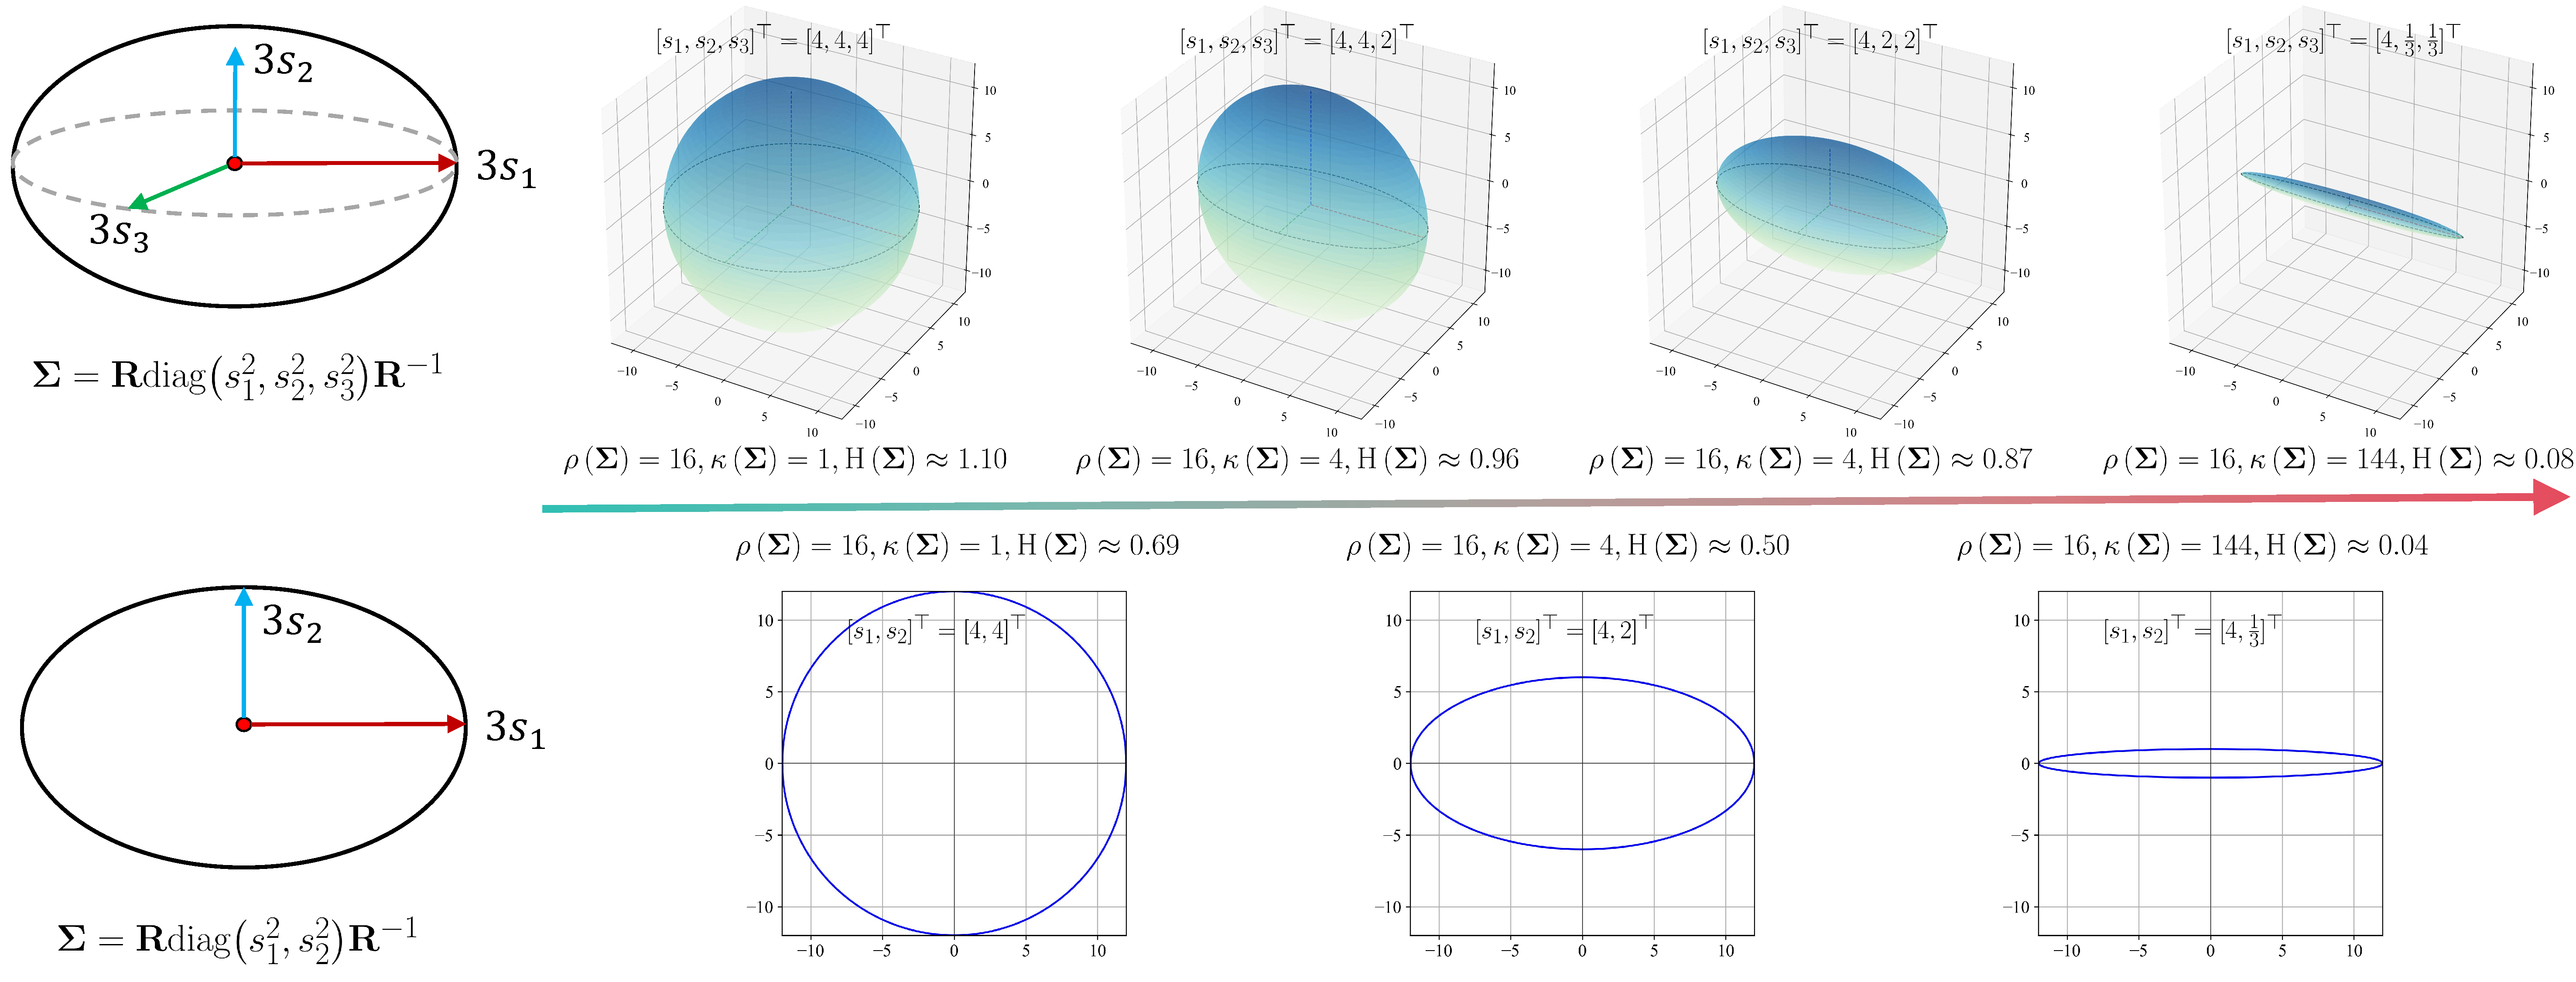
\includegraphics[width=0.85\textwidth]{figures/ch02/2409_12771_spectrum.pdf}
\caption{Huang et al.：3D 高斯基元的频谱分析：从球形高斯（等特征值）到各向异性高斯（特征值差异增大）的连续变化，针状伪影对应极端的各向异性情况。图源：Huang et al.（2024.09）~\cite{2409_12771}。}
\label{fig:02_spectrum}
\end{figure}

\paragraph{GaussianFocus}
前述有效秩和频谱分析均从高斯形状本身入手解决针状伪影，而针状伪影在感知层面的表现——边缘模糊和``空气墙''伪影——则催生了从注意力机制出发的第三条路线。GaussianFocus（2025.03）~\cite{2503_17798}修改了原始 3DGS 的训练损失环节——用注意力加权的边缘/频率约束替代均匀加权的 $L_1$ + SSIM 损失——高斯的几何参数和渲染管线保持不变。

GaussianFocus 的核心思路是：标准 3DGS 的 $L_1$ + D-SSIM 损失对所有像素区域一视同仁，无法针对边缘和高频纹理区域施加更强的优化压力。

\textbf{直觉}：想象一个老师批改作业——如果对每道题都给相同的权重，学生就可能在简单的题上花太多时间而忽略难题。GaussianFocus 引入的注意力机制就像一个``智能权重分配器''，自动找出``难题''（边缘和高频区域）并赋予更高的优化权重。为此，GaussianFocus 引入了基于补丁的注意力机制。具体而言，将渲染图像 $P_i$ 和真实图像 $G_i$ 分别切分为 $8 \times 8$ 的图像块（patch）。对每个图像块，通过 2D 卷积层分别提取查询向量 $q_{ij}$（来自渲染图像块）、键 $k_{ij}$ 和值 $v_{ij}$（来自真实图像块），注意力权重通过缩放点积计算：

\begin{equation}
w_{ij} = \mathrm{softmax}\!\bigl(q_{ij} \cdot k_{ij}^T\bigr), \quad a_{ij} = v_{ij} \cdot w_{ij},
\label{eq:02_gf_attention}
\end{equation}

其中 $a_{ij}$ 是第 $j$ 个图像块的注意力图。将所有图像块的注意力图拼接得到全局注意力图 $A_i = \sum_j a_{ij}$，再与渲染图像逐元素相乘得到注意力增强图像 $P_i' = P_i \odot A_i$。注意力机制的动机在于：真实图像的边缘和高频区域在卷积特征中具有更强的响应，注意力图自动为这些区域分配更高权重，从而在后续损失计算中加大对这些区域的优化力度。

在注意力增强图像的基础上，GaussianFocus 引入了两项互补的损失函数。边缘损失（edge loss）使用 Sobel 算子提取图像在 $x$ 和 $y$ 方向的梯度，然后计算梯度之间的 $L_1$ 距离：

\begin{equation}
\mathcal{L}_{\mathrm{Edge}} = \frac{1}{2}\bigl(\|S_x(p_i) - S_x(\hat{p}_i)\|_1 + \|S_y(p_i) - S_y(\hat{p}_i)\|_1\bigr),
\label{eq:02_gf_edge}
\end{equation}

其中 $S_x, S_y$ 是 Sobel 梯度算子，$p_i$ 和 $\hat{p}_i$ 分别是真实图像和渲染/注意力增强图像的像素值。频率损失（frequency loss）的结构与边缘损失类似，但关注的是像素值沿水平/垂直方向的变化量 $G_x, G_y$：

\begin{equation}
\mathcal{L}_{\mathrm{Frequency}} = \frac{1}{2}\bigl(\|G_x(p_i) - G_x(\hat{p}_i)\|_1 + \|G_y(p_i) - G_y(\hat{p}_i)\|_1\bigr).
\label{eq:02_gf_freq}
\end{equation}

边缘损失和频率损失的区别在于：前者通过 Sobel 算子强调边界定位的精确性，后者通过直接比较像素变化量保留高频纹理的丰富度。两者的配合使得训练同时关注``边缘在哪里''和``纹理有多细''两个层面。完整的损失函数为
\begin{equation}
\mathcal{L}_{\mathrm{Total}} = (1-\lambda_1)\mathcal{L}_1(p_i, \hat{p}_i) + \lambda_1\mathcal{L}_{\mathrm{D\text{-}SSIM}}(p_i, \hat{p}_i) + \lambda_2\mathcal{L}_{\mathrm{Edge}}(p_i, \hat{p}_i) + \lambda_3\mathcal{L}_{\mathrm{Frequency}}(p_i, \hat{p}_i),
\label{eq:02_gf_total}
\end{equation}

其中前 50 次迭代中 $\hat{p}_i$ 取注意力增强图像的像素值（即 $P_i'$ 的像素），此后切换回原始渲染图像 $P_i$ 的像素。这一设计的动机是训练初期高斯基元尚未收敛，注意力增强的梯度信号能更准确地定位需要加强优化的区域；待训练稳定后切换回原始像素以避免注意力机制的偏差累积。

此外，GaussianFocus 还引入了高斯约束策略来减少冗余基元和``空气墙''伪影。该策略包含两个组成部分。第一部分是尺度约束：对缩放矩阵中的每个尺度 $S_i$，当 $S_i > \gamma$ 时施加约束 $S_i = \gamma^{\alpha} \cdot S_i$（实验中 $\gamma = 0.3$, $\alpha = 0.2$），根据初始点云密度自适应调整——密集点云使用更低的初始尺度以减少重叠，稀疏点云使用更高的初始尺度以确保覆盖。第二部分是老化高斯的分裂过滤：对训练中存在时间较长的``老化''高斯，当其尺度 $S_{\mathrm{old}}$ 超过阈值 $\beta = 0.3$ 时选择性分裂并缩减尺度，避免不必要的冗余分裂。

如果说有效秩正则化约束了高斯的整体形状、Spectral-GS 优化了频谱特性，那么 GaussianFocus 则从感知质量的角度补充了对边缘细节的显式关注——不是修改高斯本身的形状或滤波，而是通过注意力加权和显式梯度约束来引导优化过程更加关注视觉上重要的区域。

\subsubsection{拓扑结构完整性}

针状伪影和边界模糊都源于高斯形状的局部退化，而另一类几何退化则与全局拓扑结构有关——即使单个高斯形状良好，整体的拓扑覆盖仍可能存在缺陷。标准 3DGS 从稀疏 SfM 点云初始化，低曲率区域（如白墙、平滑地面）的特征匹配稀少，导致点云覆盖不完整；而自适应密度控制（ADC）在高稀疏区域会引起大幅高斯位移，其他点云增强方法（如致密化、分裂）同样存在破坏拓扑结构的风险。

\paragraph{Topology-GS}
Topology-GS（2024.12）~\cite{2412_16619}修改了原始 3DGS 的初始化和训练监督环节——用拓扑感知插值替代直接点云初始化、用拓扑正则化损失补充标准 $L_1$ + SSIM 损失——高斯的渲染管线和密度控制保持不变。

\textbf{术语铺垫}：持久同调（Persistent Homology）是拓扑数据分析的核心工具。直觉上，它可以检测点云中的``洞''和``连通分量''——把点云想象成不断膨胀的气球，膨胀过程中某些洞被填满、某些新的连通分量合并，``持久''指的是那些在整个膨胀过程中存活最久的拓扑特征，它们对应场景中最重要的结构（如墙面的连续性、物体的连通性）。Topology-GS 首次将这一工具引入 3DGS 优化，从全局拓扑而非局部形状的角度解决覆盖不完整问题。该方法包含两个核心组件：局部持久 Voronoi 插值（LPVI）解决初始化稀疏问题，拓扑正则化损失（PersLoss）在训练中约束渲染结果的拓扑特征完整性。

\paragraph{局部持久 Voronoi 插值（LPVI）。}LPVI 的设计动机是：在低曲率区域直接进行 3D 插值容易引入拓扑噪声（如在平面表面附近生成孤立点簇），但在局部切平面上做 2D 插值则安全得多——因为流形学习假设高维数据位于低维流形上，而非孤立点的切空间近似为切平面。LPVI 的核心机制是在 3D 和 2D Voronoi 插值之间自适应切换，切换依据是插值前后的拓扑变化程度。

\textbf{直觉}：就像在一张稀疏的点阵图上填空——如果填完后``洞''的数量和位置没有明显变化，说明填空是安全的；如果突然出现了不该有的``洞''，就说明填法有问题，需要换一种更保守的方式。具体地，对稀疏点云 $X = \{x_1, \ldots, x_m\} \subset \mathbb{R}^3$ 中的每个点 $x_l$，LPVI 首先找到其 $K$ 近邻，执行 3D Voronoi 剖分得到候选插值点集 $\{v_1, \ldots, v_p\}$。然后计算拓扑变化评估函数：

\begin{equation}
\mathrm{TopoDiff}(X_l, \tilde{X}_l) = W_{\mathrm{Dist}}\!\bigl(\mathrm{PD}(X_l),\;\mathrm{PD}(\tilde{X}_l)\bigr),
\label{eq:02_topodiff}
\end{equation}

其中 $X_l = \{x_l, x_{\iota_1}, \ldots, x_{\iota_K}\}$ 是以 $x_l$ 为中心的近邻集，$\tilde{X}_l = X_l \cup \{v_1, \ldots, v_p\}$ 是加入插值点后的扩展集，$W_{\mathrm{Dist}}$ 是持久图（Persistence Diagram）之间的 Wasserstein 距离。若拓扑变化低于阈值 $\tau$（即 $\mathrm{TopoDiff} < \tau$），说明 3D 插值未破坏局部拓扑结构，直接接受所有候选点；若超过阈值，则切换至 2D 模式——对 $K'$ 个近邻做 PCA 降维至切平面，在该平面上执行 2D Voronoi 剖分，再将顶点通过主成分向量 $U = [u_1, u_2]$ 映射回 3D 空间。这一降维策略利用了平面表面数据的内在低维结构，既避免了拓扑破坏，又在低曲率区域实现了有效的点覆盖增强。

\paragraph{拓扑正则化损失（PersLoss）。}LPVI 解决了初始化稀疏问题，但训练过程中仍缺乏对拓扑特征的约束——标准 3DGS 的 $L_1$ + SSIM 损失仅约束像素级颜色相似性，无法保证特征级的结构完整性（如局部纹理模式和全局语义关系），导致高 LPIPS 值。PersLoss 的设计思路是：将渲染图像和真实图像从 2D 像素空间重新解读为 3D RGB 空间中的点云（$y' = S(y), \hat{y}' = S(\hat{y})$，其中 $S$ 将 $H \times W \times 3$ 图像重塑为 $HW \times 3$ 矩阵），然后在该空间中计算持久同调。具体地，使用 alpha 复形对两个 RGB 点云进行过滤，得到各维同调的持久条形码（Persistent Barcode），其中每条 bar 的长度 $(b^k, d^k)$ 表示一个拓扑特征的生存范围——越长的 bar 对应越重要的拓扑特征。为过滤噪声，只保留每个维度的前 $k_i$ 个最长条（$i = 0, 1, 2$ 分别对应 0 维、1 维、2 维同调），得到截断持久条形码 $pb$ 和 $\hat{pb}$。PersLoss 定义为两者之间出生-死亡值的总差异：

\begin{equation}
\mathcal{L}_{\mathrm{Pers}} = \sum_{i=0}^{2}\;\frac{1}{\beta^i \sum_{k=0}^{2} k^k}\;\sum_{j=1}^{k_i}\Bigl(\bigl|b^i_j - \hat{b}^i_j\bigr|^2 + \bigl|d^i_j - \hat{d}^i_j\bigr|^2\Bigr),
\label{eq:02_persloss}
\end{equation}

其中 $\beta^i$ 是第 $i$ 维 Betti 数，归一化项 $\sum_{k=0}^{2} k^k$ 用于平衡各维度的贡献。最终拓扑感知总损失为 $\mathcal{L}_{\mathrm{total}} = \mathcal{L}_{\mathrm{supv}} + \lambda_{\mathrm{topo}} \mathcal{L}_{\mathrm{Pers}}$，其中 $\mathcal{L}_{\mathrm{supv}}$ 是标准的 $L_1$ + SSIM 监督损失。Topology-GS 理论证明了在温和正则性假设下，该拓扑感知损失在有限迭代次数内收敛（步长选取 $O(1/\epsilon)$），确保了与 ADC 机制配合的实用性。

Topology-GS 与前述形状正则化方法形成互补：形状正则化确保每个高斯基元的局部质量，拓扑分析则确保基元群体的全局覆盖完整性——前者约束“每个高斯是否形状正确”，后者约束“高斯集合是否完整覆盖了场景的拓扑结构”。

\subsection{浮游体与虚假透明度}

前述边界与几何退化伪影源于高斯形状的局部缺陷，而浮游体和虚假透明度则源于 $\alpha$-混合 优化本身的欠约束性。即使高斯形状正确，不透明度优化仍可能收敛到错误的局部极小值。

\subsubsection{浮游体伪影的成因与消除}

浮游体（floater）是 3DGS 重建中最顽固的伪影之一，表现为脱离实际几何的半透明高斯簇。StableGS（2025.03）~\cite{2503_18458}修改了原始 3DGS 的不透明度参数化环节——用双不透明度架构替代单一不透明度——高斯的颜色、位置、协方差参数保持不变。StableGS 首次揭示了浮游体的根本成因，并提出双不透明度架构系统性地解决这一问题。

\paragraph{伪均衡与梯度消失。}\textbf{直觉}：浮游体的颜色误差就像一群人投票——有的投正票、有的投负票，恰好互相抵消，看起来``总分为零''，但实际上每个人的票都是错的。StableGS 考虑一个简化场景：聚焦于一个浮游体簇，有 $M$ 条光线穿过它，对应的真实颜色为 $\{c_m^{gt}\}_{m=1}^M$。假设场景其余部分已被完美重建（穿过簇后的背景色等于真实颜色），则理论最优解是所有浮游体不透明度 $\alpha_k = 0$。然而优化经常陷入非全局极小值：浮游体簇的累积颜色 $c_f = \sum_{k=1}^{K_f} c_k \alpha_k(x_k^{r_m}) \bar{T}_k$ 达到``伪均衡''状态——跨视角颜色误差的符号几乎相互抵消：

\begin{equation}
\sum_{m=1}^{M}\bigl(c_f - c_m^{gt}\bigr) \approx 0.
\label{eq:02_pseudo_equilibrium}
\end{equation}

对于 $L_1$ 损失，这一条件直接导致 $c_f$ 的梯度趋近于零，由链式法则引起不透明度 $\alpha_k$ 和颜色 $c_k$ 参数梯度的级联消失。实验验证了这一现象在 $L_1$、MSE 甚至交叉熵损失下普遍存在——梯度消失使优化器无法有效降低浮游体不透明度，模型被困在几何错误但光度损失极低的局部极小值。然而，浮游体在几何维度（深度）上的误差是显著且无歧义的，这启发了引入基于深度的损失来提供独立、更强的几何监督信号。

\paragraph{双不透明度架构：几何与外观的防火墙。}直接在标准 3DGS 上引入深度损失虽可消除浮游体，但会损害渲染细节——深度损失的强梯度来自不可避免地含噪声和不准确的外部先验，会污染所有高斯参数，导致纹理模糊；对半透明物体（如玻璃、水面）则更严重地破坏渲染精度。为此，StableGS 为每个高斯 $G_k$ 引入额外的可学习辅助不透明度参数 $\alpha'_k \in [0,1]$，定义两种不透明度函数：

\begin{equation}
\underbrace{\alpha_k(x)}_{\text{几何不透明度}} = \alpha_k \exp\!\bigl(-\tfrac{1}{2}(x-\mu_k)^T\Sigma_k^{-1}(x-\mu_k)\bigr), \qquad
\underbrace{\alpha'_k(x)}_{\text{渲染不透明度}} = \alpha'_k \cdot \alpha_k(x).
\label{eq:02_dual_opacity}
\end{equation}

几何不透明度仅依赖原始参数 $\alpha_k$，渲染不透明度则由两个参数联合决定。对应两条功能解耦的渲染路径：
\begin{itemize}
    \item \textbf{几何正则化路径}：用几何不透明度 $\alpha_k(x)$ 渲染中间颜色图 $C^s$ 和深度图 $D^s$，输出专用于深度损失监督——强几何约束的梯度直接作用于基础参数 $\alpha_k$，有效消除浮游体，但细节损失被隔离在此路径内；
    \item \textbf{外观精炼路径}：用渲染不透明度 $\alpha'_k(x)$ 渲染最终颜色图 $C^o$ 和深度图 $D^o$——凭借可学习的 $\alpha'_k$，此路径屏蔽了几何路径中的粗糙梯度，在稳定的几何支架之上专注于学习精细颜色和半透明效果。
\end{itemize}
这一解耦设计是深度损失真正有效的关键：可以在几何路径上放心施加强约束，而外观路径保持自由表达能力。

\paragraph{双路径损失函数。}总损失由颜色损失和几何损失组成：$\mathcal{L}_{\mathrm{total}} = \mathcal{L}_{\mathrm{color}} + \lambda_g \mathcal{L}_{\mathrm{geometry}}$。颜色损失监督两条路径：

\begin{equation}
\mathcal{L}_{\mathrm{color}} = \mathcal{L}_{\mathrm{3DGS}}(C^o, C^{gt}) + \lambda_s \mathcal{L}_1(C^s, C^{gt}),
\label{eq:02_stable_color}
\end{equation}

其中第一项对最终渲染输出施加标准 $L_1$ + D-SSIM 损失，第二项以 $\lambda_s$ 加权鼓励几何路径尽可能解释场景的不透明部分。因此辅助参数 $\alpha'_k$ 的梯度主要来自几何路径无法完美建模的区域（如半透明表面和精细结构），实现了几何与外观的自动分工。几何损失 $\mathcal{L}_{\mathrm{geometry}}$ 包含两项互补的正则化：自监督深度一致性损失利用场景固有的多视角一致性纠正几何错误，基于单目深度估计的外部几何先验则专门处理弱纹理区域。

\paragraph{自监督深度一致性损失。}核心思想是：从视角 $i$ 渲染的深度图 $D_i^s$ 经可微分变换投影到视角 $j$ 后，应与直接从视角 $j$ 渲染的深度图 $D_j^s$ 一致。浮游体的深度值通常是自身深度与背景深度的平均值，经变换后产生大的不一致性，提供强梯度信号。对选定的图像对集合 $\mathcal{P}$：

\begin{equation}
\mathcal{L}_{\mathrm{consis}} = \sum_{(i,j) \in \mathcal{P}} \bigl(\|W_{i \to j}(D_i^s) - D_j^s\|_1 + \|W_{j \to i}(D_j^s) - D_i^s\|_1\bigr),
\label{eq:02_depth_consis}
\end{equation}

其中 $W_{i \to j}$ 是利用已知相机姿态的可微分变换算子。为保证损失稳定性，训练对的选取需满足三个条件：两视角共可见特征点 $>30$（确保足够重叠）、相对旋转角 $16^\circ\text{--}60^\circ$（防止极端基线）、符合单应性矩阵的特征点比例 $< 0.8$（抑制纯旋转退化）。

\paragraph{外部几何先验与全局尺度优化。}弱纹理区域（白墙、平滑地面）缺乏视觉特征，自监督约束不足以提供有效几何信号。StableGS 引入单目深度估计模型 DUSt3R 的先验：对图像对 $(i,j)$，DUSt3R 输出各自相机坐标系下的 3D 点图及置信度图。关键瓶颈在于每对预测存在于独立的未知尺度下，无法直接用于全局 3D 重建。StableGS 提出高效全局尺度优化算法，将原本高维的点云对齐问题通过矩阵分解等价变换压缩为仅 7 个``等价点''上的低维优化，高效求解所有图像对的全局一致尺度因子 $S = \{s_{i,j}, s_{j,i}\}_{(i,j) \in \mathcal{P}}$。最终几何先验损失为
\begin{equation}
\mathcal{L}_{\mathrm{prior}} = \sum_{(i,j) \in \mathcal{P}} \bigl(D(i,j) + D(j,i)\bigr), \quad D(i,j) = \frac{1}{\|d_{i,j}\|_0} \sum C^{1,1}_{i,j} \bigl|D_i^s - d_{i,j}\bigr|,
\label{eq:02_geom_prior}
\end{equation}

其中 $d_{i,j} = s_{i,j} X^{1,1}_{i,j}[z]$ 是尺度校正后的深度图，$C^{1,1}_{i,j}$ 是置信度图。总几何损失为 $\mathcal{L}_{\mathrm{geometry}} = \lambda_c \mathcal{L}_{\mathrm{consis}} + \lambda_p \mathcal{L}_{\mathrm{prior}}$。StableGS 的完整框架在多个基准上实现了 SOTA 几何精度和视觉质量。

StableGS 从优化动力学的视角解释了浮游体为何在标准训练中无法被消除——不透明度梯度因伪均衡而消失。EFA-GS（2025.08）~\cite{2508_02493}则从频域角度提供了互补的分析：与 StableGS 在不透明度参数化上做文章不同，EFA-GS 修改了密度控制环节——用基于累积梯度的选择性扩展替代标准 ADC 的统一分裂——高斯的其他参数保持不变。EFA-GS 关注的是浮游体在训练早期如何产生。

\paragraph{频域视角：欠优化高斯的产生机制。}EFA-GS 的分析起点是采样定理在高斯泼洒中的对应：每个高斯的尺度决定其能接收的频率信息，坐标决定其对应的采样率。当高斯尺度大于 Nyquist 采样间隔时，该高斯可以从训练视角获得充分优化（过优化高斯）；反之，尺度小于采样间隔的高斯则处于欠优化状态——它们接收的光线更少、投影到更少的像素上，梯度天然偏小。EFA-GS 发现，低质量初始化（如 SfM 点云稀疏或含噪）会迫使高斯在训练早期急剧收缩——尺度在仅约 5000 次迭代内就快速坍缩——噪声进一步放大这一效应，使大量高斯在尚未学到准确低频信息之前就已缩至 Nyquist 间隔以下，成为欠优化高斯。这些欠优化高斯虽然对训练视角的渲染影响有限（过优化高斯可以通过训练修正其误差），但对测试视角却造成严重退化——因为测试视角从未参与训练，欠优化高斯无法被修正，最终表现为脱离几何的浮游伪影。

\paragraph{Mip-splatting 的低通滤波为何失效。}直觉上，低通滤波应能帮助小高斯优先学习低频信息。Mip-splatting 确实采用了低通滤波策略，但 EFA-GS 指出其两个根本局限：（1）高斯尺度的坍缩速度极快且非平稳，静态低通滤波器无法跟上这种动态变化；（2）过优化高斯和欠优化高斯应被区别对待，但 Mip-splatting 对同一深度的所有高斯施加相同的低通滤波——既未选择目标高斯，也未动态调整滤波强度。

\paragraph{LFCF 算法：基于累积梯度的选择性扩展。}基于上述分析，EFA-GS 提出 Low-Frequency-Come-First（LFCF）算法。核心思路是：较小的高斯接收更少光线，梯度天然偏小，因此梯度反常上升是异常信号。LFCF 为每个高斯维护累积梯度 $PGrad(i)$，在第 $t$ 次迭代时将其与当前梯度 $Grad(i)$ 比较：
\begin{itemize}
    \item 若 $Grad(i) > PGrad(i)$：该高斯可能是正在恶化为浮游伪影的欠优化高斯，执行扩展操作 $s_i^* = s_i \cdot c$（$c > 1$），强制其先学习低频信息再逐步优化高频细节；
    \item 若 $Grad(i) < PGrad(i)$：该高斯可能是过优化高斯，执行收缩并分裂 $s_i^* = s_i \cdot c$（$c < 1$），促进细节表达；
    \item 更新累积梯度 $PGrad(i) \leftarrow Grad(i)$。
\end{itemize}
扩展和收缩操作的统一形式为 $s^* = s \cdot c^3$，其中 $c > 1$ 对应扩展、$c < 1$ 对应收缩。

\paragraph{自适应扩展范围：深度策略与尺度策略。}然而，对所有高斯施加统一的扩展因子 $c$ 会在复杂场景中侵蚀远处细节——深度越大的高斯采样率越低、越难优化，统一扩展会过度放大其尺度。为此，EFA-GS 设计了两个互补策略：

\textbf{深度策略}：采样率越低（深度越大）的高斯，赋予越小的扩展因子。具体地，先按 Mip-splatting 的方式计算每个高斯的采样率，再将其投影到 $[0,1]$ 作为线性插值因子 $\lambda(i)$，最终扩展因子为 $c(i) = \lambda(i) \cdot c_{max} + (1 - \lambda(i)) \cdot c_{min}$，其中 $c_{min}$ 通常设为 1（即不扩展采样率最低的高斯），$c_{max}$ 设为 1.5。

\textbf{尺度策略}：高斯沿不同轴的缩放因子对应不同的采样间隔，应区别对待。为保持高斯体积不变，EFA-GS 设定约束 $\prod_i c_i = 1$，在此约束下扩展最短轴、收缩最长轴——使扩展操作不改变总体积，而是调整形状以匹配各方向的采样需求。

在自建 RWLQ 数据集上，EFA-GS 相比基线 Mip-splatting 的 PSNR 提升 1.68 dB，同时在高质量数据集 Mip-NeRF 360 上也能保持甚至略微提升性能，表明深度/尺度策略有效平衡了去伪影与保细节的矛盾。

在 StableGS 和 EFA-GS 分别从优化动力学和频域角度解决浮游体之后，后续工作将 3DGS 优化本身重新框架化。Denoising-GS（2026.05）~\cite{2605_14880}不沿用浮游体的成因分析框架，而是将整个 3DGS 优化重新定义为高斯基元去噪过程——含噪初始点云中的离群高斯即为``噪声''，通过空间感知去噪框架从含噪初始点云中恢复高质量重建。3DGS-HPC（2026.03）~\cite{2603_07587}则将浮游体问题与瞬态干扰关联起来，提出混合 Patch 级分类策略用于无干扰物的 3DGS 重建，有效区分静态场景和瞬态干扰物——这一思路将在本节后续的瞬态物体部分进一步展开。

\subsubsection{虚假透明度}

\paragraph{NGS}
浮游体是脱离几何的游离高斯，而虚假透明度则表现为本应不透明的表面被错误地重建为半透明——两者同属 $\alpha$-混合 欠约束问题，但表现不同。NGS（2025.10）~\cite{2510_15736}修改了原始 3DGS 的训练初始化环节——用内部噪声注入替代直接训练——高斯的渲染管线保持不变。NGS 首次系统识别了 3DGS 中的虚假透明度问题：不透明物体表面被错误地重建为半透明，在交互式观察中背景和内部模式随相机运动而不一致地变化。

\paragraph{透明度歧异的数学根源。}\textbf{直觉}：想象一扇半透明的玻璃窗——透过它可以看到后面的墙。问题在于，``玻璃半透明 + 墙壁清晰''和``玻璃不透明 + 墙壁不可见''在像素颜色上可以给出完全相同的结果，优化器无法区分这两种情况，因此会``偷懒''选择更容易的半透明解。NGS 的分析直接回到 $\alpha$-混合 公式。对于像素 $p$，标准 3DGS 的渲染结果为 $C(p) = \sum_i \alpha_i c_i \prod_{j<i}(1-\alpha_j)$，训练目标为复合 $L_1$ + SSIM 光度损失 $L_{photo}$。问题出在分解方式：令 $s$ 为沿光线遇到的第一个表面高斯的索引，$B$ 为其后方所有高斯的集合，则渲染颜色可分解为
\begin{equation*}
C(p) = \underbrace{\alpha_s c_s}_{\text{前表面}} + (1-\alpha_s) \underbrace{\sum_{i \in B} \alpha_i c_i \prod_{s<j<i}(1-\alpha_j)}_{\text{背景（当 $\alpha_s < 1$ 时泄漏）}}
\end{equation*}

对于任意半透明表面（$\alpha_s < 1$），总存在一组背景不透明度和颜色能复现完全相同的像素颜色——即与完全不透明表面给出相同的光度损失。梯度下降因此可以接受 $\alpha_s$ 偏低的平凡最小值。这一问题在 360 度物体扫描中尤为严重：前后表面沿同一光线配对，深度间距小，两者被联合优化，虚假透明度更易发生。

\paragraph{NGS 的解决方案：内部噪声注入。}在解决方案层面，NGS 与前述 StableGS 的策略形成鲜明对比：StableGS 通过双不透明度架构分离几何与外观路径，本质上是在渲染管线中增加一条辅助路径；NGS 则不需要修改渲染管线，而是通过在物体体积内部注入不透明噪声高斯来填充表面后方空间，从物理上阻断前后表面之间的视线通道，迫使表面高斯提高不透明度。其流程分为四个阶段：

\textbf{初始化}：从现有高斯的均值计算凸包网格（Quickhull），将凸包体素化为粗占据网格，在每个占据体素内生成一个随机颜色的噪声高斯点。

\textbf{深度剪枝}：凸包包含物体外部区域，因此需对每个视角的每个像素，利用 3DGS 的深度排序移除出现在表面高斯前方的噪声高斯，再腐蚀占据网格以确保噪声高斯与表面之间保持缓冲距离。

\textbf{多尺度注入}：以从粗到细的方式在多个体素分辨率上重复初始化与剪枝——仅在不包含上一级噪声高斯的体素中生成新噪声——在保持低内存开销的同时覆盖精细几何。

\textbf{微调与引导训练}：冻结表面高斯，仅训练噪声高斯的不透明度并剪枝错误放置的噪声；此后冻结噪声高斯，解冻表面高斯并重置学习率，让表面参数在新优化空间中正常训练。关键设计：每次迭代随机设置噪声高斯的颜色（从六种高对比度原色/次级色中选取），防止噪声不透明度过拟合到表面颜色——确保优化仅基于遮挡效果而非颜色匹配。

\paragraph{透射率评估指标 SOS。}标准质量指标（PSNR、SSIM、LPIPS）基于静态图像对比较，无法量化视角不一致性——虚假透明度下的渲染仍可报告高分。NGS 利用噪声高斯点云设计了诊断工具：将噪声高斯和表面高斯分别着为纯色（如绿色和红色），用标准光栅化器渲染后，噪声颜色通道即为表面透射率图 $T_i$。定义透射率评分：

\begin{equation*}
SOS_i = \left(\frac{\sum T_i / |M_i| + \epsilon}{\log(10)}\right)
\end{equation*}

其中 $M_i$ 为前景分割掩码，$\epsilon = 10^{-10}$ 保证数值稳定性。$SOS_i = 1$ 表示完全不透明表面，$SOS_i \approx 0$ 表示完全透明表面。这一指标无需交互式观察即可在静态渲染中量化虚假透明度。NGS 还发布了噪声注入插件数据集（包括 DTU 的注入版本和高分辨率物体扫描数据集），为这一此前被忽视的伪影类型建立了评估基准。

\subsection{瞬态物体与动态干扰}

前述浮游体和虚假透明度源自 3DGS 内部的优化缺陷，而另一类伪影则由外部因素引起——真实世界场景中普遍存在的瞬态物体（行人、车辆、阴影变化等）破坏了 3DGS 所需的多视角一致性假设。忽略这些干扰物会导致模糊效果和浮游体伪影。

\subsubsection{瞬态干扰处理方法}

T-3DGS（2024.12）~\cite{2412_00155}修改了原始 3DGS 的训练数据选取环节——用无监督瞬态掩码替代全像素训练——高斯的渲染管线和参数化保持不变。T-3DGS 提出无监督瞬态检测与双向追踪框架，为瞬态物体处理建立了重要基线。相对于标准 3DGS 对所有像素不加区分地进行训练，T-3DGS 的核心创新在于其重建不确定性预测器（RUP）利用 3DGS 重建过程本身的训练动态来识别瞬态区域——通过散度度量区分静态和动态元素，完全无需显式监督。瞬态掩码细化器利用 SAM2 进行双向时空掩码传播，增强检测的边界精度和时序一致性。该方法还能处理半瞬态物体（同一物体在视频中有静态和动态两种状态），在稀疏和密集视频数据集上显著优于 WildGaussians、SpotlessSplats 等方法。

\paragraph{RobustSplat}
T-3DGS 聚焦于检测已存在的瞬态伪影——即在训练完成后识别并隔离瞬态区域，但此时瞬态物体可能已经对静态场景的重建造成了不可逆的干扰。RobustSplat（2025.06）~\cite{2506_02751}则从预防角度出发，发现了瞬态物体渗入重建的更早入口：高斯致密化过程（分裂/克隆操作）在早期优化阶段就会无意中拟合瞬态物体，因为梯度累积超过阈值时无论静态还是动态区域都会触发致密化。与 T-3DGS 的无监督检测不同，RobustSplat 提出延迟高斯增长策略，优先优化静态场景结构后再允许致密化，同时设计尺度级联掩码引导方法：先利用低分辨率特征相似性（语义一致性更强）获取可靠初始掩码，再逐步过渡到高分辨率实现精确掩码预测。简言之，T-3DGS 是``先训练再检测''，RobustSplat 是``先过滤再训练''——两者分别覆盖了瞬态物体处理的事后和事前两个阶段。

\subsection{渲染一致性与感知增强}

前面的讨论聚焦于特定类型伪影的消除，本节转向更一般的渲染一致性问题——即使没有明显的伪影，训练视角的有限性、遮挡关系和光学畸变也会导致新视角渲染质量下降。

\subsubsection{视角一致性}

\paragraph{PEP-GS}
训练视角的有限性导致新视角渲染质量显著下降。PEP-GS（2024.11）~\cite{2411_05731}针对标准球谐函数（SH）在复杂光照下难以捕获各向异性颜色分量的问题，提出用层次粒度结构注意力机制替代传统 SH 颜色表示，通过多粒度注意力捕获局部几何特征和复杂视角相关颜色变化。同时引入 Kolmogorov-Arnold 网络进行不透明度和协方差估计，以及归一化拉普拉斯金字塔距离（LapL1）感知损失增强跨视图感知一致性。

\paragraph{极端视角过滤与物理约束增强}
PEP-GS 通过增强颜色表示提升一般视角的渲染质量，而极端视角下的渲染退化则需要更激进的策略。Extremely Views（2025.10）~\cite{2510_20027}不走表示增强路线，而是提出实时渲染感知过滤方法，在旋转对齐坐标系中评估各向异性高斯的不稳定性，通过基于中间梯度的敏感度评分和两遍过滤策略直接移除不稳定基元。与 Extremely Views 直接移除不稳定基元的``做减法''策略不同，Depth-Consistent 3DGS（2025.11）~\cite{2511_10316}从物理约束角度``做加法''增强一致性，结合景深监督（散焦卷积和景深损失）与多视角一致性监督（LoFTR 特征匹配和最小二乘优化），从物理散焦建模和几何约束两个角度增强渲染一致性。三者形成递进：PEP-GS 改进颜色表示以应对一般视角退化，Extremely Views 过滤不稳定基元以应对极端视角，Depth-Consistent 3DGS 引入物理约束从根源上增强多视角一致性。

\subsubsection{可渲染性与感知修复}

视角一致性问题在均匀观测条件下尚可控制，但非均匀观测（训练视角分布不均）和严重遮挡场景下的渲染不一致更具挑战。

\paragraph{RF-GS}
RF-GS（2025.04）~\cite{2504_19261}针对非均匀观测场景的渲染不稳定问题，提出可渲染场（renderability field）量化输入不均匀性，引导伪视图采样增强视角覆盖，并训练图像恢复模型将点投影图映射为可见光风格图像。

\paragraph{Proxy-GS}
RF-GS 通过补充虚拟视角缓解覆盖不足，但非均匀观测的另一个后果——遮挡区域的不一致性——需要不同的策略。Proxy-GS（2025.09）~\cite{2509_24421}正是从遮挡感知角度切入同一问题。与 RF-GS 生成新视角不同，Proxy-GS 利用轻量代理网格实现遮挡感知，能在 $1000 \times 1000$ 分辨率下 1ms 内生成精确遮挡深度图。代理系统同时引导锚点和高斯的剔除以加速渲染，以及训练中的致密化趋向表面避免遮挡区域的不一致性，在 MatrixCity Streets 等重遮挡场景上实现 2.5 倍以上加速。

\paragraph{ArtiFixer：后处理修复}
前述方法均在优化阶段解决一致性问题，但即使经过精心优化，渲染结果中仍可能残留伪影和缺失区域。ArtiFixer（2026.03）~\cite{2603_00492}将修复时机推至后处理阶段，利用双向自回归扩散模型增强和扩展 3D 重建，通过生成模型修复渲染伪影和缺失区域，实现从部分观测到完整场景的扩展重建。ArtiFixer 与 RF-GS 和 Proxy-GS 形成互补：RF-GS 在训练阶段补充视角覆盖，Proxy-GS 在优化阶段处理遮挡，ArtiFixer 在后处理阶段修复残余缺陷——三者覆盖了渲染一致性保障的完整流程。

\subsubsection{光学像差场景}

\paragraph{DGS}
前述一致性问题均假设成像系统本身是标准的，但 XR 设备和野外机器人常采用保护盖覆盖前向摄像头，盖体表面不规则性导致光学像差（模糊和非参数畸变），使标准 3DGS 无法正常工作。SynthCover（2024.11）~\cite{2411_06365}针对这一特殊场景，提出折射场（Refractive Field）估计保护盖几何，通过精确的解析计算折射光线实现透过保护盖的新视角合成，并与场景表示联合优化以捕捉非对称的表面不规则性。

\begin{takeaway}
3DGS 的系统性伪影（针状伪影、浮游体、虚假透明度）各有不同成因——从高斯连续性本质到 ADC 的形状退化。解决方案涵盖正则化、瞬态物体处理、感知增强和后处理修复，RF-GS、Proxy-GS 和 ArtiFixer 三者覆盖了从训练到后处理的渲染一致性保障完整流程。
\end{takeaway}

%% ============================================================
\section{多模态与跨域渲染}
\label{sec:02_10}

3D Gaussian Splatting 的标准渲染管线本质上是为 RGB 图像驱动的场景表示设计的——高斯基元的颜色由球谐函数（SH）参数化，训练损失基于渲染图像与输入 RGB 图像的光度差异。这一设计假设输入数据为常规视角下捕获的标准彩色图像，然而现实世界的感知模态远不止于此。深度传感器提供几何信息、热红外相机捕获温度分布、事件相机输出异步亮度变化、脉冲相机产生高时间分辨率二值流、LiDAR（Light Detection and Ranging，激光雷达）生成精确三维点云、射频信号携带电磁波传播信息。这些非 RGB 模态的物理特性与标准光学成像存在根本差异，无法直接嵌入 3DGS 的训练框架。各方法如何扩展 3DGS 的表示和渲染机制以适配不同模态的物理约束，是本节的核心议题。表~\ref{tab:02_modalities} 汇总了本节涉及的七种非 RGB 模态及其核心挑战。

\begin{table}[htbp]
\centering
\small
\caption{多模态 3DGS 渲染应用汇总}
\label{tab:02_modalities}
{\hbadness=10000
\begin{tabular}{l l p{5.8cm}@{\hspace{0.5em}}}
\toprule
\textbf{模态} & \textbf{核心挑战} & \textbf{代表方法} \\
\midrule
事件相机 & 异步稀疏事件流，无纹理监督 & Ev-GS~\cite{2407_11343}, Elite-EvGS~\cite{2409_13392} \\
脉冲相机 & 40KHz 二值脉冲，时序积分 & SpikeGS~\cite{2407_03771} \\
水下 & 散射+吸收，介质建模 & WaterSplatting~\cite{2408_08206}, SeaSplat~\cite{2409_17345} \\
LiDAR & 精确 3D 点云，细节缺失 & LiDAR-3DGS~\cite{2409_16296} \\
热红外 & 温度分布，视角依赖 & Veta-GS~\cite{2505_19138}, TDg~\cite{2605_30328} \\
音频 & 衍射+散射，模态密度差异 & AV-GS~\cite{2406_08920} \\
射频 & 电磁波传播，跨域物理 & RF-3DGS~\cite{2411_19420}, WRF-GS~\cite{2412_04832} \\
\bottomrule
\end{tabular}
}
\end{table}

\subsection{神经形态视觉：事件相机与脉冲相机}

本节介绍两类神经形态传感器在 3DGS 中的应用：事件相机（事件信号替代 RGB 监督、Ev-GS 等）和脉冲相机（脉冲-渲染关联）。

\subsubsection{事件相机}

事件相机以微秒级时间分辨率异步捕获像素级亮度变化，输出稀疏的事件流而非固定帧率的图像。其高动态范围（$>$120 dB）和极低延迟使其在高速运动和低光照场景中具有天然优势，但事件流的稀疏性和缺乏纹理信息给 3DGS 训练带来两个根本性挑战。一是无法直接构建光度损失（事件只记录变化量而非绝对亮度），二是缺乏纹理信息导致 3DGS 的 SfM 初始化流程失效。

\paragraph{事件信号替代 RGB 监督。} Ev-GS（2024.07）~\cite{2407_11343}修改了原始 3DGS 的训练监督环节——用时间窗口内的事件累积信号替代逐像素 RGB 光度损失——高斯基元的几何与渲染表示保持不变。标准 3DGS 的训练损失要求渲染图像与输入 RGB 图像之间的光度差异，但事件相机不输出绝对亮度。Ev-GS 的核心洞见是：事件信号本质上编码了亮度变化的梯度信息。具体而言，在两个时间戳 $t_1, t_2$ 分别用 3DGS 渲染图像 $I(t_1)$ 和 $I(t_2)$，利用亮度差 $\Delta L = \log I(t_2) - \log I(t_1)$ 与对应时间窗口内累积事件帧 $E$ 的理想关系 $E = \Delta L / \Delta$（$\Delta$ 为对比度阈值）构建可微分损失 $L = \|\Delta L / \Delta - E\|^2$。这意味着 Ev-GS 将标准 3DGS 逐像素的光度监督替换为时间窗口内的事件累积监督。该方法不需要任何 RGB 或灰度帧数据，完全在事件域内完成训练。在运动模糊场景中，该方法 PSNR 比基于帧的方法高 2--4 dB，因为事件相机本身不受运动模糊影响，Ev-GS 恰好利用了这一物理优势。

\paragraph{Ev-GS 实现细节。} 上述事件监督框架的设计背后有三个关键工程决策。

\textbf{初始化策略。} 标准 3DGS 使用 COLMAP SfM 流程从多视角图像中恢复初始点云和相机位姿，但事件流是异步稀疏的亮度变化信号，不包含纹理和绝对亮度信息，SfM 无法直接运行。Ev-GS 因此采用随机初始化策略：在场景包围盒内均匀采样 $10^6$ 个点作为初始 3D 高斯集合。这一策略之所以可行，是因为 Ev-GS 的损失函数仅约束渲染结果的\emph{变化量}而非绝对亮度——即使初始点云的位置和颜色完全随机，事件监督信号仍然能够驱动高斯向正确位置收敛。代价是收敛速度慢于 SfM 初始化的方案，后续工作 Elite-EvGS 正是从这一问题切入加以改进。相机位姿则来自外部传感器标定：合成数据直接使用已知渲染轨迹，真实数据通过将物体置于匀速转台、相机保持静止的方式精确控制。

\textbf{时间窗口与对数亮度转换。} Ev-GS 设定最大事件窗口长度 $W = 50$ 帧，每次训练迭代从中随机选取 $w \in [1, W]$ 作为实际窗口。随机选取窗口长度的设计动机是：短窗口对应微小亮度变化，提供精细的局部梯度信息；长窗口对应较大亮度变化，提供全局结构约束。随机采样使模型同时暴露于两种尺度的监督信号。渲染结果从线性空间转换到对数亮度空间的过程为 $L(I_t) = \log((I_t)^g + \epsilon)$，其中 $\epsilon = 10^{-5}$ 防止零值取对数，$g = 4.8$ 是灰度 gamma 校正值（BT.601 标准推荐的平滑近似）。这一 gamma 校正之所以必要，是因为事件相机的对比度阈值 $\Delta$ 定义在传感器原始输出的对数域中，而 3DGS 渲染的灰度值在线性域，gamma 校正弥合了两个域之间的非线性差异。

\textbf{Linlog 映射与损失函数。} 直接在对数域计算 $L_2$ 损失在低亮度区域（接近零的值）会产生数值不稳定。Ev-GS 采用 linlog 映射解决这一问题——linlog 是一种分段函数，在低值区域切换为线性映射以避免对数函数在零附近的梯度爆炸，在高值区域保持对数映射的压缩特性：对值小于阈值 $B$ 的区域使用线性映射 $u \times \ln(B)/B$，对大于 $B$ 的区域使用标准对数 $\ln(u)$，实验中 $B = 20$。这使得低亮度区域的梯度被平滑抑制，避免对数函数在零附近的梯度爆炸。最终损失函数为 $L_\text{total} = L_e + (1 - \lambda) L_\text{SSIM}$，其中 $L_e$ 是经过 linlog 映射后的归一化 $L_2$ 损失，$L_\text{SSIM}$ 是 D-SSIM 损失，$\lambda = 0.1$。D-SSIM 的引入虽然看似多余（没有 RGB 参考图像），但 Ev-GS 发现它可以提供空间结构约束，缓解事件累积帧的空间不一致性，从而提升渲染质量。

Ev-GS 确立了“事件信号替代 RGB 监督”的基本路线，但其局限在于纯事件数据难以完成 3DGS 的初始化——标准 SfM 流程需要纹理丰富的图像帧，而事件流无法直接提供。后续工作因此沿两个方向改进：一是引入外部先验弥补初始化缺陷，二是利用事件相机硬件特性提供额外的训练信号。

Elite-EvGS（2024.09）~\cite{2409_13392}沿用了 Ev-GS 的事件监督损失，但通过引入外部先验解决了初始化难题。与 Ev-GS 完全依赖事件信号不同，Elite-EvGS 从预训练的事件到视频（Event-to-Video, E2V）模型蒸馏先验知识，采用粗到细优化策略：先用 E2V 模型从事件流生成图像帧优化粗 3DGS，再引入事件数据细化细节。其渐进事件监督策略通过窗口切片操作逐步减少用于监督的事件数量——大时间窗口恢复全局结构但纹理粗糙，小窗口保留纹理细节但结构不完整，渐进策略同时优化两者。

\paragraph{SweepEvGS：硬件辅助路线}
与 EventSplat 走初始化增强路线不同，SweepEvGS（2024.12）~\cite{2412_11579}选择硬件辅助路线：利用事件相机在单次扫描中同时捕获静态帧和密集事件流，用静态帧解决初始化问题，用事件流提供高时间分辨率的监督信号。

\paragraph{GS-EVT：事件驱动的位姿追踪}
GS-EVT（2024.09）~\cite{2409_19228}则完全跳出“从事件重建 3DGS”的范式——使用帧式相机构建 3DGS 地图，事件相机仅用于通过比较集成事件图像与 3DGS 渲染的亮度变化实现高精度位姿追踪。其参考姿态加一阶动力学的新位姿参数化方法支持局部差分图像渲染，将事件信号从训练监督信号转变为位姿约束信号。

\paragraph{E-3DGS：传感器硬件层改进}
E-3DGS（2024.10）~\cite{2410_16995}从硬件层面重新设计成像流程，引入透射调节装置使事件相机同时捕获运动事件和曝光事件，支持高质量、快速和混合三种重建模式，是唯一从传感器硬件角度改进事件-3DGS 的工作。

\subsubsection{脉冲相机}

与事件相机仅捕获亮度变化不同，脉冲相机以 40,000 Hz 超高时间分辨率输出二值脉冲流，每个像素独立积分光强并在超过阈值时发射脉冲。脉冲相机保留了完整的纹理信息（事件相机则丢失了绝对亮度），但数据形式与标准图像截然不同——连续的灰度值被量化为二值脉冲序列，需要建立全新的渲染-脉冲关联机制。

\paragraph{脉冲-渲染关联。} SpikeGS（Guo~et~al.（2024.07）~\cite{2407_03771}）修改了原始 3DGS 的训练监督与光栅化环节——用时间累积脉冲流替代单帧 RGB 图像作为监督信号，并将标准光栅化扩展为时间累积光栅化——高斯基元的属性表示保持不变。标准 3DGS 的训练假设输入为连续灰度或 RGB 图像，但脉冲相机输出的是离散二值脉冲序列——每个像素独立积分光强 $A(\mathbf{x}, t) = A_{\mathbf{x}}(t) \bmod \theta$，当累积值超过固定阈值 $\theta$ 时发射一个脉冲（输出 1）并重置累积器。因此单帧脉冲只携带一位二值信息，无法直接用于光度损失。SpikeGS 的核心设计是时间累积光栅化（Time Accumulation Rasterization），将 $N$ 个时刻的脉冲流累积为稳定的灰度纹理——直觉上，就像用长时间曝光将闪烁的星光累积为连续的光带：

\begin{equation}
I_{\mathrm{ac}}(t_1, t_N) = \frac{\theta}{N} \sum_{t_i}^{t_N} S(P_{t_i})
\end{equation}

其中 $S(P_{t_i})$ 是相机位姿 $P_{t_i}$ 处的脉冲输出。该公式的物理含义是：当累积帧数 $N$ 足够大时，$I_{\mathrm{ac}}$ 近似于时间窗口 $[t_1, t_N]$ 内的平均辐亮度，且近似误差不超过 $1/N$。为了让 3DGS 的渲染输出与累积纹理对齐，SpikeGS 将标准光栅化扩展为时间累积光栅化——在连续时间域上积分渲染方程，并用 $n$ 个关键帧（$n < 10$）离散近似：

\begin{equation}
C_{\mathrm{ac}}(t_1, t_N) = \frac{1}{n} \sum_{i=1}^{n} \sum_{j \in \mathcal{N}} c_j(P_i)\,\alpha_j \prod_{k=1}^{j-1}(1-\alpha_k)
\end{equation}

该过程完全可微分，支撑端到端训练。累积损失采用 $\mathcal{L}_{\mathrm{ac}} = (1-\lambda_1)\|C_{\mathrm{ac}} - I_{\mathrm{ac}}\|_2 + \lambda_1\,\mathrm{SSIM}(C_{\mathrm{ac}}, I_{\mathrm{ac}})$ 进行监督。

然而，累积策略在训练早期收敛缓慢——累积纹理需要大量帧才能稳定，而 3DGS 的高斯基元在初始化阶段急需准确的几何约束。为此，SpikeGS 引入脉冲间隔（Spike Interval）作为互补信号。两个相邻脉冲之间的时间间隔 $t_1 - t_2$ 反比于该像素处的光强——直觉上，光照越强的区域脉冲越频繁（间隔越短），因此间隔本身编码了亮度信息，仅需极少量脉冲（通常 $t_1 - t_2 < 10$ 帧）即可恢复几何细节：

\begin{equation}
I_{\mathrm{in}} = \frac{\theta}{t_1 - t_2}
\end{equation}

间隔渲染 $C_{\mathrm{in}}$ 使用对应时刻的中间位姿 $(t_1+t_2)/2$ 进行标准光栅化，并以 $\mathcal{L}_{\mathrm{in}}$ 监督。最终损失为 $\mathcal{L}_{\mathrm{final}} = \lambda_{\mathrm{accu}}\,\mathcal{L}_{\mathrm{ac}} + \lambda_{\mathrm{in}}\,\mathcal{L}_{\mathrm{in}}$，其中 $\lambda_{\mathrm{accu}}$ 从 0 逐渐增大——训练初期脉冲间隔提供快速几何收敛，后期累积纹理补充精细外观。这种“累积-约束”双机制构成了脉冲-3DGS 的基本范式：累积解决二值到灰度的转换问题，间隔利用脉冲的时间精度加速几何收敛。

\paragraph{Zhang et al.：保留脉冲时间精度}
SpikeGS 的累积策略将时间维度的信息压缩为空间表示，Zhang~et~al.（2024.07）~\cite{2407_10062}则选择保留脉冲的时间精度。与 SpikeGS 的时间累积不同，该方法直接建立 3DGS 渲染与脉冲流瞬时成像/曝光式成像之间的计算方程，将渲染的连续场景与每个脉冲时刻的光强直接关联，避免了累积过程中的信息损失。

\paragraph{Yu et al.：噪声感知脉冲渲染}
Yu~et~al.（2024.09）~\cite{2409_15176}关注 SpikeGS 框架在极端条件下的鲁棒性问题，设计可微分脉冲流渲染框架，集成噪声嵌入和脉冲神经元模型，在极噪声低光照场景下保持高鲁棒性——沿用了 SpikeGS 的可微分渲染管线但增加了噪声感知组件。

\paragraph{USP-Gaussian：脉冲重建统一框架}
USP-Gaussian（2024.11）~\cite{2411_10504}将前述工作各自解决的子问题（脉冲重建、位姿估计、3DGS 优化）整合为端到端统一框架，同时完成脉冲图像重建、位姿校正和 3DGS 优化，消除了级联管线的累积误差——这是脉冲-3DGS 从模块化走向统一化的标志。

\subsection{非RGB模态渲染的挑战}

\subsubsection{水下与散射介质场景}

事件和脉冲相机改变了时间分辨率，但成像仍遵循标准几何光学。水下场景则引入了全新的物理复杂性：图像形成涉及直接图像分量和后向散射分量，水体介质的吸收和散射效应导致颜色失真、对比度降低和几何不一致。标准 3DGS 的 $\alpha$-混合 渲染假设光线沿直线传播并在表面发生反射，无法直接建模光线在水体介质中传播时因散射和吸收产生的衰减与偏色。

\paragraph{场景-介质分离建模。} WaterSplatting（2024.08）~\cite{2408_08206}修改了原始 3DGS 的渲染方程环节——用“物体+介质”双密度场的三分量渲染替代标准 $\alpha$-混合——高斯基元本身的属性保持不变。标准 3DGS 用单一高斯场同时编码几何和外观，WaterSplatting 则将其拆分为两个独立系统：3DGS 保留用于显式几何表面表征，独立的体积场捕获散射介质的影响。

\textbf{三分量渲染方程。}WaterSplatting 将连续体渲染方程中的密度场拆分为物体密度 $\sigma^{obj}$ 和介质密度 $\sigma^{med}$，并将介质密度 $\sigma^{med}$ 与颜色 $c^{med}$ 设为 per-ray、per-channel 常量（每条射线查询一次），最终像素颜色分解为三个分量之和：物体颜色分量 $C_i^{obj}(r) = T_i^{obj}\,\alpha_i\,c_i\,\exp(-\sigma^{attn}\,s_i)$（标准 $\alpha$-混合 颜色乘以深度相关的指数衰减）、高斯间介质颜色分量 $C_i^{med}(r) = T_i^{obj}\,c^{med}[\exp(-\sigma^{bs}\,s_{i-1}) - \exp(-\sigma^{bs}\,s_i)]$（相邻高斯之间介质的后向散射贡献）、以及背景介质分量 $C_\infty^{med}(r) = T_N^{obj}\,c^{med}\,\exp(-\sigma^{bs}\,s_N)$（最后一个高斯至无穷远的介质贡献）。这里物体衰减系数 $\sigma^{attn}$ 和介质后向散射系数 $\sigma^{bs}$ 是两组独立的 per-channel 参数，分别控制直接图像的衰减和后向散射的累积。这种“场景+介质”分离的范式使得渲染时可以同时生成水下图像（含介质效应，完整三分量叠加）和清晰图像（去除介质，仅保留物体颜色分量）。

\textbf{训练与损失函数。}WaterSplatting 引入正则化损失函数：对渲染图像和目标图像施加像素级权重 $W_{i,j} = (\text{sg}(\hat{I}_{i,j}) + \epsilon)^{-1}$，提升暗区权重以对齐人眼对 HDR 场景的感知特性，最终损失为 $L_{Reg} = (1-\lambda)\,L_{Reg\text{-}L_2} + \lambda\,L_{Reg\text{-}DSSIM}$。在水下 SeaThru-NeRF 数据集上超越 SOTA NeRF 方法，同时实现实时渲染和场景恢复。

\paragraph{SeaSplat：物理水下模型嵌入 3DGS}
WaterSplatting 将介质建模为独立体积场，需要额外的查询步骤。SeaSplat（2024.09）~\cite{2409_17345}则将物理水下图像形成模型直接嵌入 3DGS 优化——不再分离建模，而是同时学习介质参数和底层 3D 表示。与 WaterSplatting 的“分离”相比，SeaSplat 的“联合优化”更紧凑但增加了训练复杂度。

\paragraph{UW-GS：距离相关颜色衰减建模}
沿联合优化路线，UW-GS（2024.10）~\cite{2410_01517}进一步引入距离相关的颜色外观模型处理水下颜色衰减的深度依赖性，并增加基于物理的密度控制策略和二值运动掩码处理水下动态内容。

\paragraph{Gaussian Splashing：散射分量显式集成}
Gaussian Splashing（2024.11）~\cite{2411_19588}沿用联合优化思路，将水下图像形成模型的散射、衰减和后向散射三个分量显式集成到 3DGS 渲染流程中，使每个分量的物理效应可独立调控。

\paragraph{MarineSTD-GS：基元层退化建模}
MarineSTD-GS（2026.04）~\cite{2604_23551}则从高斯基元设计角度重新审视水下退化问题，使用成对高斯基元（本征高斯和退化高斯），通过时空退化建模模块从物理角度建模水下退化过程——不再修改渲染方程，而是在基元层面编码退化信息。

\paragraph{去散射高斯泼溅：一般散射介质扩展}
去散射高斯泼溅方法（2025.04）~\cite{2504_02278}将 3DGS 扩展到数字孪生成像中的去散射应用，将前述方法的水下场景推广为一般散射介质场景。

\subsubsection{LiDAR 与深度模态融合}

水下场景的挑战在于物理介质的干扰，而 LiDAR 模态的挑战则在于数据特性与图像的互补性：LiDAR 生成的精确三维点云可以弥补纯图像驱动的 3DGS 对细节特征（如螺栓、孔径等工程要素）的捕捉不足，但 LiDAR 点云本身缺乏颜色和纹理信息。两种数据源恰好互补——LiDAR 提供精确几何，图像提供丰富外观。

\paragraph{点云-3DGS 融合。} LiDAR-3DGS（2024.09）~\cite{2409_16296}保持原始 3DGS 的渲染和优化算法不变——仅在初始化环节用 LiDAR 稠密点云替代 SfM 稀疏点云——渲染管线和损失函数保持不变。标准 3DGS 使用 COLMAP SfM 产生的稀疏点云（实验中约 36K 个顶点）初始化高斯基元位置，但这些点云在颜色均匀区域（墙壁、地板）极度稀疏，导致高斯无法正确成形，出现“浮点”伪影。LiDAR-3DGS 的核心设计是一个三阶段点云融合管线：

\textbf{ChromaFilter 下采样。}LiDAR 原始点云达百万级（实验使用 Ouster OS0-32，约 5.24M 顶点），直接输入 3DGS 会大幅增加训练时间。ChromaFilter（颜色滤波器，利用颜色信息进行密度控制的下采样算法）利用颜色先验进行密度控制：对每个点 $\mathbf{p}_i$ 计算其 $k$ 近邻平均距离 $d(\mathbf{p}_i) = \frac{1}{k}\sum_{\mathbf{p}_j \in \mathcal{N}_k(\mathbf{p}_i)}|\mathbf{p}_i - \mathbf{p}_j|$ 以统计去除离群噪声，然后将 RGB 值量化为整数元组 $P_{\mathrm{RGB}}(\mathbf{p}_i) = [R_i, G_i, B_i]$ 按颜色分组，对每组的点数上限设为 $n$（密度参数），超出部分随机采样丢弃。这一设计的动机是：颜色均匀区域（如白墙）在 3DGS 中仅需少量高斯基元即可覆盖，而颜色丰富的区域（如螺栓、孔径等工程细节）需要更密集的初始点。通过控制 $n$，ChromaFilter 在保留关键特征的同时将 LiDAR 点云缩减至与 SfM 点云量级可比的范围。

\textbf{ICP 点云对齐。}LiDAR 和 SfM 点云处于不同坐标系，先用 CloudCompare 手动粗对齐，再用 ICP 算法迭代最小化对齐误差：$E(R, \mathbf{t}) = \sum_{i=1}^{n}\|\mathbf{q}_i - (R\mathbf{p}_i + \mathbf{t})\|^2$，分两阶段先匹配 90\% 再精配到 99\%。

\textbf{融合训练与实验结果。}对齐后的 LiDAR+SfM 合并点云作为 3DGS 的初始化输入，实验在约 $300\,\mathrm{m}^2$ 实验室场景、RTX 4080 GPU 上以 30K 迭代训练。实验发现密度参数 $n=10$（约 737K 顶点，对比 SfM 的 36K）取得最优平均 PSNR 提升 7.064\%（从 32.45 提升至 34.75），SSIM 提升 0.564\%，但更高密度 $n=20$ 时 PSNR 反而下降至 34.64——表明 LiDAR 点云密度存在收益递减的饱和点。训练时间从 19m51s（vanilla）增至 23m03s（$n=10$），增幅约 16\%。这种“仅改输入、不动算法”的极简策略验证了 LiDAR 点云作为 3DGS 初始化的优越性，且其增益可直接叠加到其他 3DGS 改进方法上。

LiDAR-3DGS 仅在初始化阶段利用 LiDAR 数据，LiDAR-GS++（2025.11）~\cite{2511_12304}则将 LiDAR 融合从初始化扩展到全训练流程。沿用点云融合思路，但引入可控 LiDAR 生成模型和深度失真感知蒸馏（DDAD）策略，在全训练过程中持续用 LiDAR 深度监督 3DGS 的几何优化，提升 LiDAR 点云的重建精度和细节。

\subsubsection{热红外与多光谱成像}

LiDAR 融合是“增强型”跨域——数据特性互补但仍可共享同一优化框架。热红外和多光谱成像则提供了超越可见光的信息维度，但其物理特性（温度分布、光谱响应）与 RGB 图像存在本质差异，需要从根本上重新思考 3DGS 的表示和训练机制。具体而言，热红外图像面临三个独特挑战：温度场而非反射率的辐射模型、热红外相机较低的空间分辨率、以及视角依赖的温度变形效应。这些方法按照对 RGB 依赖程度和技术路线的不同，可以分为四类。

\paragraph{纯热红外重建。} Veta-GS（2025.05）~\cite{2505_19138}修改了原始 3DGS 的颜色表示与视角建模环节——用视图依赖变形场替代球谐函数（SH）来建模热红外的视角效应——高斯基元的位置、旋转和缩放参数保持不变。标准 3DGS 的 SH 颜色参数化编码的是视角依赖的反射率，而热红外图像编码的是温度分布，二者的视角依赖机制完全不同。Veta-GS 的核心贡献是用视图依赖变形场替代 SH 来建模热红外的视角效应：变形 MLP 的输入包含高斯位置 $\mu$（经位置编码并施加 stop-gradient）、时间 $t$（经位置编码）、以及新引入的相机位置 $x$ 和观察方向 $v$，输出每个高斯的位置偏移 $\delta\mu$、旋转偏移 $\delta r$ 和缩放偏移 $\delta s$，即 $(\delta\mu,\;\delta r,\;\delta s) = F_\theta(\gamma(\text{sg}(\mu)),\;\gamma(t),\;x,\;v)$。此外，Veta-GS 引入基于视锥体的掩码策略（frustum-based masking，即只处理相机当前视野范围内的高斯）：仅对位于当前视锥体内的高斯基元施加变形，而非对所有高斯变形，从而加速渲染并提升质量——这一设计基于热红外视角变化是细微温度变异而非大幅运动的前提。

\textbf{MonoSSIM 损失函数。}训练损失方面，Veta-GS 提出 MonoSSIM 损失函数，从三个互补维度提取特征并计算相似度：外观特征（从原始热红外图像提取视觉纹理和表面细节）、边缘特征（从 Canny 边缘增强后的图像提取物体轮廓）、频率特征（从傅里叶变换后的图像提取高频纹理细节），最终损失为 $L_{Mono} = (1-L_{App})(1-L_{Edg})(1-L_{Frq})$，三个维度各自通过独立 CNN 模块提取特征后计算余弦相似度。该方案使 3DGS 可以完全在热红外域内训练和渲染，无需任何 RGB 数据。

\paragraph{Veta-GS}
TDg（2026.05）~\cite{2605_30328}沿用 Veta-GS 的纯热红外路线，但更彻底地去除对 RGB 的间接依赖。Veta-GS 仍需要 SfM 点云初始化（依赖 RGB 图像获取相机位姿），TDg 仅使用热红外图像加单目深度估计实现完整的 3DGS 重建，在渲染质量和训练效率（55\% 训练加速）上均优于多模态基线方法。Thermoxels（2025.04）~\cite{2504_04448}则将纯热红外的应用场景从重建扩展到生成，提出基于体素的 RGB 加热模型生成方法，用于创建仿真就绪的 3D 热模型——这是热红外 3DGS 从分析（重建已有场景）走向综合（生成新场景）的标志。

上述纯热红外方法在完全脱离 RGB 依赖的同时，也放弃了 RGB 提供的丰富几何和纹理先验。以下方法选择走融合路线，同时利用两种模态的互补信息。

\paragraph{RGB-热红外融合。} ThermoSplat（2026.01）~\cite{2601_15897}修改了原始 3DGS 的颜色表示和不透明度建模环节——用跨模态特征调制替代直接 SH 颜色优化，并引入热红外专用不透明度偏移——几何参数（位置、旋转、缩放）保持不变。其核心观察是：纯热红外方法追求完全独立于 RGB，但代价是损失了 RGB 丰富的几何和纹理先验；热红外图像具有高对比度的结构先验（温度边界清晰），但空间分辨率低；RGB 图像纹理丰富但缺乏热信息。如果能用热红外的结构先验来指导 RGB 合成，就能在低分辨率热传感器条件下实现高质量的双模态重建。

为此，ThermoSplat 提出三阶段架构。第一阶段是\textbf{跨模态特征调制}（Spectrum-Aware Adaptive Modulation）。不同于标准 3DGS 直接优化 SH 颜色系数，ThermoSplat 让每个高斯携带一个 $d$ 维 latent feature $f_i$，通过 feature-based splatting 渲染出特征图 $\Lambda_f \in \mathbb{R}^{H \times W \times d}$。共享编码器 $\Phi_{shared}$（多层 pixel-wise 线性层 + SiLU 激活）将 $\Lambda_f$ 映射到中间表示 $h = \Phi_{shared}(\Lambda_f)$。关键设计在于：Thermal Prior Head $\Phi_{th}$ 从 $h$ 中提取热红外结构先验 $h_{th} = \Phi_{th}(h)$，然后通过线性变换生成调制参数 $[\gamma, \beta] = W_{mod}(h_{th})$，用 FiLM（Feature-wise Linear Modulation）风格的自适应调制作用于共享表示——直觉上，$\gamma$ 控制哪些特征被“放大”，$\beta$ 控制哪些特征被“偏移”，就像电视的对比度和亮度旋钮：

\begin{equation}
h_{mod} = \gamma \odot h + \beta
\end{equation}

其中 $\odot$ 表示逐元素乘法。这个设计的精妙之处在于 $h_{th}$ 同时被热红外解码器直接监督（通过后续的热红外重建损失），因此调制参数 $(\gamma, \beta)$ 天然编码了物理感知的热结构信息——热红外的温度边界会被 $\gamma$ 放大或 $\beta$ 偏移，从而在 RGB 特征空间中“激活”对应区域的纹理合成。

第二阶段是\textbf{模态自适应几何解耦}（Modality-Adaptive Geometric Decoupling）。同一场景在可见光和热红外下的透明度、反射率等物理属性差异显著——同一片玻璃在 RGB 中近乎透明，在热红外中则是不透明屏障。如果强迫两路共享同一组几何参数，热红外渲染会继承 RGB 的高频纹理伪影。ThermoSplat 为每个高斯引入可学习的 opacity 偏移 $\delta_{t,i}$，定义热红外专用不透明度：

\begin{equation}
\alpha_{t,i} = \sigma(\sigma^{-1}(\alpha_i) + \delta_{t,i})
\end{equation}

然后用解耦后的 $\alpha_t$ 执行独立的热红外光栅化 $\Lambda_f^{(t)} = R(\mu, S, R, \alpha_t, f)$，确保热红外渲染的遮挡关系与热传感器观测一致，而不受 RGB 域透明度的干扰。

第三阶段是\textbf{混合 RGB 渲染}（Hybrid RGB Synthesis）。由于纯隐式特征解码容易丢失视角依赖的高光效果，ThermoSplat 将显式 SH 渲染与隐式调制解码相加：

\begin{equation}
C^{rgb} = R_{sh}(\mu, S, R, c_{sh}) + C^{rgb}_{implicit}
\end{equation}

其中 $R_{sh}$ 是标准 SH 系数渲染的高光分量，$C^{rgb}_{implicit} = \Phi_{rgb}(h_{mod})$ 是从跨模态调制特征解码的基础颜色。显式 SH 保留视角依赖的高频镜面反射，隐式分量则由热红外先验约束，提供多模态一致的纹理。整体损失包含双模态重建损失（$\mathcal{L}_1$ + SSIM）、特征级约束（特征图前三个通道对齐 RGB、第四个通道对齐热红外伪彩色映射）、以及热红外空间平滑正则化 $\mathcal{L}_{smooth} = \sum_p |\nabla C^{thermal}(p)|$。

MrGS（2025.11）~\cite{2511_22997}沿用 ThermoSplat 的融合思路，但将融合从特征层面提升到表示层面——不再是两路特征交互，而是统一的多模态辐射场联合建模。

前述方法（无论纯热红外还是 RGB-热红外融合）处理的是单一热红外波段。当模态从“单波段”扩展到“数十个波段”时，高光谱/多光谱成像带来了新的维度挑战。

\paragraph{高光谱/多光谱扩展。} 前述方法处理单一热红外波段，高光谱/多光谱则面对数十个波段的同步渲染挑战。DD-HGS（2025.05）~\cite{2505_21890}修改了原始 3DGS 的颜色表示与训练环节——将 $N$ 通道 SH 系数替代 3 通道 SH 并用波长编码器注入光谱先验，同时将条件扩散去噪嵌入训练循环——几何参数（位置、旋转、缩放）保持不变。其核心问题是：高光谱图像通常伴随严重的波段特异性噪声（不同波长通道的信噪比差异极大），简单的 $N$ 通道 3DGS 扩展会直接将噪声“刻入”场景表示。DD-HGS 的解决思路是将条件扩散模型的去噪能力嵌入 3DGS 训练循环，实现端到端联合优化。

DD-HGS 首先将标准 3DGS 扩展为 $N$ 通道 3DGS（$N$-3DGS）。由于传统 SfM 工具（如 COLMAP）仅支持灰度或 RGB 图像，DD-HGS 利用传感器模拟方法从高光谱图像生成伪 RGB 图像进行位姿估计和高斯初始化。渲染端，每个高斯为 $N$ 个波段分别维护一组 SH 系数 $SH_{i,lm}$，波段 $i$ 的视角依赖辐射值计算为 $c_i(v) = \sum_{l=0}^{L}\sum_{m=-l}^{l} SH_{i,lm} \cdot Y_{lm}(v)$。

然而，独立优化 $N$ 组 SH 系数忽略了自然反射光谱的平滑性和通道间相关性。DD-HGS 引入\textbf{波长编码器}（Wavelength Encoder）为 SH 系数注入光谱先验。每个波长 $\lambda$ 经正弦位置编码 $\psi(\lambda) = [\sin(2^k \lambda)]_{k=0}^{L-1}$（捕捉不同频率的光谱变化），再通过 MLP 映射为波长特定的 SH 偏移：

\begin{equation}
SH_{\lambda}^{+} = SH_{\lambda} + \text{MLP}(\psi(\lambda))
\end{equation}

其中 $SH_{\lambda}$ 是原始 SH 系数，$SH_{\lambda}^{+}$ 是调制后的系数。几何参数（位置、旋转、缩放）不随波长变化，仅光谱表示被调制——这符合物理直觉：同一物体的几何形状在不同波段下不变，只是反射率不同。

为约束光谱分布的准确性，DD-HGS 设计了\textbf{光谱损失}。对每个像素 $(h,w)$，先将预测和真值的光谱向量通过 softmax 归一化为概率分布 $D_s(h,w) = \text{softmax}(X(h,w))$，然后联合施加 KL 散度和余弦相似度惩罚——直觉上，KL 散度确保“整体形状像”，余弦相似度确保“方向对齐”：

\begin{equation}
\mathcal{L}_{spectral} = \lambda_1 \sum_{h,w} \text{KL}(D_s^{GT} \| D_s^{pred}) + \lambda_2 \sum_{h,w} (1 - \cos(D_s^{GT}, D_s^{pred}))
\end{equation}

KL 散度惩罚分布形状的整体偏差，余弦相似度约束光谱向量的角度对齐。这种双重约束确保的不仅是逐波段像素强度的匹配，更是光谱分布形态的一致性——这对下游材料分类和反射率估计至关重要。

DD-HGS 最关键的创新是\textbf{条件扩散去噪与 3DGS 的端到端联合训练}。3DGS 渲染的高光谱图像 $X_{3DGS} \in \mathbb{R}^{H \times W \times N}$ 作为条件输入，扩散模型学习在 $X_{3DGS}$ 的条件下去噪：

\begin{equation}
\mathcal{L}_{diffusion} = \mathbb{E}_{X_{GT}, t, \epsilon} \left[\|\epsilon - \epsilon_\theta(X_t, t, X_{3DGS})\|^2\right]
\end{equation}

其中 $X_t = \sqrt{\bar{\alpha}_t} X_{GT} + \sqrt{1-\bar{\alpha}_t}\epsilon$ 是前向加噪过程。这个设计与传统后处理去噪的本质区别在于：扩散模型的输出直接参与 3DGS 的梯度回传——3DGS 接收到的不是原始噪声图的梯度，而是经过扩散模型“清洗”后的信号梯度。这意味着 3DGS 在训练过程中同时学习如何生成更易去噪的中间表示，形成正向反馈。总体损失为 $\mathcal{L}_{DD\text{-}HGS} = w_1 \mathcal{L}_{L1} + w_2 \mathcal{L}_{SSIM} + w_3 \mathcal{L}_{spectral} + w_4 \mathcal{L}_{diffusion}$。

\paragraph{MSGS}
MSGS（2026.04）~\cite{2604_13340}沿用高光谱扩展方向，将 3DGS 扩展到多光谱成像并支持多波段同步渲染。NIRSplat（2025.08）~\cite{2508_14443}结合近红外图像和文本元数据（植被指数），通过交叉注意力机制实现多模态泼溅，将非视觉信息（植被指数）引入 3DGS 框架——与前两者的纯光谱维度扩展不同，NIRSplat 引入了语义维度的跨域融合。

\paragraph{统一多模态框架。} 上述方法各自针对特定模态设计适配策略——热红外方法修改不透明度表示、高光谱方法扩展 SH 系数——本质上都是对 3DGS 某一子模块的局部改造。UniGS（2025.10）~\cite{2510_12174}修改了原始 3DGS 的基元属性与深度渲染环节——将高斯基元扩展为多模态属性（RGB+语义），并用光线-椭球体交叉深度替代中心点 $z$ 坐标进行深度渲染——$\alpha$-混合 渲染管线保持不变。其核心观察是：RGB 颜色、几何深度、表面法线和语义分割虽然语义层次不同，但共享相同的底层场景几何。基于此，UniGS 将每个高斯基元的属性扩展为 $G = \{\mu, q, s, o, h, o, k\}$，其中位置 $\mu$、旋转 $q$、缩放 $s$ 和不透明度 $o$ 构成所有模态共享的几何参数，球谐函数 $h$ 编码 RGB 外观，语义 logits $o \in \mathbb{R}^{C_o}$ 编码 $C_o$ 类别的概率分布——几何参数跨模态共享保证一致性，外观和语义参数独立优化避免模态间干扰。

标准 3DGS 渲染深度时直接使用高斯中心点的 $z$ 坐标，这导致旋转和缩放属性无法接收来自深度监督的梯度——几何优化被切断。UniGS 的关键改进是\textbf{基于光线-椭球体交叉的几何感知光栅化}。对每个像素发射相机光线 $r(t) = t_{\text{cam}}^{\text{world}} + td$，将其变换到高斯椭球体的局部缩放坐标系，求解单位球方程 $\|v_s + td_s\|^2 = 1$ 得到两个交叉点 $t_1, t_2$，取中点 $t_{\text{mid}} = (t_1+t_2)/2$ 作为交叉深度。这一替换将旋转 $q$ 和缩放 $s$ 显式纳入渲染方程，使深度梯度能够解析地回传到这些几何参数。深度图通过标准 $\alpha$-混合聚合——直觉上，离相机越近且越不透明的高斯对最终深度的贡献越大：

\begin{equation}
\mathcal{D}(u,v) = \sum_{i=1}^{N} \alpha_i d_i \prod_{j=1}^{i-1}(1-\alpha_j)
\end{equation}

其中 $d_i$ 是第 $i$ 个高斯的光线-椭球体交叉深度，而非简单的中心点 $z$ 坐标。法线则不直接光栅化，而是从渲染深度图通过多尺度有限差分间接估计——这种从深度到法线的级联设计保证了几何一致性，同时避免了法线方向性过强导致直接光栅化不稳定的问题。在此基础上，UniGS 引入可学习的\textbf{梯度因子} $k$，渲染梯度因子图 $\mathcal{K}(u,v) = \sum_i \alpha_i k_i \prod_{j<i}(1-\alpha_j)$，以 $\mathcal{L}_K = \|\mathcal{K} - \mathbf{1}\|_1$ 约束每个高斯的 $k$ 趋向 1——$k \approx 1$ 意味着该高斯在多视角渲染中贡献正常；$k$ 持续偏离 1 则表明该高斯冗余（$k < 1$）或异常（$k > 1$），通过周期性剪枝移除，在保持重建质量的同时减少高斯数量 17.2\%。四种模态（RGB、深度、法线、语义）共享同一次前向光栅化，各模态损失通过解析梯度回传到共享几何参数，实现单一管线内的多模态联合优化。一项对比研究（2025.09）~\cite{2509_00989}系统比较了独立优化、分裂优化和联合优化三种融合策略，为多模态集成提供了方法论指导。

\subsubsection{音频与声学场}

前述模态（事件相机、LiDAR、热红外）虽然物理特性不同，但都是空间感知——传感器捕获的信息直接对应场景中的空间位置。音频模态则引入了根本性的差异——声波波长更长，需要建模波的衍射和散射，且声音传播路径可能绕过视觉遮挡物。这意味着音频-3DGS 融合面临的不仅是表示层面的适配，更是物理传播模型层面的重建构。

\paragraph{视听密度矛盾的发现与解决。} AV-GS（2024.06）~\cite{2406_08920}修改了原始 3DGS 的密度控制环节——用音频引导的致密化和修剪策略替代纯视觉驱动的自适应密度控制——高斯基元的属性表示和渲染管线保持不变。AV-GS 首次将 3DGS 扩展到音频领域，提出了 Audio-Visual Gaussian Splatting 模型，并揭示了视听模态间一个深刻的密度矛盾：标准 3DGS 的自适应密度控制倾向于在视觉边缘密集而在无纹理墙面稀疏，但声音传播中墙面是主要反射体需要更多的高斯点。AV-GS 引入音频引导参数建模声音传播特性，并提出面向声音传播的点致密化和修剪策略来解决这一矛盾——这是首个指出多模态 3DGS 中不同模态对密度分布存在冲突需求的工作。

AV-Surf（2025.03）~\cite{2503_12806}沿用 AV-GS 的视听联合建模思路，但将 3DGS 替换为 2DGS 几何先验——2DGS 的显式表面表示比 3DGS 的体积表示更适合建模声波反射的墙面几何，配合双交叉注意力 Transformer 进一步提升声学合成质量。

\paragraph{Visual Acoustic Fields：声学合成解耦}
与 AV-Surf 继续沿联合优化路线不同，Visual Acoustic Fields（2025.03）~\cite{2503_24270}将声学合成解耦为独立的生成任务——不再联合优化视觉和声学表示，而是利用条件扩散模型从多尺度 3DGS 渲染特征生成撞击声，降低了多模态联合训练的复杂度。

\paragraph{DynFOA：动态场景空间音频}
DynFOA（2026.02）~\cite{2602_06846}将音频渲染从 AV-GS 和 AV-Surf 的静态场景扩展到动态场景，生成动态 360 度视频的一阶 Ambisonics 空间音频，是音频-3DGS 从静态走向动态的首次尝试。

\subsubsection{射频与无线信道}

音频模态扩展了 3DGS 从空间感知到声学感知的边界，而射频（RF）信号则将物理建模推向更远——RF 信号的传播遵循电磁波方程，与光学的射线模型存在本质区别。将 3DGS 扩展到 RF 域需要在物理层面重新设计表示和渲染机制。该方向的工作可按技术路线分为三类：

\paragraph{RF-3DGS：RF 辐射场重建奠基}
RF-3DGS（2024.11）~\cite{2411_19420}修改了原始 3DGS 的基元属性环节——用 RF 信号强度和传播特征替代 RGB 颜色和不透明度——3D 高斯分布的空间表示保持不变。RF-3DGS 受 3DGS 启发使用 3D 高斯分布重建无线电辐射场，确立了 RF-3DGS 的基本范式。标准 3DGS 的高斯基元编码 RGB 颜色和不透明度，RF-3DGS 将这些属性替换为 RF 信号强度和传播特征，用高斯分布拟合空间中的电磁场分布。

\paragraph{WRF-GS/WRF-GS+：射频域虚拟发射机}
WRF-GS/WRF-GS+（2024.12）~\cite{2412_04832}沿用 RF-3DGS 的高斯分布表示，但将应用从辐射场重建迁移到射频域建模虚拟发射机分布。

\paragraph{GSRF：复数值 3DGS}
GSRF（2025.02）~\cite{2502_01826}则指出 RF 信号是复数值的，提出复数值 3DGS 用于高效 RF 数据合成——这是对标准 3DGS 实值表示的根本性改变，高斯基元不再只编码标量值而是编码幅度和相位。

\paragraph{RadSplatter：多频段射频验证}
RadSplatter（2025.02）~\cite{2502_12686}将 3DGS 扩展到无线通信的射频频率，验证了高斯表示在不同 RF 频段的适用性。

\paragraph{SwiftWRF：2D 高斯降维加速}
上述 RF 辐射场重建方法聚焦于用高斯分布拟合空间电磁场，而信道建模则需要处理更复杂的传播物理。SwiftWRF（2025.06）~\cite{2506_12787}通过可变形 2D 高斯泼溅光栅化无线辐射场，从 RF-3DGS 的 3D 高斯降维到 2D 以提升效率。

\paragraph{BiWGS：双向无线高斯泼溅}
BiWGS（2025.10）~\cite{2510_26166}进一步引入双向建模，提出双向无线高斯泼溅用于 6D 信道知识图谱构建。

\paragraph{GSpaRC 与 OctCGS：实时与多路径建模}
GSpaRC（2025.11）~\cite{2511_22793}实现射频信道的实时重建。OctCGS（2026.05）~\cite{2605_22961}则关注多路径传播的建模，通过八叉树上下文建模多阶电磁弹跳。

\paragraph{Eff-WRFGS：高效无线辐射场框架}
前两类方法解决了表示和物理建模问题，效率优化则关注工程可行性。Eff-WRFGS（2026.05）~\cite{2605_15324}提出高效的无线辐射场框架。

\paragraph{BiSplat-WRF：角度域渲染加速}
BiSplat-WRF（2026.04）~\cite{2604_25945}使用 2D 平面高斯直接在角度域渲染加速。

\paragraph{GAI-GS：几何代数注意力编码}
GAI-GS（2026.05）~\cite{2605_19065}将几何代数注意力机制与 3DGS 结合编码空间-电磁关系。

\paragraph{复合 3DGS 分解框架}
此外，复合 3DGS 分解框架（2025.11）~\cite{2511_16966}用于人类运动数据高效的 3D RF 场景重建。

\paragraph{RF-GS：多模态射频感知框架}
RF-GS（2026.02）~\cite{2602_17124}集成射频感知与高斯泼溅的多模态框架。

\paragraph{LLM 辅助射频辐射场建模}
LLM 辅助工具（2026.03）~\cite{2603_04368}引入大语言模型辅助射频辐射场建模。

\subsubsection{其他模态与跨域应用}

除上述主要模态外，3DGS 还被扩展到更多非传统成像领域，这些工作展示了 3DGS 跨域迁移的广泛性。可以按应用方向分为三类。

\paragraph{SAR-GS：合成孔径雷达图像渲染}
\textbf{非标准成像模态}。SAR-GS（2025.06）~\cite{2506_21633} 将 3DGS 扩展到合成孔径雷达图像渲染，SAR 的相干成像机制与光学成像完全不同。

\paragraph{SCIGS/SCISplat：快照压缩成像重建}
SCIGS（2024.11）~\cite{2411_12471} 和 SCINeRF/SCISplat（2024.12）~\cite{2412_19483} 分别从快照压缩图像实现 3DGS 重建，将 SCI 物理成像过程建模为训练的一部分。

\paragraph{SPC to 3D：单像素相机新视角合成}
SPC to 3D（2025.06）~\cite{2506_06890} 则面对极端的数据稀疏性——从二值单像素相机数据实现新视角合成。

\paragraph{AstroSplat}
\textbf{科学领域}。Station2Radar（2026.03）~\cite{2603_00418} 提出查询条件高斯泼溅用于气象雷达降水场重建，将 3DGS 从实验室环境带入地球科学应用。AstroSplat（2026.03）~\cite{2603_11969} 将行星反射率模型（Hapke 模型）集成到 3DGS 中用于天文场景的物理渲染，从地面场景扩展到行星尺度。

\paragraph{GS2E}
\textbf{数据生成}。GS2E（2025.05）~\cite{2505_15287} 利用 3DGS 作为事件流生成的有效数据生成器，与前述事件相机方法的“从事件到 3DGS”方向相反，展示了 3DGS 作为合成数据引擎的潜力。

\begin{takeaway}
3DGS 的 RGB 中心设计无法直接处理事件相机、热红外、LiDAR、音频和射频等非光学模态。各方法通过重新设计表示和渲染机制实现跨模态扩展，从事件相机的异步信号积分到热红外的温度场建模，揭示了 3DGS 框架在多模态场景中的通用性和局限性。
\end{takeaway}

%% ============================================================
\section{应用驱动渲染技术}
\label{sec:02_11}

3D Gaussian Splatting 的通用渲染管线（高斯投影 + $\alpha$-混合 + 基于 tile 的光栅化）在标准新视角合成任务中表现出色，但特定应用场景对渲染质量、物理准确性和交互能力提出了超越通用管线的要求。具体而言：(1) 计算摄影需要物理相机效果（景深、运动模糊、缩放）模拟，而标准 3DGS 基于针孔相机模型无法直接支持。(2) 光线追踪应用需要全局光照效果，而 3DGS 基于 tile 光栅化只能处理主光线。(3) 科学可视化需要标量场渲染和可调传递函数，而 3DGS 将颜色和不透明度烘焙到高斯基元中。(4) AR/VR 需要实时交互、风格化渲染和场景理解能力，而标准 3DGS 仅提供离线重建后的被动渲染。(5) 全息显示需要精确波前调制而非像素级颜色渲染。(6) 工业/农业应用需要精确几何重建与语义分析，而非单纯的光度重建。各方法如何针对特定应用场景定制 3DGS 的表示、训练和渲染机制，是本节的核心议题。本节聚焦于特定应用场景对渲染管线的定制需求，与前面各节的技术改进形成互补——前面各节从技术角度解决问题，本节从应用角度提出需求。

\subsection{计算成像与可视化应用}

\subsubsection{计算摄影与相机效果模拟}

标准 3DGS 基于针孔相机模型，无法模拟景深、运动模糊等真实相机效果。这一限制在计算摄影领域尤为突出，因为许多创意和商业应用恰恰依赖于这些物理相机效果。本节按从静态景深到动态视频再到工业级缩放的递进顺序，介绍计算摄影场景下 3DGS 的扩展方案。

\paragraph{景深与散景渲染。}

DOF-GS（2024.05）~\cite{2405_17351} 为计算摄影路线建立了认知锚点。该方法修改了原始 3DGS 的\textbf{相机模型与 2D 协方差}环节——用有限孔径薄透镜模型替代针孔相机假设——高斯基元的空间表示和光栅化渲染管线保持不变。

\textbf{物理模型：从针孔到薄透镜。}标准 3DGS 假设无穷小孔径（所有光线汇聚于单一焦点），无法产生景深效果。DOF-GS 将相机模型从针孔扩展为有限孔径：为第 $k$ 个 3D 高斯点，根据其深度 $z_k$、可学习的光圈参数 $Q_m$ 和焦距 $f_m$（对应第 $m$ 个视角）计算弥散圆（Circle of Confusion, CoC）半径 $R_k^{(\text{coc})}$。直觉上，弥散圆就是一个点光源在传感器上形成的光斑大小——焦点处的点形成极小的斑点（清晰），远离焦点的点被扩散成大圆盘（模糊），这正是散景模糊的物理根源。CoC 半径的物理定义遵循薄透镜模型：当高斯深度 $z_k$ 偏离焦平面距离 $f_m$ 时，CoC 半径随 $|1/z_k - 1/f_m|$ 线性增长，由 $Q_m$ 控制整体缩放。

\textbf{协方差膨胀：将光学模糊注入高斯基元。}有了 CoC 半径，DOF-GS 通过协方差膨胀将 CoC 效果注入 2D 投影高斯。关键数学性质是：两个高斯的卷积仍为高斯，其协方差等于原始协方差之和。因此膨胀后的 2D 协方差矩阵 $\hat{\Sigma}_k$ 为原始 2D 协方差 $\Sigma_k$ 加上一个各向同性的 CoC 协方差 $\Sigma_k^{(\text{coc})}$，即 $\hat{\Sigma}_k = \Sigma_k + \Sigma_k^{(\text{coc})}$，其中 $\Sigma_k^{(\text{coc})}$ 的对角元素为 $a = \frac{1}{2}\ln 4 \cdot (R_k^{(\text{coc})})^2$，离焦越严重则 $a$ 越大，高斯在图像平面上的扩展越显著。焦点处的高斯因 $R_k^{(\text{coc})} \approx 0$ 而保持原始尺寸，远离焦点的高斯被扩大以模拟模糊。

\textbf{训练与参数化。}训练采用两阶段策略：前 5000 次迭代仅用重建损失让高斯和相机参数稳定收敛，随后引入 In-Focus Localization Network（ILN）——一个四层 2D 卷积网络——从渲染的 CoC 图、离焦图像和深度图中估计聚焦区域掩码，结合全聚焦图像监督精细恢复场景细节。DOF-GS 的焦距参数初始化为所有高斯点屈光度（$1/z_k$）的中位数，光圈参数初始化则保证场景 $90\%$ 深度范围内的 CoC 值不超过阈值 $\epsilon$（默认 15 像素），两者在优化中均可学习更新。这一物理驱动的协方差调制使用户在训练完成后可按需连续调节光圈参数 $Q$ 和焦距 $f$，实现后捕获重聚焦、可调散景和全聚焦渲染三种效果，无需重新训练。DOF-GS 的核心贡献在于证明了高斯协方差不仅能编码空间覆盖，还能编码光学模糊，这一洞察为后续相机效果模拟开辟了道路。

DOF-GS 需要准确的深度先验来计算弥散圆，但实际场景的深度分布往往未知或噪声较大。DoF-Gaussian（2025.03）~\cite{2503_00746} 沿用 DOF-GS 的景深建模路线但增强了可控性：引入每场景深度先验调整机制自动修正深度估计偏差，并设计离焦到聚焦自适应机制使高斯在离焦区域保持较大尺寸以减少混叠，在聚焦区域收缩以保留细节。与 DOF-GS 的固定物理映射不同，DoF-Gaussian 在物理模型基础上增加了数据驱动的自适应校正层。

\paragraph{动态视频与工业缩放。}

DOF-GS 和 DoF-Gaussian 均聚焦于静态场景的景深效果。4D-GRT（2025.09）~\cite{2509_10759} 为动态视频路线建立了认知锚点。该方法修改了原始 3DGS 的\textbf{渲染管线架构}——用“先重建再渲染”的两阶段解耦管线替代单阶段端到端优化——高斯基元的空间表示保持不变，但渲染阶段用可微光线追踪替代光栅化以支持物理相机效果。为什么需要这种解耦？因为 DOF-GS 在训练阶段直接修改高斯协方差，效果参数与场景参数耦合在一起——换一种效果就要重新训练。4D-GRT 的核心洞察是：场景重建和相机效果模拟是两个独立问题，前者解决“场景长什么样”，后者解决“相机如何看到它”，两者解耦后同一场景可复用于任意相机效果的渲染。

第一阶段为动态场景重建。给定多视角同步视频 $\{C_{v,t}\}_{v\in V, t\in T}$，4D-GRT 沿用 4D-GS 的变形场方案：场景由一组静态 3D 高斯 $\mathcal{G}$ 和一个高斯变形场网络表示。对时间步 $t$，网络首先通过 4D voxel planes 提取每个高斯中心位置和时间步的体素特征，经轻量 MLP 融合后分别送入三个 MLP 头 $(\phi_x, \phi_r, \phi_s)$ 预测位置、旋转和缩放的残差，施加到 $\mathcal{G}$ 上得到变形后的高斯 $\mathcal{G}_t$。与标准 3DGS 使用光栅化不同，4D-GRT 采用 3DGRT 的可微光线追踪进行渲染——因为光栅化本质上是针孔相机的投影操作，无法直接建模光线在复杂镜头中的传播行为。训练损失为 $L = L_1(C_{v,t}, \hat{C}_{v,t}) + L_{TV}$，其中 $L_{TV}$ 为网格总变差正则化，约束变形场的时空平滑性。

第二阶段为相机效果渲染。在冻结的重建结果上，4D-GRT 通过修改光线追踪的射线生成逻辑叠加三种物理相机效果。

(1) \textbf{鱼眼畸变}：采用四次多项式径向畸变模型 $\theta = k_0 + k_1 r + k_2 r^2 + k_3 r^3 + k_4 r^4$，其中 $r$ 为像素到主点的物理距离，$\theta$ 为入射光线与光轴的夹角。给定像素坐标，先转换为传感器物理坐标（毫米），计算 $r$ 和方位角 $\phi$，由此确定射线的球坐标方向后送入光线追踪器。这一参数化模型遵循真实镜头的光学行为，保证了多视角一致性。

(2) \textbf{景深模糊}：直觉上，景深模糊就是把针孔相机的单条射线扩展为一个“光锥”——镜头孔径上每个采样点发出一条射线，所有射线的平均结果就是模糊的图像。给定焦距 $f_z$ 和孔径半径 $r_a$，首先计算针孔射线与焦平面的交点 $\mathbf{p} = \mathbf{o} + f_z \mathbf{d}$，然后在半径为 $r_a$ 的圆形孔径上均匀采样点 $\boldsymbol{\xi} = (\xi_x, \xi_y)$，利用镜头平面基向量 $(\mathbf{u}, \mathbf{v})$ 将采样映射到世界空间：$\mathbf{o}' = \mathbf{o} + \xi_x \mathbf{u} + \xi_y \mathbf{v}$，$\mathbf{d}' = \mathbf{p} - \mathbf{o}'$。每个像素追踪多条抖动射线并平均辐射度，产生物理准确的散焦模糊，模糊大小由孔径半径和物深相对焦平面的距离决定。

(3) \textbf{果冻效应}：CMOS 传感器的逐行读出导致不同行的曝光时刻不同。对第 $r$ 行像素，计算其曝光时刻 $t_r$，从变形场获取 $t_r$ 时刻的高斯 $\mathcal{G}_{t_r}$ 后追踪该行射线。为避免逐行串行追踪的性能瓶颈，4D-GRT 将图像行分为大小为 $N_c$ 的块，用块内平均时刻近似，从而在块内并行追踪。这一近似在场景运动适中且快门时间较短时几乎不引入可见伪影。

4D-GRT 追求通用的相机效果模拟，ZoomGS（2024.04）~\cite{2404_04908} 则为工业缩放路线建立了认知锚点。该方法修改了原始 3DGS 的\textbf{高斯基元属性}——用条件编码驱动的 CamTrans 变换替代固定属性——高斯基元的空间结构和渲染管线保持不变，但每个高斯的位置和颜色可通过相机编码连续插值。问题的根源在于：超广角（UW）和广角（W）镜头的物理位置和光学特性不同，切换时图像的几何内容（视野大小）和色彩表现（ISP 处理差异）同时跳变。帧插值（Frame Interpolation, FI）模型看似是天然解法——在 $X_{uw}$ 和 $X_w$ 之间合成 $N$ 张中间图像 $\{\tilde{X}_i\}_{i=1}^N$——但关键瓶颈在于无法获取真实中间帧作为训练数据：你不可能在两个物理摄像头之间再装一个。

ZoomGS 的解决思路是用合成数据替代真实标注。它提出 data factory 方案：为每个场景训练一个 ZoomGS 模型，然后用该模型渲染出任意虚拟相机视角的图像作为 FI 模型的训练数据。核心挑战是：如何用一个模型同时表示所有虚拟相机的成像特性？如果为每个虚拟相机独立训练 3DGS，数据不够（只有 UW 和 W 两组图像）。ZoomGS 的方案是引入 camera-specific encoding $e$ 作为模型输入，通过 CamTrans 模块将 base 高斯（UW 相机的高斯）变换为任意相机专属的高斯：$\mathcal{G}_{v_i} = T(e_{v_i}, \mathcal{G}_{base})$。其中 $e_{uw}=0.0$，$e_{w}=1.0$，虚拟相机编码 $e_{v_i}$ 通过线性插值获得。CamTrans 模块是一个轻量 MLP $F$，以编码 $e$ 和 base 高斯的属性（位置 $\mathbf{x}$、颜色 $c$、协方差 $\boldsymbol{\Sigma}$、不透明度 $\alpha$）为输入，预测位置偏移 $\Delta\mathbf{x}$ 和颜色偏移 $\Delta c$：$(\Delta\mathbf{x}, \Delta c) = F(e, \mathbf{x}, c, \boldsymbol{\Sigma}, \alpha; \theta)$。位置偏移建模不同相机镜头的畸变差异，颜色偏移建模 ISP 色彩处理差异。变换后的高斯属性为 $(\mathbf{x}+\Delta\mathbf{x}, c+\Delta c, \boldsymbol{\Sigma}, \alpha)$。

一个关键技术细节是 Lipschitz 连续性约束。训练时 CamTrans 只见过 $e=0$（UW）和 $e=1$（W）两个编码值，推理时需要使用未见的中间编码值。若 MLP 没有平滑性约束，中间编码可能产生严重伪影。ZoomGS 引入 Lipschitz 正则化项 $L_{lipschitz} = \sum_{d=1}^D \text{Softplus}(q_d)$，通过惩罚每层 MLP 权重的 Lipschitz 常数上界 $q_d$ 来约束 CamTrans 的全局 Lipschitz 连续性。这确保了编码的微小变化只导致高斯属性的微小变化，从而保证缩放过渡的视觉平滑性。训练还包含身份正则化 $L_{identity} = \|\Delta\mathbf{x}\|_1 + \|\Delta c\|_1$（当 $e=e_{uw}$ 时约束 CamTrans 输出零偏移，即保持 base 高斯不变）和 W 相机重建损失 $L_w$，总损失为 $L_{zoom} = L_{uw} + L_w + \lambda_{identity} L_{identity} + \lambda_{lipschitz} L_{lipschitz}$。

虚拟相机的参数构造采用物理合理的插值策略。外参在 $SE(3)$ 的 Lie 代数中插值以保证相机轨迹的刚体运动连续性：$P_{v_i} = P_{uw} \cdot \exp\!\bigl(-\frac{i-1}{N-1} \log({^wP_{uw}})\bigr)$；内参（焦距等）线性插值：$K_{v_i} = (1-\frac{i-1}{N-1}) K_{uw} + \frac{i-1}{N-1} K_w$。获得虚拟相机参数和编码后，从 ZoomGS 渲染出完整的缩放序列，构建合成数据集，用于微调 FI 模型。

从 DOF-GS 的单模型协方差调制，到 4D-GRT 的重建-渲染分离，再到 ZoomGS 的多模型插值，计算摄影路线展示了从“修改表示”到“解耦管线”再到“系统集成”的递进演化。

\subsubsection{光线追踪与可微渲染}

计算摄影扩展了 3DGS 的相机模型，而光线追踪则扩展了 3DGS 的渲染机制本身——标准 3DGS 基于光栅化，无法直接处理光照、阴影和反射等全局光照效果。本节从算法方法和工程部署两个角度介绍光线追踪在应用场景中的落地。

\paragraph{高斯基元光线追踪。}

RaySplats（2025.01）~\cite{2501_19196} 为光线追踪路线建立了认知锚点。该方法修改了原始 3DGS 的\textbf{渲染机制}——用射线-置信椭圆解析求交替代 tile 光栅化——高斯基元的空间表示保持不变，但渲染路径从投影到屏幕平面变为在 3D 空间中追踪射线。与第~\ref{sec:02_5}~节中 3DGRT 使用多面体代理几何体不同，RaySplats 计算射线与置信椭圆的解析交点构建光线追踪算法，无需任何中间近似。

\textbf{射线-椭球解析求交。}直觉上，每个高斯基元 $(\boldsymbol{\mu}_i, \boldsymbol{\Sigma}_i)$ 定义一个置信椭球 $\{\mathbf{x} \in \mathbb{R}^3 \mid (\mathbf{x}-\boldsymbol{\mu}_i)^\top \boldsymbol{\Sigma}_i^{-1}(\mathbf{x}-\boldsymbol{\mu}_i) = Q\}$，其中 $Q$ 为可配置的 $\chi^2(3)$ 分位数参数，控制椭球的置信水平。求交时，将射线参数方程 $\mathbf{r}(t) = \mathbf{o} + t\mathbf{d}$ 代入椭球方程，通过坐标变换 $\mathbf{o}' = \mathbf{S}_i^{-1}\mathbf{R}_i^\top(\mathbf{o}-\boldsymbol{\mu}_i)$、$\mathbf{d}' = \mathbf{S}_i^{-1}\mathbf{R}_i^\top\mathbf{d}$ 将问题约化为射线与以原点为中心的球面求交，最终归结为关于 $t$ 的二次方程 $a t^2 + b t + c = 0$（其中 $a = \langle\mathbf{d}',\mathbf{d}'\rangle$、$b = 2\langle\mathbf{o}',\mathbf{d}'\rangle$、$c = \langle\mathbf{o}',\mathbf{o}'\rangle - Q$），并通过 Viete 公式（即用系数直接计算根的公式，避免减法相消导致的数值不稳定）确保数值稳定性。

\textbf{不透明度与颜色聚合。}射线命中后，第 $i$ 个高斯的有效不透明度 $\alpha_i$ 为可学习参数 $o_i$ 与该高斯沿射线最大概率密度的乘积：$\alpha_i = o_i \cdot \exp\!\bigl(-\frac{1}{2}\|\mathbf{o}'_{\perp}\|^2\bigr)$，其中 $\mathbf{o}'_{\perp} = \mathbf{o}' - \frac{\langle\mathbf{d}',\mathbf{o}'\rangle}{\langle\mathbf{d}',\mathbf{d}'\rangle}\mathbf{d}'$ 为射线到椭球中心的最近距离向量。颜色聚合沿射线按深度排序进行 $\alpha$-混合，并引入双阈值机制：第一阈值控制颜色贡献截断，第二阈值确保最后一个有意义高斯的梯度仍能正确计算——即使某高斯近完全不透明，后续高斯虽不影响最终颜色，但其信息对梯度反传不可或缺。

\textbf{工程实现与意义。}RaySplats 使用 NVIDIA OptiX 接口加速射线-高斯交叉检测，并采用 indices buffer 在前向阶段缓存所有命中高斯的索引，使得反向阶段无需重新遍历射线即可计算梯度，将射线-高斯交叉计算量减半。这一方法的突破性意义在于支持将网格模型与 3DGS 融合——在同一个场景中同时存在高斯基元和网格图元，可添加光源、计算阴影和反射效果，打通了 3DGS 与传统图形管线的交互壁垒。RaySplats 证明了高斯基元本身就能作为光线追踪的一等图元，无需退化为三角形网格。

RaySplats 解决了高斯基元光线追踪的算法可行性，CrossRT（2024.09）~\cite{2409_12617} 则解决其工程部署问题。与 RaySplats 提供单一算法不同，CrossRT 提出跨平台光线追踪编程技术，将硬件无关的 C++ 算法描述自动转换为 GPU 加速代码（Vulkan/ISPC 后端），支持 SDF、3DGS 和 NeRF 的体积光线追踪。生成代码的性能与专家手写实现相当，将光线追踪从研究原型推向了可部署的工程方案。RaySplats 回答了“高斯基元能否做光线追踪”，CrossRT 回答了“光线追踪如何跨平台高效运行”。

\subsubsection{体数据可视化与科学计算}

光线追踪扩展了 3DGS 的渲染机制，而体数据可视化则要求更根本的表示变革——科学可视化中的体数据（CT、MRI 等）需要支持任意传递函数的交互式探索，但标准 3DGS 将颜色和不透明度烘焙到高斯基元中，无法动态调整。本节按“表示解耦 → 交互增强 → 数据转换 → 连续建模”的递进顺序介绍体数据可视化的技术路线。

\paragraph{标量编码与传递函数解耦。}

Volume Encoding Gaussians（VEG）（2025.04）~\cite{2504_13339} 为体数据可视化路线建立了认知锚点。该方法修改了原始 3DGS 的\textbf{基元属性编码}——用标量值+传递函数查询替代直接烘焙的 SH 颜色和不透明度——高斯基元的空间表示和光栅化渲染管线保持不变。相对于 3DGS baseline 将颜色（SH 系数）和不透明度作为高斯基元的固有属性，VEG 将视觉外观与数据表示完全解耦——每个高斯基元仅存储一个标量值 $v_i$（通过 sigmoid 激活约束至 $[0,1)$）和一个可训练权重 $w_i$，不编码任何颜色信息。渲染时，传递函数分别提供颜色映射 $C(v)$ 和不透明度映射 $O(v)$，每个高斯的最终不透明度取二者乘积 $\alpha_i = O(v_i) \cdot w_i$。为支持 Blinn-Phong 光照（环境光 $c^a$、漫反射 $c^d$、镜面反射 $c^s$），每个高斯额外附加法向量 $n_i$、光照系数 $(k^a_i, k^d_i, k^s_i)$ 和光泽度 $\gamma_i$，最终颜色按经典 Blinn-Phong 公式由传递函数颜色 $C(v_i)$ 与光照系数联合计算。VEG 的渲染流程等价于离散化的 emission-absorption 体渲染方程：像素颜色通过前向后 $\alpha$-混合 逐层累加，与 3DGS 的 tile-based 光栅化管线完全兼容。

\textbf{训练策略与效果。}在训练阶段，VEG 采用 opacity-guided 策略：将标量值域等分为多个区间，每个区间生成一个中心峰值、线性衰减的不透明度映射，组合覆盖完整值域，确保优化梯度能驱动每个区间的标量值收敛。相比 iVR-GS 需要为每个传递函数区间单独训练并组合多组高斯模型，VEG 仅训练单一模型 30,000 次迭代，在未见过的传递函数上平均 PSNR 提升 5.64\,dB（颜色映射）和 3.02--4.24\,dB（不透明度映射），同时高斯数量平均减少 16.28 倍、文件体积减少 16.99 倍——例如 4.2\,GB 的 Chameleon 数据集仅需 2.7\,MB 内存和 1.6\,MB 存储。

VEG 从表示层面实现了传递函数的动态性，但缺乏对交互式编辑的支持。iVR-GS（2025.04）~\cite{2504_17954} 沿用 VEG 的标量编码思路但增加了交互性，通过组合多个基础传递函数对应的可编辑 3DGS 模型实现完整体数据可视化。每个高斯不仅编码标量值，还支持实时渲染和交互式编辑——用户可以在 VR 环境中直接操控高斯基元，调整传递函数的映射范围和颜色方案，获得直觉化的体数据探索体验。

\paragraph{数据转换与连续建模。}

VEG 和 iVR-GS 从表示层面解决传递函数问题，但都假设输入数据已适合高斯编码。VBM（2026.01）~\cite{2601_09417} 为数据转换路线建立了认知锚点。该方法修改了原始 3DGS 的\textbf{构建方式}——用小波-高斯解析映射替代迭代优化——渲染管线保持不变。VBM 面对一个更上游的挑战——如何将大规模科学体数据高效转换为 3DGS 表示。传统方法（如直接体渲染）在大规模数据面前计算代价过高，而 VBM 的核心洞察在于：体数据经传递函数映射后产生的辐射场具有天然的多尺度结构，这恰好与 3DGS 的基元特性高度契合——如果能建立从多尺度小波基到高斯基的解析映射，就能跳过耗时的迭代优化，直接从体数据构建 3DGS 表示。

VBM 的技术路线分为三个阶段。第一阶段构建\textbf{小波-高斯转换库}（Wavelet-to-Gaussian Transition Bank）。对 $J$ 层 3D 离散小波变换，每个尺度 $j$ 有 8 个子带方向 $\mathbf{o} = (o_x, o_y, o_z) \in \{L, H\}^3$，共 $8(J{+}1)$ 个标准小波核。关键观察是：同一子带内的所有小波核仅相差空间平移，因此只需为每个子带拟合一组高斯参数。具体地，对标准小波核 $\psi_{j,\mathbf{o}}(\mathbf{x})$，VBM 先计算其主瓣（dominant lobe）的归一化幅度分布 $\mathcal{W}(\mathbf{x}) = |\psi_{j,\mathbf{o}}(\mathbf{x})| / \max_{\mathbf{u}} |\psi_{j,\mathbf{o}}(\mathbf{u})|$，在此基础上提取一阶和二阶加权矩得到高斯中心 $\mathbf{u}_{j,\mathbf{o}}$ 和协方差 $\boldsymbol{\Sigma}_{j,\mathbf{o}}$。为保证能量守恒，权重向量 $\mathbf{w}_{j,\mathbf{o}} \in \mathbb{R}^4$ 通过岭回归最小化小波幅度与缩放高斯之间的 $L^2$ 差异求解。整个转换库仅包含 $8(J{+}1)$ 组 $(\mathbf{w}_{j,\mathbf{o}}, \mathbf{u}_{j,\mathbf{o}}, \boldsymbol{\Sigma}_{j,\mathbf{o}})$ 参数对，极其紧凑。

第二阶段是\textbf{解析性高斯构建}。对四通道辐射场 $V(\mathbf{x}) = (R, G, B, \alpha)^\top$ 做 $J$ 层 3D DWT 后，每个小波系数 $A_{j,\mathbf{o},\mathbf{k},c}$ 通过查表直接映射为一个高斯基元。系数 $\mathbf{k}$ 处的高斯参数由三个分量决定：RGBA 调制向量 $\mathbf{p}_{j,\mathbf{o},\mathbf{k}} = |A_{j,\mathbf{o},\mathbf{k}}| \odot \mathbf{w}_{j,\mathbf{o}}$（逐元素乘法）、经平移恢复的中心 $\mathbf{u}_{j,\mathbf{o},\mathbf{k}} = \mathbf{u}_{j,\mathbf{o}} + 2^j \mathbf{k} + \boldsymbol{\delta}_{j,\mathbf{o}}$，以及尺度衰减因子 $s_{j,\mathbf{o}} = 2^{-3j/2}$。对每个子带做自适应稀疏滤波保留显著系数后，全部子带聚合得到完整的辐射场高斯表示。直觉上，这个公式就是“小波系数 = 高斯基元”的批量翻译——每个显著的小波系数直接映射为一个高斯，系数的大小决定高斯的强度，系数的位置决定高斯的空间位置，小波的尺度决定高斯的大小：

\begin{equation}
  \mathrm{RF}(\mathbf{x}) \approx \sum_{j=1}^{J} \sum_{\mathbf{o}} \sum_{\mathbf{k} \in \mathcal{K}_{j,\mathbf{o}}} s_{j,\mathbf{o}} \, \mathbf{p}_{j,\mathbf{o},\mathbf{k}} \, \mathcal{G}(\mathbf{x};\, \mathbf{u}_{j,\mathbf{o},\mathbf{k}},\, \boldsymbol{\Sigma}_{j,\mathbf{o}}),
\end{equation}

其中 $\mathcal{K}_{j,\mathbf{o}}$ 为子带 $(j,\mathbf{o})$ 中保留的系数索引集。这一公式的设计动机在于利用 IDWT 的线性性质——小波域的稀疏系数经线性变换等价于空域中高斯基元的叠加，因此无需迭代优化即可得到完整的 3DGS 表示。第三阶段为轻量级图像空间微调：对多个传递函数分别渲染 64 张图像作为监督，用标准 3DGS 损失微调初始高斯参数，通常仅需少量迭代即可收敛。

VBM 解决了从体数据到 3DGS 表示的高效转换问题，但前提是输入本身已经是规则的体数据。Topo-GS（2026.05）~\cite{2605_17011} 为连续建模路线建立了认知锚点。该方法修改了原始 3DGS 的\textbf{语义含义}——用高维数据的拓扑保持降维替代 3D 空间重建——渲染管线保持不变，但高斯基元编码的是高维数据的拓扑结构而非物理场景。Topo-GS 面对完全不同的场景——高维数据（如分子动力学轨迹、能量景观）没有预定义的空间结构，传统降维方法（UMAP、t-SNE 等）将高维数据映射为离散点云，存在视觉遮挡和人工不连续性。Topo-GS 的核心思想是将降维重新定义为\textbf{连续体积重建}过程：每个高维样本 $\mathbf{x}_i \in \mathbb{R}^n$ 被映射为一个各向异性 3D 高斯基元，其均值 $\boldsymbol{\mu}_i \in \mathbb{R}^3$ 编码空间位置，协方差 $\boldsymbol{\Sigma}_i$ 编码局部拓扑变形，旋转四元数 $\mathbf{q}_i$ 编码方向，而不透明度 $o_i$ 不参与梯度优化，而是映射为语义特征（如能量状态）以支持体积滤波。

Topo-GS 的优化由三组几何损失驱动，每组约束一个独立的物理量。第一，\textbf{局部刚性损失} $\mathcal{L}_R$ 驱动高斯中心 $\boldsymbol{\mu}$ 展开。对每个点的 $k$-NN 邻域，高维空间中的位移向量矩阵 $\mathbf{E}_i \in \mathbb{R}^{k \times n}$ 与 3D 空间中的边向量矩阵 $\mathbf{V}_i(\boldsymbol{\mu}) \in \mathbb{R}^{k \times 3}$ 通过正交 Procrustes 对齐：对交叉协方差矩阵 $\mathbf{V}_i^\top \mathbf{E}_i$ 做 SVD 得到最优正交变换 $\mathbf{P}_i = \mathbf{U}\mathbf{W}^\top$，产生理想 3D 目标 $\mathbf{V}_{\mathrm{ideal}} = \mathbf{E}_i \mathbf{P}_i^\top$。对于内蕴 2D 曲面，损失为 Frobenius 范数 $\mathcal{L}_R^{\mathrm{surface}} = \sum_i \|\mathbf{V}_i(\boldsymbol{\mu}) - \mathbf{V}_{\mathrm{ideal}}\|_F^2$（As-Rigid-As-Possible 约束）；对于 1D 轨迹，改用 Huber 损失 $\mathcal{L}_R^{\mathrm{trajectory}} = \sum_i H_\delta(\mathbf{V}_i(\boldsymbol{\mu}) - \mathbf{V}_{\mathrm{ideal}})$ 以吸收等距应力，避免刚性约束导致轨迹断裂。

第二，\textbf{协方差对齐损失} $\mathcal{L}_C$ 塑造高斯几何。对每个邻域，先基于高维距离 $d_{\mathbb{R}^n}(\mathbf{x}_i, \mathbf{x}_j)$ 计算归一化权重 $w_{ij} = \exp(-d_{ij}^2 / 2\sigma^2) / \sum_{k} \exp(-d_{ik}^2 / 2\sigma^2)$，再构造目标协方差 $\mathbf{C}_{\mathrm{target}} = \sum_j w_{ij} (\mathbf{v}_{ij}\mathbf{v}_{ij}^\top)$——高维空间中更近的点对决定 3D 高斯的主轴方向。损失为 $\mathcal{L}_C = \frac{1}{N} \sum_i \|\boldsymbol{\Sigma}_i - \mathbf{C}_{\mathrm{target}}\|_F^2$。关键设计是边向量 $\mathbf{v}_{ij}$ 的选取随拓扑类型自适应：2D 曲面使用当前 3D 位置差（捕获曲面曲率），1D 轨迹使用 Procrustes 理想目标（忽略局部折叠，强制沿内蕴路径对齐）。

第三，\textbf{方向平滑损失} $\mathcal{L}_O$ 正则化旋转，使相邻椭球方向一致以形成连续表面：$\mathcal{L}_O = \frac{1}{N} \sum_i \frac{1}{k} \sum_{j \in \mathcal{N}(i)} (1 - (\mathbf{q}_i \cdot \mathbf{q}_j)^2)$。三组损失加权求和 $\mathcal{L}_{\mathrm{total}} = \lambda_R \mathcal{L}_R + \lambda_C \mathcal{L}_C + \lambda_O \mathcal{L}_O$（$\lambda_R{=}10$, $\lambda_C{=}10$, $\lambda_O{=}2$），并配合两阶段惰性更新策略（Procrustes 目标每 15 步更新一次，在训练中途冻结）确保收敛稳定性。最终，离散散点图被转化为连续体积表示，其中投影扭曲以可观测的几何变化（椭球扁率、方向）显式呈现，同时保持与离散方法相当的局部拓扑保真度。

从 VEG 的标量编码解耦，到 iVR-GS 的交互式编辑，到 VBM 的高效数据转换，再到 Topo-GS 的连续体积建模，体数据可视化路线展示了从“表示设计”到“数据接入”再到“建模范式”的逐步深化。

\subsection{交互与显示应用}

\subsubsection{增强现实与虚拟环境}

体数据可视化将 3DGS 带入科学分析领域，而 AR/VR 则将 3DGS 带入交互体验领域——不仅要求高质量渲染，还需支持实时交互、风格化渲染和场景理解。本节按“VR 感知 → 可行性评估 → 光场显示 → AR 交互”的顺序展开，最后延伸到灾害响应等应急场景。

\paragraph{VR 沉浸感与风格化。}

EAST（2025.11）~\cite{2511_22056} 为 VR 风格化路线建立了认知锚点。该方法修改了原始 3DGS 的\textbf{外观编码}——用 AdaIN 风格调制替代固定 SH 系数——高斯基元的空间表示保持不变，但球谐系数被风格参数动态重调。EAST 解决了一个独特而重要的 VR 感知问题：真实世界中断元素（如手机通知、环境干扰）如何与虚拟环境协调。传统 VR 处理中断的方式是暂停体验或淡出到中性画面，但在风格化 VR 游戏中，这种做法会造成严重的美学断裂——例如从卡通渲染的游戏世界突然切换到真实手机界面，视觉风格的巨大落差会直接破坏用户的沉浸感。

EAST 的核心思路是将真实世界中断元素以虚拟环境的风格重新渲染，而非原样呈现。具体方法分为特征提取和自适应风格调制两步。首先，用 VGG 网络的卷积层提取 VR 游戏“风格图像”的深层特征，捕获其色彩、纹理和结构特征。然后，将风格统计量注入 3DGS 场景表示——EAST 采用自适应实例归一化（AdaIN）机制调制每个高斯基元的球谐系数。直觉上，AdaIN 的操作分两步：先把场景特征“归一化”（抹去原有风格），再用风格图像的统计量“重新上色”（注入新风格）：

\begin{equation}
\hat{y}_i = \gamma_i \left(\frac{x_i - \mu_x}{\sigma_x}\right) + \beta_i
\end{equation}

其中 $x_i$ 是场景在第 $i$ 层的特征图，$\mu_x$、$\sigma_x$ 是场景特征的均值和标准差，$\gamma_i$ 和 $\beta_i$ 是从风格图像特征图推导出的仿射参数。这种设计使得场景特征先被归一化到标准分布，再被风格参数重新缩放和平移——内容结构由归一化保留，视觉风格由仿射变换注入。

训练过程由双重感知损失引导：内容损失 $\mathcal{L}_{\text{content}} = \|F_{\text{content}} - F_{\text{gt}}\|^2$ 约束风格化后场景保留原始几何结构；风格损失 $\mathcal{L}_{\text{style}} = \|G(F_{\text{gen}}) - G(F_{\text{style}})\|^2$ 通过 Gram 矩阵捕获特征通道间的相关性，确保风格化输出复现目标风格的纹理模式。总损失 $\mathcal{L}_{\text{total}} = w_c \mathcal{L}_{\text{content}} + w_s \mathcal{L}_{\text{style}}$ 通过可微光栅化器反向传播到 3DGS 参数，实现端到端优化。

实验方面，EAST 在自建的游戏风格数据集（20 款游戏，每款 10 张截图）上与 LSNV、StyleRF、StyleGaussian 三种 3D 风格化方法对比，SSIM 达到 0.55（次优 0.41），LPIPS 为 0.39（次优 0.45），DISTS 为 0.26（次优 0.30），在结构保持、感知质量和细节保留上全面领先。用户研究进一步证实 EAST 显著提升了 VR 用户的认知舒适度和情感连续性，证明了风格化 3DGS 在沉浸感维护中的价值。

\paragraph{XR 虚拟环境创建与光场显示。}

EAST 关注 VR 中的感知体验优化，但更基础的问题是 3DGS 是否足以支撑完整的 XR 虚拟环境创建。一项对比研究（2025.01）~\cite{2501_09302} 系统考察了三条技术路线：（i）\textbf{新视角合成路线}——用 COLMAP 估计相机参数与稀疏点云，经 3DGS 训练后导入 Unity，通过开源 shader 实现实时渲染；（ii）\textbf{网格重建路线}——基于 SuGaR 框架对 3DGS 施加正则化约束使高斯更均匀地贴合表面，再采样可见点并用 Poisson 表面重建生成三角网格，最后利用训练好的高斯信息为网格贴图；（iii）\textbf{全景场景路线}——参照 DreamScene360 流程，从固定位置的多视角图像合成全景图，结合单目深度估计器和可优化几何场建立一致的场景结构，并通过伪视图和变形高斯点补全未观测区域，生成全景 3DGS 场景。三种路线在 RTX 4090 + Meta Quest 3 上均达到约 70 FPS，验证了 3DGS 实时 XR 渲染的可行性。

8 人用户研究采用 Slater-Usoh-Steed (SUS) 问卷评估临场感，结果显示新视角合成路线得分最高（SUS Count 和 Mean 均领先），在六项 SUS 问题中五项最优——用户反馈该方法在移动过程中保持一致的视觉质量，空间感知更强；而网格重建路线仅在特定视角呈现高保真细节，且远处物体重建质量不及传统 TSDF 方法；全景路线虽继承 360° 全景优势适合虚拟游览，但用户稍作位移即出现视觉伪影，限制了需要自由移动的 XR 应用场景。光场显示方面，一项统一框架（2025.08）~\cite{2508_18540} 解决了多种辐射场表示在光场显示器上的高效渲染问题——支持 NeRF、3DGS 和稀疏体素等多种表示，通过单通道平面扫描策略和共享非方向分量缓存实现 200+ FPS（512p，45 视角），比独立渲染每个视角快 22 倍。

\paragraph{AR 交互与应急场景。}

VR 偏重渲染质量和感知体验，AR 则更强调实时交互性和与物理世界的融合。Vivar（2024.12）~\cite{2412_13509} 面向一个实际问题：非专业人士难以理解抽象的传感器数值（如 AQI 157 代表什么），而现有基础模型（CLIP、VisualBERT、ALIGN）直接编码数值文本时存在认知偏差——相似位数的数字在嵌入空间中异常接近，无法准确反映数值的语义变化。

Vivar 的核心创新是提出基于重心插值的跨模态嵌入方法，将传感器数值准确映射到 CLIP 视觉嵌入空间。具体做法是：首先为每种传感器选取若干“锚点”（anchor），即代表性数值的 CLIP 文本嵌入（例如温度传感器取 $-30^\circ$C 和 $40^\circ$C 作为两个锚点）；然后通过 Delaunay 三角剖分将锚点空间划分为不重叠的单纯形；当新传感器读数 $P$ 到来时，定位其所在单纯形并用重心坐标 $(\alpha_1, \alpha_2, \ldots, \alpha_{n+1})$ 计算嵌入：

\begin{equation}
E_P = \sum_{i=1}^{n+1} \alpha_i E_i, \quad \sum_{i=1}^{n+1} \alpha_i = 1, \quad \alpha_i \geq 0
\end{equation}

其中 $E_i$ 是单纯形顶点（锚点）的嵌入，$n$ 是传感器数量。这种设计的优势在于：重心坐标保证了唯一性（普通线性插值在多维情况下不唯一），Delaunay 剖分最大化最小角度以避免退化三角形，且嵌入在单纯形边界上连续——传感器数值的微小变化产生视觉表示的平滑过渡，Kendall's Tau 系数验证了单调性完美。

\paragraph{Vivar}
在 AR 生成阶段，Vivar 将嵌入送入 Stable Diffusion 生成 2D 视觉内容，再通过定制的 3DGS 模型编码空间密度信息，生成体积化的 AR 场景。系统还引入“传感器模式”（sensor schema）机制——为不同传感器类型预定义可视化约束（如温度用“房间”场景、AQI 用“城市天际线”场景），通过 ControlNet 配合固定种子确保同类传感器的视觉输出一致。为应对传感器数据的动态性，Vivar 设计了潜在复用（latent reuse）策略：在各生成层缓存中间结果，仅当传感器读数变化超过阈值时才重新计算。这使得端到端生成延迟降低 11 倍，实现 just-in-time 的 AR 可视化响应。503 人参与的用户研究（含领域专家）验证了 Vivar 在准确性、一致性和实际可用性上的有效性。SplatOverflow（2024.11）~\cite{2411_02332} 则利用 3DGS 的可编辑性创建场景与 CAD 模型注册的边界对象，用户和远程维护者通过共享 3D 工作空间进行异步硬件故障排查——将 3DGS 从被动渲染推向了协作式工程工具。

\paragraph{灾害响应 AR 系统}
从日常 AR 交互进一步延伸到应急场景，灾害响应 AR 系统（2026.02）~\cite{2602_21874} 结合 3DGS 场景重建和语义兴趣点过滤，支持实时灾害可视化与决策——在灾后混乱环境中快速重建场景并为救援人员标注关键区域，展示了 3DGS 在时间敏感场景中的实用价值。

\subsubsection{全息显示与超分辨率}

AR/VR 将 3DGS 带入交互领域，而全息显示则将 3DGS 推向光学前沿——要求精确的波前调制而非像素级颜色渲染。在渲染质量提升方面，超分辨率技术从另一角度增强 3DGS 的视觉表现。本节先介绍全息显示的开创性工作，再按“选择性增强 → 几何感知 → 伪影修复 → 结构化增强”的顺序梳理超分辨率路线。

\paragraph{全息显示。}

GSH（Gaussian Splatting Holography）（2025.09）~\cite{2509_20774} 为全息显示路线建立了认知锚点。该方法修改了原始 3DGS 的\textbf{应用场景}——用高斯基元表示光波复振幅替代 RGB 场景渲染——泼溅管线保持不变，但优化的目标从图像重建变为全息图相位恢复。同轴全息的相位恢复是经典的不适定逆问题：以 $1k \times 1k$ 像素的全息图为例，需恢复的复振幅包含 $2 \times 10^6$ 个未知参数（实部与虚部各 $10^6$ 个像素），而已知量仅为 $10^6$ 个强度测量值，相位模糊不可避免。GSH 的核心洞察是将样品复振幅的实部 $a(\mathbf{r})$ 和虚部 $b(\mathbf{r})$ 分别用 $L$ 个 2D 高斯的叠加表示：$a(\mathbf{r}) = \sum_{l=1}^{L} v_l \cdot \sigma_l \cdot G_l(\mathbf{r})$，其中每个高斯 $G_l$ 由中心位置 $\mathbf{c}_l$、2D 协方差矩阵 $\bm{\Sigma}_l = \mathbf{R}_l \mathbf{S}_l \mathbf{S}_l^\top \mathbf{R}_l^\top$、强度 $v_l$ 和透明度 $\sigma_l$ 共 7 个参数定义。实部和虚部各用一组高斯，未知参数总数从 $2MN$ 降至 $14L$——当 $L$ 取 $MN/7$ 至 $MN/70$ 时，压缩比达 7--15 倍，将不适定问题转化为适定问题。

\textbf{训练与结果。}由于每个高斯具有空间慢变轮廓，泼溅天然倾向于形成锐利图案而非带孪生像噪声的模糊背景。训练通过角谱衍射建模波的传播，优化目标为全息图强度的均方误差：$\mathcal{L} = \iint (\sqrt{I(\mathbf{r},z)} - |\mathcal{F}^{-1}\{\mathcal{F}[u(\mathbf{r})] \exp(ik_z z)\}|)^2 \mathrm{d}^2\mathbf{r}$。在 $256 \times 256$ 的纯相位仿真中，GSH 用 3600 个高斯（25,200 个参数）替代常规方法的 126,736 个参数（5 倍压缩），8 秒训练即达到无正则化 PSNR 26\,dB、SSIM 0.8，已超越使用纯相位约束的交替投影（AP）算法；结合全变差（TV）正则化后 PSNR 进一步提升至 31\,dB。实验中，GSH 在 USAF 分辨率靶上实现了 181\,lp/mm 的空间分辨率（可分辨 Group 7 Element 4，线宽 2.76\,$\mu$m），在 $3840 \times 2160$ 像素的无透镜全玻片成像中用 450,000 个高斯完成水果切片的大视场重建。这一工作确立了高斯表示在光学计算中的潜力——高斯不仅是视觉渲染的图元，也可以是物理光场的紧凑表示。

\paragraph{选择性超分辨率。}

在全息显示之外，超分辨率技术从渲染质量角度增强 3DGS。3DGS 的重建质量被输入图像的分辨率严格限制——VRAM 占用随分辨率二次增长，高分辨率训练在商用硬件上不可行，而一旦在低分辨率数据上训练完成，缺失的高频细节无法通过传统优化恢复。现有方案要么要求重新训练（如 SRGS 使用单图超分辨率生成高分辨率输入），要么将 2D 超分辨率作为后处理（如 SuperGS），但前者代价高昂，后者往往引入模糊或几何不一致。GaussianVAE（2025.06）~\cite{2506_07897} 为选择性超分辨率路线建立了认知锚点。该方法修改了原始 3DGS 的\textbf{密度控制策略}——用学习到的分辨率-基元演化规律（VAE 外推）替代反应式 ADC——高斯基元的空间表示和渲染管线保持不变，但推理时可自动生成更高分辨率所需的新基元。GaussianVAE 不需要任何高分辨率输入图像，直接在高斯表示层面外推到未见过的高分辨率。

\textbf{Baseline 做了什么。}3DGS baseline 的自适应密度控制（ADC）在训练期间均匀地对待所有区域：当视图空间位置梯度超过阈值时，对应高斯被分裂或克隆。这一机制是反应式的——仅在训练循环中触发，训练结束后场景分辨率就被锁死，没有任何机制在推理时提升基元密度。

\textbf{GaussianVAE 改了什么。}GaussianVAE 的核心洞察是：不同分辨率下的高斯基元之间存在可预测的演化规律。在 3DGS 训练过程中，每次密度控制步骤都会分裂或克隆高斯——如果跟踪每个高斯从低分辨率到高分辨率的参数变化轨迹（称为“谱系 lineage”），就能学习到高斯在分辨率变化时的动力学规律，从而预测出从未见过的高分辨率下应有的大量新基元。这类似于元学习：模型不是记住某个固定分辨率的快照，而是学习高斯如何在分辨率变化时演化。

\textbf{预处理与谱系追踪。}以不同分辨率训练同一场景的 3DGS 模型后，GaussianVAE 在预处理阶段提取每个高斯的谱系（lineage），追踪其在多次密度控制步骤中的参数演化——位置、尺度、旋转、颜色、不透明度如何随分辨率升高而变化。这些谱系被组织为时序数据，作为 VAE 的输入序列。

\textbf{模型架构。}GaussianVAE 采用基于 transformer 的 VAE 架构。编码器将高斯谱系作为时序数据处理，通过自注意力机制捕获长程依赖——因为某个高斯在某个分辨率下的重要性，可能仅当观察其跨多个尺度的行为时才能显现。解码器与编码器对称，但将几何特征（位置、尺度、旋转）和外观特征（颜色、不透明度）分开重建。这种解缠（disentanglement）设计确保几何稳定性不干扰外观精修，反之亦然。

\textbf{Hessian 引导的采样策略。}受 Hessian 矩阵启发，GaussianVAE 分析模型在哪里分配了更多高斯来隐式学习哪些区域在感知或结构上更显著。高斯密度增长最快的区域，正是 Hessian 指示的高曲率、高细节区域——模型无需显式计算 Hessian，而是通过观察密度控制过程中高斯的分布变化来间接获得相同信息。通过优先采样这些致密化区域的谱系进行训练，计算资源被集中在最有提升潜力的区域，而非均匀铺开。

\textbf{训练策略。}借鉴语言模型的掩码预测思想，GaussianVAE 将高斯谱系的最终节点（对应最高分辨率的状态）遮蔽，要求模型预测这些缺失状态。这迫使模型学习高斯动力学的鲁棒表示，而非记忆固定分辨率的快照。训练采用由粗到细（coarse-to-fine）的渐进策略，先学习低分辨率高斯分布，再逐步精修，改善收敛性并稳定梯度流。总损失函数平衡三个目标：让隐空间规整（KL 散度）、让外观匹配真实（MSE）、让几何结构对齐（倒角距离）：

\begin{equation}
\mathcal{L}_{\text{total}} = \lambda_{\text{KL}} \mathcal{L}_{\text{KL}} + \lambda_{\text{MSE}} \mathcal{L}_{\text{MSE}} + \lambda_{\text{chamfer}} \mathcal{L}_{\text{chamfer}}
\end{equation}

其中 $\mathcal{L}_{\text{KL}}$ 为隐空间正则化（KL 散度），$\mathcal{L}_{\text{MSE}}$ 为外观匹配（均方误差），$\mathcal{L}_{\text{chamfer}}$ 为几何对齐（倒角距离）。权重分别设为 $10^{-6}$、$1.0$、$0.01$——KL 散度权重极小，因为模型优先保证结构质量；该权重还采用循环退火（cyclic annealing）策略，在精细结构质量和泛化能力之间周期性切换。

\textbf{为什么这样设计有效。}GaussianVAE 不修改核心泼溅管线，而是作为后处理插件增强已有 3DGS 模型的输出。推理仅需 0.015 秒，比 GAN/扩散方法快两个数量级——因为 VAE 只需一次前向传播即可生成所有新基元，无需迭代采样。这证明了“选择性增强”（仅预测关键区域的新高斯）远比“均匀加密”高效，也为后续工作确立了分辨率无关增强的基本范式。

GaussianVAE 通过谱系学习实现了分辨率无关的选择性增强，但其 VAE 本质上学习的是高斯参数的外推规律，并未显式建模场景的几何采样结构。SplatSuRe（2025.12）~\cite{2512_02172} 沿用选择性增强思路但从几何视角重新定义了“哪里需要增强”的问题——核心观察是：超分辨率并非均匀有益，有些区域已有充足的低分辨率高频监督（近距离拍摄的 LR 图像可能比远距离的 HR 图像包含更多细节），对这些区域注入 SR 生成的不一致细节反而有害。

\textbf{Baseline 做了什么。}SRGS 等前作将冻结的单图超分辨率（SISR）模型应用于每张训练图像，生成超分辨视角后均匀优化全部像素。问题是 SR 独立应用于每张图，生成的细节不保证多视角一致——全局注入会在已有可靠高频监督的区域引入不一致性，导致 3DGS 优化时平均化效应，渲染为模糊。

\textbf{SplatSuRe 改了什么。}SplatSuRe 的核心机制是一个高斯保真度分数（Gaussian Fidelity Score），量化每个高斯在训练视角中的采样充分程度，然后据此渲染逐像素权重图，仅在采样不足区域注入 SR 内容。整个框架不修改 3DGS 的渲染和密度控制管线，仅改变监督损失。

\textbf{高斯保真度分数。}先用低分辨率（LR）图像训练一个 3DGS 模型以获得稳定的场景几何。对于第 $i$ 个高斯 $G^i$，计算其在每个训练视角 $t$ 中的屏幕空间半径（像素单位）：

\begin{equation}
r^i = 3\sqrt{\max(\lambda^i_1, \lambda^i_2)}, \quad \lambda^i_{1,2} = \tfrac{1}{2}\!\left(\text{tr}(\Sigma^i_{2D}) \pm \sqrt{\max\!\left(0.1,\;\tfrac{1}{4}\text{tr}^2(\Sigma^i_{2D}) - |\Sigma^i_{2D}|\right)}\right)
\end{equation}

其中 $\lambda^i_1, \lambda^i_2$ 为投影后 2D 协方差矩阵的特征值。然后计算该高斯在所有可见视角中最大与最小半径的比值：

\begin{equation}
\rho^i = r^i_{\max} / r^i_{\min}
\end{equation}

这一比值的物理含义是：比值高意味着某些视角近距离观察该高斯（高采样频率），能提供高频监督；比值接近 1 意味着均匀采样，没有视角提供额外高频信息，需要 SR 补充。注意，3DGS 为防止锯齿会对每个高斯施加低通膨胀 $\Sigma^i_{2D} \leftarrow \Sigma^i_{2D} + sI$（$s=0.3$），SplatSuRe 在计算半径比值时排除此膨胀，因为膨胀会人为膨胀远处高斯的半径，掩盖真实的采样差异。最终通过 sigmoid 映射将半径比值转化为 $[0,1]$ 的保真度分数——比值超过阈值 $\tau$ 的高斯获得高分（LR 已足够），低于阈值的获得低分（需要 SR 补充）：

\begin{equation}
f_{G^i} = \sigma(\rho^i - \tau)
\end{equation}

其中 $\tau$ 为依赖场景结构的阈值，$k=0.05$ 控制过渡平滑度。分数高表示 LR 监督已充分，分数低表示需要 SR。可见视角少于 3 个的高斯分数直接设为 0（约束不足的区域）。

\textbf{逐视角权重图与训练目标。}保真度分数是场景级（per-Gaussian）的度量，但训练需要逐像素权重图。对于训练视角 $t$，首先识别“在该视角半径最大”的高斯集合 $\mathcal{M}(t)$（即没有其他视角提供更高频率信息的高斯）。权重图通过泼溅渲染得到：

\begin{equation}
W^{\text{SR}}_t = \text{Render}(1 - \text{score}_G) + \text{Render}(\mathbf{1}_{\mathcal{M}(t)}(G))
\end{equation}

第一项让保真度低的区域获得更多 SR 监督，第二项确保当前视角最近观察的区域也获得 SR（因为没有其他视角提供更高分辨率信息）。训练目标结合 LR 真值监督和选择性加权的 SR 引导：

\begin{equation}
\mathcal{L}_{\text{LR}} = (1-\lambda)\mathcal{L}_1(\hat{R}_{\text{HR}}\!\downarrow,\, I_{\text{LR}}) + \lambda \mathcal{L}_{\text{D-SSIM}}(\hat{R}_{\text{HR}}\!\downarrow,\, I_{\text{LR}})
\end{equation}
\begin{equation}
\mathcal{L}_{\text{SR}} = (1-\lambda)\mathcal{L}_1^W(R_{\text{HR}},\, I_{\text{SR}}) + \lambda \mathcal{L}_{\text{D-SSIM}}^W(R_{\text{HR}},\, I_{\text{SR}})
\end{equation}
\begin{equation}
\mathcal{L} = (1-\alpha_{\text{SR}})\mathcal{L}_{\text{LR}} + \alpha_{\text{SR}}\mathcal{L}_{\text{SR}}
\end{equation}

其中上标 $W$ 表示每个像素的贡献被权重图 $W_t$ 缩放。LR 损失保证与低分辨率真值的一致性，SR 损失仅在权重高的区域（采样不足区域）放大 SR 监督，在 LR 已提供可靠高频信息的区域抑制 SR。

\textbf{为什么这样设计有效。}SplatSuRe 的核心创新在于将“是否需要 SR”这一决策从图像级下沉到了高斯级——利用 3DGS 的显式几何表示，通过屏幕空间半径比值直接量化每个 3D 点在多视角中的采样充分性。相比 GaussianVAE 学习高斯参数的演化规律来外推新基元，SplatSuRe 直接分析场景几何的采样不足问题，几何意义更明确，也天然具备多视角一致性保障：SR 不在已有可靠监督的区域介入，从根本上避免了多视角不一致的引入。两者互补——GaussianVAE 解决“如何生成新高斯”，SplatSuRe 解决“在哪里施加 SR 监督”。

\paragraph{伪影修复与结构化增强。}

GaussianVAE 和 SplatSuRe 都在增强细节，但有些情况下更需要修复已有的缺陷。3DGS baseline 在稀疏观测区域（远离训练轨迹的新视角）会产生三类典型伪影：空洞（incomplete geometry）、不自然几何和可见黑斑。这些伪影的根源在于 3DGS 的逐点优化机制——当某个区域的训练视角覆盖不足时，高斯基元缺乏足够的梯度信号，无法学到正确的形状和颜色。GSFix3D（2025.08）~\cite{2508_14717} 为伪影修复路线建立了认知锚点。该方法修改了原始 3DGS 的\textbf{训练信号来源}——用扩散模型修复图像反哺高斯参数替代仅依赖真值图像监督——渲染管线保持不变。GSFix3D 的核心思路是：既然 3DGS 自身无法从稀疏观测中学到正确的外观，就借助预训练扩散模型的视觉先验来“补完”渲染失败区域，再将修复结果反哺 3D 表示。

\textbf{GSFix3D 的修复管道}分为三个阶段。\textit{第一阶段：双条件微调}。GSFix3D 将伪影修复建模为条件生成问题 $p(I^{\mathrm{gt}} \mid I^{\mathrm{mesh}}, I^{\mathrm{gs}})$，其中 $I^{\mathrm{gs}}$ 是 3DGS 渲染图、$I^{\mathrm{mesh}}$ 是网格渲染图、$I^{\mathrm{gt}}$ 是真实捕获图。为什么需要两个条件而非只用 $I^{\mathrm{gs}}$？因为 3DGS 和 mesh 各有互补优势：3DGS 在观测充足区域外观质量高，但在稀疏区域出现空洞和伪影；mesh 虽然分辨率低、细节少，但几何更加连贯，为稀疏区域提供了更强的空间先验。为避免两个条件的伪影相互关联，mesh 不从 3DGS 中提取（那样会继承相同伪影），而是用 GSFusion 在线 RGB-D 映射系统同时独立重建。微调基于 Stable Diffusion v2 的潜在扩散模型，将三张图编码为潜在三元组 $(z^{\mathrm{mesh}}, z^{\mathrm{gs}}, z^{\mathrm{gt}})$，在通道维度拼接后送入 U-Net 条件去噪器。直觉上，扩散模型学习的是“如何从噪声中恢复真实图像”，条件化于 mesh 和 3DGS 的渲染结果使恢复过程知道哪些区域有先验、哪些区域需要从零修复：

\begin{equation}
\mathcal{L} = \mathbb{E}_{z_0, \epsilon \sim \mathcal{N}(0, \mathbf{I}), t \sim \mathcal{U}[1, T]} \left[ \left\| \epsilon - \epsilon_\theta(\underbrace{z^{\mathrm{mesh}} \oplus z^{\mathrm{gs}} \oplus z_t}_{\text{三通道拼接}}, t) \right\|^2 \right],
\end{equation}

其中 $z_t = \bar{\alpha}_t z_0 + \sqrt{1 - \bar{\alpha}_t}\,\epsilon$ 为加噪潜在编码，$\oplus$ 表示通道拼接。为适配三通道输入（相比原始单通道），U-Net 首层权重复制三份并除以三，保持初始化分布不变。

\textit{第二阶段：语义掩码数据增强}。

\textbf{核心问题：}直接使用训练视角渲染的三元组 $(I^{\mathrm{mesh}}, I^{\mathrm{gs}}, I^{\mathrm{gt}})$ 进行微调存在一个关键缺陷：训练视角覆盖良好，渲染基本完整，模型从未见过空洞——但它在新视角推理时必须修复空洞。为此 GSFix3D 引入随机语义掩码增强：从真实图像标注掩码集中随机选取掩码，同时覆盖 $I^{\mathrm{mesh}}$ 和 $I^{\mathrm{gs}}$（模拟遮挡），并额外对 $I^{\mathrm{gs}}$ 施加独立掩码加高斯模糊（模拟 3DGS 特有的软边界缺失）。

\textit{第三阶段：扩散引导的新视角修复}。

\textbf{推理流程：}推理时，对每个新视角的渲染图 $(I^{\mathrm{mesh}}, I^{\mathrm{gs}})$ 编码后在潜在空间用 DDIM 确定性采样迭代去噪，得到修复图像 $I^{\mathrm{fixed}} = D(z_0)$。修复后的图像通过光度损失反哺 3DGS 重建：

\begin{equation}
\mathcal{L}_{\mathrm{pho}} = (1 - \lambda) \left\| I^{\mathrm{fixed}} - I^{\mathrm{gs}} \right\|_1 + \lambda \, \mathcal{L}_{\mathrm{SSIM}}(I^{\mathrm{fixed}}, I^{\mathrm{gs}}),
\end{equation}

同时启用自适应密度控制以填充先前空白区域。为提升全局一致性，修复视角及其位姿被追加到原始数据集中联合优化。GSFix3D 是一个“修复”工具而非“增强”工具，针对的是渲染失败区域而非细节不足区域——它用扩散模型的视觉先验弥补了 3DGS 优化信号不足的根本问题。

StructGS（2025.03）~\cite{2503_06462} 则从更宏观的结构化角度提升渲染质量，针对 3DGS baseline 的三个具体效率瓶颈逐一提出改进。

\textbf{StructGS 的三项改进。}\textit{改进一：非局部结构损失}。3DGS baseline 使用局部 SSIM 度量训练质量，仅在相邻像素的小窗口内计算结构相似性，无法捕获图像中远距离像素之间的拓扑关联。StructGS 提出 Patch-SSIM（P-SSIM）：将渲染图和真实图分割为 $p \times p$ patch，在每个 patch 内随机采样像素对并计算 SSIM，最终取所有 patch 的均值：

\begin{equation}
\mathcal{L}_{\text{P-SSIM}} = 1 - \frac{1}{P} \sum_{i=1}^{P} \mathrm{SSIM}(r_i, g_i),
\end{equation}

其中 $P$ 为随机 patch 对数量（实验取 10），$r_i$ 和 $g_i$ 分别为渲染和真实图的 patch。关键区别在于：随机 patch 采样打破了局部窗口限制，使梯度信号能够编码远距离像素之间的结构关系。实验中，P-SSIM 在训练 25,000 次迭代后启用（前半段仍用传统 SSIM），避免了早期噪声干扰。

\textit{改进二：动态球谐初始化}。3DGS baseline 将球谐系数（SH）的零阶项（DC 分量）初始化为点云 RGB 值，其余高阶项全部置零——这导致早期迭代中大量计算浪费在优化本应为零的高阶项上。StructGS 根据每个高斯基元的不透明度 $\alpha_n$ 和与最近邻的距离 $d$ 动态决定 SH 阶数。零阶项按不透明度加权：$c_{\mathrm{RGB}}^{(0)} = \alpha_n \cdot c_{\mathrm{RGB}}$，使透明点对颜色的影响更小。高阶项的阶数由距离决定——距离邻居越远的高斯越“孤独”，需要更多 SH 阶数来自行捕捉光照变化：

\begin{equation}
D = \min\!\left(1 + \lfloor d / M \rfloor,\; 3\right), \quad l_{\max} = (D+1)^2,
\end{equation}

其中 $M=5$ 为上界参数。直觉是：与邻居距离近的高斯可以依赖邻居表示视角相关颜色变化，无需高阶 SH；距离远的高斯则必须用更多 SH 阶数独立捕捉光照随角度的变化。高阶系数初始化为 $c_{\mathrm{RGB}}^{(n)} = \alpha_n (1 - e^{-s \cdot d})$，使距离越远、高阶项初始化值越大。

\textit{改进三：多尺度残差超分辨率网络}。3DGS baseline 渲染高分辨率图像需要高分辨率训练数据，导致内存和训练时间成倍增长。StructGS 引入预训练的多尺度残差网络（MSRN）$F_\theta$ 作为后处理超分辨率模块：在低分辨率渲染结果 $p^{(\mathrm{LR})}$ 上应用 $p^{(\mathrm{SR})} = F_\theta(p^{(\mathrm{LR})})$，通过 $K$ 个多尺度残差块（MSRB）在不同感受野下提取特征，再经 PixelShuffle 上采样恢复高分辨率。MSRB 的核心设计是双路径多尺度特征融合加局部残差连接 $M_k = S + M_{k-1}$，既缓解梯度消失又捕获不同粒度的模式。总训练损失为分段函数——前 $k=25{,}000$ 次迭代用 D-SSIM，之后切换为 P-SSIM：

\begin{equation}
\mathcal{L}_{\mathrm{Total}} = \begin{cases} (1-\lambda)\mathcal{L}_1 + \lambda\mathcal{L}_{\text{D-SSIM}} + \gamma\mathcal{L}_{\mathrm{tv}}, & \text{iter} < k, \\ (1-\lambda)\mathcal{L}_1 + \lambda\mathcal{L}_{\text{P-SSIM}} + \gamma\mathcal{L}_{\mathrm{tv}}, & \text{iter} \geq k, \end{cases}
\end{equation}

其中 $\lambda=0.5$、$\gamma=0.02$，TV 正则项 $\mathcal{L}_{\mathrm{tv}}$ 惩罚相邻像素梯度过大以保持边缘锐利。

从 GaussianVAE 的选择性增强，到 SplatSuRe 的几何感知，到 GSFix3D 的伪影修复，再到 StructGS 的结构化增强，超分辨率路线逐步从“增加基元”演进到“理解场景结构”。GSFix3D 引入了扩散模型作为外部视觉先验来弥补 3DGS 优化信号的不足，而 StructGS 则从内部优化机制（损失函数、初始化策略、后处理网络）三个维度系统性地提升了 3DGS 的渲染效率和质量。

\subsection{行业应用与特殊成像}

\subsubsection{工业与农业应用}

全息和超分辨率将 3DGS 推向渲染质量极限，工业和农业应用则将 3DGS 带回地面——不仅要求视觉渲染，还需支持精确的几何重建和语义分析。这些应用共同展示了 3DGS 作为“数字孪生基础设施”的独特价值——不仅是渲染引擎，更是连接视觉感知与物理分析的桥梁。本节按“工业数字孪生 → 农业数据生成 → 林业局限发现 → 路面评估”的应用递进展开。

\paragraph{工业数字孪生。}

PerfCam（2025.04）~\cite{2504_18165} 将 3DGS 从纯视觉重建推向工业数字孪生，是该应用路线的认知锚点。3DGS baseline 仅输出新视角渲染图像，无法直接回答工业生产线的核心问题——产线效率如何、设备是否在运行、良品率多少。PerfCam 的核心思路是：将 3DGS 重建的显式三维场景作为空间锚定层，在其上叠加实时目标检测的时序信息，从而将视觉数据转化为可量化的工业 KPI。

具体而言，PerfCam 的流水线分为两个阶段。第一阶段是\textbf{离线 3D 重建}：用机械臂搭载 Intel RealSense D435i 相机，在产线周围 26 个位置各采集 77 张高分辨率 RGB 图像（共 2002 张），经 COLMAP 执行 SfM/MVS 生成初始稀疏点云（194{,}448 个点），再通过 SuGaR（Surface-Aligned Gaussian Splatting）方法将点云增强为高保真三维场景。这里选择 SuGaR 而非原版 3DGS 是因为工业场景需要贴合表面的精确几何，SuGaR 的正则化项迫使高斯贴合物体表面，避免原版 3DGS 可能产生的“蓬松”伪影。第二阶段是\textbf{在线检测与 KPI 提取}：在重建好的三维场景中部署 4 台监控相机，用 YOLOv11 检测并追踪传送带上的产品。检测流程为——仅标注 29 帧图像（人工标注 + SAM~2 辅助分割），经翻转、剪切（$\pm10^{\circ}$）、饱和度调整等数据增强扩展至 512 张（$640 \times 640$），微调 YOLOv11 后部署于实时视频流，结合 ByteTrack 跨帧追踪算法为每个产品分配唯一 ID，生成运动轨迹。

3DGS 在此框架中承担的关键角色是\textbf{空间锚定}：三维场景提供了全局坐标系，使多相机检测到的 2D 边界框能映射到统一的三维空间，从而在任意相机视角下叠加 KPI 注释和产品轨迹。OEE（Overall Equipment Effectiveness）的计算流程体现了视觉数据到工业指标的完整链路：可用性 $A = T_{\text{operating}} / T_{\text{planned}}$（运行时间/计划时间），性能 $P = (\tau_{\text{ideal}} \cdot Q_{\text{total}}) / T_{\text{operating}}$（理想节拍 $\times$ 总产量/运行时间），质量 $Q = Q_{\text{good}} / Q_{\text{total}}$（良品数/总数），最终 $\text{OEE} = A \times P \times Q$。其中理想节拍 $\tau_{\text{ideal}} = 1.1$ 秒，产品计数和停机时间均由 YOLOv11 的检测轨迹直接提取。实验在制药行业模拟产线上验证：双边缘检测精度最高达 98.7\%，OEE 计算与真实值平均误差仅 2.5\%——证明了纯视觉方案提取工业 KPI 的可行性。PerfCam 展示了 3DGS 的显式几何表示如何天然充当“数字孪生的视觉层”，为下游视觉分析工具提供空间锚定基础设施。

PerfCam 将 3DGS 作为分析工具使用，Cut-and-Splat（2025.04）~\cite{2504_08473} 则利用 PerfCam 所依赖的 3DGS 可编辑性将角色反转——将 3DGS 从分析工具转化为数据生成工具。Cut-and-Splat 仅从一段视频自动生成高质量合成实例分割训练数据：利用 3DGS 重建场景后，通过分割和重组操作在虚拟环境中自动生成大量标注数据，大幅降低数据标注成本。

\paragraph{农业：数据生成与精密农业}
在农业方向，苹果姿态估计标注流水线（2025.12）~\cite{2512_20148} 同样利用 3DGS 的数据生成能力，重建果园场景后以 99.6\% 的标注减少率大规模扩展训练数据，展示了 3DGS 在精密农业中的实用价值。

\paragraph{林业：3DGS 精细测量局限性}
然而，森林样地对比研究（2024.10）~\cite{2410_05772} 发现了 3DGS 在林业应用中的局限性：3DGS 生成的点云较稀疏，影响胸径（DBH）精度，揭示了 3DGS 在精细林业测量中的不足——高斯表示擅长连续表面的渲染，但在需要精确几何测量的场景中精度有限。

\paragraph{路面：重建方法对比与工程实践}
路面粗糙度评估研究（2026.05）~\cite{2605_29452} 则将 3DGS 放入更广泛的重建方法对比中，比较了包括 3DGS 在内的四种重建方法用于路面分析的精度和效率，为工程实践提供了方法选择依据。

\subsubsection{医学、微观与特殊成像}

工业和农业在宏观尺度应用 3DGS，而显微成像则在微观尺度提出了独特挑战——SEM 图像是灰度的且缺乏纹理，传统 3DGS 的颜色渲染机制完全无用。本节按“方法创新 → 评估基准”的顺序展开。

\paragraph{SEM 显微成像。}

ArCSEM（2024.10）~\cite{2410_21310} 针对扫描电子显微镜（SEM）的特殊成像条件，为微观尺度 3DGS 建立了认知锚点。SEM 图像的核心挑战在于：灰度且缺乏纹理，传统 3DGS 的球谐系数（SH）颜色编码完全无用。ArCSEM 的核心思路是分两阶段训练——先重建几何准确的灰度模型，再在此基础上传播颜色。

\textbf{第一阶段：灰度重建。}
标准 3DGS 使用 3D 高斯基元，但 SEM 图像缺乏纹理特征，导致 3D 高斯的几何拟合质量差，产生大量飘浮伪影（floater）。ArCSEM 选择 2DGS（2024.03）~\cite{2403_17888} 替代 3DGS 作为骨干——2D 高斯圆盘天然贴合表面，在无纹理场景下能获得更精确的几何和深度图。相机标定方面，SEM 实际使用正交投影（平行电子束），但为兼容现有新视角合成管线，ArCSEM 以透视投影近似，估计约 50,000 像素的超大焦距，相机远离场景内容。COLMAP 等传统 SfM 工具在 SEM 图像上严重失效，最终使用 RealityCapture 以共享内参+逐图畸变系数的策略获得高精度标定。此外，SEM 图像间存在显著光照变化，ArCSEM 引入仿射颜色变换（Affine Color Transformation, ACT）来补偿：对每个高斯的 SH 解码亮度 $L$，在光栅化前施加逐图像的仿射变换 $L' = WL + b$，其中 $W = \{w_1, w_2, w_3\}$ 和 $b = \{b_1, b_2, b_3\}$ 是可学习参数。渲染新视角时，取训练视角的权重和偏置均值，获得稳定一致的照明。

\textbf{第二阶段：着色传播。}
灰度模型只提供几何，艺术家仅对极少视角手动着色。ArCSEM 的关键问题是如何将稀疏着色信息传播到所有训练视角。传播机制由三个损失函数协同驱动：

（1）\textbf{伪颜色监督}。利用灰度模型的深度图，将有色视角的像素反投影到 3D 空间，对无色视角的每个像素，搜索最近的 3D 有色点作为伪颜色 $\hat{c}_{pc}$，通过 L1 损失监督渲染结果：

\begin{equation}
\mathcal{L}_{\text{pseudo-color}} = \frac{1}{N_{pc}} \|\hat{c}_{pc} - \hat{c}_{x}\|_1
\end{equation}

若某像素在给定半径内找不到有色点，则将其排除在损失之外。相比基线方法 Ref-NPR 的网格系统（忽略点间距离且高分辨率下内存爆炸），ArCSEM 的基于空间邻近度的方法更精确也更高效。此外，背景区域的伪颜色噪声严重，ArCSEM 使用 SAM（Segment Anything Model）生成前景掩模，仅对前景计算伪颜色损失。

（2）\textbf{模板对应模块}（Template-based Correspondence Module, TCM）。伪颜色只考虑空间邻近度，无法为被遮挡区域推断颜色。TCM 利用灰度特征空间的语义对应来传播颜色：将灰度图像 $I_g$ 送入 VGG 提取特征图 $F_{I_g}$，对每个位置 $(i,j)$ 在参考灰度特征中搜索最近邻 $(i^*, j^*)$，取参考着色图像对应位置的颜色特征作为引导信号 $\hat{F}_{I_g}(i,j) = F_{S_k}(i^*, j^*)$，然后最小化渲染图像特征与引导特征的余弦距离：

\begin{equation}
\mathcal{L}_{\text{TCM}} = \cos(F_{\hat{I}_g}, \hat{F}_{I_g})
\end{equation}

这使得颜色能在灰度特征相似的语义区域间传播，而非仅依赖空间距离。

（3）\textbf{粗颜色匹配损失}（Coarse Color-Matching Loss）。TCM 在局部区域有效但可能造成全局颜色不一致。粗颜色匹配损失在块级别操作，使用 TCM 得到的索引 $(i^*,j^*)$ 计算渲染图像与参考图像对应块的平均颜色差异：

\begin{equation}
\mathcal{L}_{\text{coarse-color}} = \frac{1}{N}\sum_{i,j} \|\mu_{C_{\hat{I}_g}}(i,j) - \mu_{C_{S_k}}(i^*,j^*)\|_2^2
\end{equation}

整体损失为三者的加权和 $\mathcal{L} = \lambda_{pc}\mathcal{L}_{\text{pseudo-color}} + \lambda_{TCM}\mathcal{L}_{\text{TCM}} + \lambda_{cc}\mathcal{L}_{\text{coarse-color}}$。着色阶段冻结几何，仅优化所有阶的 SH 系数。这一“灰度重建 + 着色传播”的流程将 SEM 场景从平面图像带入可交互的彩色 3D 空间，同时仅需极少量的艺术家手动着色。

\paragraph{手持物体基准。}

ArCSEM 从方法角度推动显微 3DGS 的发展，NVS-HO（2026.02）~\cite{2602_05822} 则从评估角度揭示现有方法的不足。NVS-HO（New View Synthesis for Hand-held Objects）通过双序列采集协议（手持序列 + 板上序列）系统评估了现有 NeRF/3DGS 方法在非约束手持条件下的表现，发现显著性能差距——手持物体的运动模糊、遮挡和光照变化远超标准数据集的难度，为社区建立了更具挑战性的评估基准。

\subsubsection{其他应用}

前述应用各具专业性，此外还有一批方法从不同角度展示了 3DGS 的应用广度。这些方法可按“点云渲染增强 → 端到端采集部署 → 特定场景工具”三类归纳。

\paragraph{点云渲染增强。}

PFGS（2024.07）~\cite{2407_03857} 首次将 3DGS 与点云渲染桥接，为该方向建立了认知锚点。3DGS baseline 假设从 SfM 稀疏点云出发、通过逐轮自适应密度控制（ADC）逐步致密化来逼近场景——这意味着它需要多视角图像 + 可微优化循环。但点云渲染的任务设定不同：输入是一个已有的（可能非常稀疏的）彩色点云，目标是直接渲染高保真图像，没有多视角优化循环可用。PFGS 的核心思路是\textbf{用轻量网络替代 per-scene 优化}，设计了一条四阶段前馈管线：

\begin{enumerate}
\item \textbf{多尺度特征提取}：对输入点云 $P = \{(p_k, c_k)\}$ 以不同采样率下采样，送入 UNet 式 PV-Conv（Point-Voxel Convolution）编码器，使每个点获得跨尺度感受野的神经描述子 $f_{1:K}$：

\begin{equation}
f_{1:K} = E_\theta\bigl((p_{1:K}, c_{1:K}),\; (p_{1:K}, c_{1:K})_{\downarrow r_1},\; (p_{1:K}, c_{1:K})_{\downarrow r_2}\bigr)
\end{equation}

其中 $r_1 > r_2$，下采样使网络同时捕获局部细节和大尺度结构。

\item \textbf{高斯属性回归}：将描述子 $f_k$ 连同坐标 $p_k$、颜色 $c_k$ 送入回归网络，一次性预测每个点的 3D 高斯参数——旋转四元数 $R$、缩放 $S$、不透明度 $\alpha$：

\begin{equation}
F_k = R_\theta(f_k, p_k, c_k), \quad R = \mathrm{norm}(H_r(F_k)),\; S = \exp(H_s(F_k)),\; \alpha = \sigma(H_o(F_k))
\end{equation}

颜色 $c$ 保留原始点云颜色，不再用 SH 编码——这很重要，因为点云渲染场景下没有多视角观测来优化 SH 系数。

\item \textbf{双重 splatting}：用回归得到的参数同时渲染彩色图像 $I_{gs}$ 和特征图 $F_{gs}$（将神经描述子替代颜色做 splatting）。$I_{gs}$ 在点密度足够时质量尚可，但稀疏区域的高斯覆盖不足。关键洞察：$F_{gs}$ 与 $I_{gs}$ 像素级对齐（共享同一套高斯投影参数），但包含更丰富的结构信息，可弥补 $I_{gs}$ 的细节缺失。

\item \textbf{多尺度渐进解码器}：将 $I_{gs}$ 与 $F_{gs}$ 拼接后送入 UNet 式解码器，以多分辨率输入逐步解码，且\textbf{循环运行两次}——第一次的预测结果被拼入第二次的输入以迭代细化：

\begin{equation}
I^{l=2} = H_\phi\Bigl(D_\phi\bigl((F \oplus I^{l=1}),\; (F_a \oplus I^{l=1}_a),\; (F_b \oplus I^{l=1}_b)\bigr)\Bigr)
\end{equation}

这种循环设计让解码器有机会在第二轮补回因点云稀疏而丢失的高频细节。
\end{enumerate}

训练分两阶段：先单独预训练特征提取器和高斯回归器（用 $L_1$ 渲染损失 8 个 epoch，让 splatting 输出初具形态），再联合训练全部模块，使用多尺度图像损失 + FFT 频域重建损失协同优化。

UniPre3D（2025.06）~\cite{2506_09952} 将 PFGS 开创的“点云 $\to$ 3D 高斯 $\to$ 图像渲染”范式提升到\textbf{预训练}层面。动机是清晰的：不同来源的点云（物体级 vs.\ 场景级）在点密度、空间尺度和分布特性上差异巨大，直接在 3D 域做统一预训练非常困难。UniPre3D 的核心洞察是\textbf{用 2D 图像域作为统一中介}——不同尺度点云投影到图像后，信息密度差异远小于 3D 域的差异，且 3DGS 的协方差属性天然具备尺度适应性：小尺度点云学习较大的高斯协方差，大尺度点云学习较小的协方差。

具体地，UniPre3D 的管线包含 3D 和 2D 两个分支。3D 分支将点云 $P \in \mathbb{R}^{N \times 3}$ 送入点云 backbone 编码器-解码器 $(E, D)$，输出融合特征 $F_\mathrm{fuse}$，再通过轻量高斯预测头 $G$ 预测每个点的 23 维高斯参数（位置偏移、不透明度、缩放、旋转、SH 系数），最后用可微高斯 splatting 渲染 $V_\mathrm{rend}$ 张图像：

\begin{equation}
F_\mathrm{fuse} = D\bigl(E(P, \lambda_\mathrm{2D}),\; \lambda_\mathrm{2D}\bigr), \quad \mathcal{G} = G(F_\mathrm{fuse}), \quad I_r = \mathrm{Splat}(\mathcal{G}, K, V_\mathrm{rend})
\end{equation}

监督信号为像素级 MSE 损失，且渲染视角与参考视角不重叠以防止信息泄漏。

2D 分支的作用是\textbf{尺度自适应跨模态融合}——为不同尺度点云提供互补的视觉线索。对于物体级预训练（无深度图），UniPre3D 将 3D 点投影到 2D 平面找最近像素做特征对齐，再用 MLP 融合：$F_\mathrm{fuse} = \mathrm{MLP}(\mathrm{cat}(F_\mathrm{3D}, \lambda_\mathrm{2D}))$；对于场景级预训练（有深度图），则将 2D 像素反投影为伪点云 $P_\mathrm{2D}$，与 backbone 第一层输出的 3D 点拼接后体素化融合，使高斯基元数量增加约 70\%，显著提升场景渲染质量。这种差异化融合策略的设计动机是：物体预训练的主要困难是点云无颜色但渲染目标需要颜色，因此 2D 特征提供颜色/纹理线索即可；场景预训练的主要困难是点云过于稀疏且几何关系复杂，因此需要更强的 2D 几何引导（反投影伪点云）来降低预训练难度。

\paragraph{端到端采集与部署。}

移动端 3D 采集管线（2025.10）~\cite{2510_06802} 解决了 3DGS 从捕获到渲染的端到端部署问题，其核心贡献在于将原本需要专业设备和复杂流程的 3D 重建浓缩为一次手机录屏操作。整个系统采用三段式架构：移动端通过 HTML5/JavaScript 网页界面录制短视频并上传至云端服务器；云端先以 COLMAP 进行 SfM 求解，提取相机位姿并重建稀疏点云，随后在该点云上运行约 30K 次迭代的 3DGS 优化（NVIDIA RTX A40 GPU），全程平均 10 分钟完成，重建物体平均 PSNR 达 34.65；客户端下载优化后的高斯模型后，由 Unity 实时 GPU splatting 渲染器在本地执行交互渲染（支持平移、缩放、旋转），在约 500K splats 规模下于 MacBook Pro M4 芯片上达到平均 150 FPS。这一数据流设计的关键决策在于将计算密集的 SfM 和 3DGS 优化完全卸载到云端，客户端仅需承担轻量级渲染——这使得任何具备浏览器的移动设备都能成为 3D 采集终端，将 3DGS 从研究原型推向了消费者级应用。转盘采集管线（2025.03）~\cite{2503_05511} 则针对转台这一特定采集场景，通过光照条件化 3DGS 解决转盘旋转时物体与光照的相对运动问题。

\paragraph{特定场景工具。}

HouseTour（2025.10）~\cite{2510_18054} 从图像集合自动生成 3D 房产导览视频，展示了 3DGS 在房地产行业的商业潜力。AR 鞋品重建（2025.01）~\cite{2501_18643} 实现移动端 3D 鞋模重建（PSNR = 32）和 AR 展示，将 3DGS 应用于电商试穿场景。这些工具共同表明，随着 3DGS 技术的成熟，其应用边界正从学术基准测试快速扩展到各类垂直行业的实用工具。

\begin{takeaway}
应用驱动的渲染改进覆盖了 AR/VR、全息显示、科学可视化、工业数字孪生和移动端采集等场景，核心共性是特定应用对渲染质量、物理准确性或交互能力提出了超越通用管线的要求。端到端采集管线的出现标志着 3DGS 正从研究原型走向消费者级应用。
\end{takeaway}

%% ============================================================

\section{近期研究（2026 年 8--11 月）}
\paragraph{CLEAR：让低分辨率观测和超分先验各自约束可信区域}
2026.08~\cite{2608_02206}。少视图超分常先用二维模型为每张图生成更清晰的参考，但补出的细节可能与真实低分辨率观测或其他视图冲突。CLEAR 在同一个高斯场内共同优化这两类信号，按高斯处理相冲突的梯度。它把图像局部的可靠超分证据映射到可见高斯，只让证据较强的高频信号驱动局部更新和增密。

原文在三种四倍超分基准上评估，包括 LLFF 三输入视图和 Blender 八输入视图。真实低分辨率图和由冻结二维模型生成的高分辨率参考对应不同监督来源，不能将生成的局部细节视作实测结构。结果也不直接覆盖不同倍率或未见过的退化方式。

\paragraph{JSGS：按每帧 JPEG 量化表匹配渲染观测}
2026.08~\cite{2608_08659}。高斯场若直接拟合经过不同强度 JPEG 压缩的训练照片，容易把块状伪影变成共享的场景结构。JSGS 读取每张训练图的量化表。图像域中，它先按对应 JPEG 状态处理渲染，再与已解码的输入比对；频域中，它按亮度量化表调整离散余弦变换残差的权重，再将不一致的证据用于原语正则。

评测在四个 LLFF 场景和三个 Mip-NeRF 360 场景进行，仅压缩训练视图，并保留无压缩的测试视图。三种混合质量设置下，JSGS 的平均 SSIM 和 LPIPS 最优，但 FDS-GS 保持较高平均 PSNR。这些指标体现不同取舍。方法也未处理双重 JPEG，因为文件头仅记录最后一轮的量化状态。

\paragraph{3DGART：按高斯原语收集光追反向梯度}
2026.08~\cite{2608_17298}。在可微高斯光追中，许多像素的反向计算可能同时写入同一个高斯的梯度，造成写入争用。3DGART 将反向过程按瓦片和高斯组织，经由线程在所属瓦片内汇总原语对多个像素的梯度贡献，再更新原语，减少大量像素线程竞争同一参数。这里优化的是反传工作分配，正向仍沿射线查询高斯。

论文在 Mip-NeRF 360 上报告相对 3DGRT 约四倍的训练加速，并在标准新视图数据上比较重建。该实现用部分显存开销换取梯度汇总速度，混合反传用于缓解内存成本。使用的透视投影也限制了对鱼眼等非线性相机的直接支持。

\paragraph{FixAnything：从渲染序列而非单帧修复视图}
2026.08~\cite{2608_23549}。FixAnything 把粗糙三维场景沿已知相机路径渲染成视频，再用视频扩散补全伪影。输入掩码标记可信参考帧，使修复器保留场景线索，同时利用序列条件维持相机运动。训练还通过偏好优化强化与目标相机轨迹一致的修复结果。方法作用于渲染视频，因此输入表示可以是高斯、NeRF、网格或稀疏点云。

同一个模型在 DL3DV 的 3、6、9 个输入视角设置下对照四类初始表示。报告的效果是修复渲染质量，不等于修改了输入表示的几何。模型在推理时按重叠的 61 帧片段执行 50 步去噪，部署成本与直接高斯渲染不同。

\paragraph{WilLaGS：把图像外观变化与临时遮挡分开建模}
2026.08~\cite{2608_28240}。同一地点的照片可能跨越不同时间和天气。WilLaGS 用 β-VAE 学出连续外观潜空间，并将每幅图的潜变量送入三维神经外观场，赋予光照与外观空间变化能力。另一条教师学生通路根据感知差异估计不一致区域，降低移动物体等临时成分对场景几何的影响。

论文在 Photo Tourism 的地标及 NeRF-OSR 的户外光照场景上比较重建。Photo Tourism 的 Sacre Coeur 场景报告 25.84 dB，比同表中 AsymGS 高 2.28 dB。这是一个场景的对照，不能替代跨场景的完整指标；该掩码的作用是减弱与静态解释不一致的像素，并未为这些移动物体建立可编辑三维模型。

\paragraph{TruncGradGS：扩大光栅化反传的有效梯度范围}
2026.09~\cite{2609_03534}。光栅化时，离原语中心较远的像素给出的高斯导数接近零，因此未初始化到表面附近的原语很难移动到正确位置。TruncGradGS 在反向过程中用连续的分段代理替代近零的尾部梯度，使更远的像素也参与更新。前向高斯表示及推理渲染不因这个训练策略改变。

在 Mip-NeRF 360 和新数据集的静态子集，论文分别用随机与 COLMAP 初始化评估 3DGS 和 2DGS，并另评估动态场景。收益在随机初始化下尤其明显。反向加入更多像素与原语配对通常会增加训练时间，因此这种改动改善的是优化可达性，不是无额外训练成本的渲染加速。

\paragraph{TileGS：把全局深度排序替换为局部深度分桶}
2026.09~\cite{2609_03613}。TileGS 在每个瓦片内按深度分桶，再对需要的局部情况作精确修复。它保留高斯投影输入和合成语义，改变的是栅格化核读取排序任务的粒度。

在九个场景和桌面及笔记本 Ada GPU 上，作者固定投影输入与 gsplat 对照，并分开报告整管线和核函数开销。主要结果用 No-GW 与 64 桶配置，硬件及桶数会影响最终收益。

\paragraph{RouteBridge：让 NeRF 和 3DGS 按射线互相蒸馏}
2026.09~\cite{2609_09606}。NeRF 和高斯场在不同区域可能各有优势。RouteBridge 为两种表示保留各自的训练和部署接口，只通过射线颜色、不透明度与深度进行蒸馏。路由器逐射线比较光度和几何线索，决定由哪一侧提供监督，证据不足时允许弃权。

论文在 Mip-NeRF 360 将原始 3DGS 对照的 27.21 dB 提高到导出高斯的 28.77 dB，并对静态三视图 DTU 报告 21.12 dB。结果是所测训练配置下的单模型导出质量。训练仍需同时准备两种表示，若两侧的几何估计都不可靠，可靠度路由也不能补出实测信息。

\paragraph{用学习到的历史置信度去除随机高斯渲染噪声}
2026.09~\cite{2609_25604}。随机高斯泼溅以采样代替确定性排序，降低部分渲染成本的同时可能产生噪声与闪烁。该研究在两路指数移动平均历史上估计当前像素可复用的历史信息，以各向异性邻域滤波和基于方差的选择输出较稳的结果。历史复用过强会拖出重影，复用不足则保留闪烁。

原文在 MipNeRF360 主发布的七个场景和 Tanks and Temples 子集测量静态及相机轨迹表现，图像宽度设为 1600 像素，训练原语上限为 300 万。作者说明最终仍可能闪烁，稳定项以少量重影换取抑制。该实验范围不能推出运动物体上的时间一致性。

\paragraph{用主眼重投影与局部补渲染加速双目高斯显示}
2026.09~\cite{2609_30741}。双目显示常对左右眼分别执行完整光栅化，但两眼只存在有限视差。该方法完整渲染主眼后，用加权深度代理将颜色重投影到副眼。小孔洞由插值填补，大孔洞才调用局部高斯光栅化，从而减少第二次全帧渲染。两种比较路径均使用相同的固定 2DGS 场景与主眼渲染。

在 DTU、Tanks and Temples 和 Mip-NeRF 360 的静态双目对照中，完整双目渲染时间下降 15.5\% 至 28.8\%，显存下降 6\% 至 11\%，副眼 PSNR 则损失 0.82 至 1.20 dB。测试只在副眼有拍摄参考，不包含真实头显主观阈值或连续头动，因此不能将画质损失判断为人眼不可察觉。

\paragraph{ControlGS：让高斯表示适应渲染后的显示管线}
2026.09~\cite{2609_32038}。头显最终显示的图像还会经过抗锯齿重采样、镜头校正和显示映射，直接优化渲染器输出未必能兼顾这些变化。ControlGS 将三类后处理状态作为条件输入，在神经高斯解码时调节生成的原语，并以模拟显示光学后的画面作为端到端目标。

原文用 Mip-NeRF 360 与 NeRF Synthetic 比较多种神经高斯骨干，汇总 20 种运行设置，并提供对照各方法都使用超采样的结果。该协议模拟显示光路，未覆盖大部分人视觉系统特性或真实头显主观质量；换设备或更改处理链时可能需要重新训练或校准。

\paragraph{Gaussian Stippling：将随机可见性采样和时空去噪合起来}
2026.09~\cite{2609_38488}。该方法在固定的训练后高斯资产上混合按原语和按片元的随机采样，使用当前和历史证据重建低采样渲染结果，从而避免传统排序路径。改变的是可见性取样与图像恢复过程。

论文用三个基准的 11 个场景评价，默认针对各场景用训练图像训练重建网络，再在该场景的保留视图上测量。因而应把按场景训练的性能和直接跨场景部署的性能分开比较。

\paragraph{EffGS：按频段和投影范围分配高斯更新}
2026.09~\cite{2609_39553}。统一的图像误差和全局增密会使原语投入与细节需求不匹配。EffGS 将重建残差与分阶段的高斯差分掩码组合，按频率调整像素权重；增密和剪枝只作用于被采样视图采到且具有有效投影范围的原语。各原语还有可学习的尺度调节量，用来适配局部有效支持。

原文在 Mip-NeRF 360、Deep Blending 和 Tanks and Temples 及城市级数据比较画质、训练时间和参数量，另提供匹配原语预算实验与沿用 CityGS 切块策略的多 GPU 扩展。相同原语数并不代表相同算力或延迟，实验主要覆盖静态场景。

\paragraph{TileSkipper：离线编译逐高斯的瓦片裁剪阈值}
2026.10~\cite{2610_09343}。TileSkipper 接收已训练高斯检查点，把光栅器的全场景贡献阈值换成逐原语的静态策略。离线阶段按候选阈值的瓦片对节省和近似失真作分配，运行时只读取每个高斯的一字节标记及查找表，不更新检查点参数也不逐帧预测阈值。

原文在 13 个场景和十种模型后端集成比较。对已依赖不透明度边界的六条渲染路径，所报额外加速约为 1.009 至 1.121 倍；与 AdaGScale 的原始分辨率比较区间跨越一倍，不能说明普遍更快。编译需要训练相机和图像来估计节省与误差，因此不能直接用于任意只公开了点云的检查点。

\paragraph{在高斯预算内按图像置信度增密和重定位}
2026.10~\cite{2610_13541}。3DGS-MCMC 用固定预算逐步增长原语，但按不透明度选址与回收未必对应当前渲染误差。该方法改用置信度加权的图像误差决定从哪里增加原语，再依它对可见图像的贡献决定哪些已有高斯可以重定位，保留预算和渐进增长流程。

论文在多个静态基准和 10 万到 200 万原语预算上对照，所测预算相对 3DGS-MCMC 均获改善，但最低预算仍明显取决于初始化。由 SfM 点启动时，10 万高斯的结果仍落后于 ConeGS；即使采用相同初始化，ConeGS 的 LPIPS 仍较好。因此增密策略不能取代紧预算下的可靠初值。

\paragraph{AGSR：用不同投影孔径的高斯渲染指导超分}
2026.11~\cite{2611_25934}。在低分辨率训练的高斯场上直接提高输出分辨率，不能保证恢复高频细节。AGSR 保持高斯表示固定，缩小协方差得到不同投影孔径的 RGB、透射率和深度。跨孔径差异作为结构不确定性提示，逐级网络融合多组观测后进行重建。

原文在 Mip-NeRF 360 比较两倍与四倍超分，以及不同训练图降采样设置。模型可按需要使用一至三种孔径；输出分辨率和退化程度不同，训练和推理条件也不同。实验限于该基准，不能用最轻配置声称所有超分组合都有相同延迟。


\section*{本章小结}
\addcontentsline{toc}{section}{本章小结}

\begin{futurebox}{本章总结与展望}{ch02_summary}
本章从渲染算法角度综述了 3D Gaussian Splatting 的质量优化方法，涵盖以下核心内容：
\begin{itemize}
\item \textbf{抗锯齿与多尺度渲染}（\ref{sec:02_1}节）：标准 3DGS 的固定尺寸高斯在采样率变化时产生锯齿和膨胀/侵蚀伪影，Mip-Splatting 等方法通过 3D 频率约束和 2D Mip 滤波实现多尺度一致性渲染，SA-GS 等方法则在测试时自适应调整避免重训练。
\item \textbf{密度控制与高斯优化}（\ref{sec:02_2}节）：原始 ADC 的启发式判据、分裂/克隆操作和概率采样三条路线催生了大量改进——从逐像素误差驱动和梯度绝对值求和等判据改进，到 MCMC 和 Metropolis-Hastings 等概率框架的根本性重构。
\item \textbf{训练策略与优化器}（\ref{sec:02_3}节）：从一阶 SGD 到近二阶收敛（3DGS-LM、$3DGS^2$），从单视角到多视角训练，以及不确定性估计的引入，系统性地提升了训练效率和重建可靠性。
\item \textbf{全景与特殊视角渲染}（\ref{sec:02_4}节）：3DGS 的透视投影假设不适用于全景 ERP、鱼眼和光场显示器，各方法通过重新推导 Jacobian 矩阵或引入切平面近似实现特殊相机模型的原生支持。
\item \textbf{光线追踪与可微渲染}（\ref{sec:02_5}节）：3DGRT 和 EVER 分别从硬件加速和精确体渲染两个方向证明，在 3DGS 的粒子场景中光线追踪可以达到与光栅化相当的效率，同时支持阴影、反射等二次光线效果。
\item \textbf{渲染管线与排序优化}（\ref{sec:02_6}节）：围绕排序瓶颈，三条互补路线——消除排序依赖（WSR、StochasticSplats）、改进排序精度（StopThePop）和优化管线效率（FlashGS、TC-GS）——从不同层面提升渲染性能。
\item \textbf{硬件加速与边缘渲染}（\ref{sec:02_7}节）：从专用 ASIC 加速器（Lumina、3DGauCIM）到 GPU 管线增强和 VR/AR 集成系统，形成了从算法到硬件的完整技术栈，关键趋势是从通用 GPU 转向 3DGS 专用优化和功耗联合优化。
\item \textbf{超分辨率与细节增强}（\ref{sec:02_8}节）：训练图像分辨率限制了 3DGS 的渲染精度，利用 2D/视频扩散先验、两阶段粗到细框架和后处理增强三条路线突破分辨率限制，同时保持多视角一致性。
\item \textbf{伪影消除与渲染一致性}（\ref{sec:02_9}节）：边界模糊、针状伪影、浮游体和虚假透明度等系统性伪影各有不同成因——从高斯连续性本质到 ADC 的形状退化——需要针对性地正则化、瞬态处理和感知增强。
\item \textbf{多模态与跨域渲染}（\ref{sec:02_10}节）：3DGS 的 RGB 中心设计无法直接处理事件相机、热红外、LiDAR、音频和射频等非光学模态，各方法通过重新设计表示和渲染机制将 3DGS 扩展到多模态和跨域场景。
\item \textbf{应用驱动渲染技术}（\ref{sec:02_11}节）：AR/VR、全息显示、科学可视化、工业数字孪生等特定应用对渲染质量、物理准确性和交互能力提出超越通用管线的要求，各方法针对特定场景定制 3DGS 的表示和渲染流程。
\end{itemize}

当前渲染优化面临的主要挑战包括：
\begin{itemize}
\item \textbf{物理准确性}：3DGS 基于经验性的 $\alpha$-混合 而非物理正确的体积渲染方程，在全局光照、次表面散射等复杂光传输现象的建模上存在根本局限。将 3DGS 与物理光线追踪更深度地结合（参见第~\ref{sec:02_5}~节 3DGRT、EVER 的工作），是实现物理准确渲染的关键方向。
\item \textbf{多模态统一表示}：当前方法针对不同模态独立设计适配策略（参见第~\ref{sec:02_10}~节），缺乏统一的多模态 3DGS 表示框架。UniGS 等工作初步探索了几何感知的多模态联合渲染，但如何构建通用的模态无关 3DGS 表示仍是开放问题。
\item \textbf{动态场景的渲染一致性}：本章主要关注静态场景的渲染质量优化，动态 3DGS 中的时序一致性（如运动伪影、帧间闪烁）是同等重要的挑战（参见第~\ref{sec:02_9}~节 StableGS、EFA-GS 的分析可扩展至动态场景，第~6~章将系统讨论动态场景）。
\item \textbf{效率与质量的权衡}：伪影消除方法（如双不透明度架构、注意力机制）往往增加计算开销，如何在保持高质量的同时实现轻量化仍需深入研究（参见第~\ref{sec:02_7}~节关于硬件加速的讨论）。
\end{itemize}
\end{futurebox}
